% Generated by Sphinx.
\def\sphinxdocclass{report}
\documentclass[a4paper,10pt,english]{sphinxmanual}
\usepackage[utf8]{inputenc}
\DeclareUnicodeCharacter{00A0}{\nobreakspace}
\usepackage{cmap}
\usepackage[T1]{fontenc}
\usepackage{babel}
\usepackage{times}
\usepackage[Bjarne]{fncychap}
\usepackage{longtable}
\usepackage{sphinx}
\usepackage{multirow}
\usepackage{eqparbox}
\usepackage{amsfonts}
\usepackage{amsfonts}

\addto\captionsenglish{\renewcommand{\figurename}{Fig. }}
\addto\captionsenglish{\renewcommand{\tablename}{Table }}
\SetupFloatingEnvironment{literal-block}{name=Listing }


% Notebook prompt colors
\definecolor{nbsphinxin}{rgb}{0.0, 0.0, 0.5}
\definecolor{nbsphinxout}{rgb}{0.545, 0.0, 0.0}
% ANSI colors for traceback highlighting
\definecolor{red}{rgb}{.6,0,0}
\definecolor{green}{rgb}{0,.65,0}
\definecolor{brown}{rgb}{0.6,0.6,0}
\definecolor{blue}{rgb}{0,.145,.698}
\definecolor{purple}{rgb}{.698,.145,.698}
\definecolor{cyan}{rgb}{0,.698,.698}
\definecolor{lightgray}{gray}{0.5}
\definecolor{darkgray}{gray}{0.25}
\definecolor{lightred}{rgb}{1.0,0.39,0.28}
\definecolor{lightgreen}{rgb}{0.48,0.99,0.0}
\definecolor{lightblue}{rgb}{0.53,0.81,0.92}
\definecolor{lightpurple}{rgb}{0.87,0.63,0.87}
\definecolor{lightcyan}{rgb}{0.5,1.0,0.83}



\title{climlab-0.3 Documentation}
\date{May 17, 2016}
\release{0.3.2}
\author{Moritz Kreuzer}
\newcommand{\sphinxlogo}{
\includegraphics{logo.png}\par}
\renewcommand{\releasename}{Release}
\setcounter{tocdepth}{1}
\makeindex

\makeatletter
\def\PYG@reset{\let\PYG@it=\relax \let\PYG@bf=\relax%
    \let\PYG@ul=\relax \let\PYG@tc=\relax%
    \let\PYG@bc=\relax \let\PYG@ff=\relax}
\def\PYG@tok#1{\csname PYG@tok@#1\endcsname}
\def\PYG@toks#1+{\ifx\relax#1\empty\else%
    \PYG@tok{#1}\expandafter\PYG@toks\fi}
\def\PYG@do#1{\PYG@bc{\PYG@tc{\PYG@ul{%
    \PYG@it{\PYG@bf{\PYG@ff{#1}}}}}}}
\def\PYG#1#2{\PYG@reset\PYG@toks#1+\relax+\PYG@do{#2}}

\expandafter\def\csname PYG@tok@gd\endcsname{\def\PYG@tc##1{\textcolor[rgb]{0.63,0.00,0.00}{##1}}}
\expandafter\def\csname PYG@tok@gu\endcsname{\let\PYG@bf=\textbf\def\PYG@tc##1{\textcolor[rgb]{0.50,0.00,0.50}{##1}}}
\expandafter\def\csname PYG@tok@gt\endcsname{\def\PYG@tc##1{\textcolor[rgb]{0.00,0.27,0.87}{##1}}}
\expandafter\def\csname PYG@tok@gs\endcsname{\let\PYG@bf=\textbf}
\expandafter\def\csname PYG@tok@gr\endcsname{\def\PYG@tc##1{\textcolor[rgb]{1.00,0.00,0.00}{##1}}}
\expandafter\def\csname PYG@tok@cm\endcsname{\let\PYG@it=\textit\def\PYG@tc##1{\textcolor[rgb]{0.25,0.50,0.56}{##1}}}
\expandafter\def\csname PYG@tok@vg\endcsname{\def\PYG@tc##1{\textcolor[rgb]{0.73,0.38,0.84}{##1}}}
\expandafter\def\csname PYG@tok@vi\endcsname{\def\PYG@tc##1{\textcolor[rgb]{0.73,0.38,0.84}{##1}}}
\expandafter\def\csname PYG@tok@mh\endcsname{\def\PYG@tc##1{\textcolor[rgb]{0.13,0.50,0.31}{##1}}}
\expandafter\def\csname PYG@tok@cs\endcsname{\def\PYG@tc##1{\textcolor[rgb]{0.25,0.50,0.56}{##1}}\def\PYG@bc##1{\setlength{\fboxsep}{0pt}\colorbox[rgb]{1.00,0.94,0.94}{\strut ##1}}}
\expandafter\def\csname PYG@tok@ge\endcsname{\let\PYG@it=\textit}
\expandafter\def\csname PYG@tok@vc\endcsname{\def\PYG@tc##1{\textcolor[rgb]{0.73,0.38,0.84}{##1}}}
\expandafter\def\csname PYG@tok@il\endcsname{\def\PYG@tc##1{\textcolor[rgb]{0.13,0.50,0.31}{##1}}}
\expandafter\def\csname PYG@tok@go\endcsname{\def\PYG@tc##1{\textcolor[rgb]{0.20,0.20,0.20}{##1}}}
\expandafter\def\csname PYG@tok@cp\endcsname{\def\PYG@tc##1{\textcolor[rgb]{0.00,0.44,0.13}{##1}}}
\expandafter\def\csname PYG@tok@gi\endcsname{\def\PYG@tc##1{\textcolor[rgb]{0.00,0.63,0.00}{##1}}}
\expandafter\def\csname PYG@tok@gh\endcsname{\let\PYG@bf=\textbf\def\PYG@tc##1{\textcolor[rgb]{0.00,0.00,0.50}{##1}}}
\expandafter\def\csname PYG@tok@ni\endcsname{\let\PYG@bf=\textbf\def\PYG@tc##1{\textcolor[rgb]{0.84,0.33,0.22}{##1}}}
\expandafter\def\csname PYG@tok@nl\endcsname{\let\PYG@bf=\textbf\def\PYG@tc##1{\textcolor[rgb]{0.00,0.13,0.44}{##1}}}
\expandafter\def\csname PYG@tok@nn\endcsname{\let\PYG@bf=\textbf\def\PYG@tc##1{\textcolor[rgb]{0.05,0.52,0.71}{##1}}}
\expandafter\def\csname PYG@tok@no\endcsname{\def\PYG@tc##1{\textcolor[rgb]{0.38,0.68,0.84}{##1}}}
\expandafter\def\csname PYG@tok@na\endcsname{\def\PYG@tc##1{\textcolor[rgb]{0.25,0.44,0.63}{##1}}}
\expandafter\def\csname PYG@tok@nb\endcsname{\def\PYG@tc##1{\textcolor[rgb]{0.00,0.44,0.13}{##1}}}
\expandafter\def\csname PYG@tok@nc\endcsname{\let\PYG@bf=\textbf\def\PYG@tc##1{\textcolor[rgb]{0.05,0.52,0.71}{##1}}}
\expandafter\def\csname PYG@tok@nd\endcsname{\let\PYG@bf=\textbf\def\PYG@tc##1{\textcolor[rgb]{0.33,0.33,0.33}{##1}}}
\expandafter\def\csname PYG@tok@ne\endcsname{\def\PYG@tc##1{\textcolor[rgb]{0.00,0.44,0.13}{##1}}}
\expandafter\def\csname PYG@tok@nf\endcsname{\def\PYG@tc##1{\textcolor[rgb]{0.02,0.16,0.49}{##1}}}
\expandafter\def\csname PYG@tok@si\endcsname{\let\PYG@it=\textit\def\PYG@tc##1{\textcolor[rgb]{0.44,0.63,0.82}{##1}}}
\expandafter\def\csname PYG@tok@s2\endcsname{\def\PYG@tc##1{\textcolor[rgb]{0.25,0.44,0.63}{##1}}}
\expandafter\def\csname PYG@tok@nt\endcsname{\let\PYG@bf=\textbf\def\PYG@tc##1{\textcolor[rgb]{0.02,0.16,0.45}{##1}}}
\expandafter\def\csname PYG@tok@nv\endcsname{\def\PYG@tc##1{\textcolor[rgb]{0.73,0.38,0.84}{##1}}}
\expandafter\def\csname PYG@tok@s1\endcsname{\def\PYG@tc##1{\textcolor[rgb]{0.25,0.44,0.63}{##1}}}
\expandafter\def\csname PYG@tok@ch\endcsname{\let\PYG@it=\textit\def\PYG@tc##1{\textcolor[rgb]{0.25,0.50,0.56}{##1}}}
\expandafter\def\csname PYG@tok@m\endcsname{\def\PYG@tc##1{\textcolor[rgb]{0.13,0.50,0.31}{##1}}}
\expandafter\def\csname PYG@tok@gp\endcsname{\let\PYG@bf=\textbf\def\PYG@tc##1{\textcolor[rgb]{0.78,0.36,0.04}{##1}}}
\expandafter\def\csname PYG@tok@sh\endcsname{\def\PYG@tc##1{\textcolor[rgb]{0.25,0.44,0.63}{##1}}}
\expandafter\def\csname PYG@tok@ow\endcsname{\let\PYG@bf=\textbf\def\PYG@tc##1{\textcolor[rgb]{0.00,0.44,0.13}{##1}}}
\expandafter\def\csname PYG@tok@sx\endcsname{\def\PYG@tc##1{\textcolor[rgb]{0.78,0.36,0.04}{##1}}}
\expandafter\def\csname PYG@tok@bp\endcsname{\def\PYG@tc##1{\textcolor[rgb]{0.00,0.44,0.13}{##1}}}
\expandafter\def\csname PYG@tok@c1\endcsname{\let\PYG@it=\textit\def\PYG@tc##1{\textcolor[rgb]{0.25,0.50,0.56}{##1}}}
\expandafter\def\csname PYG@tok@o\endcsname{\def\PYG@tc##1{\textcolor[rgb]{0.40,0.40,0.40}{##1}}}
\expandafter\def\csname PYG@tok@kc\endcsname{\let\PYG@bf=\textbf\def\PYG@tc##1{\textcolor[rgb]{0.00,0.44,0.13}{##1}}}
\expandafter\def\csname PYG@tok@c\endcsname{\let\PYG@it=\textit\def\PYG@tc##1{\textcolor[rgb]{0.25,0.50,0.56}{##1}}}
\expandafter\def\csname PYG@tok@mf\endcsname{\def\PYG@tc##1{\textcolor[rgb]{0.13,0.50,0.31}{##1}}}
\expandafter\def\csname PYG@tok@err\endcsname{\def\PYG@bc##1{\setlength{\fboxsep}{0pt}\fcolorbox[rgb]{1.00,0.00,0.00}{1,1,1}{\strut ##1}}}
\expandafter\def\csname PYG@tok@mb\endcsname{\def\PYG@tc##1{\textcolor[rgb]{0.13,0.50,0.31}{##1}}}
\expandafter\def\csname PYG@tok@ss\endcsname{\def\PYG@tc##1{\textcolor[rgb]{0.32,0.47,0.09}{##1}}}
\expandafter\def\csname PYG@tok@sr\endcsname{\def\PYG@tc##1{\textcolor[rgb]{0.14,0.33,0.53}{##1}}}
\expandafter\def\csname PYG@tok@mo\endcsname{\def\PYG@tc##1{\textcolor[rgb]{0.13,0.50,0.31}{##1}}}
\expandafter\def\csname PYG@tok@kd\endcsname{\let\PYG@bf=\textbf\def\PYG@tc##1{\textcolor[rgb]{0.00,0.44,0.13}{##1}}}
\expandafter\def\csname PYG@tok@mi\endcsname{\def\PYG@tc##1{\textcolor[rgb]{0.13,0.50,0.31}{##1}}}
\expandafter\def\csname PYG@tok@kn\endcsname{\let\PYG@bf=\textbf\def\PYG@tc##1{\textcolor[rgb]{0.00,0.44,0.13}{##1}}}
\expandafter\def\csname PYG@tok@cpf\endcsname{\let\PYG@it=\textit\def\PYG@tc##1{\textcolor[rgb]{0.25,0.50,0.56}{##1}}}
\expandafter\def\csname PYG@tok@kr\endcsname{\let\PYG@bf=\textbf\def\PYG@tc##1{\textcolor[rgb]{0.00,0.44,0.13}{##1}}}
\expandafter\def\csname PYG@tok@s\endcsname{\def\PYG@tc##1{\textcolor[rgb]{0.25,0.44,0.63}{##1}}}
\expandafter\def\csname PYG@tok@kp\endcsname{\def\PYG@tc##1{\textcolor[rgb]{0.00,0.44,0.13}{##1}}}
\expandafter\def\csname PYG@tok@w\endcsname{\def\PYG@tc##1{\textcolor[rgb]{0.73,0.73,0.73}{##1}}}
\expandafter\def\csname PYG@tok@kt\endcsname{\def\PYG@tc##1{\textcolor[rgb]{0.56,0.13,0.00}{##1}}}
\expandafter\def\csname PYG@tok@sc\endcsname{\def\PYG@tc##1{\textcolor[rgb]{0.25,0.44,0.63}{##1}}}
\expandafter\def\csname PYG@tok@sb\endcsname{\def\PYG@tc##1{\textcolor[rgb]{0.25,0.44,0.63}{##1}}}
\expandafter\def\csname PYG@tok@k\endcsname{\let\PYG@bf=\textbf\def\PYG@tc##1{\textcolor[rgb]{0.00,0.44,0.13}{##1}}}
\expandafter\def\csname PYG@tok@se\endcsname{\let\PYG@bf=\textbf\def\PYG@tc##1{\textcolor[rgb]{0.25,0.44,0.63}{##1}}}
\expandafter\def\csname PYG@tok@sd\endcsname{\let\PYG@it=\textit\def\PYG@tc##1{\textcolor[rgb]{0.25,0.44,0.63}{##1}}}

\def\PYGZbs{\char`\\}
\def\PYGZus{\char`\_}
\def\PYGZob{\char`\{}
\def\PYGZcb{\char`\}}
\def\PYGZca{\char`\^}
\def\PYGZam{\char`\&}
\def\PYGZlt{\char`\<}
\def\PYGZgt{\char`\>}
\def\PYGZsh{\char`\#}
\def\PYGZpc{\char`\%}
\def\PYGZdl{\char`\$}
\def\PYGZhy{\char`\-}
\def\PYGZsq{\char`\'}
\def\PYGZdq{\char`\"}
\def\PYGZti{\char`\~}
% for compatibility with earlier versions
\def\PYGZat{@}
\def\PYGZlb{[}
\def\PYGZrb{]}
\makeatother

\renewcommand\PYGZsq{\textquotesingle}

\begin{document}

\maketitle
\tableofcontents
\phantomsection\label{index::doc}



\chapter{Introduction}
\label{intro:introduction}\label{intro::doc}\label{intro:welcome-to-the-climlab-documentation}\label{intro:id1}

\section{What is climlab?}
\label{intro:what-is-climlab}
\emph{climlab} is a flexible engine for process-oriented climate modeling.
It is based on a very general concept of a model as a collection of individual,
interacting processes. \emph{climlab} defines a base class called \emph{Process}, which
can contain an arbitrarily complex tree of sub-processes (each also some
sub-class of \emph{Process}). Every climate process (radiative, dynamical,
physical, turbulent, convective, chemical, etc.) can be simulated as a stand-alone
process model given appropriate input, or as a sub-process of a more complex model.
New classes of model can easily be defined and run interactively by putting together an
appropriate collection of sub-processes.

Most of the actual computation for simpler model components use vectorized
\code{numpy} array functions. It should run out-of-the-box on a standard scientific
Python distribution, such as \code{Anaconda} or \code{Enthought Canopy}.


\section{What's new in version 0.3?}
\label{intro:what-s-new-in-version-0-3}
New in version 0.3, \emph{climlab} now includes Python wrappers for more
numerically intensive processes implemented in Fortran code (specifically the
CAM3 radiation module). These require a Fortran compiler on your system,
but otherwise have no other library dependencies.  \emph{climlab} uses a compile-on-demand
strategy. The compiler is invoked automatically as necessary when a new process
is created by the user.


\section{Implementation of models}
\label{intro:implementation-of-models}
Currently, \emph{climlab} has out-of-the-box support and documented examples for:
\begin{itemize}
\item {} 
1D radiative and radiative-convective single column models, with various radiation schemes:
\begin{itemize}
\item {} 
Grey Gas

\item {} 
Simplified band-averaged models (4 bands each in longwave and shortwave)

\item {} 
One GCM-level radiation module (CAM3)

\end{itemize}

\item {} 
1D diffusive energy balance models

\item {} 
Seasonal and steady-state models

\item {} 
Arbitrary combinations of the above, for example:
\begin{itemize}
\item {} 
2D latitude-pressure models with radiation, horizontal diffusion, and fixed relative humidity

\end{itemize}

\item {} 
orbital / insolation calculations

\item {} 
boundary layer sensible and latent heat fluxes

\end{itemize}

\begin{notice}{note}{Note:}
For more details about the implemented Energy Balance Models, see the {\hyperref[models:models]{\emph{Models}}} (\autopageref*{models:models}) chapter.
\end{notice}


\section{Documentation}
\label{intro:documentation}
This documentation currently only covers all Energy Balance Model relevant parts of the code, which is just a part of the package. The whole package may be covered in a later release of the documentation.


\chapter{Download}
\label{download:download}\label{download::doc}

\section{Code}
\label{download:code}
Stables releases as well as the current development version can be found on github:
\begin{itemize}
\item {} 
\href{https://github.com/brian-rose/climlab/releases}{Stable Releases}

\item {} 
\href{https://github.com/brian-rose/climlab}{Development Version}

\end{itemize}


\section{Dependencies}
\label{download:dependencies}
\emph{climlab} is written in \href{https://www.python.org/downloads/}{Python 2.7} and the requires the following \emph{Python} packages to run:
\begin{itemize}
\item {} 
\href{http://www.numpy.org/}{Numpy}

\item {} 
\href{https://www.scipy.org/}{Scipy}

\item {} 
\href{https://unidata.github.io/netcdf4-python/}{NetCDF4}

\end{itemize}

\textbf{Optional packages:}
\begin{itemize}
\item {} 
\href{http://jupyter.org/}{Jupyter} (to run Jupyter notebooks containing tutorials and introduction for climlab)

\item {} 
\href{http://matplotlib.org/}{Matplotlib} (plotting libary)

\end{itemize}

The packages have to be installed on your machine. Either they can be individially downloaded, compiled and installed according to the the instructions on the corresponding websites.

Easier to handle however are Python distributions like \href{https://www.continuum.io/downloads}{Anaconda} or \href{https://www.enthought.com/products/canopy/}{Enthought Canopy} which already include many popular Python packages.


\subsection{Setup environment with Anaconda}
\label{download:setup-environment-with-anaconda}
An example is given here how to set up a python environment with \href{https://www.continuum.io/downloads}{Anaconda}.
\begin{quote}

A new environment named \code{climlab\_env} with all above packages is created like this:
\begin{quote}

\begin{Verbatim}[commandchars=\\\{\}]
\PYG{g+gp}{\PYGZdl{}} conda create \PYGZhy{}\PYGZhy{}name climlab\PYGZus{}env numpy scipy netcdf4 jupyter matplotlib
\end{Verbatim}
\end{quote}

All new packages which will be installed are displayed including their version number. Press \code{y} to proceed.

After the environment is build, it can be activated with
\begin{quote}

\begin{Verbatim}[commandchars=\\\{\}]
\PYG{g+gp}{\PYGZdl{}} \PYG{n+nb}{source} activate climlab\PYGZus{}env
\end{Verbatim}
\end{quote}

and can be deactivated with
\begin{quote}

\begin{Verbatim}[commandchars=\\\{\}]
\PYG{g+gp}{\PYGZdl{}} \PYG{n+nb}{source} deactivate
\end{Verbatim}
\end{quote}
\end{quote}

To install climlab in the new environment follow the steps below.


\section{Installation}
\label{download:installation}

\subsection{Stable Release}
\label{download:stable-release}\begin{quote}

With the Python package \href{http://www.pip-installer.org/}{pip}, which collects the current version from the \href{https://pypi.python.org/pypi}{Python Package Index}, climlab can be easily installed on a machine through the terminal command
\begin{quote}

\begin{Verbatim}[commandchars=\\\{\}]
\PYG{g+gp}{\PYGZdl{}} pip install climlab
\end{Verbatim}
\end{quote}
\end{quote}


\subsection{Development Version}
\label{download:id2}\begin{quote}

Otherwise, the package can be downloaded from the above referred link and installed manually through running from the package directory
\begin{quote}

\begin{Verbatim}[commandchars=\\\{\}]
\PYG{g+gp}{\PYGZdl{}} python setup.py install
\end{Verbatim}
\end{quote}

for a regular system wide installation.

In case you want to develop new code, run following command (which also has an uninstall option):
\begin{quote}

\begin{Verbatim}[commandchars=\\\{\}]
\PYG{g+gp}{\PYGZdl{}} python setup.py develop
\end{Verbatim}
\end{quote}
\end{quote}


\chapter{Architecture}
\label{architecture::doc}\label{architecture:architecture}
The backbone of the climlab architecture are \emph{Processes} and their relatives \emph{TimeDependentProcesses}. As all relevant procedures and events that can be modelled with \emph{climlab} are expressed in \emph{Processes}, they build the basic structure of the package.

For example, if you want to model the incoming solar radiation on Earth, \emph{climlab} implements it as a \emph{Process}, namely in the \emph{Diagnostic Process} {\hyperref[api/climlab.radiation:climlab.radiation.insolation._Insolation]{\emph{\code{\_Insolation}}}} (\autopageref*{api/climlab.radiation:climlab.radiation.insolation._Insolation}) (or one of it's daughter classes to be specific).

Another example: the emitted energy of a surface can be computed through  the {\hyperref[api/climlab.radiation:climlab.radiation.Boltzmann.Boltzmann]{\emph{\code{Boltzmann}}}} (\autopageref*{api/climlab.radiation:climlab.radiation.Boltzmann.Boltzmann}) class which is also a climlab \emph{Process} and implements the Stefan Boltzmann Law for a grey body. Like that, all events and procedures that \emph{climlab} can model are organized in \emph{Processes}.

\begin{notice}{note}{Note:}
The implementation of a whole model, for example an Energy Balance Model ({\hyperref[api/climlab.model:climlab.model.ebm.EBM]{\emph{\code{EBM}}}} (\autopageref*{api/climlab.model:climlab.model.ebm.EBM})), is also an instance of the {\hyperref[api/climlab.process:climlab.process.process.Process]{\emph{\code{Process}}}} (\autopageref*{api/climlab.process:climlab.process.process.Process}) class in \emph{climlab}.

For more information about models, see the climlab {\hyperref[models:models]{\emph{Models}}} (\autopageref*{models:models}) chapter.
\end{notice}

A \emph{Process} that represents a whole model will have a couple of \emph{subprocesses} which will be \emph{Processes} themselves. They represent a certain part of the model, for example the albedo or the insolation component. More details about subprocesses can be found below.

A \textbf{Process} is always defined on a \textbf{Domain} which itself is based on \textbf{Axes} or a single \textbf{Axis}. The following section will give a basic introduction about their role in the package, their dependencies and their implementation.


\section{Process}
\label{architecture:process}\label{architecture:process-architecture}
A process is an instance of the class {\hyperref[api/climlab.process:climlab.process.process.Process]{\emph{\code{Process}}}} (\autopageref*{api/climlab.process:climlab.process.process.Process}). Most processes are timedependent and therefore an instance of the daughter class {\hyperref[api/climlab.process:climlab.process.time_dependent_process.TimeDependentProcess]{\emph{\code{TimeDependentProcess}}}} (\autopageref*{api/climlab.process:climlab.process.time_dependent_process.TimeDependentProcess}).


\subsection{Basic Dictionaries}
\label{architecture:basic-dictionaries}
A \emph{climlab.Process} object has several iterable dictionaries (\href{http://docs.python.org/2.7/library/stdtypes.html\#dict}{\code{dict}}) of named, gridded variables \footnote[1]{
In the following the small written \emph{process} refers to an instance of the {\hyperref[api/climlab.process:climlab.process.process.Process]{\emph{\code{Process}}}} (\autopageref*{api/climlab.process:climlab.process.process.Process}) class.
}:
\begin{itemize}
\item {} \begin{description}
\item[{\code{process.state}}] \leavevmode
contains the \emph{process}` state variables, which are usually time-dependent and which are major quantities that identify the condition and status of the \emph{process}. This can be the (surface) temperature of a model for instance.

\end{description}

\item {} \begin{description}
\item[{\code{process.input}}] \leavevmode
contains boundary conditions and other gridded quantities independent of the \emph{process}. This dictionary is often set by a parent \emph{process}.

\end{description}

\item {} \begin{description}
\item[{\code{process.param}}] \leavevmode
contains parameter of the \emph{Process} or model. Basically, this is the same as \code{process.input} but with scalar entries.

\end{description}

\item {} \begin{description}
\item[{\code{process.tendencies}}] \leavevmode
is an iterable dictionary of time tendencies \((d/dt)\) for each state variable defined in \code{process.state}.

\begin{notice}{note}{Note:}
A non TimeDependentProcess (but instance of {\hyperref[api/climlab.process:climlab.process.process.Process]{\emph{\code{Process}}}} (\autopageref*{api/climlab.process:climlab.process.process.Process})) does not have this dictionary.
\end{notice}

\end{description}

\item {} \begin{description}
\item[{\code{process.diagnostics}}] \leavevmode
contains any quantity derived from the current state. In an Energy Balance Model this dictionary can have entries like \code{'ASR'}, \code{'OLR'}, \code{'icelat'}, \code{'net\_radiation'}, \code{'albedo'} or \code{'insolation'}.

\end{description}

\item {} \begin{description}
\item[{\code{process.subprocess}}] \leavevmode
holds subprocesses of the \emph{process}. More about subprocesses is described below.

\end{description}

\end{itemize}

The \emph{process} is fully described by contents of \emph{state}, \emph{input} and \emph{param}
dictionaries. \emph{tendencies} and \emph{diagnostics} are always computable from the current
state.


\subsection{Subprocesses}
\label{architecture:subprocesses}
Subprocesses are representing and modeling certain components of the parent process. A model consists of many subprocesses which are usually defined on the same state variables, domains and axes as the parent process, at least partially.
\begin{quote}
\begin{quote}\begin{description}
\item[{Example}] \leavevmode
The subprocess tree of an EBM may look like this:

\begin{Verbatim}[commandchars=\\\{\}]
\PYG{n}{model\PYGZus{}EBM}               \PYG{c+c1}{\PYGZsh{}\PYGZlt{}head process\PYGZgt{}}
   \PYG{n}{diffusion}            \PYG{c+c1}{\PYGZsh{}\PYGZlt{}subprocess\PYGZgt{}}
   \PYG{n}{LW}                   \PYG{c+c1}{\PYGZsh{}\PYGZlt{}subprocess\PYGZgt{}}
   \PYG{n}{albedo}               \PYG{c+c1}{\PYGZsh{}\PYGZlt{}subprocess\PYGZgt{}}
      \PYG{n}{iceline}           \PYG{c+c1}{\PYGZsh{}\PYGZlt{}sub\PYGZhy{}subprocess\PYGZgt{}}
      \PYG{n}{cold\PYGZus{}albedo}       \PYG{c+c1}{\PYGZsh{}\PYGZlt{}sub\PYGZhy{}subprocess\PYGZgt{}}
      \PYG{n}{warm\PYGZus{}albedo}       \PYG{c+c1}{\PYGZsh{}\PYGZlt{}sub\PYGZhy{}subprocess\PYGZgt{}}
   \PYG{n}{insolation}           \PYG{c+c1}{\PYGZsh{}\PYGZlt{}subprocess\PYGZgt{}}
\end{Verbatim}

\end{description}\end{quote}
\end{quote}

It can be seen that subprocesses can have subprocesses themselves, like \code{albedo} in this case.

A \code{subprocess} is similar to its \code{parent process} an instance of the {\hyperref[api/climlab.process:climlab.process.process.Process]{\emph{\code{Process}}}} (\autopageref*{api/climlab.process:climlab.process.process.Process}) class. That means a \code{subprocess} has dictionaries and attributes with the same names as its \code{parent process}. Not necessary all will be the same or have the same entries, but a \code{subprocess} has at least the basic dictionaries and attributes created during initialization of the {\hyperref[api/climlab.process:climlab.process.process.Process]{\emph{\code{Process}}}} (\autopageref*{api/climlab.process:climlab.process.process.Process}) instance.

Every \emph{subprocess} should work independently of its \emph{parent process} given
appropriate \emph{input}.
\begin{quote}
\begin{quote}\begin{description}
\item[{Example}] \leavevmode
Investigating an individual \emph{process} (possibly with its own \emph{subprocesses}) isolated from its parent can be done through:

\begin{Verbatim}[commandchars=\\\{\}]
\PYG{n}{newproc} \PYG{o}{=} \PYG{n}{climlab}\PYG{o}{.}\PYG{n}{process\PYGZus{}like}\PYG{p}{(}\PYG{n}{procname}\PYG{o}{.}\PYG{n}{subprocess}\PYG{p}{[}\PYG{l+s+s1}{\PYGZsq{}}\PYG{l+s+s1}{subprocname}\PYG{l+s+s1}{\PYGZsq{}}\PYG{p}{]}\PYG{p}{)}
\PYG{n}{newproc}\PYG{o}{.}\PYG{n}{compute}\PYG{p}{(}\PYG{p}{)}
\end{Verbatim}

Thereby anything in the \emph{input} dictionary of \code{'subprocname'} will remain fixed.

\end{description}\end{quote}
\end{quote}


\subsection{Process Integration over time}
\label{architecture:process-integration-over-time}
A {\hyperref[api/climlab.process:climlab.process.time_dependent_process.TimeDependentProcess]{\emph{\code{TimeDependentProcess}}}} (\autopageref*{api/climlab.process:climlab.process.time_dependent_process.TimeDependentProcess}) can be integrated over time to see how the state variables and other diagnostic variables vary in time.


\subsubsection{Time Dependency of a State Variable}
\label{architecture:time-dependency-of-a-state-variable}
For a state variable \(S\) which is dependendet on processes \(P_A\), \(P_B\), ... the time dependency can be written as
\begin{gather}
\begin{split}\frac{dS}{dt} = \underbrace{P_A(S)}_{S \textrm{ tendency by }P_A} + \underbrace{P_B(S)}_{S \textrm{ tendency by } P_B} + \ ...\end{split}\notag
\end{gather}
When the state variable \(S\) is discretized over time like
\begin{gather}
\begin{split}\frac{dS}{dt} = \frac{\Delta S}{\Delta t} = \frac{S(t_1) - S(t_0)}{t_1 - t_0} = \frac{S_1 - S_0}{\Delta t} ~,\end{split}\notag
\end{gather}
the state tendency can be calculated through
\begin{gather}
\begin{split}\Delta S = \big[ P_A(S) + P_B(S) + \ ... \big] \Delta t\end{split}\notag
\end{gather}
and the new state of \(S\) after one timestep \(\Delta t\) is then:
\begin{gather}
\begin{split}S_1 = S_0 + \big[ \underbrace{P_A(S)}_{S \textrm{ tendency by }P_A} + \underbrace{P_B(S)}_{S \textrm{ tendency by }P_B} + \ ... \ \big] \Delta t  ~.\end{split}\notag
\end{gather}
Therefore, the new state of \(S\) is calculated by multiplying the process tendencies of \(S\) with the timestep and adding them up to the previous state of \(S\).


\subsubsection{Time Dependency of an Energy Budget}
\label{architecture:time-dependency-of-an-energy-budget}
The time dependency of an EBM energy budget is very similar to the above noted equations, just differing in a heat capacity factor \(C\). The state variable is temperature \(T\) in this case, which is altered by subprocesses \(SP_A\), \(SP_B\), ...
\begin{gather}
\begin{split}\frac{dE}{dt} = C \frac{dT}{dt} = \underbrace{SP_A(T)}_{\textrm{heating-rate of }SP_A} + \underbrace{SP_B(T)}_{\textrm{ heating-rate of }SP_B} + \ ...                          \\
\Leftrightarrow   \frac{dT}{dt} = \underbrace{\frac{SP_A(T)}{C}}_{T \textrm{ tendency by }SP_A} + \underbrace{\frac{SP_B(T)}{C}}_{T \textrm{ tendency by }SP_B} + \ ...\end{split}\notag
\end{gather}
Therefore, the new state of \(T\) after one timestep \(\Delta t\) can be written as:
\begin{gather}
\begin{split}T_1 = \underbrace{T_0 + \underbrace{ \left[ \frac{SP_A(T)}{C} + \frac{SP_B(T)}{C} + \ ... \right]}_{\textrm{compute()}}  \Delta t }_{\textrm{step\_forward()}}\end{split}\notag
\end{gather}
The integration procedure is implemented in multiple nested function calls. The top functions for model integration are explained here, for details about computation of subprocess tendencies see {\hyperref[architecture:classification\string-of\string-subprocess\string-types]{\emph{Classification of Subprocess Types}}} (\autopageref*{architecture:classification-of-subprocess-types}) below.
\begin{itemize}
\item {} \begin{description}
\item[{{\hyperref[api/climlab.process:climlab.process.time_dependent_process.TimeDependentProcess.compute]{\emph{\code{compute()}}}} (\autopageref*{api/climlab.process:climlab.process.time_dependent_process.TimeDependentProcess.compute}) is a method that computes tendencies \(d/dt\) for all state variables}] \leavevmode\begin{itemize}
\item {} 
it returns a dictionary of tendencies for all state variables
\begin{quote}

Temperature tendencies are \(\frac{SP_A(T)}{C}\), \(\frac{SP_B(T)}{C}\), ... in this case, which are summed up like:
\begin{gather}
\begin{split}\textrm{tendencies}(T) = \frac{SP_A(T)}{C} + \frac{SP_B(T)}{C} + ...\end{split}\notag
\end{gather}\end{quote}

\item {} 
the keys for this dictionary are the same as keys of state dictionary
\begin{quote}

As temperature \(T\) is the only state variable in this energy budget, the tendencies dictionary also just has the one key, representing the state variable \(T\).
\end{quote}

\item {} 
the tendency dictionary holds the total tendencies for each state including all subprocesses
\begin{quote}

In case subprocess \(SP_A\) itself has subprocesses, their \(T\) tendencies get included in tendency computation by {\hyperref[api/climlab.process:climlab.process.time_dependent_process.TimeDependentProcess.compute]{\emph{\code{compute()}}}} (\autopageref*{api/climlab.process:climlab.process.time_dependent_process.TimeDependentProcess.compute}).
\end{quote}

\item {} 
the method only computes \(d/dt\) but \textbf{does not apply changes} (which is done by {\hyperref[api/climlab.process:climlab.process.time_dependent_process.TimeDependentProcess.step_forward]{\emph{\code{step\_forward()}}}} (\autopageref*{api/climlab.process:climlab.process.time_dependent_process.TimeDependentProcess.step_forward}))

\item {} 
therefore, the method is relatively independent of the numerical scheme

\item {} 
method \textbf{will update} variables in \code{proc.diagnostic} dictionary. Therefore, it will also \textbf{gather all diagnostics} from the \emph{subprocesses}

\end{itemize}

\end{description}

\item {} \begin{description}
\item[{{\hyperref[api/climlab.process:climlab.process.time_dependent_process.TimeDependentProcess.step_forward]{\emph{\code{step\_forward()}}}} (\autopageref*{api/climlab.process:climlab.process.time_dependent_process.TimeDependentProcess.step_forward}) updates the state variables}] \leavevmode\begin{itemize}
\item {} 
it calls {\hyperref[api/climlab.process:climlab.process.time_dependent_process.TimeDependentProcess.compute]{\emph{\code{compute()}}}} (\autopageref*{api/climlab.process:climlab.process.time_dependent_process.TimeDependentProcess.compute}) to get current tendencies

\item {} 
the method multiplies state tendencies with the timestep and adds them up to the state variables

\end{itemize}

\end{description}

\item {} 
{\hyperref[api/climlab.process:climlab.process.time_dependent_process.TimeDependentProcess.integrate_years]{\emph{\code{integrate\_years()}}}} (\autopageref*{api/climlab.process:climlab.process.time_dependent_process.TimeDependentProcess.integrate_years}) etc will automate time-stepping by calling the {\hyperref[api/climlab.process:climlab.process.time_dependent_process.TimeDependentProcess.step_forward]{\emph{\code{step\_forward}}}} (\autopageref*{api/climlab.process:climlab.process.time_dependent_process.TimeDependentProcess.step_forward}) method multiple times. It also does the computation of time-average diagnostics.

\item {} 
{\hyperref[api/climlab.process:climlab.process.time_dependent_process.TimeDependentProcess.integrate_converge]{\emph{\code{integrate\_converge()}}}} (\autopageref*{api/climlab.process:climlab.process.time_dependent_process.TimeDependentProcess.integrate_converge}) calls {\hyperref[api/climlab.process:climlab.process.time_dependent_process.TimeDependentProcess.integrate_years]{\emph{\code{integrate\_years()}}}} (\autopageref*{api/climlab.process:climlab.process.time_dependent_process.TimeDependentProcess.integrate_years}) as long as the state variables keep changing over time.

\end{itemize}
\begin{quote}\begin{description}
\item[{Example}] \leavevmode
Integration of a \emph{climlab} EBM model over time can look like this:

\begin{Verbatim}[commandchars=\\\{\}]
\PYG{k+kn}{import} \PYG{n+nn}{climlab}
\PYG{n}{model} \PYG{o}{=} \PYG{n}{climlab}\PYG{o}{.}\PYG{n}{EBM}\PYG{p}{(}\PYG{p}{)}

\PYG{c+c1}{\PYGZsh{} integrate the model for one year}
\PYG{n}{model}\PYG{o}{.}\PYG{n}{integrate\PYGZus{}years}\PYG{p}{(}\PYG{l+m+mi}{1}\PYG{p}{)}
\end{Verbatim}

\end{description}\end{quote}


\subsubsection{Classification of Subprocess Types}
\label{architecture:classification-of-subprocess-types}
Processes can be classified in types: \emph{explicit}, \emph{implicit}, \emph{diagnostic} and \emph{adjustment}.
This makes sense as subprocesses may have different impact on state variable tendencies (\emph{diagnostic} processes don't have a direct influence for instance) or the way their tendencies are computed differ (\emph{explixit} and \emph{implicit}).

Therefore, the {\hyperref[api/climlab.process:climlab.process.time_dependent_process.TimeDependentProcess.compute]{\emph{\code{compute()}}}} (\autopageref*{api/climlab.process:climlab.process.time_dependent_process.TimeDependentProcess.compute}) method handles them seperately as well as in specific order. It calls private \code{\_compute()} methods that are specified in daugther classes of {\hyperref[api/climlab.process:climlab.process.process.Process]{\emph{\code{Process}}}} (\autopageref*{api/climlab.process:climlab.process.process.Process}) namely {\hyperref[api/climlab.process:climlab.process.diagnostic.DiagnosticProcess]{\emph{\code{DiagnosticProcess}}}} (\autopageref*{api/climlab.process:climlab.process.diagnostic.DiagnosticProcess}),
{\hyperref[api/climlab.process:climlab.process.energy_budget.EnergyBudget]{\emph{\code{EnergyBudget}}}} (\autopageref*{api/climlab.process:climlab.process.energy_budget.EnergyBudget}) (which are explicit processes) or
{\hyperref[api/climlab.process:climlab.process.implicit.ImplicitProcess]{\emph{\code{ImplicitProcess}}}} (\autopageref*{api/climlab.process:climlab.process.implicit.ImplicitProcess}).

The description of {\hyperref[api/climlab.process:climlab.process.time_dependent_process.TimeDependentProcess.compute]{\emph{\code{compute()}}}} (\autopageref*{api/climlab.process:climlab.process.time_dependent_process.TimeDependentProcess.compute}) reveals the details how the different process types are handeled:
\begin{quote}

The function first computes all diagnostic processes. They don't produce
any tendencies directly but they may effect the other processes (such as
change in solar distribution). Subsequently, all tendencies and diagnostics
for all explicit processes are computed.

Tendencies due to implicit and adjustment processes need to be
calculated from a state that is already adjusted after explicit
alteration. For that reason the explicit tendencies are applied to the states
temporarily. Now all tendencies from implicit processes are calculated
by matrix inversions and similar to the explicit tendencies, the implicit ones
are applied to the states temporarily. Subsequently, all instantaneous adjustments
are computed.

Then the changes that were made to the states from explicit and implicit
processes are removed again as this
{\hyperref[api/climlab.process:climlab.process.time_dependent_process.TimeDependentProcess.compute]{\emph{\code{compute()}}}} (\autopageref*{api/climlab.process:climlab.process.time_dependent_process.TimeDependentProcess.compute})
function is
supposed to calculate only tendencies and not apply them to the states.

Finally, all calculated tendencies from all processes are collected
for each state, summed up and stored in the dictionary
\code{self.tendencies}, which is an attribute of the time-dependent-process
object, for which the
{\hyperref[api/climlab.process:climlab.process.time_dependent_process.TimeDependentProcess.compute]{\emph{\code{compute()}}}} (\autopageref*{api/climlab.process:climlab.process.time_dependent_process.TimeDependentProcess.compute})
method has been called.
\end{quote}


\section{Domain}
\label{architecture:domain}
A \emph{Domain} defines an area or spatial base for a climlab {\hyperref[api/climlab.process:climlab.process.process.Process]{\emph{\code{Process}}}} (\autopageref*{api/climlab.process:climlab.process.process.Process}) object. It consists of axes which
are {\hyperref[api/climlab.domain:climlab.domain.axis.Axis]{\emph{\code{Axis}}}} (\autopageref*{api/climlab.domain:climlab.domain.axis.Axis}) objects that define the dimensions of the \emph{Domain}.

In a \emph{Domain} the heat capacity of grid points, bounds or cells/boxes is specified.

There are daughter classes {\hyperref[api/climlab.domain:climlab.domain.domain.Atmosphere]{\emph{\code{Atmosphere}}}} (\autopageref*{api/climlab.domain:climlab.domain.domain.Atmosphere}) and {\hyperref[api/climlab.domain:climlab.domain.domain.Ocean]{\emph{\code{Ocean}}}} (\autopageref*{api/climlab.domain:climlab.domain.domain.Ocean}) of the private {\hyperref[api/climlab.domain:climlab.domain.domain._Domain]{\emph{\code{\_Domain}}}} (\autopageref*{api/climlab.domain:climlab.domain.domain._Domain}) class implemented which themselves have daughter classes {\hyperref[api/climlab.domain:climlab.domain.domain.SlabAtmosphere]{\emph{\code{SlabAtmosphere}}}} (\autopageref*{api/climlab.domain:climlab.domain.domain.SlabAtmosphere}) and {\hyperref[api/climlab.domain:climlab.domain.domain.SlabOcean]{\emph{\code{SlabOcean}}}} (\autopageref*{api/climlab.domain:climlab.domain.domain.SlabOcean}).

Every {\hyperref[api/climlab.process:climlab.process.process.Process]{\emph{\code{Process}}}} (\autopageref*{api/climlab.process:climlab.process.process.Process}) needs to be defined on a \emph{Domain}. If none is given during initialization but latitude \code{lat} is specified, a default \emph{Domain} is created.

Several methods are implemented that create \emph{Domains} with special specifications. These are
\begin{itemize}
\item {} 
{\hyperref[api/climlab.domain:climlab.domain.domain.single_column]{\emph{\code{single\_column()}}}} (\autopageref*{api/climlab.domain:climlab.domain.domain.single_column})

\item {} 
{\hyperref[api/climlab.domain:climlab.domain.domain.zonal_mean_column]{\emph{\code{zonal\_mean\_column()}}}} (\autopageref*{api/climlab.domain:climlab.domain.domain.zonal_mean_column})

\item {} 
{\hyperref[api/climlab.domain:climlab.domain.domain.box_model_domain]{\emph{\code{box\_model\_domain()}}}} (\autopageref*{api/climlab.domain:climlab.domain.domain.box_model_domain})

\end{itemize}


\section{Axis}
\label{architecture:axis}
An {\hyperref[api/climlab.domain:climlab.domain.axis.Axis]{\emph{\code{Axis}}}} (\autopageref*{api/climlab.domain:climlab.domain.axis.Axis}) is an object where information of a {\hyperref[api/climlab.domain:climlab.domain.domain._Domain]{\emph{\code{\_Domain}}}} (\autopageref*{api/climlab.domain:climlab.domain.domain._Domain})`s spacial dimension are specified.

These include the \emph{type} of the axis, the \emph{number of points}, location of \emph{points} and \emph{bounds} on the spatial dimension, magnitude of bounds differences \emph{delta} as well as their \emph{unit}.

The \emph{axes} of a {\hyperref[api/climlab.domain:climlab.domain.domain._Domain]{\emph{\code{\_Domain}}}} (\autopageref*{api/climlab.domain:climlab.domain.domain._Domain}) are stored in the dictionary axes, so they can be accessed through \code{dom.axes} if \code{dom} is an instance of {\hyperref[api/climlab.domain:climlab.domain.domain._Domain]{\emph{\code{\_Domain}}}} (\autopageref*{api/climlab.domain:climlab.domain.domain._Domain}).


\section{Accessibility}
\label{architecture:accessibility}
For convenience with interactive work, each subprocess \code{'name'} should be accessible
as \code{proc.subprocess.name} as well as the regular way through the subprocess dictionary \code{proc.subprocess{[}'name'{]}}. Note that \code{proc} is an instance of the {\hyperref[api/climlab.process:climlab.process.process.Process]{\emph{\code{Process}}}} (\autopageref*{api/climlab.process:climlab.process.process.Process}) class here.
\begin{quote}\begin{description}
\item[{Example}] \leavevmode
\begin{Verbatim}[commandchars=\\\{\}]
\PYG{k+kn}{import} \PYG{n+nn}{climlab}
\PYG{n}{model} \PYG{o}{=} \PYG{n}{climlab}\PYG{o}{.}\PYG{n}{EBM}\PYG{p}{(}\PYG{p}{)}

\PYG{c+c1}{\PYGZsh{} quick access}
\PYG{n}{longwave\PYGZus{}subp} \PYG{o}{=} \PYG{n}{model}\PYG{o}{.}\PYG{n}{subprocess}\PYG{o}{.}\PYG{n}{LW}

\PYG{c+c1}{\PYGZsh{} regular path}
\PYG{n}{longwave\PYGZus{}subp} \PYG{o}{=} \PYG{n}{model}\PYG{o}{.}\PYG{n}{subprocess}\PYG{p}{[}\PYG{l+s+s1}{\PYGZsq{}}\PYG{l+s+s1}{LW}\PYG{l+s+s1}{\PYGZsq{}}\PYG{p}{]}
\end{Verbatim}

\end{description}\end{quote}

\emph{climlab} will remain (as much as possible) agnostic about the data formats. Variables within the dictionaries will behave as \href{http://docs.scipy.org/doc/numpy/reference/generated/numpy.ndarray.html\#numpy.ndarray}{\code{numpy.ndarray}} objects.

Grid information and other domain details are accessible as attributes of each process.
These attributes are \code{lat}, \code{lat\_bounds}, \code{lon}, \code{lon\_bounds}, \code{lev}, \code{lev\_bounds}, \code{depth} and \code{depth\_bounds}.
\begin{quote}\begin{description}
\item[{Example}] \leavevmode
the latitude points of a \emph{process} object that is describing an EBM model

\begin{Verbatim}[commandchars=\\\{\}]
\PYG{k+kn}{import} \PYG{n+nn}{climlab}
\PYG{n}{model} \PYG{o}{=} \PYG{n}{climlab}\PYG{o}{.}\PYG{n}{EBM}\PYG{p}{(}\PYG{p}{)}

\PYG{c+c1}{\PYGZsh{} quick access}
\PYG{n}{lat\PYGZus{}points} \PYG{o}{=} \PYG{n}{model}\PYG{o}{.}\PYG{n}{lat}

\PYG{c+c1}{\PYGZsh{} regular path}
\PYG{n}{lat\PYGZus{}points} \PYG{o}{=} \PYG{n}{model}\PYG{o}{.}\PYG{n}{domains}\PYG{p}{[}\PYG{l+s+s1}{\PYGZsq{}}\PYG{l+s+s1}{Ts}\PYG{l+s+s1}{\PYGZsq{}}\PYG{p}{]}\PYG{o}{.}\PYG{n}{axes}\PYG{p}{[}\PYG{l+s+s1}{\PYGZsq{}}\PYG{l+s+s1}{lat}\PYG{l+s+s1}{\PYGZsq{}}\PYG{p}{]}\PYG{o}{.}\PYG{n}{points}
\end{Verbatim}

\end{description}\end{quote}

Shortcuts like \code{proc.lat} will work where these are unambiguous, which means there is only a single axis of that type in the process.

Many variables will be accessible as process attributes \code{proc.name}. This restricts to unique field names in the above dictionaries.

\begin{notice}{warning}{Warning:}
There may be other dictionaries that do have name conflicts: e.g. dictionary of tendencies \code{proc.tendencies}, with same keys as \code{proc.state}.

These will \textbf{not be accessible} as \code{proc.name}, but \textbf{will be accessible} as \code{proc.dict\_name.name} (as well as regular dictionary interface \code{proc.dict\_name{[}'name'{]}}).
\end{notice}


\chapter{Models}
\label{models:models}\label{models::doc}\label{models:id1}
As indicated in the {\hyperref[intro:introduction]{\emph{Introduction}}} (\autopageref*{intro:introduction}), \emph{climlab} can implement different types of models out of the box.
Here, we focus on Energy Balance Models which are refered to as EBMs.


\section{Energy Balance Model}
\label{models:energy-balance-model}
Currently, there are three ``standard'' Energy Balance Models implemented in the \emph{climlab} code.
These are {\hyperref[api/climlab.model:climlab.model.ebm.EBM]{\emph{\code{EBM}}}} (\autopageref*{api/climlab.model:climlab.model.ebm.EBM}), {\hyperref[api/climlab.model:climlab.model.ebm.EBM_seasonal]{\emph{\code{EBM\_seasonal}}}} (\autopageref*{api/climlab.model:climlab.model.ebm.EBM_seasonal}) and {\hyperref[api/climlab.model:climlab.model.ebm.EBM_annual]{\emph{\code{EBM\_annual}}}} (\autopageref*{api/climlab.model:climlab.model.ebm.EBM_annual}), which are explained below.

Let's first give an overview about different (sub)processes that are implemented:


\subsection{EBM Subprocesses}
\label{models:ebm-subprocesses}

\subsubsection{Insolation}
\label{models:insolation}\begin{itemize}
\item {} \begin{description}
\item[{{\hyperref[api/climlab.radiation:climlab.radiation.insolation.FixedInsolation]{\emph{\code{FixedInsolation}}}} (\autopageref*{api/climlab.radiation:climlab.radiation.insolation.FixedInsolation})}] \leavevmode
defines a constant solar value for all spatial points of the domain:
\begin{gather}
\begin{split}S(lat) = S_{\textrm{input}}\end{split}\notag
\end{gather}
\end{description}

\item {} \begin{description}
\item[{{\hyperref[api/climlab.radiation:climlab.radiation.insolation.P2Insolation]{\emph{\code{P2Insolation}}}} (\autopageref*{api/climlab.radiation:climlab.radiation.insolation.P2Insolation})}] \leavevmode
characterizes a parabolic solar distribution over the domain's latitude on the basis of the second order Legendre Polynomial \(P_2\):
\begin{gather}
\begin{split}S(\varphi) = \frac{S_0}{4} \Big[1+ s_2 P_2 \big(\sin (\varphi) \big) \Big]\end{split}\notag
\end{gather}
Variable \(\varphi\) represents the latitude.

\end{description}

\item {} \begin{description}
\item[{{\hyperref[api/climlab.radiation:climlab.radiation.insolation.DailyInsolation]{\emph{\code{DailyInsolation}}}} (\autopageref*{api/climlab.radiation:climlab.radiation.insolation.DailyInsolation})}] \leavevmode
computes the daily solar insolation for each latitude of the domain on the basis of orbital parameters and astronomical formulas.

\end{description}

\item {} \begin{description}
\item[{{\hyperref[api/climlab.radiation:climlab.radiation.insolation.AnnualMeanInsolation]{\emph{\code{AnnualMeanInsolation}}}} (\autopageref*{api/climlab.radiation:climlab.radiation.insolation.AnnualMeanInsolation})}] \leavevmode
computes a latitudewise yearly mean for solar insolation on the basis of orbital parameters and astronomical formulas.

\end{description}

\end{itemize}


\subsubsection{Albedo}
\label{models:albedo}\begin{itemize}
\item {} \begin{description}
\item[{{\hyperref[api/climlab.surface:climlab.surface.albedo.ConstantAlbedo]{\emph{\code{ConstantAlbedo}}}} (\autopageref*{api/climlab.surface:climlab.surface.albedo.ConstantAlbedo})}] \leavevmode
defines constant albedo values at all spatial points of the domain:
\begin{gather}
\begin{split}\alpha(\varphi) = a_0\end{split}\notag
\end{gather}
\end{description}

\item {} \begin{description}
\item[{{\hyperref[api/climlab.surface:climlab.surface.albedo.P2Albedo]{\emph{\code{P2Albedo}}}} (\autopageref*{api/climlab.surface:climlab.surface.albedo.P2Albedo})}] \leavevmode
initializes parabolic distributed albedo values across the domain on basis of the second order Legendre Polynomial \(P_2\):
\begin{gather}
\begin{split}\alpha(\varphi) = a_0 + a_2 P_2 \big(\sin (\varphi) \big)\end{split}\notag
\end{gather}
\end{description}

\item {} \begin{description}
\item[{{\hyperref[api/climlab.surface:climlab.surface.albedo.Iceline]{\emph{\code{Iceline}}}} (\autopageref*{api/climlab.surface:climlab.surface.albedo.Iceline})}] \leavevmode
determines which part of the domain is covered with ice according to a given freezing temperature.

\end{description}

\item {} \begin{description}
\item[{{\hyperref[api/climlab.surface:climlab.surface.albedo.StepFunctionAlbedo]{\emph{\code{StepFunctionAlbedo}}}} (\autopageref*{api/climlab.surface:climlab.surface.albedo.StepFunctionAlbedo})}] \leavevmode
implements an albedo step function in dependence of the surface temperature by using instances of the above described albedo classes as subprocesses.

\end{description}

\end{itemize}


\subsubsection{Outgoing Longwave Radiation}
\label{models:outgoing-longwave-radiation}\begin{itemize}
\item {} \begin{description}
\item[{{\hyperref[api/climlab.radiation:climlab.radiation.AplusBT.AplusBT]{\emph{\code{AplusBT}}}} (\autopageref*{api/climlab.radiation:climlab.radiation.AplusBT.AplusBT})}] \leavevmode
calculates the Outgoing Longwave Radiation (\(\text{OLR}\)) in form of a linear dependence of surface temperature \(T\):
\begin{gather}
\begin{split}\text{OLR} = A+B \cdot T\end{split}\notag
\end{gather}
\end{description}

\item {} \begin{description}
\item[{{\hyperref[api/climlab.radiation:climlab.radiation.AplusBT.AplusBT_CO2]{\emph{\code{AplusBT\_CO2}}}} (\autopageref*{api/climlab.radiation:climlab.radiation.AplusBT.AplusBT_CO2})}] \leavevmode
calculates \(\text{OLR}\) in the same way as {\hyperref[api/climlab.radiation:climlab.radiation.AplusBT.AplusBT]{\emph{\code{AplusBT}}}} (\autopageref*{api/climlab.radiation:climlab.radiation.AplusBT.AplusBT}) but uses parameters \(A\) and \(B\) dependent of the atmospheric \(\text{CO}_2\) concentration \(c\).
\begin{gather}
\begin{split}\text{OLR} = A(c)+B(c) \cdot T\end{split}\notag
\end{gather}
\end{description}

\item {} \begin{description}
\item[{{\hyperref[api/climlab.radiation:climlab.radiation.Boltzmann.Boltzmann]{\emph{\code{Boltzmann}}}} (\autopageref*{api/climlab.radiation:climlab.radiation.Boltzmann.Boltzmann})}] \leavevmode
calculates \(\text{OLR}\) according to the Stefan-Boltzmann law for a grey body:
\begin{gather}
\begin{split}\text{OLR} = \sigma \varepsilon T^4\end{split}\notag
\end{gather}
\end{description}

\end{itemize}


\subsubsection{Energy Transport}
\label{models:energy-transport}
These classes calculate the transport of energy \(H(\varphi)\) across the latitude \(\varphi\) in an energy budget noted as:
\begin{gather}
\begin{split}C(\varphi) \frac{dT(\varphi)}{dt} = R\downarrow (\varphi) - R\uparrow (\varphi) + H(\varphi)\end{split}\notag
\end{gather}\begin{itemize}
\item {} \begin{description}
\item[{{\hyperref[api/climlab.dynamics:climlab.dynamics.diffusion.MeridionalDiffusion]{\emph{\code{MeridionalDiffusion}}}} (\autopageref*{api/climlab.dynamics:climlab.dynamics.diffusion.MeridionalDiffusion})}] \leavevmode
calculates the energy transport in a diffusion like process along the temperature gradient:
\begin{gather}
\begin{split}H(\varphi) = \frac{D}{\cos \varphi}\frac{\partial}{\partial \varphi} \left( \cos\varphi \frac{\partial T(\varphi)}{\partial \varphi} \right)\end{split}\notag
\end{gather}
\end{description}

\item {} \begin{description}
\item[{{\hyperref[api/climlab.dynamics:climlab.dynamics.budyko_transport.BudykoTransport]{\emph{\code{BudykoTransport}}}} (\autopageref*{api/climlab.dynamics:climlab.dynamics.budyko_transport.BudykoTransport})}] \leavevmode
calculates the energy transport for each latitude \(\varphi\) depending on the global mean temperature \(\bar{T}\):
\begin{gather}
\begin{split}H(\varphi) = - b [T(\varphi) - \bar{T}]\end{split}\notag
\end{gather}
\end{description}

\end{itemize}


\subsection{EBM templates}
\label{models:ebm-templates}
The preconfigured Energy Balance Models {\hyperref[models:ebm]{\emph{EBM}}} (\autopageref*{models:ebm}), {\hyperref[models:ebm\string-seasonal]{\emph{EBM\_seasonal}}} (\autopageref*{models:ebm-seasonal}) and {\hyperref[models:ebm\string-annual]{\emph{EBM\_annual}}} (\autopageref*{models:ebm-annual}) use the described suprocesses above:


\subsubsection{EBM}
\label{models:ebm}
The {\hyperref[api/climlab.model:climlab.model.ebm.EBM]{\emph{\code{EBM}}}} (\autopageref*{api/climlab.model:climlab.model.ebm.EBM}) class sets up a typical Energy Balance Model with following subprocesses:
\begin{itemize}
\item {} 
Outgoing Longwave Radiation (OLR) parametrization via
{\hyperref[api/climlab.radiation:climlab.radiation.AplusBT.AplusBT]{\emph{\code{AplusBT}}}} (\autopageref*{api/climlab.radiation:climlab.radiation.AplusBT.AplusBT})

\item {} 
solar insolation paramterization via
{\hyperref[api/climlab.radiation:climlab.radiation.insolation.P2Insolation]{\emph{\code{P2Insolation}}}} (\autopageref*{api/climlab.radiation:climlab.radiation.insolation.P2Insolation})

\item {} 
albedo parametrization in dependence of temperature via
{\hyperref[api/climlab.surface:climlab.surface.albedo.StepFunctionAlbedo]{\emph{\code{StepFunctionAlbedo}}}} (\autopageref*{api/climlab.surface:climlab.surface.albedo.StepFunctionAlbedo})

\item {} 
energy diffusion via
{\hyperref[api/climlab.dynamics:climlab.dynamics.diffusion.MeridionalDiffusion]{\emph{\code{MeridionalDiffusion}}}} (\autopageref*{api/climlab.dynamics:climlab.dynamics.diffusion.MeridionalDiffusion})

\end{itemize}


\subsubsection{EBM\_seasonal}
\label{models:ebm-seasonal}
The {\hyperref[api/climlab.model:climlab.model.ebm.EBM_seasonal]{\emph{\code{EBM\_seasonal}}}} (\autopageref*{api/climlab.model:climlab.model.ebm.EBM_seasonal}) class implements Energy Balance Models with realistic daily insolation.
It uses following subprocesses:
\begin{itemize}
\item {} 
Outgoing Longwave Radiation (OLR) parametrization via
{\hyperref[api/climlab.radiation:climlab.radiation.AplusBT.AplusBT]{\emph{\code{AplusBT}}}} (\autopageref*{api/climlab.radiation:climlab.radiation.AplusBT.AplusBT})

\item {} 
solar insolation paramterization via
{\hyperref[api/climlab.radiation:climlab.radiation.insolation.DailyInsolation]{\emph{\code{DailyInsolation}}}} (\autopageref*{api/climlab.radiation:climlab.radiation.insolation.DailyInsolation})

\item {} 
albedo parametrization in dependence of temperature via
{\hyperref[api/climlab.surface:climlab.surface.albedo.StepFunctionAlbedo]{\emph{\code{StepFunctionAlbedo}}}} (\autopageref*{api/climlab.surface:climlab.surface.albedo.StepFunctionAlbedo})

\item {} 
energy diffusion via
{\hyperref[api/climlab.dynamics:climlab.dynamics.diffusion.MeridionalDiffusion]{\emph{\code{MeridionalDiffusion}}}} (\autopageref*{api/climlab.dynamics:climlab.dynamics.diffusion.MeridionalDiffusion})

\end{itemize}


\subsubsection{EBM\_annual}
\label{models:ebm-annual}
The {\hyperref[api/climlab.model:climlab.model.ebm.EBM_annual]{\emph{\code{EBM\_annual}}}} (\autopageref*{api/climlab.model:climlab.model.ebm.EBM_annual}) class that implements Energy Balance Models with annual mean insolation.
It uses following subprocesses:
\begin{itemize}
\item {} 
Outgoing Longwave Radiation (OLR) parametrization via
{\hyperref[api/climlab.radiation:climlab.radiation.AplusBT.AplusBT]{\emph{\code{AplusBT}}}} (\autopageref*{api/climlab.radiation:climlab.radiation.AplusBT.AplusBT})

\item {} 
solar insolation paramterization via
{\hyperref[api/climlab.radiation:climlab.radiation.insolation.AnnualMeanInsolation]{\emph{\code{AnnualMeanInsolation}}}} (\autopageref*{api/climlab.radiation:climlab.radiation.insolation.AnnualMeanInsolation})

\item {} 
albedo parametrization in dependence of temperature via
{\hyperref[api/climlab.surface:climlab.surface.albedo.StepFunctionAlbedo]{\emph{\code{StepFunctionAlbedo}}}} (\autopageref*{api/climlab.surface:climlab.surface.albedo.StepFunctionAlbedo})

\item {} 
energy diffusion via
{\hyperref[api/climlab.dynamics:climlab.dynamics.diffusion.MeridionalDiffusion]{\emph{\code{MeridionalDiffusion}}}} (\autopageref*{api/climlab.dynamics:climlab.dynamics.diffusion.MeridionalDiffusion})

\end{itemize}

\begin{notice}{note}{Note:}
For information how to set up individual models or modify instances of the classes above, see the {\hyperref[tutorial:tutorial]{\emph{Tutorials}}} (\autopageref*{tutorial:tutorial}) chapter.
\end{notice}


\section{Other Models}
\label{models:other-models}
As noted in the {\hyperref[intro:introduction]{\emph{Introduction}}} (\autopageref*{intro:introduction}), more model types are implemented in \emph{climlab} but not covered in the documentation yet.


\chapter{Tutorials}
\label{tutorial:tutorials}\label{tutorial::doc}\label{tutorial:tutorial}
For a learning-by-doing approach, a couple of Tutorials come with the \emph{climlab} package. They can be found in the package's \emph{courseware} folder and are written in the Jupyter Notebook format. The first \emph{climlab} notebooks have been used for teaching some basics of climate science and had also the initial purpose to document the \code{climlab} package. \footnote[1]{
As this documentation is part of a bachelor thesis, only tutorials by Moritz Kreuzer have been included in this version. In the future online version of the documentation there will be more tutorials included.
}

\textbf{Example usage}

The notebooks are self-describing, and should all run out-of-the-box once the package is installed, e.g.:
\begin{quote}

\begin{Verbatim}[commandchars=\\\{\}]
\PYG{g+go}{jupyter notebook Insolation.ipynb}
\end{Verbatim}
\end{quote}

\textbf{Notebooks}

A few notebooks which describe the basic usage of EBMs can be found here:


\section{Preconfigured Energy Balance Models}
\label{notebooks/Preconfigured_EBM::doc}\label{notebooks/Preconfigured_EBM:Preconfigured-Energy-Balance-Models}
In this document the basic use of climlab's preconfigured EBM class is
shown.

Contents are how to
\begin{itemize}
\item {} 
setup an EBM model

\item {} 
show and access subprocesses

\item {} 
integrate the model

\item {} 
access and plot various model variables

\item {} 
calculate the global mean of the temperature

\end{itemize}

\begin{OriginalVerbatim}[commandchars=\\\{\}]
\textcolor{nbsphinxin}{In [1]: }\PYG{c+c1}{\PYGZsh{} import header}
        
        \PYG{o}{\PYGZpc{}}\PYG{k}{matplotlib} inline
        \PYG{k+kn}{import} \PYG{n+nn}{numpy} \PYG{k+kn}{as} \PYG{n+nn}{np}
        \PYG{k+kn}{import} \PYG{n+nn}{matplotlib.pyplot} \PYG{k+kn}{as} \PYG{n+nn}{plt}
        \PYG{k+kn}{import} \PYG{n+nn}{climlab}
        \PYG{k+kn}{from} \PYG{n+nn}{climlab} \PYG{k+kn}{import} \PYG{n}{constants} \PYG{k}{as} \PYG{n}{const}
        \PYG{k+kn}{from} \PYG{n+nn}{climlab.domain.field} \PYG{k+kn}{import} \PYG{n}{global\PYGZus{}mean}
\end{OriginalVerbatim}


\subsection{Model Creation}
\label{notebooks/Preconfigured_EBM:Model-Creation}
The regular path for the EBM class is \code{climlab.model.ebm.EBM} but it
can also be accessed through \code{climlab.EBM}

An EBM model instance is created through

\begin{OriginalVerbatim}[commandchars=\\\{\}]
\textcolor{nbsphinxin}{In [2]: }\PYG{c+c1}{\PYGZsh{} model creation}
        \PYG{n}{ebm\PYGZus{}model} \PYG{o}{=} \PYG{n}{climlab}\PYG{o}{.}\PYG{n}{EBM}\PYG{p}{(}\PYG{p}{)}
\end{OriginalVerbatim}

By default many parameters are set during initialization:

\code{num\_lat=90, S0=const.S0, A=210., B=2., D=0.55, water\_depth=10., Tf=-10, a0=0.3, a2=0.078, ai=0.62, timestep=const.seconds\_per\_year/90., T0=12., T2=-40}

For further details see the climlab documentation.

Many of the input parameters are stored in the following dictionary:

\begin{OriginalVerbatim}[commandchars=\\\{\}]
\textcolor{nbsphinxin}{In [3]: }\PYG{c+c1}{\PYGZsh{} print model parameters}
        \PYG{n}{ebm\PYGZus{}model}\PYG{o}{.}\PYG{n}{param}
\end{OriginalVerbatim}

\begin{OriginalVerbatim}[commandchars=\\\{\}]
\textcolor{nbsphinxout}{Out[3]: }\PYGZob{}\PYGZsq{}A\PYGZsq{}: 210.0,
         \PYGZsq{}B\PYGZsq{}: 2.0,
         \PYGZsq{}D\PYGZsq{}: 0.555,
         \PYGZsq{}S0\PYGZsq{}: 1365.2,
         \PYGZsq{}Tf\PYGZsq{}: \PYGZhy{}10.0,
         \PYGZsq{}a0\PYGZsq{}: 0.3,
         \PYGZsq{}a2\PYGZsq{}: 0.078,
         \PYGZsq{}ai\PYGZsq{}: 0.62,
         \PYGZsq{}timestep\PYGZsq{}: 350632.51200000005,
         \PYGZsq{}water\PYGZus{}depth\PYGZsq{}: 10.0\PYGZcb{}
\end{OriginalVerbatim}

The model consists of one state variable (surface temperature) and a
couple of defined subprocesses.

\begin{OriginalVerbatim}[commandchars=\\\{\}]
\textcolor{nbsphinxin}{In [4]: }\PYG{c+c1}{\PYGZsh{} print model states and suprocesses}
        \PYG{k}{print} \PYG{n}{ebm\PYGZus{}model}
\end{OriginalVerbatim}
% This comment is needed to force a line break for adjacent ANSI cells
\begin{OriginalVerbatim}[commandchars=\\\{\}]
climlab Process of type <class 'climlab.model.ebm.EBM'>.
State variables and domain shapes:
  Ts: (90, 1)
The subprocess tree:
top: <class 'climlab.model.ebm.EBM'>
   diffusion: <class 'climlab.dynamics.diffusion.MeridionalDiffusion'>
   LW: <class 'climlab.radiation.AplusBT.AplusBT'>
   albedo: <class 'climlab.surface.albedo.StepFunctionAlbedo'>
      iceline: <class 'climlab.surface.albedo.Iceline'>
      cold_albedo: <class 'climlab.surface.albedo.ConstantAlbedo'>
      warm_albedo: <class 'climlab.surface.albedo.P2Albedo'>
   insolation: <class 'climlab.radiation.insolation.P2Insolation'>
\end{OriginalVerbatim}

\subsection{Model subprocesses}
\label{notebooks/Preconfigured_EBM:Model-subprocesses}
The subprocesses are stored in a dictionary and can be accessed through

\begin{OriginalVerbatim}[commandchars=\\\{\}]
\textcolor{nbsphinxin}{In [5]: }\PYG{c+c1}{\PYGZsh{} access model subprocesses}
        \PYG{n}{ebm\PYGZus{}model}\PYG{o}{.}\PYG{n}{subprocess}\PYG{o}{.}\PYG{n}{keys}\PYG{p}{(}\PYG{p}{)}
\end{OriginalVerbatim}

\begin{OriginalVerbatim}[commandchars=\\\{\}]
\textcolor{nbsphinxout}{Out[5]: }[\PYGZsq{}diffusion\PYGZsq{}, \PYGZsq{}LW\PYGZsq{}, \PYGZsq{}albedo\PYGZsq{}, \PYGZsq{}insolation\PYGZsq{}]
\end{OriginalVerbatim}

So to access the time type of the Longwave Radiation subprocess for
example, type:

\begin{OriginalVerbatim}[commandchars=\\\{\}]
\textcolor{nbsphinxin}{In [6]: }\PYG{c+c1}{\PYGZsh{} access specific subprocess through dictionary}
        \PYG{n}{ebm\PYGZus{}model}\PYG{o}{.}\PYG{n}{subprocess}\PYG{p}{[}\PYG{l+s+s1}{\PYGZsq{}}\PYG{l+s+s1}{LW}\PYG{l+s+s1}{\PYGZsq{}}\PYG{p}{]}\PYG{o}{.}\PYG{n}{time\PYGZus{}type}
\end{OriginalVerbatim}

\begin{OriginalVerbatim}[commandchars=\\\{\}]
\textcolor{nbsphinxout}{Out[6]: }\PYGZsq{}explicit\PYGZsq{}
\end{OriginalVerbatim}


\subsection{Model integration}
\label{notebooks/Preconfigured_EBM:Model-integration}
The model time dictionary shows information about all the time related
content and quantities.

\begin{OriginalVerbatim}[commandchars=\\\{\}]
\textcolor{nbsphinxin}{In [7]: }\PYG{c+c1}{\PYGZsh{} accessing the model time dictionary}
        \PYG{n}{ebm\PYGZus{}model}\PYG{o}{.}\PYG{n}{time}
\end{OriginalVerbatim}

\begin{OriginalVerbatim}[commandchars=\\\{\}]
\textcolor{nbsphinxout}{Out[7]: }\PYGZob{}\PYGZsq{}day\PYGZus{}of\PYGZus{}year\PYGZus{}index\PYGZsq{}: 0,
         \PYGZsq{}days\PYGZus{}elapsed\PYGZsq{}: 0,
         \PYGZsq{}days\PYGZus{}of\PYGZus{}year\PYGZsq{}: array([   0.        ,    4.05824667,    8.11649333,   12.17474   ,
                  16.23298667,   20.29123333,   24.34948   ,   28.40772667,
                  32.46597333,   36.52422   ,   40.58246667,   44.64071333,
                  48.69896   ,   52.75720667,   56.81545333,   60.8737    ,
                  64.93194667,   68.99019333,   73.04844   ,   77.10668667,
                  81.16493333,   85.22318   ,   89.28142667,   93.33967333,
                  97.39792   ,  101.45616667,  105.51441333,  109.57266   ,
                 113.63090667,  117.68915333,  121.7474    ,  125.80564667,
                 129.86389333,  133.92214   ,  137.98038667,  142.03863333,
                 146.09688   ,  150.15512667,  154.21337333,  158.27162   ,
                 162.32986667,  166.38811333,  170.44636   ,  174.50460667,
                 178.56285333,  182.6211    ,  186.67934667,  190.73759333,
                 194.79584   ,  198.85408667,  202.91233333,  206.97058   ,
                 211.02882667,  215.08707333,  219.14532   ,  223.20356667,
                 227.26181333,  231.32006   ,  235.37830667,  239.43655333,
                 243.4948    ,  247.55304667,  251.61129333,  255.66954   ,
                 259.72778667,  263.78603333,  267.84428   ,  271.90252667,
                 275.96077333,  280.01902   ,  284.07726667,  288.13551333,
                 292.19376   ,  296.25200667,  300.31025333,  304.3685    ,
                 308.42674667,  312.48499333,  316.54324   ,  320.60148667,
                 324.65973333,  328.71798   ,  332.77622667,  336.83447333,
                 340.89272   ,  344.95096667,  349.00921333,  353.06746   ,
                 357.12570667,  361.18395333]),
         \PYGZsq{}num\PYGZus{}steps\PYGZus{}per\PYGZus{}year\PYGZsq{}: 90.0,
         \PYGZsq{}steps\PYGZsq{}: 0,
         \PYGZsq{}timestep\PYGZsq{}: 350632.51200000005,
         \PYGZsq{}years\PYGZus{}elapsed\PYGZsq{}: 0\PYGZcb{}
\end{OriginalVerbatim}

To integrate the model forward in time different methods are availible:

\begin{OriginalVerbatim}[commandchars=\\\{\}]
\textcolor{nbsphinxin}{In [8]: }\PYG{c+c1}{\PYGZsh{} integrate model for a single timestep}
        \PYG{n}{ebm\PYGZus{}model}\PYG{o}{.}\PYG{n}{step\PYGZus{}forward}\PYG{p}{(}\PYG{p}{)}
\end{OriginalVerbatim}

The model time step has increased from 0 to 1:

\begin{OriginalVerbatim}[commandchars=\\\{\}]
\textcolor{nbsphinxin}{In [9]: }\PYG{n}{ebm\PYGZus{}model}\PYG{o}{.}\PYG{n}{time}\PYG{p}{[}\PYG{l+s+s1}{\PYGZsq{}}\PYG{l+s+s1}{steps}\PYG{l+s+s1}{\PYGZsq{}}\PYG{p}{]}
\end{OriginalVerbatim}

\begin{OriginalVerbatim}[commandchars=\\\{\}]
\textcolor{nbsphinxout}{Out[9]: }1
\end{OriginalVerbatim}

\begin{OriginalVerbatim}[commandchars=\\\{\}]
\textcolor{nbsphinxin}{In [10]: }\PYG{c+c1}{\PYGZsh{} integrate model for a 50 days}
         \PYG{n}{ebm\PYGZus{}model}\PYG{o}{.}\PYG{n}{integrate\PYGZus{}days}\PYG{p}{(}\PYG{l+m+mf}{50.}\PYG{p}{)}
\end{OriginalVerbatim}
% This comment is needed to force a line break for adjacent ANSI cells
\begin{OriginalVerbatim}[commandchars=\\\{\}]
Integrating for 12 steps, 50.0 days, or 0.136895462792 years.
Total elapsed time is 0.144444444444 years.
\end{OriginalVerbatim}
\begin{OriginalVerbatim}[commandchars=\\\{\}]
\textcolor{nbsphinxin}{In [11]: }\PYG{c+c1}{\PYGZsh{} integrate model for two years}
         \PYG{n}{ebm\PYGZus{}model}\PYG{o}{.}\PYG{n}{integrate\PYGZus{}years}\PYG{p}{(}\PYG{l+m+mf}{1.}\PYG{p}{)}
\end{OriginalVerbatim}
% This comment is needed to force a line break for adjacent ANSI cells
\begin{OriginalVerbatim}[commandchars=\\\{\}]
Integrating for 90 steps, 365.2422 days, or 1.0 years.
Total elapsed time is 1.14444444444 years.
\end{OriginalVerbatim}
\begin{OriginalVerbatim}[commandchars=\\\{\}]
\textcolor{nbsphinxin}{In [12]: }\PYG{c+c1}{\PYGZsh{} integrate model until solution converges}
         \PYG{n}{ebm\PYGZus{}model}\PYG{o}{.}\PYG{n}{integrate\PYGZus{}converge}\PYG{p}{(}\PYG{p}{)}
\end{OriginalVerbatim}
% This comment is needed to force a line break for adjacent ANSI cells
\begin{OriginalVerbatim}[commandchars=\\\{\}]
Total elapsed time is 9.14444444444 years.
\end{OriginalVerbatim}

\subsubsection{Plotting model variables}
\label{notebooks/Preconfigured_EBM:Plotting-model-variables}
A couple of interesting model variables are stored in a dictionary named
\code{diagnostics}. It has following entries:

\begin{OriginalVerbatim}[commandchars=\\\{\}]
\textcolor{nbsphinxin}{In [13]: }\PYG{n}{ebm\PYGZus{}model}\PYG{o}{.}\PYG{n}{diagnostics}\PYG{o}{.}\PYG{n}{keys}\PYG{p}{(}\PYG{p}{)}
\end{OriginalVerbatim}

\begin{OriginalVerbatim}[commandchars=\\\{\}]
\textcolor{nbsphinxout}{Out[13]: }[\PYGZsq{}ASR\PYGZsq{}, \PYGZsq{}OLR\PYGZsq{}, \PYGZsq{}icelat\PYGZsq{}, \PYGZsq{}net\PYGZus{}radiation\PYGZsq{}, \PYGZsq{}albedo\PYGZsq{}, \PYGZsq{}insolation\PYGZsq{}]
\end{OriginalVerbatim}

They can be accessed respecively to the keys through
\code{ebm\_model.diagnostics{[}'ASR'{]}}. Most of them can be also accessed
directly as model attributes like:

\begin{OriginalVerbatim}[commandchars=\\\{\}]
\textcolor{nbsphinxin}{In [14]: }\PYG{n}{ebm\PYGZus{}model}\PYG{o}{.}\PYG{n}{icelat}
\end{OriginalVerbatim}

\begin{OriginalVerbatim}[commandchars=\\\{\}]
\textcolor{nbsphinxout}{Out[14]: }array([\PYGZhy{}70.,  70.])
\end{OriginalVerbatim}

The following code does the plotting for some model variables.

\begin{OriginalVerbatim}[commandchars=\\\{\}]
\textcolor{nbsphinxin}{In [15]: }\PYG{c+c1}{\PYGZsh{} creating plot figure}
         \PYG{n}{fig} \PYG{o}{=} \PYG{n}{plt}\PYG{o}{.}\PYG{n}{figure}\PYG{p}{(}\PYG{n}{figsize}\PYG{o}{=}\PYG{p}{(}\PYG{l+m+mi}{15}\PYG{p}{,}\PYG{l+m+mi}{10}\PYG{p}{)}\PYG{p}{)}
         
         \PYG{c+c1}{\PYGZsh{} Temperature plot}
         \PYG{n}{ax1} \PYG{o}{=} \PYG{n}{fig}\PYG{o}{.}\PYG{n}{add\PYGZus{}subplot}\PYG{p}{(}\PYG{l+m+mi}{221}\PYG{p}{)}
         \PYG{n}{ax1}\PYG{o}{.}\PYG{n}{plot}\PYG{p}{(}\PYG{n}{ebm\PYGZus{}model}\PYG{o}{.}\PYG{n}{lat}\PYG{p}{,}\PYG{n}{ebm\PYGZus{}model}\PYG{o}{.}\PYG{n}{Ts}\PYG{p}{)}
         
         \PYG{n}{ax1}\PYG{o}{.}\PYG{n}{set\PYGZus{}xticks}\PYG{p}{(}\PYG{p}{[}\PYG{o}{\PYGZhy{}}\PYG{l+m+mi}{90}\PYG{p}{,}\PYG{o}{\PYGZhy{}}\PYG{l+m+mi}{60}\PYG{p}{,}\PYG{o}{\PYGZhy{}}\PYG{l+m+mi}{30}\PYG{p}{,}\PYG{l+m+mi}{0}\PYG{p}{,}\PYG{l+m+mi}{30}\PYG{p}{,}\PYG{l+m+mi}{60}\PYG{p}{,}\PYG{l+m+mi}{90}\PYG{p}{]}\PYG{p}{)}
         \PYG{n}{ax1}\PYG{o}{.}\PYG{n}{set\PYGZus{}xlim}\PYG{p}{(}\PYG{p}{[}\PYG{o}{\PYGZhy{}}\PYG{l+m+mi}{90}\PYG{p}{,}\PYG{l+m+mi}{90}\PYG{p}{]}\PYG{p}{)}
         \PYG{n}{ax1}\PYG{o}{.}\PYG{n}{set\PYGZus{}title}\PYG{p}{(}\PYG{l+s+s1}{\PYGZsq{}}\PYG{l+s+s1}{Surface Temperature}\PYG{l+s+s1}{\PYGZsq{}}\PYG{p}{,} \PYG{n}{fontsize}\PYG{o}{=}\PYG{l+m+mi}{14}\PYG{p}{)}
         \PYG{n}{ax1}\PYG{o}{.}\PYG{n}{set\PYGZus{}ylabel}\PYG{p}{(}\PYG{l+s+s1}{\PYGZsq{}}\PYG{l+s+s1}{(degC)}\PYG{l+s+s1}{\PYGZsq{}}\PYG{p}{,} \PYG{n}{fontsize}\PYG{o}{=}\PYG{l+m+mi}{12}\PYG{p}{)}
         \PYG{n}{ax1}\PYG{o}{.}\PYG{n}{grid}\PYG{p}{(}\PYG{p}{)}
         
         \PYG{c+c1}{\PYGZsh{} Albedo plot}
         \PYG{n}{ax2} \PYG{o}{=} \PYG{n}{fig}\PYG{o}{.}\PYG{n}{add\PYGZus{}subplot}\PYG{p}{(}\PYG{l+m+mi}{223}\PYG{p}{,} \PYG{n}{sharex} \PYG{o}{=} \PYG{n}{ax1}\PYG{p}{)}
         \PYG{n}{ax2}\PYG{o}{.}\PYG{n}{plot}\PYG{p}{(}\PYG{n}{ebm\PYGZus{}model}\PYG{o}{.}\PYG{n}{lat}\PYG{p}{,}\PYG{n}{ebm\PYGZus{}model}\PYG{o}{.}\PYG{n}{albedo}\PYG{p}{)}
         
         \PYG{n}{ax2}\PYG{o}{.}\PYG{n}{set\PYGZus{}title}\PYG{p}{(}\PYG{l+s+s1}{\PYGZsq{}}\PYG{l+s+s1}{Albedo}\PYG{l+s+s1}{\PYGZsq{}}\PYG{p}{,} \PYG{n}{fontsize}\PYG{o}{=}\PYG{l+m+mi}{14}\PYG{p}{)}
         \PYG{n}{ax2}\PYG{o}{.}\PYG{n}{set\PYGZus{}xlabel}\PYG{p}{(}\PYG{l+s+s1}{\PYGZsq{}}\PYG{l+s+s1}{latitude}\PYG{l+s+s1}{\PYGZsq{}}\PYG{p}{,} \PYG{n}{fontsize}\PYG{o}{=}\PYG{l+m+mi}{10}\PYG{p}{)}
         \PYG{n}{ax2}\PYG{o}{.}\PYG{n}{set\PYGZus{}ylim}\PYG{p}{(}\PYG{p}{[}\PYG{l+m+mi}{0}\PYG{p}{,}\PYG{l+m+mi}{1}\PYG{p}{]}\PYG{p}{)}
         \PYG{n}{ax2}\PYG{o}{.}\PYG{n}{grid}\PYG{p}{(}\PYG{p}{)}
         
         \PYG{c+c1}{\PYGZsh{} Net Radiation plot}
         \PYG{n}{ax3} \PYG{o}{=} \PYG{n}{fig}\PYG{o}{.}\PYG{n}{add\PYGZus{}subplot}\PYG{p}{(}\PYG{l+m+mi}{222}\PYG{p}{,} \PYG{n}{sharex} \PYG{o}{=} \PYG{n}{ax1}\PYG{p}{)}
         \PYG{n}{ax3}\PYG{o}{.}\PYG{n}{plot}\PYG{p}{(}\PYG{n}{ebm\PYGZus{}model}\PYG{o}{.}\PYG{n}{lat}\PYG{p}{,} \PYG{n}{ebm\PYGZus{}model}\PYG{o}{.}\PYG{n}{OLR}\PYG{p}{,} \PYG{n}{label}\PYG{o}{=}\PYG{l+s+s1}{\PYGZsq{}}\PYG{l+s+s1}{OLR}\PYG{l+s+s1}{\PYGZsq{}}\PYG{p}{,}
                                                \PYG{n}{color}\PYG{o}{=}\PYG{l+s+s1}{\PYGZsq{}}\PYG{l+s+s1}{cyan}\PYG{l+s+s1}{\PYGZsq{}}\PYG{p}{)}
         \PYG{n}{ax3}\PYG{o}{.}\PYG{n}{plot}\PYG{p}{(}\PYG{n}{ebm\PYGZus{}model}\PYG{o}{.}\PYG{n}{lat}\PYG{p}{,} \PYG{n}{ebm\PYGZus{}model}\PYG{o}{.}\PYG{n}{ASR}\PYG{p}{,} \PYG{n}{label}\PYG{o}{=}\PYG{l+s+s1}{\PYGZsq{}}\PYG{l+s+s1}{ASR}\PYG{l+s+s1}{\PYGZsq{}}\PYG{p}{,}
                                                \PYG{n}{color}\PYG{o}{=}\PYG{l+s+s1}{\PYGZsq{}}\PYG{l+s+s1}{magenta}\PYG{l+s+s1}{\PYGZsq{}}\PYG{p}{)}
         \PYG{n}{ax3}\PYG{o}{.}\PYG{n}{plot}\PYG{p}{(}\PYG{n}{ebm\PYGZus{}model}\PYG{o}{.}\PYG{n}{lat}\PYG{p}{,} \PYG{n}{ebm\PYGZus{}model}\PYG{o}{.}\PYG{n}{ASR}\PYG{o}{\PYGZhy{}}\PYG{n}{ebm\PYGZus{}model}\PYG{o}{.}\PYG{n}{OLR}\PYG{p}{,}
                                                \PYG{n}{label}\PYG{o}{=}\PYG{l+s+s1}{\PYGZsq{}}\PYG{l+s+s1}{net radiation}\PYG{l+s+s1}{\PYGZsq{}}\PYG{p}{,}
                                                \PYG{n}{color}\PYG{o}{=}\PYG{l+s+s1}{\PYGZsq{}}\PYG{l+s+s1}{red}\PYG{l+s+s1}{\PYGZsq{}}\PYG{p}{)}
         
         \PYG{n}{ax3}\PYG{o}{.}\PYG{n}{set\PYGZus{}title}\PYG{p}{(}\PYG{l+s+s1}{\PYGZsq{}}\PYG{l+s+s1}{Net Radiation}\PYG{l+s+s1}{\PYGZsq{}}\PYG{p}{,} \PYG{n}{fontsize}\PYG{o}{=}\PYG{l+m+mi}{14}\PYG{p}{)}
         \PYG{n}{ax3}\PYG{o}{.}\PYG{n}{set\PYGZus{}ylabel}\PYG{p}{(}\PYG{l+s+s1}{\PYGZsq{}}\PYG{l+s+s1}{(W/m\PYGZdl{}\PYGZca{}2\PYGZdl{})}\PYG{l+s+s1}{\PYGZsq{}}\PYG{p}{,} \PYG{n}{fontsize}\PYG{o}{=}\PYG{l+m+mi}{12}\PYG{p}{)}
         \PYG{n}{ax3}\PYG{o}{.}\PYG{n}{legend}\PYG{p}{(}\PYG{n}{loc}\PYG{o}{=}\PYG{l+s+s1}{\PYGZsq{}}\PYG{l+s+s1}{best}\PYG{l+s+s1}{\PYGZsq{}}\PYG{p}{)}
         \PYG{n}{ax3}\PYG{o}{.}\PYG{n}{grid}\PYG{p}{(}\PYG{p}{)}
         
         \PYG{c+c1}{\PYGZsh{} Energy Balance plot}
         \PYG{n}{net\PYGZus{}rad} \PYG{o}{=} \PYG{n}{np}\PYG{o}{.}\PYG{n}{squeeze}\PYG{p}{(}\PYG{n}{ebm\PYGZus{}model}\PYG{o}{.}\PYG{n}{net\PYGZus{}radiation}\PYG{p}{)}
         \PYG{n}{transport} \PYG{o}{=} \PYG{n}{ebm\PYGZus{}model}\PYG{o}{.}\PYG{n}{heat\PYGZus{}transport\PYGZus{}convergence}\PYG{p}{(}\PYG{p}{)}
         
         \PYG{n}{ax4} \PYG{o}{=} \PYG{n}{fig}\PYG{o}{.}\PYG{n}{add\PYGZus{}subplot}\PYG{p}{(}\PYG{l+m+mi}{224}\PYG{p}{,} \PYG{n}{sharex} \PYG{o}{=} \PYG{n}{ax1}\PYG{p}{)}
         \PYG{n}{ax4}\PYG{o}{.}\PYG{n}{plot}\PYG{p}{(}\PYG{n}{ebm\PYGZus{}model}\PYG{o}{.}\PYG{n}{lat}\PYG{p}{,} \PYG{n}{net\PYGZus{}rad}\PYG{p}{,} \PYG{n}{label}\PYG{o}{=}\PYG{l+s+s1}{\PYGZsq{}}\PYG{l+s+s1}{net radiation}\PYG{l+s+s1}{\PYGZsq{}}\PYG{p}{,}
                                                       \PYG{n}{color}\PYG{o}{=}\PYG{l+s+s1}{\PYGZsq{}}\PYG{l+s+s1}{red}\PYG{l+s+s1}{\PYGZsq{}}\PYG{p}{)}
         \PYG{n}{ax4}\PYG{o}{.}\PYG{n}{plot}\PYG{p}{(}\PYG{n}{ebm\PYGZus{}model}\PYG{o}{.}\PYG{n}{lat}\PYG{p}{,} \PYG{n}{transport}\PYG{p}{,} \PYG{n}{label}\PYG{o}{=}\PYG{l+s+s1}{\PYGZsq{}}\PYG{l+s+s1}{heat transport}\PYG{l+s+s1}{\PYGZsq{}}\PYG{p}{,}
                                                       \PYG{n}{color}\PYG{o}{=}\PYG{l+s+s1}{\PYGZsq{}}\PYG{l+s+s1}{blue}\PYG{l+s+s1}{\PYGZsq{}}\PYG{p}{)}
         \PYG{n}{ax4}\PYG{o}{.}\PYG{n}{plot}\PYG{p}{(}\PYG{n}{ebm\PYGZus{}model}\PYG{o}{.}\PYG{n}{lat}\PYG{p}{,} \PYG{n}{net\PYGZus{}rad}\PYG{o}{+}\PYG{n}{transport}\PYG{p}{,} \PYG{n}{label}\PYG{o}{=}\PYG{l+s+s1}{\PYGZsq{}}\PYG{l+s+s1}{balance}\PYG{l+s+s1}{\PYGZsq{}}\PYG{p}{,}
                                                      \PYG{n}{color}\PYG{o}{=}\PYG{l+s+s1}{\PYGZsq{}}\PYG{l+s+s1}{black}\PYG{l+s+s1}{\PYGZsq{}}\PYG{p}{)}
         
         \PYG{n}{ax4}\PYG{o}{.}\PYG{n}{set\PYGZus{}title}\PYG{p}{(}\PYG{l+s+s1}{\PYGZsq{}}\PYG{l+s+s1}{Energy}\PYG{l+s+s1}{\PYGZsq{}}\PYG{p}{,} \PYG{n}{fontsize}\PYG{o}{=}\PYG{l+m+mi}{14}\PYG{p}{)}
         \PYG{n}{ax4}\PYG{o}{.}\PYG{n}{set\PYGZus{}xlabel}\PYG{p}{(}\PYG{l+s+s1}{\PYGZsq{}}\PYG{l+s+s1}{latitude}\PYG{l+s+s1}{\PYGZsq{}}\PYG{p}{,} \PYG{n}{fontsize}\PYG{o}{=}\PYG{l+m+mi}{10}\PYG{p}{)}
         \PYG{n}{ax4}\PYG{o}{.}\PYG{n}{set\PYGZus{}ylabel}\PYG{p}{(}\PYG{l+s+s1}{\PYGZsq{}}\PYG{l+s+s1}{(W/m\PYGZdl{}\PYGZca{}2\PYGZdl{})}\PYG{l+s+s1}{\PYGZsq{}}\PYG{p}{,} \PYG{n}{fontsize}\PYG{o}{=}\PYG{l+m+mi}{12}\PYG{p}{)}
         \PYG{n}{ax4}\PYG{o}{.}\PYG{n}{legend}\PYG{p}{(}\PYG{n}{loc}\PYG{o}{=}\PYG{l+s+s1}{\PYGZsq{}}\PYG{l+s+s1}{best}\PYG{l+s+s1}{\PYGZsq{}}\PYG{p}{)}
         \PYG{n}{ax4}\PYG{o}{.}\PYG{n}{grid}\PYG{p}{(}\PYG{p}{)}
         
         
         \PYG{n}{plt}\PYG{o}{.}\PYG{n}{show}\PYG{p}{(}\PYG{p}{)}
\end{OriginalVerbatim}

\includegraphics{{notebooks_Preconfigured_EBM_31_0}.png}

The energy balance is zero at every latitude. That means the model is in
equilibrium. Perfect!


\subsection{Global mean temperature}
\label{notebooks/Preconfigured_EBM:Global-mean-temperature}
The model's state dictionary has following entries:

\begin{OriginalVerbatim}[commandchars=\\\{\}]
\textcolor{nbsphinxin}{In [16]: }\PYG{n}{ebm\PYGZus{}model}\PYG{o}{.}\PYG{n}{state}\PYG{o}{.}\PYG{n}{keys}\PYG{p}{(}\PYG{p}{)}
\end{OriginalVerbatim}

\begin{OriginalVerbatim}[commandchars=\\\{\}]
\textcolor{nbsphinxout}{Out[16]: }[\PYGZsq{}Ts\PYGZsq{}]
\end{OriginalVerbatim}

So the surface temperature can usually be accessed through
\code{ebm\_model.state{[}'Ts'{]}} but is also availible as a model attribute:
\code{ebm\_model.Ts}

The global mean of the model's surface temperature can be calculated
through

\begin{OriginalVerbatim}[commandchars=\\\{\}]
\textcolor{nbsphinxin}{In [17]: }\PYG{c+c1}{\PYGZsh{} calculate global mean temperature}
         \PYG{n}{global\PYGZus{}mean}\PYG{p}{(}\PYG{n}{ebm\PYGZus{}model}\PYG{o}{.}\PYG{n}{Ts}\PYG{p}{)}
\end{OriginalVerbatim}

\begin{OriginalVerbatim}[commandchars=\\\{\}]
\textcolor{nbsphinxout}{Out[17]: }Field(14.288135944994657)
\end{OriginalVerbatim}

Note that in the \textbf{header} the \code{global\_mean} method has been
\textbf{imported}!

\begin{OriginalVerbatim}[commandchars=\\\{\}]
\textcolor{nbsphinxin}{In [18]: }\PYG{k}{print} \PYG{l+s+s1}{\PYGZsq{}}\PYG{l+s+s1}{The global mean temperature is }\PYG{l+s+si}{\PYGZpc{}s}\PYG{l+s+s1}{ degC.}\PYG{l+s+s1}{\PYGZsq{}} \PYGZbs{}
                                        \PYG{o}{\PYGZpc{}}\PYG{k}{np}.round(global\PYGZus{}mean(ebm\PYGZus{}model.Ts),2)
         
         \PYG{k}{print} \PYG{l+s+s1}{\PYGZsq{}}\PYG{l+s+s1}{The modeled ice edge is at }\PYG{l+s+si}{\PYGZpc{}s}\PYG{l+s+s1}{ deg.}\PYG{l+s+s1}{\PYGZsq{}} \PYG{o}{\PYGZpc{}} \PYG{n}{np}\PYG{o}{.}\PYG{n}{max}\PYG{p}{(}\PYG{n}{ebm\PYGZus{}model}\PYG{o}{.}\PYG{n}{icelat}\PYG{p}{)}
\end{OriginalVerbatim}
% This comment is needed to force a line break for adjacent ANSI cells
\begin{OriginalVerbatim}[commandchars=\\\{\}]
The global mean temperature is 14.29 degC.
The modeled ice edge is at 70.0 deg.
\end{OriginalVerbatim}

\section{Boltzmann Outgoing Longwave Radiation}
\label{notebooks/Boltzmann_EBM::doc}\label{notebooks/Boltzmann_EBM:Boltzmann-Outgoing-Longwave-Radiation}
In this document an Energy Balance Model (EBM) is set up with the
Outgoing Longwave Radiation (OLR) parametrized through the Stefan
Boltzmann radiation of a grey body.
\begin{gather}
\begin{split}OLR(\varphi) = \sigma \cdot \varepsilon \cdot T_s(\varphi)^4\end{split}\notag
\end{gather}
\begin{OriginalVerbatim}[commandchars=\\\{\}]
\textcolor{nbsphinxin}{In [1]: }\PYG{c+c1}{\PYGZsh{} import header}
        
        \PYG{o}{\PYGZpc{}}\PYG{k}{matplotlib} inline
        \PYG{k+kn}{import} \PYG{n+nn}{numpy} \PYG{k+kn}{as} \PYG{n+nn}{np}
        \PYG{k+kn}{import} \PYG{n+nn}{matplotlib.pyplot} \PYG{k+kn}{as} \PYG{n+nn}{plt}
        \PYG{k+kn}{import} \PYG{n+nn}{climlab}
        \PYG{k+kn}{from} \PYG{n+nn}{climlab} \PYG{k+kn}{import} \PYG{n}{constants} \PYG{k}{as} \PYG{n}{const}
        \PYG{k+kn}{from} \PYG{n+nn}{climlab.domain.field} \PYG{k+kn}{import} \PYG{n}{global\PYGZus{}mean}
\end{OriginalVerbatim}


\subsection{Model Creation}
\label{notebooks/Boltzmann_EBM:Model-Creation}
An EBM model instance is created through

\begin{OriginalVerbatim}[commandchars=\\\{\}]
\textcolor{nbsphinxin}{In [2]: }\PYG{c+c1}{\PYGZsh{} model creation}
        \PYG{n}{ebm\PYGZus{}boltz} \PYG{o}{=} \PYG{n}{climlab}\PYG{o}{.}\PYG{n}{EBM}\PYG{p}{(}\PYG{n}{D}\PYG{o}{=}\PYG{l+m+mf}{0.8}\PYG{p}{,} \PYG{n}{Tf}\PYG{o}{=}\PYG{o}{\PYGZhy{}}\PYG{l+m+mi}{2}\PYG{p}{)}
\end{OriginalVerbatim}

The model is set up by default with a linearized OLR parametrization
(A+BT).

\begin{OriginalVerbatim}[commandchars=\\\{\}]
\textcolor{nbsphinxin}{In [3]: }\PYG{c+c1}{\PYGZsh{} print model states and suprocesses}
        \PYG{k}{print} \PYG{n}{ebm\PYGZus{}boltz}
\end{OriginalVerbatim}
% This comment is needed to force a line break for adjacent ANSI cells
\begin{OriginalVerbatim}[commandchars=\\\{\}]
climlab Process of type <class 'climlab.model.ebm.EBM'>.
State variables and domain shapes:
  Ts: (90, 1)
The subprocess tree:
top: <class 'climlab.model.ebm.EBM'>
   diffusion: <class 'climlab.dynamics.diffusion.MeridionalDiffusion'>
   LW: <class 'climlab.radiation.AplusBT.AplusBT'>
   albedo: <class 'climlab.surface.albedo.StepFunctionAlbedo'>
      iceline: <class 'climlab.surface.albedo.Iceline'>
      cold_albedo: <class 'climlab.surface.albedo.ConstantAlbedo'>
      warm_albedo: <class 'climlab.surface.albedo.P2Albedo'>
   insolation: <class 'climlab.radiation.insolation.P2Insolation'>
\end{OriginalVerbatim}

\subsection{Create new subprocess}
\label{notebooks/Boltzmann_EBM:Create-new-subprocess}
The creation of a subprocess needs some information from the model,
especially on which model state the subprocess should be defined on.

\begin{OriginalVerbatim}[commandchars=\\\{\}]
\textcolor{nbsphinxin}{In [4]: }\PYG{c+c1}{\PYGZsh{} create Boltzmann subprocess}
        \PYG{n}{LW\PYGZus{}boltz} \PYG{o}{=} \PYG{n}{climlab}\PYG{o}{.}\PYG{n}{radiation}\PYG{o}{.}\PYG{n}{Boltzmann}\PYG{p}{(}\PYG{n}{eps}\PYG{o}{=}\PYG{l+m+mf}{0.65}\PYG{p}{,} \PYG{n}{tau}\PYG{o}{=}\PYG{l+m+mf}{0.95}\PYG{p}{,}
                                               \PYG{n}{state}\PYG{o}{=}\PYG{n}{ebm\PYGZus{}boltz}\PYG{o}{.}\PYG{n}{state}\PYG{p}{,}
                                               \PYG{o}{*}\PYG{o}{*}\PYG{n}{ebm\PYGZus{}boltz}\PYG{o}{.}\PYG{n}{param}\PYG{p}{)}
\end{OriginalVerbatim}

Note that the model's \textbf{whole state dictionary} is given as \textbf{input}
to the subprocess. In case only the temperature field
\code{ebm\_boltz.state{[}'Ts'{]}} would be given, a new state dictionary would
be created which holds the surface temperature with the key
\code{'default'}. That raises an error as the Boltzmann process refers the
temperature with key \code{'Ts'}.

Now the new OLR subprocess has to be merged into the model. Therefore,
the \code{AplusBT} subprocess has to be removed first.

\begin{OriginalVerbatim}[commandchars=\\\{\}]
\textcolor{nbsphinxin}{In [5]: }\PYG{c+c1}{\PYGZsh{} remove the old longwave subprocess}
        \PYG{n}{ebm\PYGZus{}boltz}\PYG{o}{.}\PYG{n}{remove\PYGZus{}subprocess}\PYG{p}{(}\PYG{l+s+s1}{\PYGZsq{}}\PYG{l+s+s1}{LW}\PYG{l+s+s1}{\PYGZsq{}}\PYG{p}{)}
        
        \PYG{c+c1}{\PYGZsh{} add the new longwave subprocess}
        \PYG{n}{ebm\PYGZus{}boltz}\PYG{o}{.}\PYG{n}{add\PYGZus{}subprocess}\PYG{p}{(}\PYG{l+s+s1}{\PYGZsq{}}\PYG{l+s+s1}{LW}\PYG{l+s+s1}{\PYGZsq{}}\PYG{p}{,}\PYG{n}{LW\PYGZus{}boltz}\PYG{p}{)}
\end{OriginalVerbatim}

Note that the new OLR subprocess has to have the \textbf{same key {}`{}`'LW'{}`{}`}
as the old one, as the model refers to this key for radiation balance
computation.

That is why the old process has to be removed before the new one is
added.

\begin{OriginalVerbatim}[commandchars=\\\{\}]
\textcolor{nbsphinxin}{In [6]: }\PYG{k}{print} \PYG{n}{ebm\PYGZus{}boltz}
\end{OriginalVerbatim}
% This comment is needed to force a line break for adjacent ANSI cells
\begin{OriginalVerbatim}[commandchars=\\\{\}]
climlab Process of type <class 'climlab.model.ebm.EBM'>.
State variables and domain shapes:
  Ts: (90, 1)
The subprocess tree:
top: <class 'climlab.model.ebm.EBM'>
   diffusion: <class 'climlab.dynamics.diffusion.MeridionalDiffusion'>
   LW: <class 'climlab.radiation.Boltzmann.Boltzmann'>
   albedo: <class 'climlab.surface.albedo.StepFunctionAlbedo'>
      iceline: <class 'climlab.surface.albedo.Iceline'>
      cold_albedo: <class 'climlab.surface.albedo.ConstantAlbedo'>
      warm_albedo: <class 'climlab.surface.albedo.P2Albedo'>
   insolation: <class 'climlab.radiation.insolation.P2Insolation'>
\end{OriginalVerbatim}

\subsection{Model integration \& Plotting}
\label{notebooks/Boltzmann_EBM:Model-integration-_-Plotting}
To visualize the model state at beginning of integration we first
integrate the model only for one timestep:

\begin{OriginalVerbatim}[commandchars=\\\{\}]
\textcolor{nbsphinxin}{In [7]: }\PYG{c+c1}{\PYGZsh{} integrate model for a single timestep}
        \PYG{n}{ebm\PYGZus{}boltz}\PYG{o}{.}\PYG{n}{step\PYGZus{}forward}\PYG{p}{(}\PYG{p}{)}
\end{OriginalVerbatim}

The following code plots the current surface temperature, albedo and
energy budget:

\begin{OriginalVerbatim}[commandchars=\\\{\}]
\textcolor{nbsphinxin}{In [8]: }\PYG{c+c1}{\PYGZsh{} creating plot figure}
        \PYG{n}{fig} \PYG{o}{=} \PYG{n}{plt}\PYG{o}{.}\PYG{n}{figure}\PYG{p}{(}\PYG{n}{figsize}\PYG{o}{=}\PYG{p}{(}\PYG{l+m+mi}{15}\PYG{p}{,}\PYG{l+m+mi}{10}\PYG{p}{)}\PYG{p}{)}
        
        \PYG{c+c1}{\PYGZsh{} Temperature plot}
        \PYG{n}{ax1} \PYG{o}{=} \PYG{n}{fig}\PYG{o}{.}\PYG{n}{add\PYGZus{}subplot}\PYG{p}{(}\PYG{l+m+mi}{221}\PYG{p}{)}
        \PYG{n}{ax1}\PYG{o}{.}\PYG{n}{plot}\PYG{p}{(}\PYG{n}{ebm\PYGZus{}boltz}\PYG{o}{.}\PYG{n}{lat}\PYG{p}{,}\PYG{n}{ebm\PYGZus{}boltz}\PYG{o}{.}\PYG{n}{Ts}\PYG{p}{)}
        
        \PYG{n}{ax1}\PYG{o}{.}\PYG{n}{set\PYGZus{}xticks}\PYG{p}{(}\PYG{p}{[}\PYG{o}{\PYGZhy{}}\PYG{l+m+mi}{90}\PYG{p}{,}\PYG{o}{\PYGZhy{}}\PYG{l+m+mi}{60}\PYG{p}{,}\PYG{o}{\PYGZhy{}}\PYG{l+m+mi}{30}\PYG{p}{,}\PYG{l+m+mi}{0}\PYG{p}{,}\PYG{l+m+mi}{30}\PYG{p}{,}\PYG{l+m+mi}{60}\PYG{p}{,}\PYG{l+m+mi}{90}\PYG{p}{]}\PYG{p}{)}
        \PYG{n}{ax1}\PYG{o}{.}\PYG{n}{set\PYGZus{}xlim}\PYG{p}{(}\PYG{p}{[}\PYG{o}{\PYGZhy{}}\PYG{l+m+mi}{90}\PYG{p}{,}\PYG{l+m+mi}{90}\PYG{p}{]}\PYG{p}{)}
        \PYG{n}{ax1}\PYG{o}{.}\PYG{n}{set\PYGZus{}title}\PYG{p}{(}\PYG{l+s+s1}{\PYGZsq{}}\PYG{l+s+s1}{Surface Temperature}\PYG{l+s+s1}{\PYGZsq{}}\PYG{p}{,} \PYG{n}{fontsize}\PYG{o}{=}\PYG{l+m+mi}{14}\PYG{p}{)}
        \PYG{n}{ax1}\PYG{o}{.}\PYG{n}{set\PYGZus{}ylabel}\PYG{p}{(}\PYG{l+s+s1}{\PYGZsq{}}\PYG{l+s+s1}{(degC)}\PYG{l+s+s1}{\PYGZsq{}}\PYG{p}{,} \PYG{n}{fontsize}\PYG{o}{=}\PYG{l+m+mi}{12}\PYG{p}{)}
        \PYG{n}{ax1}\PYG{o}{.}\PYG{n}{grid}\PYG{p}{(}\PYG{p}{)}
        
        \PYG{c+c1}{\PYGZsh{} Albedo plot}
        \PYG{n}{ax2} \PYG{o}{=} \PYG{n}{fig}\PYG{o}{.}\PYG{n}{add\PYGZus{}subplot}\PYG{p}{(}\PYG{l+m+mi}{223}\PYG{p}{,} \PYG{n}{sharex} \PYG{o}{=} \PYG{n}{ax1}\PYG{p}{)}
        \PYG{n}{ax2}\PYG{o}{.}\PYG{n}{plot}\PYG{p}{(}\PYG{n}{ebm\PYGZus{}boltz}\PYG{o}{.}\PYG{n}{lat}\PYG{p}{,}\PYG{n}{ebm\PYGZus{}boltz}\PYG{o}{.}\PYG{n}{albedo}\PYG{p}{)}
        
        \PYG{n}{ax2}\PYG{o}{.}\PYG{n}{set\PYGZus{}title}\PYG{p}{(}\PYG{l+s+s1}{\PYGZsq{}}\PYG{l+s+s1}{Albedo}\PYG{l+s+s1}{\PYGZsq{}}\PYG{p}{,} \PYG{n}{fontsize}\PYG{o}{=}\PYG{l+m+mi}{14}\PYG{p}{)}
        \PYG{n}{ax2}\PYG{o}{.}\PYG{n}{set\PYGZus{}xlabel}\PYG{p}{(}\PYG{l+s+s1}{\PYGZsq{}}\PYG{l+s+s1}{latitude}\PYG{l+s+s1}{\PYGZsq{}}\PYG{p}{,} \PYG{n}{fontsize}\PYG{o}{=}\PYG{l+m+mi}{10}\PYG{p}{)}
        \PYG{n}{ax2}\PYG{o}{.}\PYG{n}{set\PYGZus{}ylim}\PYG{p}{(}\PYG{p}{[}\PYG{l+m+mi}{0}\PYG{p}{,}\PYG{l+m+mi}{1}\PYG{p}{]}\PYG{p}{)}
        \PYG{n}{ax2}\PYG{o}{.}\PYG{n}{grid}\PYG{p}{(}\PYG{p}{)}
        
        \PYG{c+c1}{\PYGZsh{} Net Radiation plot}
        \PYG{n}{ax3} \PYG{o}{=} \PYG{n}{fig}\PYG{o}{.}\PYG{n}{add\PYGZus{}subplot}\PYG{p}{(}\PYG{l+m+mi}{222}\PYG{p}{,} \PYG{n}{sharex} \PYG{o}{=} \PYG{n}{ax1}\PYG{p}{)}
        \PYG{n}{ax3}\PYG{o}{.}\PYG{n}{plot}\PYG{p}{(}\PYG{n}{ebm\PYGZus{}boltz}\PYG{o}{.}\PYG{n}{lat}\PYG{p}{,} \PYG{n}{ebm\PYGZus{}boltz}\PYG{o}{.}\PYG{n}{OLR}\PYG{p}{,} \PYG{n}{label}\PYG{o}{=}\PYG{l+s+s1}{\PYGZsq{}}\PYG{l+s+s1}{OLR}\PYG{l+s+s1}{\PYGZsq{}}\PYG{p}{,}
                                               \PYG{n}{color}\PYG{o}{=}\PYG{l+s+s1}{\PYGZsq{}}\PYG{l+s+s1}{cyan}\PYG{l+s+s1}{\PYGZsq{}}\PYG{p}{)}
        \PYG{n}{ax3}\PYG{o}{.}\PYG{n}{plot}\PYG{p}{(}\PYG{n}{ebm\PYGZus{}boltz}\PYG{o}{.}\PYG{n}{lat}\PYG{p}{,} \PYG{n}{ebm\PYGZus{}boltz}\PYG{o}{.}\PYG{n}{ASR}\PYG{p}{,} \PYG{n}{label}\PYG{o}{=}\PYG{l+s+s1}{\PYGZsq{}}\PYG{l+s+s1}{ASR}\PYG{l+s+s1}{\PYGZsq{}}\PYG{p}{,}
                                               \PYG{n}{color}\PYG{o}{=}\PYG{l+s+s1}{\PYGZsq{}}\PYG{l+s+s1}{magenta}\PYG{l+s+s1}{\PYGZsq{}}\PYG{p}{)}
        \PYG{n}{ax3}\PYG{o}{.}\PYG{n}{plot}\PYG{p}{(}\PYG{n}{ebm\PYGZus{}boltz}\PYG{o}{.}\PYG{n}{lat}\PYG{p}{,} \PYG{n}{ebm\PYGZus{}boltz}\PYG{o}{.}\PYG{n}{ASR}\PYG{o}{\PYGZhy{}}\PYG{n}{ebm\PYGZus{}boltz}\PYG{o}{.}\PYG{n}{OLR}\PYG{p}{,}
                                               \PYG{n}{label}\PYG{o}{=}\PYG{l+s+s1}{\PYGZsq{}}\PYG{l+s+s1}{net radiation}\PYG{l+s+s1}{\PYGZsq{}}\PYG{p}{,}
                                               \PYG{n}{color}\PYG{o}{=}\PYG{l+s+s1}{\PYGZsq{}}\PYG{l+s+s1}{red}\PYG{l+s+s1}{\PYGZsq{}}\PYG{p}{)}
        
        \PYG{n}{ax3}\PYG{o}{.}\PYG{n}{set\PYGZus{}title}\PYG{p}{(}\PYG{l+s+s1}{\PYGZsq{}}\PYG{l+s+s1}{Net Radiation}\PYG{l+s+s1}{\PYGZsq{}}\PYG{p}{,} \PYG{n}{fontsize}\PYG{o}{=}\PYG{l+m+mi}{14}\PYG{p}{)}
        \PYG{n}{ax3}\PYG{o}{.}\PYG{n}{set\PYGZus{}ylabel}\PYG{p}{(}\PYG{l+s+s1}{\PYGZsq{}}\PYG{l+s+s1}{(W/m\PYGZdl{}\PYGZca{}2\PYGZdl{})}\PYG{l+s+s1}{\PYGZsq{}}\PYG{p}{,} \PYG{n}{fontsize}\PYG{o}{=}\PYG{l+m+mi}{12}\PYG{p}{)}
        \PYG{n}{ax3}\PYG{o}{.}\PYG{n}{legend}\PYG{p}{(}\PYG{n}{loc}\PYG{o}{=}\PYG{l+s+s1}{\PYGZsq{}}\PYG{l+s+s1}{best}\PYG{l+s+s1}{\PYGZsq{}}\PYG{p}{)}
        \PYG{n}{ax3}\PYG{o}{.}\PYG{n}{grid}\PYG{p}{(}\PYG{p}{)}
        
        
        \PYG{c+c1}{\PYGZsh{} Energy Balance plot}
        \PYG{n}{net\PYGZus{}rad} \PYG{o}{=} \PYG{n}{np}\PYG{o}{.}\PYG{n}{squeeze}\PYG{p}{(}\PYG{n}{ebm\PYGZus{}boltz}\PYG{o}{.}\PYG{n}{net\PYGZus{}radiation}\PYG{p}{)}
        \PYG{n}{transport} \PYG{o}{=} \PYG{n}{ebm\PYGZus{}boltz}\PYG{o}{.}\PYG{n}{heat\PYGZus{}transport\PYGZus{}convergence}\PYG{p}{(}\PYG{p}{)}
        
        \PYG{n}{ax4} \PYG{o}{=} \PYG{n}{fig}\PYG{o}{.}\PYG{n}{add\PYGZus{}subplot}\PYG{p}{(}\PYG{l+m+mi}{224}\PYG{p}{,} \PYG{n}{sharex} \PYG{o}{=} \PYG{n}{ax1}\PYG{p}{)}
        \PYG{n}{ax4}\PYG{o}{.}\PYG{n}{plot}\PYG{p}{(}\PYG{n}{ebm\PYGZus{}boltz}\PYG{o}{.}\PYG{n}{lat}\PYG{p}{,} \PYG{n}{net\PYGZus{}rad}\PYG{p}{,} \PYG{n}{label}\PYG{o}{=}\PYG{l+s+s1}{\PYGZsq{}}\PYG{l+s+s1}{net radiation}\PYG{l+s+s1}{\PYGZsq{}}\PYG{p}{,}
                                         \PYG{n}{color}\PYG{o}{=}\PYG{l+s+s1}{\PYGZsq{}}\PYG{l+s+s1}{red}\PYG{l+s+s1}{\PYGZsq{}}\PYG{p}{)}
        \PYG{n}{ax4}\PYG{o}{.}\PYG{n}{plot}\PYG{p}{(}\PYG{n}{ebm\PYGZus{}boltz}\PYG{o}{.}\PYG{n}{lat}\PYG{p}{,} \PYG{n}{transport}\PYG{p}{,} \PYG{n}{label}\PYG{o}{=}\PYG{l+s+s1}{\PYGZsq{}}\PYG{l+s+s1}{diffusion transport}\PYG{l+s+s1}{\PYGZsq{}}\PYG{p}{,}
                                           \PYG{n}{color}\PYG{o}{=}\PYG{l+s+s1}{\PYGZsq{}}\PYG{l+s+s1}{blue}\PYG{l+s+s1}{\PYGZsq{}}\PYG{p}{)}
        \PYG{n}{ax4}\PYG{o}{.}\PYG{n}{plot}\PYG{p}{(}\PYG{n}{ebm\PYGZus{}boltz}\PYG{o}{.}\PYG{n}{lat}\PYG{p}{,} \PYG{n}{net\PYGZus{}rad}\PYG{o}{+}\PYG{n}{transport}\PYG{p}{,} \PYG{n}{label}\PYG{o}{=}\PYG{l+s+s1}{\PYGZsq{}}\PYG{l+s+s1}{balance}\PYG{l+s+s1}{\PYGZsq{}}\PYG{p}{,}
                                                   \PYG{n}{color}\PYG{o}{=}\PYG{l+s+s1}{\PYGZsq{}}\PYG{l+s+s1}{black}\PYG{l+s+s1}{\PYGZsq{}}\PYG{p}{)}
        
        \PYG{n}{ax4}\PYG{o}{.}\PYG{n}{set\PYGZus{}title}\PYG{p}{(}\PYG{l+s+s1}{\PYGZsq{}}\PYG{l+s+s1}{Energy}\PYG{l+s+s1}{\PYGZsq{}}\PYG{p}{,} \PYG{n}{fontsize}\PYG{o}{=}\PYG{l+m+mi}{14}\PYG{p}{)}
        \PYG{n}{ax4}\PYG{o}{.}\PYG{n}{set\PYGZus{}xlabel}\PYG{p}{(}\PYG{l+s+s1}{\PYGZsq{}}\PYG{l+s+s1}{latitude}\PYG{l+s+s1}{\PYGZsq{}}\PYG{p}{,} \PYG{n}{fontsize}\PYG{o}{=}\PYG{l+m+mi}{10}\PYG{p}{)}
        \PYG{n}{ax4}\PYG{o}{.}\PYG{n}{set\PYGZus{}ylabel}\PYG{p}{(}\PYG{l+s+s1}{\PYGZsq{}}\PYG{l+s+s1}{(W/m\PYGZdl{}\PYGZca{}2\PYGZdl{})}\PYG{l+s+s1}{\PYGZsq{}}\PYG{p}{,} \PYG{n}{fontsize}\PYG{o}{=}\PYG{l+m+mi}{12}\PYG{p}{)}
        \PYG{n}{ax4}\PYG{o}{.}\PYG{n}{legend}\PYG{p}{(}\PYG{n}{loc}\PYG{o}{=}\PYG{l+s+s1}{\PYGZsq{}}\PYG{l+s+s1}{best}\PYG{l+s+s1}{\PYGZsq{}}\PYG{p}{)}
        \PYG{n}{ax4}\PYG{o}{.}\PYG{n}{grid}\PYG{p}{(}\PYG{p}{)}
        
        \PYG{n}{plt}\PYG{o}{.}\PYG{n}{show}\PYG{p}{(}\PYG{p}{)}
\end{OriginalVerbatim}

\includegraphics{{notebooks_Boltzmann_EBM_21_0}.png}

The two right sided plots show that the model is not in equilibrium. The
net radiation reveals that the model currently gains heat and therefore
warms up at the poles and loses heat at the equator. From the Energy
plot we can see that latitudinal energy balance is not met.

Now we integrate the model as long there are no more changes in the
surface temperature and the model reached equilibrium:

\begin{OriginalVerbatim}[commandchars=\\\{\}]
\textcolor{nbsphinxin}{In [9]: }\PYG{c+c1}{\PYGZsh{} integrate model until solution converges}
        \PYG{n}{ebm\PYGZus{}boltz}\PYG{o}{.}\PYG{n}{integrate\PYGZus{}converge}\PYG{p}{(}\PYG{p}{)}
\end{OriginalVerbatim}
% This comment is needed to force a line break for adjacent ANSI cells
\begin{OriginalVerbatim}[commandchars=\\\{\}]
Total elapsed time is 7.01111111111 years.
\end{OriginalVerbatim}
We run the same code as above to plot the results:

\begin{OriginalVerbatim}[commandchars=\\\{\}]
\textcolor{nbsphinxin}{In [10]: }\PYG{c+c1}{\PYGZsh{} creating plot figure}
         \PYG{n}{fig} \PYG{o}{=} \PYG{n}{plt}\PYG{o}{.}\PYG{n}{figure}\PYG{p}{(}\PYG{n}{figsize}\PYG{o}{=}\PYG{p}{(}\PYG{l+m+mi}{15}\PYG{p}{,}\PYG{l+m+mi}{10}\PYG{p}{)}\PYG{p}{)}
         
         \PYG{c+c1}{\PYGZsh{} Temperature plot}
         \PYG{n}{ax1} \PYG{o}{=} \PYG{n}{fig}\PYG{o}{.}\PYG{n}{add\PYGZus{}subplot}\PYG{p}{(}\PYG{l+m+mi}{221}\PYG{p}{)}
         \PYG{n}{ax1}\PYG{o}{.}\PYG{n}{plot}\PYG{p}{(}\PYG{n}{ebm\PYGZus{}boltz}\PYG{o}{.}\PYG{n}{lat}\PYG{p}{,}\PYG{n}{ebm\PYGZus{}boltz}\PYG{o}{.}\PYG{n}{Ts}\PYG{p}{)}
         
         \PYG{n}{ax1}\PYG{o}{.}\PYG{n}{set\PYGZus{}xticks}\PYG{p}{(}\PYG{p}{[}\PYG{o}{\PYGZhy{}}\PYG{l+m+mi}{90}\PYG{p}{,}\PYG{o}{\PYGZhy{}}\PYG{l+m+mi}{60}\PYG{p}{,}\PYG{o}{\PYGZhy{}}\PYG{l+m+mi}{30}\PYG{p}{,}\PYG{l+m+mi}{0}\PYG{p}{,}\PYG{l+m+mi}{30}\PYG{p}{,}\PYG{l+m+mi}{60}\PYG{p}{,}\PYG{l+m+mi}{90}\PYG{p}{]}\PYG{p}{)}
         \PYG{n}{ax1}\PYG{o}{.}\PYG{n}{set\PYGZus{}xlim}\PYG{p}{(}\PYG{p}{[}\PYG{o}{\PYGZhy{}}\PYG{l+m+mi}{90}\PYG{p}{,}\PYG{l+m+mi}{90}\PYG{p}{]}\PYG{p}{)}
         \PYG{n}{ax1}\PYG{o}{.}\PYG{n}{set\PYGZus{}title}\PYG{p}{(}\PYG{l+s+s1}{\PYGZsq{}}\PYG{l+s+s1}{Surface Temperature}\PYG{l+s+s1}{\PYGZsq{}}\PYG{p}{,} \PYG{n}{fontsize}\PYG{o}{=}\PYG{l+m+mi}{14}\PYG{p}{)}
         \PYG{n}{ax1}\PYG{o}{.}\PYG{n}{set\PYGZus{}ylabel}\PYG{p}{(}\PYG{l+s+s1}{\PYGZsq{}}\PYG{l+s+s1}{(degC)}\PYG{l+s+s1}{\PYGZsq{}}\PYG{p}{,} \PYG{n}{fontsize}\PYG{o}{=}\PYG{l+m+mi}{12}\PYG{p}{)}
         \PYG{n}{ax1}\PYG{o}{.}\PYG{n}{grid}\PYG{p}{(}\PYG{p}{)}
         
         \PYG{c+c1}{\PYGZsh{} Albedo plot}
         \PYG{n}{ax2} \PYG{o}{=} \PYG{n}{fig}\PYG{o}{.}\PYG{n}{add\PYGZus{}subplot}\PYG{p}{(}\PYG{l+m+mi}{223}\PYG{p}{,} \PYG{n}{sharex} \PYG{o}{=} \PYG{n}{ax1}\PYG{p}{)}
         \PYG{n}{ax2}\PYG{o}{.}\PYG{n}{plot}\PYG{p}{(}\PYG{n}{ebm\PYGZus{}boltz}\PYG{o}{.}\PYG{n}{lat}\PYG{p}{,}\PYG{n}{ebm\PYGZus{}boltz}\PYG{o}{.}\PYG{n}{albedo}\PYG{p}{)}
         
         \PYG{n}{ax2}\PYG{o}{.}\PYG{n}{set\PYGZus{}title}\PYG{p}{(}\PYG{l+s+s1}{\PYGZsq{}}\PYG{l+s+s1}{Albedo}\PYG{l+s+s1}{\PYGZsq{}}\PYG{p}{,} \PYG{n}{fontsize}\PYG{o}{=}\PYG{l+m+mi}{14}\PYG{p}{)}
         \PYG{n}{ax2}\PYG{o}{.}\PYG{n}{set\PYGZus{}xlabel}\PYG{p}{(}\PYG{l+s+s1}{\PYGZsq{}}\PYG{l+s+s1}{latitude}\PYG{l+s+s1}{\PYGZsq{}}\PYG{p}{,} \PYG{n}{fontsize}\PYG{o}{=}\PYG{l+m+mi}{10}\PYG{p}{)}
         \PYG{n}{ax2}\PYG{o}{.}\PYG{n}{set\PYGZus{}ylim}\PYG{p}{(}\PYG{p}{[}\PYG{l+m+mi}{0}\PYG{p}{,}\PYG{l+m+mi}{1}\PYG{p}{]}\PYG{p}{)}
         \PYG{n}{ax2}\PYG{o}{.}\PYG{n}{grid}\PYG{p}{(}\PYG{p}{)}
         
         \PYG{c+c1}{\PYGZsh{} Net Radiation plot}
         \PYG{n}{ax3} \PYG{o}{=} \PYG{n}{fig}\PYG{o}{.}\PYG{n}{add\PYGZus{}subplot}\PYG{p}{(}\PYG{l+m+mi}{222}\PYG{p}{,} \PYG{n}{sharex} \PYG{o}{=} \PYG{n}{ax1}\PYG{p}{)}
         \PYG{n}{ax3}\PYG{o}{.}\PYG{n}{plot}\PYG{p}{(}\PYG{n}{ebm\PYGZus{}boltz}\PYG{o}{.}\PYG{n}{lat}\PYG{p}{,} \PYG{n}{ebm\PYGZus{}boltz}\PYG{o}{.}\PYG{n}{OLR}\PYG{p}{,} \PYG{n}{label}\PYG{o}{=}\PYG{l+s+s1}{\PYGZsq{}}\PYG{l+s+s1}{OLR}\PYG{l+s+s1}{\PYGZsq{}}\PYG{p}{,}
                                                \PYG{n}{color}\PYG{o}{=}\PYG{l+s+s1}{\PYGZsq{}}\PYG{l+s+s1}{cyan}\PYG{l+s+s1}{\PYGZsq{}}\PYG{p}{)}
         \PYG{n}{ax3}\PYG{o}{.}\PYG{n}{plot}\PYG{p}{(}\PYG{n}{ebm\PYGZus{}boltz}\PYG{o}{.}\PYG{n}{lat}\PYG{p}{,} \PYG{n}{ebm\PYGZus{}boltz}\PYG{o}{.}\PYG{n}{ASR}\PYG{p}{,} \PYG{n}{label}\PYG{o}{=}\PYG{l+s+s1}{\PYGZsq{}}\PYG{l+s+s1}{ASR}\PYG{l+s+s1}{\PYGZsq{}}\PYG{p}{,}
                                                \PYG{n}{color}\PYG{o}{=}\PYG{l+s+s1}{\PYGZsq{}}\PYG{l+s+s1}{magenta}\PYG{l+s+s1}{\PYGZsq{}}\PYG{p}{)}
         \PYG{n}{ax3}\PYG{o}{.}\PYG{n}{plot}\PYG{p}{(}\PYG{n}{ebm\PYGZus{}boltz}\PYG{o}{.}\PYG{n}{lat}\PYG{p}{,} \PYG{n}{ebm\PYGZus{}boltz}\PYG{o}{.}\PYG{n}{ASR}\PYG{o}{\PYGZhy{}}\PYG{n}{ebm\PYGZus{}boltz}\PYG{o}{.}\PYG{n}{OLR}\PYG{p}{,}
                                                \PYG{n}{label}\PYG{o}{=}\PYG{l+s+s1}{\PYGZsq{}}\PYG{l+s+s1}{net radiation}\PYG{l+s+s1}{\PYGZsq{}}\PYG{p}{,}
                                                \PYG{n}{color}\PYG{o}{=}\PYG{l+s+s1}{\PYGZsq{}}\PYG{l+s+s1}{red}\PYG{l+s+s1}{\PYGZsq{}}\PYG{p}{)}
         
         \PYG{n}{ax3}\PYG{o}{.}\PYG{n}{set\PYGZus{}title}\PYG{p}{(}\PYG{l+s+s1}{\PYGZsq{}}\PYG{l+s+s1}{Net Radiation}\PYG{l+s+s1}{\PYGZsq{}}\PYG{p}{,} \PYG{n}{fontsize}\PYG{o}{=}\PYG{l+m+mi}{14}\PYG{p}{)}
         \PYG{n}{ax3}\PYG{o}{.}\PYG{n}{set\PYGZus{}ylabel}\PYG{p}{(}\PYG{l+s+s1}{\PYGZsq{}}\PYG{l+s+s1}{(W/m\PYGZdl{}\PYGZca{}2\PYGZdl{})}\PYG{l+s+s1}{\PYGZsq{}}\PYG{p}{,} \PYG{n}{fontsize}\PYG{o}{=}\PYG{l+m+mi}{12}\PYG{p}{)}
         \PYG{n}{ax3}\PYG{o}{.}\PYG{n}{legend}\PYG{p}{(}\PYG{n}{loc}\PYG{o}{=}\PYG{l+s+s1}{\PYGZsq{}}\PYG{l+s+s1}{best}\PYG{l+s+s1}{\PYGZsq{}}\PYG{p}{)}
         \PYG{n}{ax3}\PYG{o}{.}\PYG{n}{grid}\PYG{p}{(}\PYG{p}{)}
         
         
         \PYG{c+c1}{\PYGZsh{} Energy Balance plot}
         \PYG{n}{net\PYGZus{}rad} \PYG{o}{=} \PYG{n}{np}\PYG{o}{.}\PYG{n}{squeeze}\PYG{p}{(}\PYG{n}{ebm\PYGZus{}boltz}\PYG{o}{.}\PYG{n}{net\PYGZus{}radiation}\PYG{p}{)}
         \PYG{n}{transport} \PYG{o}{=} \PYG{n}{ebm\PYGZus{}boltz}\PYG{o}{.}\PYG{n}{heat\PYGZus{}transport\PYGZus{}convergence}\PYG{p}{(}\PYG{p}{)}
         
         \PYG{n}{ax4} \PYG{o}{=} \PYG{n}{fig}\PYG{o}{.}\PYG{n}{add\PYGZus{}subplot}\PYG{p}{(}\PYG{l+m+mi}{224}\PYG{p}{,} \PYG{n}{sharex} \PYG{o}{=} \PYG{n}{ax1}\PYG{p}{)}
         \PYG{n}{ax4}\PYG{o}{.}\PYG{n}{plot}\PYG{p}{(}\PYG{n}{ebm\PYGZus{}boltz}\PYG{o}{.}\PYG{n}{lat}\PYG{p}{,} \PYG{n}{net\PYGZus{}rad}\PYG{p}{,} \PYG{n}{label}\PYG{o}{=}\PYG{l+s+s1}{\PYGZsq{}}\PYG{l+s+s1}{net radiation}\PYG{l+s+s1}{\PYGZsq{}}\PYG{p}{,}
                                          \PYG{n}{color}\PYG{o}{=}\PYG{l+s+s1}{\PYGZsq{}}\PYG{l+s+s1}{red}\PYG{l+s+s1}{\PYGZsq{}}\PYG{p}{)}
         \PYG{n}{ax4}\PYG{o}{.}\PYG{n}{plot}\PYG{p}{(}\PYG{n}{ebm\PYGZus{}boltz}\PYG{o}{.}\PYG{n}{lat}\PYG{p}{,} \PYG{n}{transport}\PYG{p}{,} \PYG{n}{label}\PYG{o}{=}\PYG{l+s+s1}{\PYGZsq{}}\PYG{l+s+s1}{diffusion transport}\PYG{l+s+s1}{\PYGZsq{}}\PYG{p}{,}
                                            \PYG{n}{color}\PYG{o}{=}\PYG{l+s+s1}{\PYGZsq{}}\PYG{l+s+s1}{blue}\PYG{l+s+s1}{\PYGZsq{}}\PYG{p}{)}
         \PYG{n}{ax4}\PYG{o}{.}\PYG{n}{plot}\PYG{p}{(}\PYG{n}{ebm\PYGZus{}boltz}\PYG{o}{.}\PYG{n}{lat}\PYG{p}{,} \PYG{n}{net\PYGZus{}rad}\PYG{o}{+}\PYG{n}{transport}\PYG{p}{,} \PYG{n}{label}\PYG{o}{=}\PYG{l+s+s1}{\PYGZsq{}}\PYG{l+s+s1}{balance}\PYG{l+s+s1}{\PYGZsq{}}\PYG{p}{,}
                                                    \PYG{n}{color}\PYG{o}{=}\PYG{l+s+s1}{\PYGZsq{}}\PYG{l+s+s1}{black}\PYG{l+s+s1}{\PYGZsq{}}\PYG{p}{)}
         
         \PYG{n}{ax4}\PYG{o}{.}\PYG{n}{set\PYGZus{}title}\PYG{p}{(}\PYG{l+s+s1}{\PYGZsq{}}\PYG{l+s+s1}{Energy}\PYG{l+s+s1}{\PYGZsq{}}\PYG{p}{,} \PYG{n}{fontsize}\PYG{o}{=}\PYG{l+m+mi}{14}\PYG{p}{)}
         \PYG{n}{ax4}\PYG{o}{.}\PYG{n}{set\PYGZus{}xlabel}\PYG{p}{(}\PYG{l+s+s1}{\PYGZsq{}}\PYG{l+s+s1}{latitude}\PYG{l+s+s1}{\PYGZsq{}}\PYG{p}{,} \PYG{n}{fontsize}\PYG{o}{=}\PYG{l+m+mi}{10}\PYG{p}{)}
         \PYG{n}{ax4}\PYG{o}{.}\PYG{n}{set\PYGZus{}ylabel}\PYG{p}{(}\PYG{l+s+s1}{\PYGZsq{}}\PYG{l+s+s1}{(W/m\PYGZdl{}\PYGZca{}2\PYGZdl{})}\PYG{l+s+s1}{\PYGZsq{}}\PYG{p}{,} \PYG{n}{fontsize}\PYG{o}{=}\PYG{l+m+mi}{12}\PYG{p}{)}
         \PYG{n}{ax4}\PYG{o}{.}\PYG{n}{legend}\PYG{p}{(}\PYG{n}{loc}\PYG{o}{=}\PYG{l+s+s1}{\PYGZsq{}}\PYG{l+s+s1}{best}\PYG{l+s+s1}{\PYGZsq{}}\PYG{p}{)}
         \PYG{n}{ax4}\PYG{o}{.}\PYG{n}{grid}\PYG{p}{(}\PYG{p}{)}
         
         \PYG{n}{plt}\PYG{o}{.}\PYG{n}{show}\PYG{p}{(}\PYG{p}{)}
\end{OriginalVerbatim}

\includegraphics{{notebooks_Boltzmann_EBM_26_0}.png}

Now we can see that the latitudinal energy balance is statisfied. Each
latitude gains as much heat (net radiation) as is transported out of it
(diffusion transport). There is a net radiation surplus in the equator
region, so more shortwave radiation is absorbed there than is emitted
through longwave radiation. At the poles there is a net radiation
deficit. That imbalance is compensated by the diffusive energy transport
term.


\subsection{Global mean temperature}
\label{notebooks/Boltzmann_EBM:Global-mean-temperature}
We use climlab to compute the global mean temperature and print the ice
edge latitude:

\begin{OriginalVerbatim}[commandchars=\\\{\}]
\textcolor{nbsphinxin}{In [11]: }\PYG{k}{print} \PYG{l+s+s1}{\PYGZsq{}}\PYG{l+s+s1}{The global mean temperature is }\PYG{l+s+si}{\PYGZpc{}s}\PYG{l+s+s1}{ degC.}\PYG{l+s+s1}{\PYGZsq{}} \PYGZbs{}
                         \PYG{o}{\PYGZpc{}}\PYG{k}{np}.round(global\PYGZus{}mean(ebm\PYGZus{}boltz.Ts),2)
         
         \PYG{k}{print} \PYG{l+s+s1}{\PYGZsq{}}\PYG{l+s+s1}{The modeled ice edge is at }\PYG{l+s+si}{\PYGZpc{}s}\PYG{l+s+s1}{ deg.}\PYG{l+s+s1}{\PYGZsq{}} \PYG{o}{\PYGZpc{}}\PYG{k}{np}.max(ebm\PYGZus{}boltz.icelat)
\end{OriginalVerbatim}
% This comment is needed to force a line break for adjacent ANSI cells
\begin{OriginalVerbatim}[commandchars=\\\{\}]
The global mean temperature is 13.33 degC.
The modeled ice edge is at 66.0 deg.
\end{OriginalVerbatim}

\section{Budyko Transport for Energy Balance Models}
\label{notebooks/Budyko_Transport_EBM:Budyko-Transport-for-Energy-Balance-Models}\label{notebooks/Budyko_Transport_EBM::doc}
In this document an Energy Balance Model (EBM) is set up with the energy
tranport parametrized through the the \textbf{budyko type parametrization}
term (instead of the default diffusion term), which characterizes the
local energy flux through the difference between local temperature and
global mean temperature.
\begin{gather}
\begin{split}H(\varphi) = - b [T(\varphi) - \bar{T}]\end{split}\notag
\end{gather}
where \(T(\varphi)\) is the surface temperature across the latitude
\(\varphi\), \(\bar{T}\) the global mean temperature and
\(H(\varphi)\) is the transport of energy in an Energy Budget noted
as:
\begin{gather}
\begin{split}C(\varphi) \frac{dT(\varphi)}{dt} = R\downarrow (\varphi) - R\uparrow (\varphi) + H(\varphi)\end{split}\notag
\end{gather}
\begin{OriginalVerbatim}[commandchars=\\\{\}]
\textcolor{nbsphinxin}{In [1]: }\PYG{c+c1}{\PYGZsh{} import header}
        
        \PYG{o}{\PYGZpc{}}\PYG{k}{matplotlib} inline
        \PYG{k+kn}{import} \PYG{n+nn}{numpy} \PYG{k+kn}{as} \PYG{n+nn}{np}
        \PYG{k+kn}{import} \PYG{n+nn}{matplotlib.pyplot} \PYG{k+kn}{as} \PYG{n+nn}{plt}
        \PYG{k+kn}{import} \PYG{n+nn}{climlab}
        \PYG{k+kn}{from} \PYG{n+nn}{climlab} \PYG{k+kn}{import} \PYG{n}{constants} \PYG{k}{as} \PYG{n}{const}
        \PYG{k+kn}{from} \PYG{n+nn}{climlab.domain.field} \PYG{k+kn}{import} \PYG{n}{global\PYGZus{}mean}
\end{OriginalVerbatim}


\subsection{Model Creation}
\label{notebooks/Budyko_Transport_EBM:Model-Creation}
An EBM model instance is created through

\begin{OriginalVerbatim}[commandchars=\\\{\}]
\textcolor{nbsphinxin}{In [2]: }\PYG{c+c1}{\PYGZsh{} model creation}
        \PYG{n}{ebm\PYGZus{}budyko}\PYG{o}{=} \PYG{n}{climlab}\PYG{o}{.}\PYG{n}{EBM}\PYG{p}{(}\PYG{p}{)}
\end{OriginalVerbatim}

The model is set up by default with a meridional diffusion term.

\begin{OriginalVerbatim}[commandchars=\\\{\}]
\textcolor{nbsphinxin}{In [3]: }\PYG{c+c1}{\PYGZsh{} print model states and suprocesses}
        \PYG{k}{print} \PYG{n}{ebm\PYGZus{}budyko}
\end{OriginalVerbatim}
% This comment is needed to force a line break for adjacent ANSI cells
\begin{OriginalVerbatim}[commandchars=\\\{\}]
climlab Process of type <class 'climlab.model.ebm.EBM'>.
State variables and domain shapes:
  Ts: (90, 1)
The subprocess tree:
top: <class 'climlab.model.ebm.EBM'>
   diffusion: <class 'climlab.dynamics.diffusion.MeridionalDiffusion'>
   LW: <class 'climlab.radiation.AplusBT.AplusBT'>
   albedo: <class 'climlab.surface.albedo.StepFunctionAlbedo'>
      iceline: <class 'climlab.surface.albedo.Iceline'>
      cold_albedo: <class 'climlab.surface.albedo.ConstantAlbedo'>
      warm_albedo: <class 'climlab.surface.albedo.P2Albedo'>
   insolation: <class 'climlab.radiation.insolation.P2Insolation'>
\end{OriginalVerbatim}

\subsection{Create new subprocess}
\label{notebooks/Budyko_Transport_EBM:Create-new-subprocess}
The creation of a subprocess needs some information from the model,
especially on which model state the subprocess should be defined on.

\begin{OriginalVerbatim}[commandchars=\\\{\}]
\textcolor{nbsphinxin}{In [4]: }\PYG{c+c1}{\PYGZsh{} create Budyko subprocess}
        \PYG{n}{budyko\PYGZus{}transp} \PYG{o}{=} \PYG{n}{climlab}\PYG{o}{.}\PYG{n}{dynamics}\PYG{o}{.}\PYG{n}{BudykoTransport}\PYG{p}{(}\PYG{n}{b}\PYG{o}{=}\PYG{l+m+mf}{3.81}\PYG{p}{,}
                                                         \PYG{n}{state}\PYG{o}{=}\PYG{n}{ebm\PYGZus{}budyko}\PYG{o}{.}\PYG{n}{state}\PYG{p}{,}
                                                         \PYG{o}{*}\PYG{o}{*}\PYG{n}{ebm\PYGZus{}budyko}\PYG{o}{.}\PYG{n}{param}\PYG{p}{)}
\end{OriginalVerbatim}

Note that the model's \textbf{whole state dictionary} is given as \textbf{input}
to the subprocess. In case only the temperature field
\code{ebm\_budyko.state{[}'Ts'{]}} is given, a new state dictionary would be
created which holds the surface temperature with the key \code{'default'}.
That raises an error as the budyko transport process refers the
temperature with key \code{'Ts'}.

Now the new transport subprocess has to be merged into the model. The
\code{diffusion} subprocess has to be removed.

\begin{OriginalVerbatim}[commandchars=\\\{\}]
\textcolor{nbsphinxin}{In [5]: }\PYG{c+c1}{\PYGZsh{} add the new transport subprocess}
        \PYG{n}{ebm\PYGZus{}budyko}\PYG{o}{.}\PYG{n}{add\PYGZus{}subprocess}\PYG{p}{(}\PYG{l+s+s1}{\PYGZsq{}}\PYG{l+s+s1}{budyko\PYGZus{}transport}\PYG{l+s+s1}{\PYGZsq{}}\PYG{p}{,}\PYG{n}{budyko\PYGZus{}transp}\PYG{p}{)}
        
        \PYG{c+c1}{\PYGZsh{} remove the old diffusion subprocess}
        \PYG{n}{ebm\PYGZus{}budyko}\PYG{o}{.}\PYG{n}{remove\PYGZus{}subprocess}\PYG{p}{(}\PYG{l+s+s1}{\PYGZsq{}}\PYG{l+s+s1}{diffusion}\PYG{l+s+s1}{\PYGZsq{}}\PYG{p}{)}
\end{OriginalVerbatim}

\begin{OriginalVerbatim}[commandchars=\\\{\}]
\textcolor{nbsphinxin}{In [6]: }\PYG{k}{print} \PYG{n}{ebm\PYGZus{}budyko}
\end{OriginalVerbatim}
% This comment is needed to force a line break for adjacent ANSI cells
\begin{OriginalVerbatim}[commandchars=\\\{\}]
climlab Process of type <class 'climlab.model.ebm.EBM'>.
State variables and domain shapes:
  Ts: (90, 1)
The subprocess tree:
top: <class 'climlab.model.ebm.EBM'>
   LW: <class 'climlab.radiation.AplusBT.AplusBT'>
   budyko_transport: <class 'climlab.dynamics.budyko_transport.BudykoTransport'>
   albedo: <class 'climlab.surface.albedo.StepFunctionAlbedo'>
      iceline: <class 'climlab.surface.albedo.Iceline'>
      cold_albedo: <class 'climlab.surface.albedo.ConstantAlbedo'>
      warm_albedo: <class 'climlab.surface.albedo.P2Albedo'>
   insolation: <class 'climlab.radiation.insolation.P2Insolation'>
\end{OriginalVerbatim}

\subsection{Model integration \& Plotting}
\label{notebooks/Budyko_Transport_EBM:Model-integration-_-Plotting}
To visualize the model state at beginning of integration we first
integrate the model only for one timestep:

\begin{OriginalVerbatim}[commandchars=\\\{\}]
\textcolor{nbsphinxin}{In [7]: }\PYG{c+c1}{\PYGZsh{} integrate model for a single timestep}
        \PYG{n}{ebm\PYGZus{}budyko}\PYG{o}{.}\PYG{n}{step\PYGZus{}forward}\PYG{p}{(}\PYG{p}{)}
\end{OriginalVerbatim}

The following code plots the current surface temperature, albedo and
energy budget:

\begin{OriginalVerbatim}[commandchars=\\\{\}]
\textcolor{nbsphinxin}{In [8]: }\PYG{c+c1}{\PYGZsh{} creating plot figure}
        \PYG{n}{fig} \PYG{o}{=} \PYG{n}{plt}\PYG{o}{.}\PYG{n}{figure}\PYG{p}{(}\PYG{n}{figsize}\PYG{o}{=}\PYG{p}{(}\PYG{l+m+mi}{15}\PYG{p}{,}\PYG{l+m+mi}{10}\PYG{p}{)}\PYG{p}{)}
        
        \PYG{c+c1}{\PYGZsh{} Temperature plot}
        \PYG{n}{ax1} \PYG{o}{=} \PYG{n}{fig}\PYG{o}{.}\PYG{n}{add\PYGZus{}subplot}\PYG{p}{(}\PYG{l+m+mi}{221}\PYG{p}{)}
        \PYG{n}{ax1}\PYG{o}{.}\PYG{n}{plot}\PYG{p}{(}\PYG{n}{ebm\PYGZus{}budyko}\PYG{o}{.}\PYG{n}{lat}\PYG{p}{,}\PYG{n}{ebm\PYGZus{}budyko}\PYG{o}{.}\PYG{n}{Ts}\PYG{p}{)}
        
        \PYG{n}{ax1}\PYG{o}{.}\PYG{n}{set\PYGZus{}xticks}\PYG{p}{(}\PYG{p}{[}\PYG{o}{\PYGZhy{}}\PYG{l+m+mi}{90}\PYG{p}{,}\PYG{o}{\PYGZhy{}}\PYG{l+m+mi}{60}\PYG{p}{,}\PYG{o}{\PYGZhy{}}\PYG{l+m+mi}{30}\PYG{p}{,}\PYG{l+m+mi}{0}\PYG{p}{,}\PYG{l+m+mi}{30}\PYG{p}{,}\PYG{l+m+mi}{60}\PYG{p}{,}\PYG{l+m+mi}{90}\PYG{p}{]}\PYG{p}{)}
        \PYG{n}{ax1}\PYG{o}{.}\PYG{n}{set\PYGZus{}xlim}\PYG{p}{(}\PYG{p}{[}\PYG{o}{\PYGZhy{}}\PYG{l+m+mi}{90}\PYG{p}{,}\PYG{l+m+mi}{90}\PYG{p}{]}\PYG{p}{)}
        \PYG{n}{ax1}\PYG{o}{.}\PYG{n}{set\PYGZus{}title}\PYG{p}{(}\PYG{l+s+s1}{\PYGZsq{}}\PYG{l+s+s1}{Surface Temperature}\PYG{l+s+s1}{\PYGZsq{}}\PYG{p}{,} \PYG{n}{fontsize}\PYG{o}{=}\PYG{l+m+mi}{14}\PYG{p}{)}
        \PYG{n}{ax1}\PYG{o}{.}\PYG{n}{set\PYGZus{}ylabel}\PYG{p}{(}\PYG{l+s+s1}{\PYGZsq{}}\PYG{l+s+s1}{(degC)}\PYG{l+s+s1}{\PYGZsq{}}\PYG{p}{,} \PYG{n}{fontsize}\PYG{o}{=}\PYG{l+m+mi}{12}\PYG{p}{)}
        \PYG{n}{ax1}\PYG{o}{.}\PYG{n}{grid}\PYG{p}{(}\PYG{p}{)}
        
        
        \PYG{c+c1}{\PYGZsh{} Albedo plot}
        \PYG{n}{ax2} \PYG{o}{=} \PYG{n}{fig}\PYG{o}{.}\PYG{n}{add\PYGZus{}subplot}\PYG{p}{(}\PYG{l+m+mi}{223}\PYG{p}{,} \PYG{n}{sharex} \PYG{o}{=} \PYG{n}{ax1}\PYG{p}{)}
        \PYG{n}{ax2}\PYG{o}{.}\PYG{n}{plot}\PYG{p}{(}\PYG{n}{ebm\PYGZus{}budyko}\PYG{o}{.}\PYG{n}{lat}\PYG{p}{,}\PYG{n}{ebm\PYGZus{}budyko}\PYG{o}{.}\PYG{n}{albedo}\PYG{p}{)}
        
        \PYG{n}{ax2}\PYG{o}{.}\PYG{n}{set\PYGZus{}title}\PYG{p}{(}\PYG{l+s+s1}{\PYGZsq{}}\PYG{l+s+s1}{Albedo}\PYG{l+s+s1}{\PYGZsq{}}\PYG{p}{,} \PYG{n}{fontsize}\PYG{o}{=}\PYG{l+m+mi}{14}\PYG{p}{)}
        \PYG{n}{ax2}\PYG{o}{.}\PYG{n}{set\PYGZus{}xlabel}\PYG{p}{(}\PYG{l+s+s1}{\PYGZsq{}}\PYG{l+s+s1}{latitude}\PYG{l+s+s1}{\PYGZsq{}}\PYG{p}{,} \PYG{n}{fontsize}\PYG{o}{=}\PYG{l+m+mi}{10}\PYG{p}{)}
        \PYG{n}{ax2}\PYG{o}{.}\PYG{n}{set\PYGZus{}ylim}\PYG{p}{(}\PYG{p}{[}\PYG{l+m+mi}{0}\PYG{p}{,}\PYG{l+m+mi}{1}\PYG{p}{]}\PYG{p}{)}
        \PYG{n}{ax2}\PYG{o}{.}\PYG{n}{grid}\PYG{p}{(}\PYG{p}{)}
        
        \PYG{c+c1}{\PYGZsh{} Net Radiation plot}
        \PYG{n}{ax3} \PYG{o}{=} \PYG{n}{fig}\PYG{o}{.}\PYG{n}{add\PYGZus{}subplot}\PYG{p}{(}\PYG{l+m+mi}{222}\PYG{p}{,} \PYG{n}{sharex} \PYG{o}{=} \PYG{n}{ax1}\PYG{p}{)}
        \PYG{n}{ax3}\PYG{o}{.}\PYG{n}{plot}\PYG{p}{(}\PYG{n}{ebm\PYGZus{}budyko}\PYG{o}{.}\PYG{n}{lat}\PYG{p}{,} \PYG{n}{ebm\PYGZus{}budyko}\PYG{o}{.}\PYG{n}{OLR}\PYG{p}{,} \PYG{n}{label}\PYG{o}{=}\PYG{l+s+s1}{\PYGZsq{}}\PYG{l+s+s1}{OLR}\PYG{l+s+s1}{\PYGZsq{}}\PYG{p}{,}
                                                 \PYG{n}{color}\PYG{o}{=}\PYG{l+s+s1}{\PYGZsq{}}\PYG{l+s+s1}{cyan}\PYG{l+s+s1}{\PYGZsq{}}\PYG{p}{)}
        \PYG{n}{ax3}\PYG{o}{.}\PYG{n}{plot}\PYG{p}{(}\PYG{n}{ebm\PYGZus{}budyko}\PYG{o}{.}\PYG{n}{lat}\PYG{p}{,} \PYG{n}{ebm\PYGZus{}budyko}\PYG{o}{.}\PYG{n}{ASR}\PYG{p}{,} \PYG{n}{label}\PYG{o}{=}\PYG{l+s+s1}{\PYGZsq{}}\PYG{l+s+s1}{ASR}\PYG{l+s+s1}{\PYGZsq{}}\PYG{p}{,}
                                                 \PYG{n}{color}\PYG{o}{=}\PYG{l+s+s1}{\PYGZsq{}}\PYG{l+s+s1}{magenta}\PYG{l+s+s1}{\PYGZsq{}}\PYG{p}{)}
        \PYG{n}{ax3}\PYG{o}{.}\PYG{n}{plot}\PYG{p}{(}\PYG{n}{ebm\PYGZus{}budyko}\PYG{o}{.}\PYG{n}{lat}\PYG{p}{,} \PYG{n}{ebm\PYGZus{}budyko}\PYG{o}{.}\PYG{n}{ASR}\PYG{o}{\PYGZhy{}}\PYG{n}{ebm\PYGZus{}budyko}\PYG{o}{.}\PYG{n}{OLR}\PYG{p}{,}
                                                 \PYG{n}{label}\PYG{o}{=}\PYG{l+s+s1}{\PYGZsq{}}\PYG{l+s+s1}{net radiation}\PYG{l+s+s1}{\PYGZsq{}}\PYG{p}{,}
                                                 \PYG{n}{color}\PYG{o}{=}\PYG{l+s+s1}{\PYGZsq{}}\PYG{l+s+s1}{red}\PYG{l+s+s1}{\PYGZsq{}}\PYG{p}{)}
        
        \PYG{n}{ax3}\PYG{o}{.}\PYG{n}{set\PYGZus{}title}\PYG{p}{(}\PYG{l+s+s1}{\PYGZsq{}}\PYG{l+s+s1}{Net Radiation}\PYG{l+s+s1}{\PYGZsq{}}\PYG{p}{,} \PYG{n}{fontsize}\PYG{o}{=}\PYG{l+m+mi}{14}\PYG{p}{)}
        \PYG{n}{ax3}\PYG{o}{.}\PYG{n}{set\PYGZus{}ylabel}\PYG{p}{(}\PYG{l+s+s1}{\PYGZsq{}}\PYG{l+s+s1}{(W/m\PYGZdl{}\PYGZca{}2\PYGZdl{})}\PYG{l+s+s1}{\PYGZsq{}}\PYG{p}{,} \PYG{n}{fontsize}\PYG{o}{=}\PYG{l+m+mi}{12}\PYG{p}{)}
        \PYG{n}{ax3}\PYG{o}{.}\PYG{n}{legend}\PYG{p}{(}\PYG{n}{loc}\PYG{o}{=}\PYG{l+s+s1}{\PYGZsq{}}\PYG{l+s+s1}{best}\PYG{l+s+s1}{\PYGZsq{}}\PYG{p}{)}
        \PYG{n}{ax3}\PYG{o}{.}\PYG{n}{grid}\PYG{p}{(}\PYG{p}{)}
        
        
        \PYG{c+c1}{\PYGZsh{} Energy Balance plot}
        \PYG{n}{net\PYGZus{}rad} \PYG{o}{=} \PYG{n}{ebm\PYGZus{}budyko}\PYG{o}{.}\PYG{n}{net\PYGZus{}radiation}
        \PYG{n}{transport} \PYG{o}{=} \PYG{n}{ebm\PYGZus{}budyko}\PYG{o}{.}\PYG{n}{subprocess}\PYG{p}{[}\PYG{l+s+s1}{\PYGZsq{}}\PYG{l+s+s1}{budyko\PYGZus{}transport}\PYG{l+s+s1}{\PYGZsq{}}\PYG{p}{]}\PYG{o}{.}\PYG{n}{heating\PYGZus{}rate}\PYG{p}{[}\PYG{l+s+s1}{\PYGZsq{}}\PYG{l+s+s1}{Ts}\PYG{l+s+s1}{\PYGZsq{}}\PYG{p}{]}
        
        \PYG{n}{ax4} \PYG{o}{=} \PYG{n}{fig}\PYG{o}{.}\PYG{n}{add\PYGZus{}subplot}\PYG{p}{(}\PYG{l+m+mi}{224}\PYG{p}{,} \PYG{n}{sharex} \PYG{o}{=} \PYG{n}{ax1}\PYG{p}{)}
        \PYG{n}{ax4}\PYG{o}{.}\PYG{n}{plot}\PYG{p}{(}\PYG{n}{ebm\PYGZus{}budyko}\PYG{o}{.}\PYG{n}{lat}\PYG{p}{,} \PYG{n}{net\PYGZus{}rad}\PYG{p}{,} \PYG{n}{label}\PYG{o}{=}\PYG{l+s+s1}{\PYGZsq{}}\PYG{l+s+s1}{net radiation}\PYG{l+s+s1}{\PYGZsq{}}\PYG{p}{,}
                                                     \PYG{n}{color}\PYG{o}{=}\PYG{l+s+s1}{\PYGZsq{}}\PYG{l+s+s1}{red}\PYG{l+s+s1}{\PYGZsq{}}\PYG{p}{)}
        \PYG{n}{ax4}\PYG{o}{.}\PYG{n}{plot}\PYG{p}{(}\PYG{n}{ebm\PYGZus{}budyko}\PYG{o}{.}\PYG{n}{lat}\PYG{p}{,} \PYG{n}{transport}\PYG{p}{,} \PYG{n}{label}\PYG{o}{=}\PYG{l+s+s1}{\PYGZsq{}}\PYG{l+s+s1}{heat transport}\PYG{l+s+s1}{\PYGZsq{}}\PYG{p}{,}
                                                     \PYG{n}{color}\PYG{o}{=}\PYG{l+s+s1}{\PYGZsq{}}\PYG{l+s+s1}{blue}\PYG{l+s+s1}{\PYGZsq{}}\PYG{p}{)}
        \PYG{n}{ax4}\PYG{o}{.}\PYG{n}{plot}\PYG{p}{(}\PYG{n}{ebm\PYGZus{}budyko}\PYG{o}{.}\PYG{n}{lat}\PYG{p}{,} \PYG{n}{net\PYGZus{}rad}\PYG{o}{+}\PYG{n}{transport}\PYG{p}{,} \PYG{n}{label}\PYG{o}{=}\PYG{l+s+s1}{\PYGZsq{}}\PYG{l+s+s1}{balance}\PYG{l+s+s1}{\PYGZsq{}}\PYG{p}{,}
                                                     \PYG{n}{color}\PYG{o}{=}\PYG{l+s+s1}{\PYGZsq{}}\PYG{l+s+s1}{black}\PYG{l+s+s1}{\PYGZsq{}}\PYG{p}{)}
        
        \PYG{n}{ax4}\PYG{o}{.}\PYG{n}{set\PYGZus{}title}\PYG{p}{(}\PYG{l+s+s1}{\PYGZsq{}}\PYG{l+s+s1}{Energy}\PYG{l+s+s1}{\PYGZsq{}}\PYG{p}{,} \PYG{n}{fontsize}\PYG{o}{=}\PYG{l+m+mi}{14}\PYG{p}{)}
        \PYG{n}{ax4}\PYG{o}{.}\PYG{n}{set\PYGZus{}xlabel}\PYG{p}{(}\PYG{l+s+s1}{\PYGZsq{}}\PYG{l+s+s1}{latitude}\PYG{l+s+s1}{\PYGZsq{}}\PYG{p}{,} \PYG{n}{fontsize}\PYG{o}{=}\PYG{l+m+mi}{10}\PYG{p}{)}
        \PYG{n}{ax4}\PYG{o}{.}\PYG{n}{set\PYGZus{}ylabel}\PYG{p}{(}\PYG{l+s+s1}{\PYGZsq{}}\PYG{l+s+s1}{(W/m\PYGZdl{}\PYGZca{}2\PYGZdl{})}\PYG{l+s+s1}{\PYGZsq{}}\PYG{p}{,} \PYG{n}{fontsize}\PYG{o}{=}\PYG{l+m+mi}{12}\PYG{p}{)}
        \PYG{n}{ax4}\PYG{o}{.}\PYG{n}{legend}\PYG{p}{(}\PYG{n}{loc}\PYG{o}{=}\PYG{l+s+s1}{\PYGZsq{}}\PYG{l+s+s1}{best}\PYG{l+s+s1}{\PYGZsq{}}\PYG{p}{)}
        \PYG{n}{ax4}\PYG{o}{.}\PYG{n}{grid}\PYG{p}{(}\PYG{p}{)}
        
        
        \PYG{n}{plt}\PYG{o}{.}\PYG{n}{show}\PYG{p}{(}\PYG{p}{)}
\end{OriginalVerbatim}

\includegraphics{{notebooks_Budyko_Transport_EBM_22_0}.png}

The two right sided plots show that the model is not in equilibrium. The
net radiation reveals that the model currently gains heat and therefore
warms up at the poles and loses heat at the equator. From the Energy
plot we can see that latitudinal energy balance is not met.

Now we integrate the model as long there are no more changes in the
surface temperature and the model reached equilibrium:

\begin{OriginalVerbatim}[commandchars=\\\{\}]
\textcolor{nbsphinxin}{In [9]: }\PYG{c+c1}{\PYGZsh{} integrate model until solution converges}
        \PYG{n}{ebm\PYGZus{}budyko}\PYG{o}{.}\PYG{n}{integrate\PYGZus{}converge}\PYG{p}{(}\PYG{p}{)}
\end{OriginalVerbatim}
% This comment is needed to force a line break for adjacent ANSI cells
\begin{OriginalVerbatim}[commandchars=\\\{\}]
Total elapsed time is 7.01111111111 years.
\end{OriginalVerbatim}
\begin{OriginalVerbatim}[commandchars=\\\{\}]
\textcolor{nbsphinxin}{In [10]: }\PYG{c+c1}{\PYGZsh{} creating plot figure}
         \PYG{n}{fig} \PYG{o}{=} \PYG{n}{plt}\PYG{o}{.}\PYG{n}{figure}\PYG{p}{(}\PYG{n}{figsize}\PYG{o}{=}\PYG{p}{(}\PYG{l+m+mi}{15}\PYG{p}{,}\PYG{l+m+mi}{10}\PYG{p}{)}\PYG{p}{)}
         
         \PYG{c+c1}{\PYGZsh{} Temperature plot}
         \PYG{n}{ax1} \PYG{o}{=} \PYG{n}{fig}\PYG{o}{.}\PYG{n}{add\PYGZus{}subplot}\PYG{p}{(}\PYG{l+m+mi}{221}\PYG{p}{)}
         \PYG{n}{ax1}\PYG{o}{.}\PYG{n}{plot}\PYG{p}{(}\PYG{n}{ebm\PYGZus{}budyko}\PYG{o}{.}\PYG{n}{lat}\PYG{p}{,}\PYG{n}{ebm\PYGZus{}budyko}\PYG{o}{.}\PYG{n}{Ts}\PYG{p}{)}
         
         \PYG{n}{ax1}\PYG{o}{.}\PYG{n}{set\PYGZus{}xticks}\PYG{p}{(}\PYG{p}{[}\PYG{o}{\PYGZhy{}}\PYG{l+m+mi}{90}\PYG{p}{,}\PYG{o}{\PYGZhy{}}\PYG{l+m+mi}{60}\PYG{p}{,}\PYG{o}{\PYGZhy{}}\PYG{l+m+mi}{30}\PYG{p}{,}\PYG{l+m+mi}{0}\PYG{p}{,}\PYG{l+m+mi}{30}\PYG{p}{,}\PYG{l+m+mi}{60}\PYG{p}{,}\PYG{l+m+mi}{90}\PYG{p}{]}\PYG{p}{)}
         \PYG{n}{ax1}\PYG{o}{.}\PYG{n}{set\PYGZus{}xlim}\PYG{p}{(}\PYG{p}{[}\PYG{o}{\PYGZhy{}}\PYG{l+m+mi}{90}\PYG{p}{,}\PYG{l+m+mi}{90}\PYG{p}{]}\PYG{p}{)}
         \PYG{n}{ax1}\PYG{o}{.}\PYG{n}{set\PYGZus{}title}\PYG{p}{(}\PYG{l+s+s1}{\PYGZsq{}}\PYG{l+s+s1}{Surface Temperature}\PYG{l+s+s1}{\PYGZsq{}}\PYG{p}{,} \PYG{n}{fontsize}\PYG{o}{=}\PYG{l+m+mi}{14}\PYG{p}{)}
         \PYG{n}{ax1}\PYG{o}{.}\PYG{n}{set\PYGZus{}ylabel}\PYG{p}{(}\PYG{l+s+s1}{\PYGZsq{}}\PYG{l+s+s1}{(degC)}\PYG{l+s+s1}{\PYGZsq{}}\PYG{p}{,} \PYG{n}{fontsize}\PYG{o}{=}\PYG{l+m+mi}{12}\PYG{p}{)}
         \PYG{n}{ax1}\PYG{o}{.}\PYG{n}{grid}\PYG{p}{(}\PYG{p}{)}
         
         
         \PYG{c+c1}{\PYGZsh{} Albedo plot}
         \PYG{n}{ax2} \PYG{o}{=} \PYG{n}{fig}\PYG{o}{.}\PYG{n}{add\PYGZus{}subplot}\PYG{p}{(}\PYG{l+m+mi}{223}\PYG{p}{,} \PYG{n}{sharex} \PYG{o}{=} \PYG{n}{ax1}\PYG{p}{)}
         \PYG{n}{ax2}\PYG{o}{.}\PYG{n}{plot}\PYG{p}{(}\PYG{n}{ebm\PYGZus{}budyko}\PYG{o}{.}\PYG{n}{lat}\PYG{p}{,}\PYG{n}{ebm\PYGZus{}budyko}\PYG{o}{.}\PYG{n}{albedo}\PYG{p}{)}
         
         \PYG{n}{ax2}\PYG{o}{.}\PYG{n}{set\PYGZus{}title}\PYG{p}{(}\PYG{l+s+s1}{\PYGZsq{}}\PYG{l+s+s1}{Albedo}\PYG{l+s+s1}{\PYGZsq{}}\PYG{p}{,} \PYG{n}{fontsize}\PYG{o}{=}\PYG{l+m+mi}{14}\PYG{p}{)}
         \PYG{n}{ax2}\PYG{o}{.}\PYG{n}{set\PYGZus{}xlabel}\PYG{p}{(}\PYG{l+s+s1}{\PYGZsq{}}\PYG{l+s+s1}{latitude}\PYG{l+s+s1}{\PYGZsq{}}\PYG{p}{,} \PYG{n}{fontsize}\PYG{o}{=}\PYG{l+m+mi}{10}\PYG{p}{)}
         \PYG{n}{ax2}\PYG{o}{.}\PYG{n}{set\PYGZus{}ylim}\PYG{p}{(}\PYG{p}{[}\PYG{l+m+mi}{0}\PYG{p}{,}\PYG{l+m+mi}{1}\PYG{p}{]}\PYG{p}{)}
         \PYG{n}{ax2}\PYG{o}{.}\PYG{n}{grid}\PYG{p}{(}\PYG{p}{)}
         
         \PYG{c+c1}{\PYGZsh{} Net Radiation plot}
         \PYG{n}{ax3} \PYG{o}{=} \PYG{n}{fig}\PYG{o}{.}\PYG{n}{add\PYGZus{}subplot}\PYG{p}{(}\PYG{l+m+mi}{222}\PYG{p}{,} \PYG{n}{sharex} \PYG{o}{=} \PYG{n}{ax1}\PYG{p}{)}
         \PYG{n}{ax3}\PYG{o}{.}\PYG{n}{plot}\PYG{p}{(}\PYG{n}{ebm\PYGZus{}budyko}\PYG{o}{.}\PYG{n}{lat}\PYG{p}{,} \PYG{n}{ebm\PYGZus{}budyko}\PYG{o}{.}\PYG{n}{OLR}\PYG{p}{,} \PYG{n}{label}\PYG{o}{=}\PYG{l+s+s1}{\PYGZsq{}}\PYG{l+s+s1}{OLR}\PYG{l+s+s1}{\PYGZsq{}}\PYG{p}{,}
                                                  \PYG{n}{color}\PYG{o}{=}\PYG{l+s+s1}{\PYGZsq{}}\PYG{l+s+s1}{cyan}\PYG{l+s+s1}{\PYGZsq{}}\PYG{p}{)}
         \PYG{n}{ax3}\PYG{o}{.}\PYG{n}{plot}\PYG{p}{(}\PYG{n}{ebm\PYGZus{}budyko}\PYG{o}{.}\PYG{n}{lat}\PYG{p}{,} \PYG{n}{ebm\PYGZus{}budyko}\PYG{o}{.}\PYG{n}{ASR}\PYG{p}{,} \PYG{n}{label}\PYG{o}{=}\PYG{l+s+s1}{\PYGZsq{}}\PYG{l+s+s1}{ASR}\PYG{l+s+s1}{\PYGZsq{}}\PYG{p}{,}
                                                  \PYG{n}{color}\PYG{o}{=}\PYG{l+s+s1}{\PYGZsq{}}\PYG{l+s+s1}{magenta}\PYG{l+s+s1}{\PYGZsq{}}\PYG{p}{)}
         \PYG{n}{ax3}\PYG{o}{.}\PYG{n}{plot}\PYG{p}{(}\PYG{n}{ebm\PYGZus{}budyko}\PYG{o}{.}\PYG{n}{lat}\PYG{p}{,} \PYG{n}{ebm\PYGZus{}budyko}\PYG{o}{.}\PYG{n}{ASR}\PYG{o}{\PYGZhy{}}\PYG{n}{ebm\PYGZus{}budyko}\PYG{o}{.}\PYG{n}{OLR}\PYG{p}{,}
                                                  \PYG{n}{label}\PYG{o}{=}\PYG{l+s+s1}{\PYGZsq{}}\PYG{l+s+s1}{net radiation}\PYG{l+s+s1}{\PYGZsq{}}\PYG{p}{,}
                                                  \PYG{n}{color}\PYG{o}{=}\PYG{l+s+s1}{\PYGZsq{}}\PYG{l+s+s1}{red}\PYG{l+s+s1}{\PYGZsq{}}\PYG{p}{)}
         
         \PYG{n}{ax3}\PYG{o}{.}\PYG{n}{set\PYGZus{}title}\PYG{p}{(}\PYG{l+s+s1}{\PYGZsq{}}\PYG{l+s+s1}{Net Radiation}\PYG{l+s+s1}{\PYGZsq{}}\PYG{p}{,} \PYG{n}{fontsize}\PYG{o}{=}\PYG{l+m+mi}{14}\PYG{p}{)}
         \PYG{n}{ax3}\PYG{o}{.}\PYG{n}{set\PYGZus{}ylabel}\PYG{p}{(}\PYG{l+s+s1}{\PYGZsq{}}\PYG{l+s+s1}{(W/m\PYGZdl{}\PYGZca{}2\PYGZdl{})}\PYG{l+s+s1}{\PYGZsq{}}\PYG{p}{,} \PYG{n}{fontsize}\PYG{o}{=}\PYG{l+m+mi}{12}\PYG{p}{)}
         \PYG{n}{ax3}\PYG{o}{.}\PYG{n}{legend}\PYG{p}{(}\PYG{n}{loc}\PYG{o}{=}\PYG{l+s+s1}{\PYGZsq{}}\PYG{l+s+s1}{best}\PYG{l+s+s1}{\PYGZsq{}}\PYG{p}{)}
         \PYG{n}{ax3}\PYG{o}{.}\PYG{n}{grid}\PYG{p}{(}\PYG{p}{)}
         
         
         \PYG{c+c1}{\PYGZsh{} Energy Balance plot}
         \PYG{n}{net\PYGZus{}rad} \PYG{o}{=} \PYG{n}{ebm\PYGZus{}budyko}\PYG{o}{.}\PYG{n}{net\PYGZus{}radiation}
         \PYG{n}{transport} \PYG{o}{=} \PYG{n}{ebm\PYGZus{}budyko}\PYG{o}{.}\PYG{n}{subprocess}\PYG{p}{[}\PYG{l+s+s1}{\PYGZsq{}}\PYG{l+s+s1}{budyko\PYGZus{}transport}\PYG{l+s+s1}{\PYGZsq{}}\PYG{p}{]}\PYG{o}{.}\PYG{n}{heating\PYGZus{}rate}\PYG{p}{[}\PYG{l+s+s1}{\PYGZsq{}}\PYG{l+s+s1}{Ts}\PYG{l+s+s1}{\PYGZsq{}}\PYG{p}{]}
         
         \PYG{n}{ax4} \PYG{o}{=} \PYG{n}{fig}\PYG{o}{.}\PYG{n}{add\PYGZus{}subplot}\PYG{p}{(}\PYG{l+m+mi}{224}\PYG{p}{,} \PYG{n}{sharex} \PYG{o}{=} \PYG{n}{ax1}\PYG{p}{)}
         \PYG{n}{ax4}\PYG{o}{.}\PYG{n}{plot}\PYG{p}{(}\PYG{n}{ebm\PYGZus{}budyko}\PYG{o}{.}\PYG{n}{lat}\PYG{p}{,} \PYG{n}{net\PYGZus{}rad}\PYG{p}{,} \PYG{n}{label}\PYG{o}{=}\PYG{l+s+s1}{\PYGZsq{}}\PYG{l+s+s1}{net radiation}\PYG{l+s+s1}{\PYGZsq{}}\PYG{p}{,}
                                                      \PYG{n}{color}\PYG{o}{=}\PYG{l+s+s1}{\PYGZsq{}}\PYG{l+s+s1}{red}\PYG{l+s+s1}{\PYGZsq{}}\PYG{p}{)}
         \PYG{n}{ax4}\PYG{o}{.}\PYG{n}{plot}\PYG{p}{(}\PYG{n}{ebm\PYGZus{}budyko}\PYG{o}{.}\PYG{n}{lat}\PYG{p}{,} \PYG{n}{transport}\PYG{p}{,} \PYG{n}{label}\PYG{o}{=}\PYG{l+s+s1}{\PYGZsq{}}\PYG{l+s+s1}{heat transport}\PYG{l+s+s1}{\PYGZsq{}}\PYG{p}{,}
                                                      \PYG{n}{color}\PYG{o}{=}\PYG{l+s+s1}{\PYGZsq{}}\PYG{l+s+s1}{blue}\PYG{l+s+s1}{\PYGZsq{}}\PYG{p}{)}
         \PYG{n}{ax4}\PYG{o}{.}\PYG{n}{plot}\PYG{p}{(}\PYG{n}{ebm\PYGZus{}budyko}\PYG{o}{.}\PYG{n}{lat}\PYG{p}{,} \PYG{n}{net\PYGZus{}rad}\PYG{o}{+}\PYG{n}{transport}\PYG{p}{,} \PYG{n}{label}\PYG{o}{=}\PYG{l+s+s1}{\PYGZsq{}}\PYG{l+s+s1}{balance}\PYG{l+s+s1}{\PYGZsq{}}\PYG{p}{,}
                                                      \PYG{n}{color}\PYG{o}{=}\PYG{l+s+s1}{\PYGZsq{}}\PYG{l+s+s1}{black}\PYG{l+s+s1}{\PYGZsq{}}\PYG{p}{)}
         
         \PYG{n}{ax4}\PYG{o}{.}\PYG{n}{set\PYGZus{}title}\PYG{p}{(}\PYG{l+s+s1}{\PYGZsq{}}\PYG{l+s+s1}{Energy}\PYG{l+s+s1}{\PYGZsq{}}\PYG{p}{,} \PYG{n}{fontsize}\PYG{o}{=}\PYG{l+m+mi}{14}\PYG{p}{)}
         \PYG{n}{ax4}\PYG{o}{.}\PYG{n}{set\PYGZus{}xlabel}\PYG{p}{(}\PYG{l+s+s1}{\PYGZsq{}}\PYG{l+s+s1}{latitude}\PYG{l+s+s1}{\PYGZsq{}}\PYG{p}{,} \PYG{n}{fontsize}\PYG{o}{=}\PYG{l+m+mi}{10}\PYG{p}{)}
         \PYG{n}{ax4}\PYG{o}{.}\PYG{n}{set\PYGZus{}ylabel}\PYG{p}{(}\PYG{l+s+s1}{\PYGZsq{}}\PYG{l+s+s1}{(W/m\PYGZdl{}\PYGZca{}2\PYGZdl{})}\PYG{l+s+s1}{\PYGZsq{}}\PYG{p}{,} \PYG{n}{fontsize}\PYG{o}{=}\PYG{l+m+mi}{12}\PYG{p}{)}
         \PYG{n}{ax4}\PYG{o}{.}\PYG{n}{legend}\PYG{p}{(}\PYG{n}{loc}\PYG{o}{=}\PYG{l+s+s1}{\PYGZsq{}}\PYG{l+s+s1}{best}\PYG{l+s+s1}{\PYGZsq{}}\PYG{p}{)}
         \PYG{n}{ax4}\PYG{o}{.}\PYG{n}{grid}\PYG{p}{(}\PYG{p}{)}
         
         
         \PYG{n}{plt}\PYG{o}{.}\PYG{n}{show}\PYG{p}{(}\PYG{p}{)}
\end{OriginalVerbatim}

\includegraphics{{notebooks_Budyko_Transport_EBM_26_0}.png}

Now we can see that the latitudinal energy balance is statisfied. Each
latitude gains as much heat (net radiation) as is transported out of it
(diffusion transport). There is a net radiation surplus in the equator
region, so more shortwave radiation is absorbed there than is emitted
through longwave radiation. At the poles there is a net radiation
deficit. That imbalance is compensated by the diffusive energy transport
term.


\subsection{Global mean temperature}
\label{notebooks/Budyko_Transport_EBM:Global-mean-temperature}
We use climlab to compute the global mean temperature and print the ice
edge latitude:

\begin{OriginalVerbatim}[commandchars=\\\{\}]
\textcolor{nbsphinxin}{In [11]: }\PYG{k}{print} \PYG{l+s+s1}{\PYGZsq{}}\PYG{l+s+s1}{The global mean temperature is }\PYG{l+s+si}{\PYGZpc{}s}\PYG{l+s+s1}{ degC.}\PYG{l+s+s1}{\PYGZsq{}} \PYGZbs{}
                                        \PYG{o}{\PYGZpc{}}\PYG{k}{np}.round(global\PYGZus{}mean(ebm\PYGZus{}budyko.Ts),2)
         
         \PYG{k}{print} \PYG{l+s+s1}{\PYGZsq{}}\PYG{l+s+s1}{The modeled ice edge is at }\PYG{l+s+si}{\PYGZpc{}s}\PYG{l+s+s1}{ deg.}\PYG{l+s+s1}{\PYGZsq{}} \PYG{o}{\PYGZpc{}} \PYG{n}{np}\PYG{o}{.}\PYG{n}{max}\PYG{p}{(}\PYG{n}{ebm\PYGZus{}budyko}\PYG{o}{.}\PYG{n}{icelat}\PYG{p}{)}
\end{OriginalVerbatim}
% This comment is needed to force a line break for adjacent ANSI cells
\begin{OriginalVerbatim}[commandchars=\\\{\}]
The global mean temperature is 10.87 degC with a model ice edge at 56.0 deg.
\end{OriginalVerbatim}
The temperature is a bit too cold for current climate as model
parameters are not tuned. Sensitive parameters are \code{a0, a2, ai} and
\code{Tf} (albedo), \code{A} and \code{B} (OLR), \code{b} (transport) and
\code{num\_lat} (grid resolution).


\chapter{Application Programming Interface}
\label{api/climlab:application-programming-interface}\label{api/climlab::doc}
This chapter documents the source code of the \code{climlab} package. The focus is on the methods and functions that the user invokes while using the package. Nevertheless also the underlying code of the \code{climlab} architecture has been documented for a comprehensive understanding and traceability.

Until now only the Energy Balance Model revelent parts of \code{climlab} have been covered.
\phantomsection\label{api/climlab:module-climlab}\index{climlab (module)}

\section{Subpackages}
\label{api/climlab:subpackages}

\subsection{climlab.domain package}
\label{api/climlab.domain:climlab-domain-package}\label{api/climlab.domain::doc}

\subsubsection{climlab.domain.axis module}
\label{api/climlab.domain:climlab-domain-axis-module}
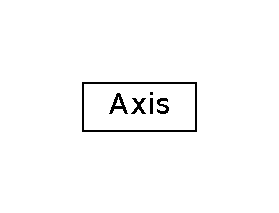
\includegraphics{inheritance-ecdec26b4dd4dc2ffb13ee9d91595cd439ae67e7.pdf}
\phantomsection\label{api/climlab.domain:module-climlab.domain.axis}\index{climlab.domain.axis (module)}\index{Axis (class in climlab.domain.axis)}

\begin{fulllineitems}
\phantomsection\label{api/climlab.domain:climlab.domain.axis.Axis}\pysiglinewithargsret{\strong{class }\code{climlab.domain.axis.}\bfcode{Axis}}{\emph{axis\_type='abstract'}, \emph{num\_points=10}, \emph{points=None}, \emph{bounds=None}}{}
Bases: \href{http://docs.python.org/2.7/library/functions.html\#object}{\code{object}}

Creates a new climlab Axis object.

An {\hyperref[api/climlab.domain:climlab.domain.axis.Axis]{\emph{\code{Axis}}}} (\autopageref*{api/climlab.domain:climlab.domain.axis.Axis}) is an object where information of a
spacial dimension of a {\hyperref[api/climlab.domain:climlab.domain.domain._Domain]{\emph{\code{\_Domain}}}} (\autopageref*{api/climlab.domain:climlab.domain.domain._Domain}) are specified.

These include the \emph{type} of the axis, the \emph{number of points}, location of 
\emph{points} and \emph{bounds} on the spatial dimension, magnitude of bounds
differences \emph{delta} as well as their \emph{unit}.

The \emph{axes} of a {\hyperref[api/climlab.domain:climlab.domain.domain._Domain]{\emph{\code{\_Domain}}}} (\autopageref*{api/climlab.domain:climlab.domain.domain._Domain}) are stored in the
dictionary axes, so they can be accessed through \code{dom.axes} if \code{dom} 
is an instance of {\hyperref[api/climlab.domain:climlab.domain.domain._Domain]{\emph{\code{\_Domain}}}} (\autopageref*{api/climlab.domain:climlab.domain.domain._Domain}).

\textbf{Initialization parameters}

An instance of \code{Axis} is initialized with the following 
arguments \emph{(for detailed information see Object attributes below)}:
\begin{quote}\begin{description}
\item[{Parameters}] \leavevmode\begin{itemize}
\item {} 
\textbf{\texttt{axis\_type}} (\href{http://docs.python.org/2.7/library/functions.html\#str}{\emph{\texttt{str}}}) -- information about the type of axis 
{[}default: `abstract'{]}

\item {} 
\textbf{\texttt{num\_points}} (\href{http://docs.python.org/2.7/library/functions.html\#int}{\emph{\texttt{int}}}) -- number of points on axis
{[}default: 10{]}

\item {} 
\textbf{\texttt{points}} (\href{http://docs.python.org/2.7/library/array.html\#module-array}{\emph{\texttt{array}}}) -- array with specific points (optional)

\item {} 
\textbf{\texttt{bounds}} (\href{http://docs.python.org/2.7/library/array.html\#module-array}{\emph{\texttt{array}}}) -- array with specific bounds between points (optional)

\end{itemize}

\item[{Raises}] \leavevmode
\code{ValueError}
if \code{axis\_type} is not one of the valid types or 
their euqivalents (see below).

\item[{Raises}] \leavevmode
\code{ValueError}
if \code{points} are given and not array-like.

\item[{Raises}] \leavevmode
\code{ValueError}
if \code{bounds} are given and not array-like.

\end{description}\end{quote}

\textbf{Object attributes}

Following object attributes are generated during initialization:
\begin{quote}\begin{description}
\item[{Variables}] \leavevmode\begin{itemize}
\item {} 
\textbf{\texttt{axis\_type}} (\href{http://docs.python.org/2.7/library/functions.html\#str}{\emph{\texttt{str}}}) -- 
Information about the type of axis. Valid axis types are:
\begin{itemize}
\item {} 
\code{'lev'}

\item {} 
\code{'lat'}

\item {} 
\code{'lon'}

\item {} 
\code{'depth'}

\item {} 
\code{'abstract'} (default)

\end{itemize}


\item {} 
\textbf{\texttt{num\_points}} (\href{http://docs.python.org/2.7/library/functions.html\#int}{\emph{\texttt{int}}}) -- number of points on axis

\item {} 
\textbf{\texttt{units}} (\href{http://docs.python.org/2.7/library/functions.html\#str}{\emph{\texttt{str}}}) -- Unit of the axis. During intialization the unit is 
chosen from the \code{defaultUnits} dictionary (see below).

\item {} 
\textbf{\texttt{points}} (\href{http://docs.python.org/2.7/library/array.html\#module-array}{\emph{\texttt{array}}}) -- array with all points of the axis (grid)

\item {} 
\textbf{\texttt{bounds}} (\href{http://docs.python.org/2.7/library/array.html\#module-array}{\emph{\texttt{array}}}) -- array with all bounds between points (staggered grid)

\item {} 
\textbf{\texttt{delta}} (\href{http://docs.python.org/2.7/library/array.html\#module-array}{\emph{\texttt{array}}}) -- array with spatial differences between bounds

\end{itemize}

\end{description}\end{quote}

\textbf{Axis Types}

A couple of differing axis type strings are rendered to valid axis types.
Alternate forms are listed here:
\begin{itemize}
\item {} \begin{description}
\item[{\code{'lev'}}] \leavevmode\begin{itemize}
\item {} 
\code{'p'}

\item {} 
\code{'press'}

\item {} 
\code{'pressure'}

\item {} 
\code{'P'}

\item {} 
\code{'Pressure'}

\item {} 
\code{'Press'}

\end{itemize}

\end{description}

\item {} \begin{description}
\item[{\code{'lat'}}] \leavevmode\begin{itemize}
\item {} 
\code{'Latitude'}

\item {} 
\code{'latitude'}

\end{itemize}

\end{description}

\item {} \begin{description}
\item[{\code{'lon'}}] \leavevmode\begin{itemize}
\item {} 
\code{'Longitude'}

\item {} 
\code{'longitude'}

\end{itemize}

\end{description}

\item {} \begin{description}
\item[{\code{'depth'}}] \leavevmode\begin{itemize}
\item {} 
\code{'Depth'}

\item {} 
\code{'waterDepth'}

\item {} 
\code{'water\_depth'}

\item {} 
\code{'slab'}

\end{itemize}

\end{description}

\end{itemize}

The \textbf{default units} are:

\begin{Verbatim}[commandchars=\\\{\}]
\PYG{n}{defaultUnits} \PYG{o}{=} \PYG{p}{\PYGZob{}}\PYG{l+s+s1}{\PYGZsq{}}\PYG{l+s+s1}{lev}\PYG{l+s+s1}{\PYGZsq{}}\PYG{p}{:} \PYG{l+s+s1}{\PYGZsq{}}\PYG{l+s+s1}{mb}\PYG{l+s+s1}{\PYGZsq{}}\PYG{p}{,}
                \PYG{l+s+s1}{\PYGZsq{}}\PYG{l+s+s1}{lat}\PYG{l+s+s1}{\PYGZsq{}}\PYG{p}{:} \PYG{l+s+s1}{\PYGZsq{}}\PYG{l+s+s1}{degrees}\PYG{l+s+s1}{\PYGZsq{}}\PYG{p}{,}
                \PYG{l+s+s1}{\PYGZsq{}}\PYG{l+s+s1}{lon}\PYG{l+s+s1}{\PYGZsq{}}\PYG{p}{:} \PYG{l+s+s1}{\PYGZsq{}}\PYG{l+s+s1}{degrees}\PYG{l+s+s1}{\PYGZsq{}}\PYG{p}{,}
                \PYG{l+s+s1}{\PYGZsq{}}\PYG{l+s+s1}{depth}\PYG{l+s+s1}{\PYGZsq{}}\PYG{p}{:} \PYG{l+s+s1}{\PYGZsq{}}\PYG{l+s+s1}{meters}\PYG{l+s+s1}{\PYGZsq{}}\PYG{p}{,}
                \PYG{l+s+s1}{\PYGZsq{}}\PYG{l+s+s1}{abstract}\PYG{l+s+s1}{\PYGZsq{}}\PYG{p}{:} \PYG{l+s+s1}{\PYGZsq{}}\PYG{l+s+s1}{none}\PYG{l+s+s1}{\PYGZsq{}}\PYG{p}{\PYGZcb{}}
\end{Verbatim}

If bounds are not given during initialization, \textbf{default end points} 
are used:

\begin{Verbatim}[commandchars=\\\{\}]
\PYG{n}{defaultEndPoints} \PYG{o}{=} \PYG{p}{\PYGZob{}}\PYG{l+s+s1}{\PYGZsq{}}\PYG{l+s+s1}{lev}\PYG{l+s+s1}{\PYGZsq{}}\PYG{p}{:} \PYG{p}{(}\PYG{l+m+mf}{0.}\PYG{p}{,} \PYG{n}{climlab}\PYG{o}{.}\PYG{n}{constants}\PYG{o}{.}\PYG{n}{ps}\PYG{p}{)}\PYG{p}{,}
                    \PYG{l+s+s1}{\PYGZsq{}}\PYG{l+s+s1}{lat}\PYG{l+s+s1}{\PYGZsq{}}\PYG{p}{:} \PYG{p}{(}\PYG{o}{\PYGZhy{}}\PYG{l+m+mf}{90.}\PYG{p}{,} \PYG{l+m+mf}{90.}\PYG{p}{)}\PYG{p}{,}
                    \PYG{l+s+s1}{\PYGZsq{}}\PYG{l+s+s1}{lon}\PYG{l+s+s1}{\PYGZsq{}}\PYG{p}{:} \PYG{p}{(}\PYG{l+m+mf}{0.}\PYG{p}{,} \PYG{l+m+mf}{360.}\PYG{p}{)}\PYG{p}{,}
                    \PYG{l+s+s1}{\PYGZsq{}}\PYG{l+s+s1}{depth}\PYG{l+s+s1}{\PYGZsq{}}\PYG{p}{:} \PYG{p}{(}\PYG{l+m+mf}{0.}\PYG{p}{,} \PYG{l+m+mf}{10.}\PYG{p}{)}\PYG{p}{,}
                    \PYG{l+s+s1}{\PYGZsq{}}\PYG{l+s+s1}{abstract}\PYG{l+s+s1}{\PYGZsq{}}\PYG{p}{:} \PYG{p}{(}\PYG{l+m+mi}{0}\PYG{p}{,} \PYG{n}{num\PYGZus{}points}\PYG{p}{)}\PYG{p}{\PYGZcb{}}
\end{Verbatim}
\begin{quote}\begin{description}
\item[{Example}] \leavevmode
Creation of a standalone Axis:

\begin{Verbatim}[commandchars=\\\{\}]
\PYG{g+gp}{\PYGZgt{}\PYGZgt{}\PYGZgt{} }\PYG{k+kn}{import} \PYG{n+nn}{climlab}
\PYG{g+gp}{\PYGZgt{}\PYGZgt{}\PYGZgt{} }\PYG{n}{ax} \PYG{o}{=} \PYG{n}{climlab}\PYG{o}{.}\PYG{n}{domain}\PYG{o}{.}\PYG{n}{Axis}\PYG{p}{(}\PYG{n}{axis\PYGZus{}type}\PYG{o}{=}\PYG{l+s+s1}{\PYGZsq{}}\PYG{l+s+s1}{Latitude}\PYG{l+s+s1}{\PYGZsq{}}\PYG{p}{,} \PYG{n}{num\PYGZus{}points}\PYG{o}{=}\PYG{l+m+mi}{36}\PYG{p}{)}

\PYG{g+gp}{\PYGZgt{}\PYGZgt{}\PYGZgt{} }\PYG{k}{print} \PYG{n}{ax}
\PYG{g+go}{Axis of type lat with 36 points.}

\PYG{g+gp}{\PYGZgt{}\PYGZgt{}\PYGZgt{} }\PYG{n}{ax}\PYG{o}{.}\PYG{n}{points}
\PYG{g+go}{array([\PYGZhy{}87.5, \PYGZhy{}82.5, \PYGZhy{}77.5, \PYGZhy{}72.5, \PYGZhy{}67.5, \PYGZhy{}62.5, \PYGZhy{}57.5, \PYGZhy{}52.5, \PYGZhy{}47.5,}
\PYG{g+go}{       \PYGZhy{}42.5, \PYGZhy{}37.5, \PYGZhy{}32.5, \PYGZhy{}27.5, \PYGZhy{}22.5, \PYGZhy{}17.5, \PYGZhy{}12.5,  \PYGZhy{}7.5,  \PYGZhy{}2.5,}
\PYG{g+go}{         2.5,   7.5,  12.5,  17.5,  22.5,  27.5,  32.5,  37.5,  42.5,}
\PYG{g+go}{        47.5,  52.5,  57.5,  62.5,  67.5,  72.5,  77.5,  82.5,  87.5])}

\PYG{g+gp}{\PYGZgt{}\PYGZgt{}\PYGZgt{} }\PYG{n}{ax}\PYG{o}{.}\PYG{n}{bounds}
\PYG{g+go}{array([\PYGZhy{}90., \PYGZhy{}85., \PYGZhy{}80., \PYGZhy{}75., \PYGZhy{}70., \PYGZhy{}65., \PYGZhy{}60., \PYGZhy{}55., \PYGZhy{}50., \PYGZhy{}45., \PYGZhy{}40.,}
\PYG{g+go}{       \PYGZhy{}35., \PYGZhy{}30., \PYGZhy{}25., \PYGZhy{}20., \PYGZhy{}15., \PYGZhy{}10.,  \PYGZhy{}5.,   0.,   5.,  10.,  15.,}
\PYG{g+go}{        20.,  25.,  30.,  35.,  40.,  45.,  50.,  55.,  60.,  65.,  70.,}
\PYG{g+go}{        75.,  80.,  85.,  90.])}

\PYG{g+gp}{\PYGZgt{}\PYGZgt{}\PYGZgt{} }\PYG{n}{ax}\PYG{o}{.}\PYG{n}{delta}
\PYG{g+go}{array([ 5.,  5.,  5.,  5.,  5.,  5.,  5.,  5.,  5.,  5.,  5.,  5.,  5.,}
\PYG{g+go}{        5.,  5.,  5.,  5.,  5.,  5.,  5.,  5.,  5.,  5.,  5.,  5.,  5.,}
\PYG{g+go}{        5.,  5.,  5.,  5.,  5.,  5.,  5.,  5.,  5.,  5.])   }
\end{Verbatim}

\end{description}\end{quote}

\end{fulllineitems}



\subsubsection{climlab.domain.domain module}
\label{api/climlab.domain:climlab-domain-domain-module}
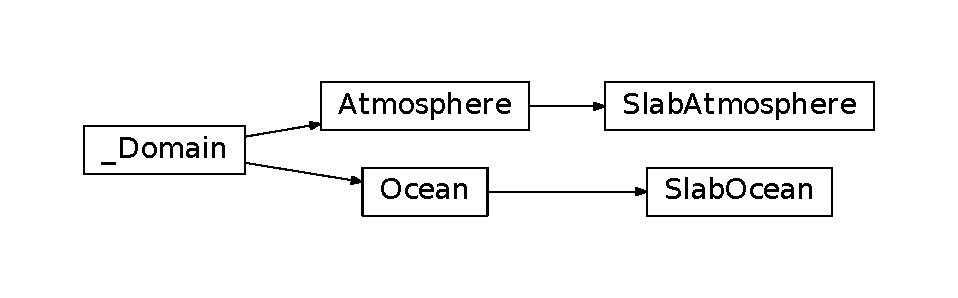
\includegraphics{inheritance-370eb7bb9929bc3993457a6ca9fc0b68128e90d7.pdf}
\phantomsection\label{api/climlab.domain:module-climlab.domain.domain}\index{climlab.domain.domain (module)}\index{Atmosphere (class in climlab.domain.domain)}

\begin{fulllineitems}
\phantomsection\label{api/climlab.domain:climlab.domain.domain.Atmosphere}\pysiglinewithargsret{\strong{class }\code{climlab.domain.domain.}\bfcode{Atmosphere}}{\emph{**kwargs}}{}
Bases: {\hyperref[api/climlab.domain:climlab.domain.domain._Domain]{\emph{\code{climlab.domain.domain.\_Domain}}}} (\autopageref*{api/climlab.domain:climlab.domain.domain._Domain})

Class for the implementation of an Atmosphere Domain.

\textbf{Object attributes}

Additional to the parent class {\hyperref[api/climlab.domain:climlab.domain.domain._Domain]{\emph{\code{\_Domain}}}} (\autopageref*{api/climlab.domain:climlab.domain.domain._Domain})
the following object attribute is modified during initialization:
\begin{quote}\begin{description}
\item[{Variables}] \leavevmode
\textbf{\texttt{domain\_type}} (\href{http://docs.python.org/2.7/library/functions.html\#str}{\emph{\texttt{str}}}) -- is set to \code{'atm'}

\item[{Example}] \leavevmode
Setting up an Atmosphere Domain:

\begin{Verbatim}[commandchars=\\\{\}]
\PYG{g+gp}{\PYGZgt{}\PYGZgt{}\PYGZgt{} }\PYG{k+kn}{import} \PYG{n+nn}{climlab}
\PYG{g+gp}{\PYGZgt{}\PYGZgt{}\PYGZgt{} }\PYG{n}{atm\PYGZus{}ax} \PYG{o}{=} \PYG{n}{climlab}\PYG{o}{.}\PYG{n}{domain}\PYG{o}{.}\PYG{n}{Axis}\PYG{p}{(}\PYG{n}{axis\PYGZus{}type}\PYG{o}{=}\PYG{l+s+s1}{\PYGZsq{}}\PYG{l+s+s1}{pressure}\PYG{l+s+s1}{\PYGZsq{}}\PYG{p}{,} \PYG{n}{num\PYGZus{}points}\PYG{o}{=}\PYG{l+m+mi}{10}\PYG{p}{)}
\PYG{g+gp}{\PYGZgt{}\PYGZgt{}\PYGZgt{} }\PYG{n}{atm\PYGZus{}domain} \PYG{o}{=} \PYG{n}{climlab}\PYG{o}{.}\PYG{n}{domain}\PYG{o}{.}\PYG{n}{Atmosphere}\PYG{p}{(}\PYG{n}{axes}\PYG{o}{=}\PYG{n}{atm\PYGZus{}ax}\PYG{p}{)}

\PYG{g+gp}{\PYGZgt{}\PYGZgt{}\PYGZgt{} }\PYG{k}{print} \PYG{n}{atm\PYGZus{}domain}
\PYG{g+go}{climlab Domain object with domain\PYGZus{}type=atm and shape=(10,)}

\PYG{g+gp}{\PYGZgt{}\PYGZgt{}\PYGZgt{} }\PYG{n}{atm\PYGZus{}domain}\PYG{o}{.}\PYG{n}{axes}
\PYG{g+go}{\PYGZob{}\PYGZsq{}lev\PYGZsq{}: \PYGZlt{}climlab.domain.axis.Axis object at 0x7fe5b8ef8e10\PYGZgt{}\PYGZcb{}}

\PYG{g+gp}{\PYGZgt{}\PYGZgt{}\PYGZgt{} }\PYG{n}{atm\PYGZus{}domain}\PYG{o}{.}\PYG{n}{heat\PYGZus{}capacity}
\PYG{g+go}{array([ 1024489.79591837,  1024489.79591837,  1024489.79591837,}
\PYG{g+go}{        1024489.79591837,  1024489.79591837,  1024489.79591837,}
\PYG{g+go}{        1024489.79591837,  1024489.79591837,  1024489.79591837,}
\PYG{g+go}{        1024489.79591837])}
\end{Verbatim}

\end{description}\end{quote}
\index{set\_heat\_capacity() (climlab.domain.domain.Atmosphere method)}

\begin{fulllineitems}
\phantomsection\label{api/climlab.domain:climlab.domain.domain.Atmosphere.set_heat_capacity}\pysiglinewithargsret{\bfcode{set\_heat\_capacity}}{}{}
Sets the heat capacity of the Atmosphere Domain.

Calls the utils heat capacity function 
{\hyperref[api/climlab.utils:climlab.utils.heat_capacity.atmosphere]{\emph{\code{atmosphere()}}}} (\autopageref*{api/climlab.utils:climlab.utils.heat_capacity.atmosphere}) and gives the delta 
array of grid points of it's level axis
\code{self.axes{[}'lev'{]}.delta} as input.

\textbf{Object attributes}

During method execution following object attribute is modified:
\begin{quote}\begin{description}
\item[{Variables}] \leavevmode
{\hyperref[api/climlab.utils:module\string-climlab.utils.heat_capacity]{\emph{\textbf{\texttt{heat\_capacity}}}}} (\autopageref*{api/climlab.utils:module-climlab.utils.heat_capacity}) (\href{http://docs.python.org/2.7/library/array.html\#module-array}{\emph{\texttt{array}}}) -- the ocean domain's heat capacity over 
the \code{'lev'} Axis.

\end{description}\end{quote}

\end{fulllineitems}


\end{fulllineitems}

\index{Ocean (class in climlab.domain.domain)}

\begin{fulllineitems}
\phantomsection\label{api/climlab.domain:climlab.domain.domain.Ocean}\pysiglinewithargsret{\strong{class }\code{climlab.domain.domain.}\bfcode{Ocean}}{\emph{**kwargs}}{}
Bases: {\hyperref[api/climlab.domain:climlab.domain.domain._Domain]{\emph{\code{climlab.domain.domain.\_Domain}}}} (\autopageref*{api/climlab.domain:climlab.domain.domain._Domain})

Class for the implementation of an Ocean Domain.

\textbf{Object attributes}

Additional to the parent class {\hyperref[api/climlab.domain:climlab.domain.domain._Domain]{\emph{\code{\_Domain}}}} (\autopageref*{api/climlab.domain:climlab.domain.domain._Domain})
the following object attribute is modified during initialization:
\begin{quote}\begin{description}
\item[{Variables}] \leavevmode
\textbf{\texttt{domain\_type}} (\href{http://docs.python.org/2.7/library/functions.html\#str}{\emph{\texttt{str}}}) -- is set to \code{'ocean'}

\item[{Example}] \leavevmode
Setting up an Ocean Domain:

\begin{Verbatim}[commandchars=\\\{\}]
\PYG{g+gp}{\PYGZgt{}\PYGZgt{}\PYGZgt{} }\PYG{k+kn}{import} \PYG{n+nn}{climlab}
\PYG{g+gp}{\PYGZgt{}\PYGZgt{}\PYGZgt{} }\PYG{n}{ocean\PYGZus{}ax} \PYG{o}{=} \PYG{n}{climlab}\PYG{o}{.}\PYG{n}{domain}\PYG{o}{.}\PYG{n}{Axis}\PYG{p}{(}\PYG{n}{axis\PYGZus{}type}\PYG{o}{=}\PYG{l+s+s1}{\PYGZsq{}}\PYG{l+s+s1}{depth}\PYG{l+s+s1}{\PYGZsq{}}\PYG{p}{,} \PYG{n}{num\PYGZus{}points}\PYG{o}{=}\PYG{l+m+mi}{5}\PYG{p}{)}
\PYG{g+gp}{\PYGZgt{}\PYGZgt{}\PYGZgt{} }\PYG{n}{ocean\PYGZus{}domain} \PYG{o}{=} \PYG{n}{climlab}\PYG{o}{.}\PYG{n}{domain}\PYG{o}{.}\PYG{n}{Ocean}\PYG{p}{(}\PYG{n}{axes}\PYG{o}{=}\PYG{n}{ocean\PYGZus{}ax}\PYG{p}{)}

\PYG{g+gp}{\PYGZgt{}\PYGZgt{}\PYGZgt{} }\PYG{k}{print} \PYG{n}{ocean\PYGZus{}domain}
\PYG{g+go}{climlab Domain object with domain\PYGZus{}type=ocean and shape=(5,)}

\PYG{g+gp}{\PYGZgt{}\PYGZgt{}\PYGZgt{} }\PYG{n}{ocean\PYGZus{}domain}\PYG{o}{.}\PYG{n}{axes}
\PYG{g+go}{\PYGZob{}\PYGZsq{}depth\PYGZsq{}: \PYGZlt{}climlab.domain.axis.Axis object at 0x7fe5b8f102d0\PYGZgt{}\PYGZcb{}}

\PYG{g+gp}{\PYGZgt{}\PYGZgt{}\PYGZgt{} }\PYG{n}{ocean\PYGZus{}domain}\PYG{o}{.}\PYG{n}{heat\PYGZus{}capacity}
\PYG{g+go}{array([ 8362600.,  8362600.,  8362600.,  8362600.,  8362600.])}
\end{Verbatim}

\end{description}\end{quote}
\index{set\_heat\_capacity() (climlab.domain.domain.Ocean method)}

\begin{fulllineitems}
\phantomsection\label{api/climlab.domain:climlab.domain.domain.Ocean.set_heat_capacity}\pysiglinewithargsret{\bfcode{set\_heat\_capacity}}{}{}
Sets the heat capacity of the Ocean Domain.

Calls the utils heat capacity function 
{\hyperref[api/climlab.utils:climlab.utils.heat_capacity.ocean]{\emph{\code{ocean()}}}} (\autopageref*{api/climlab.utils:climlab.utils.heat_capacity.ocean}) and gives the delta 
array of grid points of it's depth axis
\code{self.axes{[}'depth'{]}.delta} as input.

\textbf{Object attributes}

During method execution following object attribute is modified:
\begin{quote}\begin{description}
\item[{Variables}] \leavevmode
{\hyperref[api/climlab.utils:module\string-climlab.utils.heat_capacity]{\emph{\textbf{\texttt{heat\_capacity}}}}} (\autopageref*{api/climlab.utils:module-climlab.utils.heat_capacity}) (\href{http://docs.python.org/2.7/library/array.html\#module-array}{\emph{\texttt{array}}}) -- the ocean domain's heat capacity over 
the \code{'depth'} Axis.

\end{description}\end{quote}

\end{fulllineitems}


\end{fulllineitems}

\index{SlabAtmosphere (class in climlab.domain.domain)}

\begin{fulllineitems}
\phantomsection\label{api/climlab.domain:climlab.domain.domain.SlabAtmosphere}\pysiglinewithargsret{\strong{class }\code{climlab.domain.domain.}\bfcode{SlabAtmosphere}}{\emph{axes=\textless{}climlab.domain.axis.Axis object\textgreater{}}, \emph{**kwargs}}{}
Bases: {\hyperref[api/climlab.domain:climlab.domain.domain.Atmosphere]{\emph{\code{climlab.domain.domain.Atmosphere}}}} (\autopageref*{api/climlab.domain:climlab.domain.domain.Atmosphere})

A class to create a SlabAtmosphere Domain by default.

Initializes the parent {\hyperref[api/climlab.domain:climlab.domain.domain.Atmosphere]{\emph{\code{Atmosphere}}}} (\autopageref*{api/climlab.domain:climlab.domain.domain.Atmosphere}) class with a simple axis for a
Slab Atmopshere created by {\hyperref[api/climlab.domain:climlab.domain.domain.make_slabatm_axis]{\emph{\code{make\_slabatm\_axis()}}}} (\autopageref*{api/climlab.domain:climlab.domain.domain.make_slabatm_axis}) which has just 1 cell 
in height by default.
\begin{quote}\begin{description}
\item[{Example}] \leavevmode
Creating a SlabAtmosphere Domain:

\begin{Verbatim}[commandchars=\\\{\}]
\PYG{g+gp}{\PYGZgt{}\PYGZgt{}\PYGZgt{} }\PYG{k+kn}{import} \PYG{n+nn}{climlab}
\PYG{g+gp}{\PYGZgt{}\PYGZgt{}\PYGZgt{} }\PYG{n}{slab\PYGZus{}atm\PYGZus{}domain} \PYG{o}{=} \PYG{n}{climlab}\PYG{o}{.}\PYG{n}{domain}\PYG{o}{.}\PYG{n}{SlabAtmosphere}\PYG{p}{(}\PYG{p}{)}

\PYG{g+gp}{\PYGZgt{}\PYGZgt{}\PYGZgt{} }\PYG{k}{print} \PYG{n}{slab\PYGZus{}atm\PYGZus{}domain}
\PYG{g+go}{climlab Domain object with domain\PYGZus{}type=atm and shape=(1,)}

\PYG{g+gp}{\PYGZgt{}\PYGZgt{}\PYGZgt{} }\PYG{n}{slab\PYGZus{}atm\PYGZus{}domain}\PYG{o}{.}\PYG{n}{axes}
\PYG{g+go}{\PYGZob{}\PYGZsq{}lev\PYGZsq{}: \PYGZlt{}climlab.domain.axis.Axis object at 0x7fe5c4281610\PYGZgt{}\PYGZcb{}}

\PYG{g+gp}{\PYGZgt{}\PYGZgt{}\PYGZgt{} }\PYG{n}{slab\PYGZus{}atm\PYGZus{}domain}\PYG{o}{.}\PYG{n}{heat\PYGZus{}capacity}
\PYG{g+go}{array([ 10244897.95918367])}
\end{Verbatim}

\end{description}\end{quote}

\end{fulllineitems}

\index{SlabOcean (class in climlab.domain.domain)}

\begin{fulllineitems}
\phantomsection\label{api/climlab.domain:climlab.domain.domain.SlabOcean}\pysiglinewithargsret{\strong{class }\code{climlab.domain.domain.}\bfcode{SlabOcean}}{\emph{axes=\textless{}climlab.domain.axis.Axis object\textgreater{}}, \emph{**kwargs}}{}
Bases: {\hyperref[api/climlab.domain:climlab.domain.domain.Ocean]{\emph{\code{climlab.domain.domain.Ocean}}}} (\autopageref*{api/climlab.domain:climlab.domain.domain.Ocean})

A class to create a SlabOcean Domain by default.

Initializes the parent {\hyperref[api/climlab.domain:climlab.domain.domain.Ocean]{\emph{\code{Ocean}}}} (\autopageref*{api/climlab.domain:climlab.domain.domain.Ocean}) class with a simple axis for a
Slab Ocean created by {\hyperref[api/climlab.domain:climlab.domain.domain.make_slabocean_axis]{\emph{\code{make\_slabocean\_axis()}}}} (\autopageref*{api/climlab.domain:climlab.domain.domain.make_slabocean_axis}) which has just 1 cell 
in depth by default.
\begin{quote}\begin{description}
\item[{Example}] \leavevmode
Creating a SlabOcean Domain:

\begin{Verbatim}[commandchars=\\\{\}]
\PYG{g+gp}{\PYGZgt{}\PYGZgt{}\PYGZgt{} }\PYG{k+kn}{import} \PYG{n+nn}{climlab}
\PYG{g+gp}{\PYGZgt{}\PYGZgt{}\PYGZgt{} }\PYG{n}{slab\PYGZus{}ocean\PYGZus{}domain} \PYG{o}{=} \PYG{n}{climlab}\PYG{o}{.}\PYG{n}{domain}\PYG{o}{.}\PYG{n}{SlabOcean}\PYG{p}{(}\PYG{p}{)}

\PYG{g+gp}{\PYGZgt{}\PYGZgt{}\PYGZgt{} }\PYG{k}{print} \PYG{n}{slab\PYGZus{}ocean\PYGZus{}domain}
\PYG{g+go}{climlab Domain object with domain\PYGZus{}type=ocean and shape=(1,)}

\PYG{g+gp}{\PYGZgt{}\PYGZgt{}\PYGZgt{} }\PYG{n}{slab\PYGZus{}ocean\PYGZus{}domain}\PYG{o}{.}\PYG{n}{axes}
\PYG{g+go}{\PYGZob{}\PYGZsq{}depth\PYGZsq{}: \PYGZlt{}climlab.domain.axis.Axis object at 0x7fe5c42814d0\PYGZgt{}\PYGZcb{}}

\PYG{g+gp}{\PYGZgt{}\PYGZgt{}\PYGZgt{} }\PYG{n}{slab\PYGZus{}ocean\PYGZus{}domain}\PYG{o}{.}\PYG{n}{heat\PYGZus{}capacity}
\PYG{g+go}{array([ 41813000.])    }
\end{Verbatim}

\end{description}\end{quote}

\end{fulllineitems}

\index{\_Domain (class in climlab.domain.domain)}

\begin{fulllineitems}
\phantomsection\label{api/climlab.domain:climlab.domain.domain._Domain}\pysiglinewithargsret{\strong{class }\code{climlab.domain.domain.}\bfcode{\_Domain}}{\emph{axes=None}, \emph{**kwargs}}{}
Bases: \href{http://docs.python.org/2.7/library/functions.html\#object}{\code{object}}

Private parent class for \emph{Domains}.

A \emph{Domain} defines an area or spatial base for a climlab 
{\hyperref[api/climlab.process:climlab.process.process.Process]{\emph{\code{Process}}}} (\autopageref*{api/climlab.process:climlab.process.process.Process}) object. It consists of axes which
are {\hyperref[api/climlab.domain:climlab.domain.axis.Axis]{\emph{\code{Axis}}}} (\autopageref*{api/climlab.domain:climlab.domain.axis.Axis}) objects that define the dimensions 
of the \emph{Domain}.

In a \emph{Domain} the heat capacity of grid points, bounds or cells/boxes is 
specified.

There are daughter classes {\hyperref[api/climlab.domain:climlab.domain.domain.Atmosphere]{\emph{\code{Atmosphere}}}} (\autopageref*{api/climlab.domain:climlab.domain.domain.Atmosphere}) and
{\hyperref[api/climlab.domain:climlab.domain.domain.Ocean]{\emph{\code{Ocean}}}} (\autopageref*{api/climlab.domain:climlab.domain.domain.Ocean}) of the private 
{\hyperref[api/climlab.domain:climlab.domain.domain._Domain]{\emph{\code{\_Domain}}}} (\autopageref*{api/climlab.domain:climlab.domain.domain._Domain}) class implemented which themselves 
have daughter classes {\hyperref[api/climlab.domain:climlab.domain.domain.SlabAtmosphere]{\emph{\code{SlabAtmosphere}}}} (\autopageref*{api/climlab.domain:climlab.domain.domain.SlabAtmosphere}) and 
{\hyperref[api/climlab.domain:climlab.domain.domain.SlabOcean]{\emph{\code{SlabOcean}}}} (\autopageref*{api/climlab.domain:climlab.domain.domain.SlabOcean}).

Several methods are implemented that create \emph{Domains} with special 
specifications. These are
\begin{itemize}
\item {} 
{\hyperref[api/climlab.domain:climlab.domain.domain.single_column]{\emph{\code{single\_column()}}}} (\autopageref*{api/climlab.domain:climlab.domain.domain.single_column})

\item {} 
{\hyperref[api/climlab.domain:climlab.domain.domain.zonal_mean_column]{\emph{\code{zonal\_mean\_column()}}}} (\autopageref*{api/climlab.domain:climlab.domain.domain.zonal_mean_column})

\item {} 
{\hyperref[api/climlab.domain:climlab.domain.domain.box_model_domain]{\emph{\code{box\_model\_domain()}}}} (\autopageref*{api/climlab.domain:climlab.domain.domain.box_model_domain})

\end{itemize}

\textbf{Initialization parameters}

An instance of \code{\_Domain} is initialized with the following 
arguments:
\begin{quote}\begin{description}
\item[{Parameters}] \leavevmode
\textbf{\texttt{axes}} (dict or {\hyperref[api/climlab.domain:climlab.domain.axis.Axis]{\emph{\code{Axis}}}} (\autopageref*{api/climlab.domain:climlab.domain.axis.Axis})) -- Axis object or dictionary of Axis object where domain will
be defined on.

\end{description}\end{quote}

\textbf{Object attributes}

Following object attributes are generated during initialization:
\begin{quote}\begin{description}
\item[{Variables}] \leavevmode\begin{itemize}
\item {} 
\textbf{\texttt{domain\_type}} (\href{http://docs.python.org/2.7/library/functions.html\#str}{\emph{\texttt{str}}}) -- Set to \code{'undefined'}.

\item {} 
\textbf{\texttt{axes}} (\href{http://docs.python.org/2.7/library/stdtypes.html\#dict}{\emph{\texttt{dict}}}) -- A dictionary of the domains axes. Created by
{\hyperref[api/climlab.domain:climlab.domain.domain._Domain._make_axes_dict]{\emph{\code{\_make\_axes\_dict()}}}} (\autopageref*{api/climlab.domain:climlab.domain.domain._Domain._make_axes_dict}) called with input 
argument \code{axes}

\item {} 
\textbf{\texttt{numdims}} (\href{http://docs.python.org/2.7/library/functions.html\#int}{\emph{\texttt{int}}}) -- Number of {\hyperref[api/climlab.domain:climlab.domain.axis.Axis]{\emph{\code{Axis}}}} (\autopageref*{api/climlab.domain:climlab.domain.axis.Axis}) objects
in \code{self.axes} dictionary.

\item {} 
\textbf{\texttt{ax\_index}} (\href{http://docs.python.org/2.7/library/stdtypes.html\#dict}{\emph{\texttt{dict}}}) -- 
A dictionary of domain axes and their corresponding index
in an ordered list of the axes with:
\begin{itemize}
\item {} 
\code{'lev'} or \code{'depth'} is last

\item {} 
\code{'lat'} is second last

\end{itemize}


\item {} 
\textbf{\texttt{shape}} (\href{http://docs.python.org/2.7/library/functions.html\#tuple}{\emph{\texttt{tuple}}}) -- Number of points of all domain axes. Order in 
tuple given by \code{self.ax\_index}.

\item {} 
{\hyperref[api/climlab.utils:module\string-climlab.utils.heat_capacity]{\emph{\textbf{\texttt{heat\_capacity}}}}} (\autopageref*{api/climlab.utils:module-climlab.utils.heat_capacity}) (\href{http://docs.python.org/2.7/library/array.html\#module-array}{\emph{\texttt{array}}}) -- the domain's heat capacity over axis specified 
in function call of {\hyperref[api/climlab.domain:climlab.domain.domain._Domain.set_heat_capacity]{\emph{\code{set\_heat\_capacity()}}}} (\autopageref*{api/climlab.domain:climlab.domain.domain._Domain.set_heat_capacity})

\end{itemize}

\end{description}\end{quote}
\index{\_make\_axes\_dict() (climlab.domain.domain.\_Domain method)}

\begin{fulllineitems}
\phantomsection\label{api/climlab.domain:climlab.domain.domain._Domain._make_axes_dict}\pysiglinewithargsret{\bfcode{\_make\_axes\_dict}}{\emph{axes}}{}
Makes an axes dictionary.

\begin{notice}{note}{Note:}
In case the input is \code{None}, the dictionary \code{\{'empty': None\}}
is returned.
\end{notice}

\textbf{Function-call argument}
\begin{quote}\begin{description}
\item[{Parameters}] \leavevmode
\textbf{\texttt{axes}} (dict or single instance of 
{\hyperref[api/climlab.domain:climlab.domain.axis.Axis]{\emph{\code{Axis}}}} (\autopageref*{api/climlab.domain:climlab.domain.axis.Axis}) object or \code{None}) -- axes input

\item[{Raises}] \leavevmode
\code{ValueError}  if input is not an instance of Axis class 
or a dictionary of Axis objetcs

\item[{Returns}] \leavevmode
dictionary of input axes

\item[{Return type}] \leavevmode
\href{http://docs.python.org/2.7/library/stdtypes.html\#dict}{dict}

\end{description}\end{quote}

\end{fulllineitems}

\index{set\_heat\_capacity() (climlab.domain.domain.\_Domain method)}

\begin{fulllineitems}
\phantomsection\label{api/climlab.domain:climlab.domain.domain._Domain.set_heat_capacity}\pysiglinewithargsret{\bfcode{set\_heat\_capacity}}{}{}
A dummy function to set the heat capacity of a domain.

\emph{Should be overridden by daugter classes.}

\end{fulllineitems}


\end{fulllineitems}

\index{box\_model\_domain() (in module climlab.domain.domain)}

\begin{fulllineitems}
\phantomsection\label{api/climlab.domain:climlab.domain.domain.box_model_domain}\pysiglinewithargsret{\code{climlab.domain.domain.}\bfcode{box\_model\_domain}}{\emph{num\_points=2}, \emph{**kwargs}}{}
Creates a box model domain (a single abstract axis).
\begin{quote}\begin{description}
\item[{Parameters}] \leavevmode
\textbf{\texttt{num\_points}} (\href{http://docs.python.org/2.7/library/functions.html\#int}{\emph{\texttt{int}}}) -- number of boxes {[}default: 2{]}

\item[{Returns}] \leavevmode
Domain with single axis of type \code{'abstract'} 
and \code{self.domain\_type = 'box'}

\item[{Return type}] \leavevmode
{\hyperref[api/climlab.domain:climlab.domain.domain._Domain]{\emph{\code{\_Domain}}}} (\autopageref*{api/climlab.domain:climlab.domain.domain._Domain})

\item[{Example}] \leavevmode
\begin{Verbatim}[commandchars=\\\{\}]
\PYG{g+gp}{\PYGZgt{}\PYGZgt{}\PYGZgt{} }\PYG{k+kn}{from} \PYG{n+nn}{climlab} \PYG{k+kn}{import} \PYG{n}{domain}
\PYG{g+gp}{\PYGZgt{}\PYGZgt{}\PYGZgt{} }\PYG{n}{box} \PYG{o}{=} \PYG{n}{domain}\PYG{o}{.}\PYG{n}{box\PYGZus{}model\PYGZus{}domain}\PYG{p}{(}\PYG{n}{num\PYGZus{}points}\PYG{o}{=}\PYG{l+m+mi}{2}\PYG{p}{)}

\PYG{g+gp}{\PYGZgt{}\PYGZgt{}\PYGZgt{} }\PYG{k}{print} \PYG{n}{box}
\PYG{g+go}{climlab Domain object with domain\PYGZus{}type=box and shape=(2,)    }
\end{Verbatim}

\end{description}\end{quote}

\end{fulllineitems}

\index{make\_slabatm\_axis() (in module climlab.domain.domain)}

\begin{fulllineitems}
\phantomsection\label{api/climlab.domain:climlab.domain.domain.make_slabatm_axis}\pysiglinewithargsret{\code{climlab.domain.domain.}\bfcode{make\_slabatm\_axis}}{\emph{num\_points=1}}{}
Convenience method to create a simple axis for a slab atmosphere.

\textbf{Function-call argument}
\begin{quote}\begin{description}
\item[{Parameters}] \leavevmode
\textbf{\texttt{num\_points}} (\href{http://docs.python.org/2.7/library/functions.html\#int}{\emph{\texttt{int}}}) -- number of points for the slabatmosphere Axis {[}default: 1{]}

\item[{Returns}] \leavevmode
an Axis with \code{axis\_type='lev'} and \code{num\_points=num\_points}

\item[{Return type}] \leavevmode
{\hyperref[api/climlab.domain:climlab.domain.axis.Axis]{\emph{\code{Axis}}}} (\autopageref*{api/climlab.domain:climlab.domain.axis.Axis})

\item[{Example}] \leavevmode
\begin{Verbatim}[commandchars=\\\{\}]
\PYG{g+gp}{\PYGZgt{}\PYGZgt{}\PYGZgt{} }\PYG{k+kn}{import} \PYG{n+nn}{climlab}
\PYG{g+gp}{\PYGZgt{}\PYGZgt{}\PYGZgt{} }\PYG{n}{slab\PYGZus{}atm\PYGZus{}axis} \PYG{o}{=} \PYG{n}{climlab}\PYG{o}{.}\PYG{n}{domain}\PYG{o}{.}\PYG{n}{make\PYGZus{}slabatm\PYGZus{}axis}\PYG{p}{(}\PYG{p}{)}

\PYG{g+gp}{\PYGZgt{}\PYGZgt{}\PYGZgt{} }\PYG{k}{print} \PYG{n}{slab\PYGZus{}atm\PYGZus{}axis}
\PYG{g+go}{Axis of type lev with 1 points.}

\PYG{g+gp}{\PYGZgt{}\PYGZgt{}\PYGZgt{} }\PYG{n}{slab\PYGZus{}atm\PYGZus{}axis}\PYG{o}{.}\PYG{n}{axis\PYGZus{}type}
\PYG{g+go}{\PYGZsq{}lev\PYGZsq{}}

\PYG{g+gp}{\PYGZgt{}\PYGZgt{}\PYGZgt{} }\PYG{n}{slab\PYGZus{}atm\PYGZus{}axis}\PYG{o}{.}\PYG{n}{bounds}
\PYG{g+go}{array([    0.,  1000.])}

\PYG{g+gp}{\PYGZgt{}\PYGZgt{}\PYGZgt{} }\PYG{n}{slab\PYGZus{}atm\PYGZus{}axis}\PYG{o}{.}\PYG{n}{units}
\PYG{g+go}{\PYGZsq{}mb\PYGZsq{}     }
\end{Verbatim}

\end{description}\end{quote}

\end{fulllineitems}

\index{make\_slabocean\_axis() (in module climlab.domain.domain)}

\begin{fulllineitems}
\phantomsection\label{api/climlab.domain:climlab.domain.domain.make_slabocean_axis}\pysiglinewithargsret{\code{climlab.domain.domain.}\bfcode{make\_slabocean\_axis}}{\emph{num\_points=1}}{}
Convenience method to create a simple axis for a slab ocean.

\textbf{Function-call argument}
\begin{quote}\begin{description}
\item[{Parameters}] \leavevmode
\textbf{\texttt{num\_points}} (\href{http://docs.python.org/2.7/library/functions.html\#int}{\emph{\texttt{int}}}) -- number of points for the slabocean Axis {[}default: 1{]}

\item[{Returns}] \leavevmode
an Axis with \code{axis\_type='depth'} and \code{num\_points=num\_points}

\item[{Return type}] \leavevmode
{\hyperref[api/climlab.domain:climlab.domain.axis.Axis]{\emph{\code{Axis}}}} (\autopageref*{api/climlab.domain:climlab.domain.axis.Axis})

\item[{Example}] \leavevmode
\begin{Verbatim}[commandchars=\\\{\}]
\PYG{g+gp}{\PYGZgt{}\PYGZgt{}\PYGZgt{} }\PYG{k+kn}{import} \PYG{n+nn}{climlab}
\PYG{g+gp}{\PYGZgt{}\PYGZgt{}\PYGZgt{} }\PYG{n}{slab\PYGZus{}ocean\PYGZus{}axis} \PYG{o}{=} \PYG{n}{climlab}\PYG{o}{.}\PYG{n}{domain}\PYG{o}{.}\PYG{n}{make\PYGZus{}slabocean\PYGZus{}axis}\PYG{p}{(}\PYG{p}{)}

\PYG{g+gp}{\PYGZgt{}\PYGZgt{}\PYGZgt{} }\PYG{k}{print} \PYG{n}{slab\PYGZus{}ocean\PYGZus{}axis}
\PYG{g+go}{Axis of type depth with 1 points.}

\PYG{g+gp}{\PYGZgt{}\PYGZgt{}\PYGZgt{} }\PYG{n}{slab\PYGZus{}ocean\PYGZus{}axis}\PYG{o}{.}\PYG{n}{axis\PYGZus{}type}
\PYG{g+go}{\PYGZsq{}depth\PYGZsq{}}

\PYG{g+gp}{\PYGZgt{}\PYGZgt{}\PYGZgt{} }\PYG{n}{slab\PYGZus{}ocean\PYGZus{}axis}\PYG{o}{.}\PYG{n}{bounds}
\PYG{g+go}{array([  0.,  10.])}

\PYG{g+gp}{\PYGZgt{}\PYGZgt{}\PYGZgt{} }\PYG{n}{slab\PYGZus{}ocean\PYGZus{}axis}\PYG{o}{.}\PYG{n}{units}
\PYG{g+go}{\PYGZsq{}meters\PYGZsq{}                 }
\end{Verbatim}

\end{description}\end{quote}

\end{fulllineitems}

\index{single\_column() (in module climlab.domain.domain)}

\begin{fulllineitems}
\phantomsection\label{api/climlab.domain:climlab.domain.domain.single_column}\pysiglinewithargsret{\code{climlab.domain.domain.}\bfcode{single\_column}}{\emph{num\_lev=30}, \emph{water\_depth=1.0}, \emph{lev=None}, \emph{**kwargs}}{}
Creates domains for a single column of atmosphere overlying a slab of water.

Can also pass a pressure array or pressure level axis object specified in \code{lev}.

If argument \code{lev} is not \code{None} then function tries to build a level axis
and \code{num\_lev} is ignored.

\textbf{Function-call argument}
\begin{quote}\begin{description}
\item[{Parameters}] \leavevmode\begin{itemize}
\item {} 
\textbf{\texttt{num\_lev}} (\href{http://docs.python.org/2.7/library/functions.html\#int}{\emph{\texttt{int}}}) -- number of pressure levels
(evenly spaced from surface to TOA) {[}default: 30{]}

\item {} 
\textbf{\texttt{water\_depth}} (\href{http://docs.python.org/2.7/library/functions.html\#float}{\emph{\texttt{float}}}) -- depth of the ocean slab {[}default: 1.{]}

\item {} 
\textbf{\texttt{lev}} ({\hyperref[api/climlab.domain:climlab.domain.axis.Axis]{\emph{\code{Axis}}}} (\autopageref*{api/climlab.domain:climlab.domain.axis.Axis}) or pressure array) -- specification for height axis (optional)

\end{itemize}

\item[{Raises}] \leavevmode
\code{ValueError}  if \emph{lev} is given but neither Axis 
nor pressure array.

\item[{Returns}] \leavevmode
a list of 2 Domain objects (slab ocean, atmosphere)

\item[{Return type}] \leavevmode
\href{http://docs.python.org/2.7/library/functions.html\#list}{\code{list}} of {\hyperref[api/climlab.domain:climlab.domain.domain.SlabOcean]{\emph{\code{SlabOcean}}}} (\autopageref*{api/climlab.domain:climlab.domain.domain.SlabOcean}), {\hyperref[api/climlab.domain:climlab.domain.domain.SlabAtmosphere]{\emph{\code{SlabAtmosphere}}}} (\autopageref*{api/climlab.domain:climlab.domain.domain.SlabAtmosphere})

\item[{Example}] \leavevmode
\begin{Verbatim}[commandchars=\\\{\}]
\PYG{g+gp}{\PYGZgt{}\PYGZgt{}\PYGZgt{} }\PYG{k+kn}{from} \PYG{n+nn}{climlab} \PYG{k+kn}{import} \PYG{n}{domain}

\PYG{g+gp}{\PYGZgt{}\PYGZgt{}\PYGZgt{} }\PYG{n}{sfc}\PYG{p}{,} \PYG{n}{atm} \PYG{o}{=} \PYG{n}{domain}\PYG{o}{.}\PYG{n}{single\PYGZus{}column}\PYG{p}{(}\PYG{n}{num\PYGZus{}lev}\PYG{o}{=}\PYG{l+m+mi}{2}\PYG{p}{,} \PYG{n}{water\PYGZus{}depth}\PYG{o}{=}\PYG{l+m+mf}{10.}\PYG{p}{)}

\PYG{g+gp}{\PYGZgt{}\PYGZgt{}\PYGZgt{} }\PYG{k}{print} \PYG{n}{sfc}
\PYG{g+go}{climlab Domain object with domain\PYGZus{}type=ocean and shape=(1,)}

\PYG{g+gp}{\PYGZgt{}\PYGZgt{}\PYGZgt{} }\PYG{k}{print} \PYG{n}{atm}
\PYG{g+go}{climlab Domain object with domain\PYGZus{}type=atm and shape=(2,)}
\end{Verbatim}

\end{description}\end{quote}

\end{fulllineitems}

\index{zonal\_mean\_column() (in module climlab.domain.domain)}

\begin{fulllineitems}
\phantomsection\label{api/climlab.domain:climlab.domain.domain.zonal_mean_column}\pysiglinewithargsret{\code{climlab.domain.domain.}\bfcode{zonal\_mean\_column}}{\emph{num\_lat=90}, \emph{num\_lev=30}, \emph{water\_depth=10.0}, \emph{lat=None}, \emph{lev=None}, \emph{**kwargs}}{}
Creates two Domains with one water cell, a latitude axis and 
a level/height axis.
\begin{itemize}
\item {} 
SlabOcean:    one water cell and a latitude axis above 
(similar to {\hyperref[api/climlab.domain:climlab.domain.domain.zonal_mean_surface]{\emph{\code{zonal\_mean\_surface()}}}} (\autopageref*{api/climlab.domain:climlab.domain.domain.zonal_mean_surface}))

\item {} 
Atmosphere: a latitude axis and a level/height axis (two dimensional)

\end{itemize}

\textbf{Function-call argument}
\begin{quote}\begin{description}
\item[{Parameters}] \leavevmode\begin{itemize}
\item {} 
\textbf{\texttt{num\_lat}} (\href{http://docs.python.org/2.7/library/functions.html\#int}{\emph{\texttt{int}}}) -- number of latitude points on the axis
{[}default: 90{]}

\item {} 
\textbf{\texttt{num\_lev}} (\href{http://docs.python.org/2.7/library/functions.html\#int}{\emph{\texttt{int}}}) -- number of pressure levels
(evenly spaced from surface to TOA) {[}default: 30{]}

\item {} 
\textbf{\texttt{water\_depth}} (\href{http://docs.python.org/2.7/library/functions.html\#float}{\emph{\texttt{float}}}) -- depth of the water cell (slab ocean) {[}default: 10.{]}

\item {} 
\textbf{\texttt{lat}} ({\hyperref[api/climlab.domain:climlab.domain.axis.Axis]{\emph{\code{Axis}}}} (\autopageref*{api/climlab.domain:climlab.domain.axis.Axis}) or latitude array) -- specification for latitude axis (optional)

\item {} 
\textbf{\texttt{lev}} ({\hyperref[api/climlab.domain:climlab.domain.axis.Axis]{\emph{\code{Axis}}}} (\autopageref*{api/climlab.domain:climlab.domain.axis.Axis}) or pressure array) -- specification for height axis (optional)

\end{itemize}

\item[{Raises}] \leavevmode
\code{ValueError}  if \emph{lat} is given but neither Axis nor latitude array.

\item[{Raises}] \leavevmode
\code{ValueError}  if \emph{lev} is given but neither Axis nor pressure array.

\item[{Returns}] \leavevmode
a list of 2 Domain objects (slab ocean, atmosphere)

\item[{Return type}] \leavevmode
\href{http://docs.python.org/2.7/library/functions.html\#list}{\code{list}} of {\hyperref[api/climlab.domain:climlab.domain.domain.SlabOcean]{\emph{\code{SlabOcean}}}} (\autopageref*{api/climlab.domain:climlab.domain.domain.SlabOcean}), {\hyperref[api/climlab.domain:climlab.domain.domain.Atmosphere]{\emph{\code{Atmosphere}}}} (\autopageref*{api/climlab.domain:climlab.domain.domain.Atmosphere})

\item[{Example}] \leavevmode
\begin{Verbatim}[commandchars=\\\{\}]
\PYG{g+gp}{\PYGZgt{}\PYGZgt{}\PYGZgt{} }\PYG{k+kn}{from} \PYG{n+nn}{climlab} \PYG{k+kn}{import} \PYG{n}{domain}
\PYG{g+gp}{\PYGZgt{}\PYGZgt{}\PYGZgt{} }\PYG{n}{sfc}\PYG{p}{,} \PYG{n}{atm} \PYG{o}{=} \PYG{n}{domain}\PYG{o}{.}\PYG{n}{zonal\PYGZus{}mean\PYGZus{}column}\PYG{p}{(}\PYG{n}{num\PYGZus{}lat}\PYG{o}{=}\PYG{l+m+mi}{36}\PYG{p}{,}\PYG{n}{num\PYGZus{}lev}\PYG{o}{=}\PYG{l+m+mi}{10}\PYG{p}{)}

\PYG{g+gp}{\PYGZgt{}\PYGZgt{}\PYGZgt{} }\PYG{k}{print} \PYG{n}{sfc}
\PYG{g+go}{climlab Domain object with domain\PYGZus{}type=ocean and shape=(36, 1)}

\PYG{g+gp}{\PYGZgt{}\PYGZgt{}\PYGZgt{} }\PYG{k}{print} \PYG{n}{atm}
\PYG{g+go}{climlab Domain object with domain\PYGZus{}type=atm and shape=(36, 10)}
\end{Verbatim}

\end{description}\end{quote}

\end{fulllineitems}

\index{zonal\_mean\_surface() (in module climlab.domain.domain)}

\begin{fulllineitems}
\phantomsection\label{api/climlab.domain:climlab.domain.domain.zonal_mean_surface}\pysiglinewithargsret{\code{climlab.domain.domain.}\bfcode{zonal\_mean\_surface}}{\emph{num\_lat=90}, \emph{water\_depth=10.0}, \emph{lat=None}, \emph{**kwargs}}{}
Creates a Domain with one water cell and a latitude axis above.

Domain has a single heat capacity according to the specified water depth.

\textbf{Function-call argument}
\begin{quote}\begin{description}
\item[{Parameters}] \leavevmode\begin{itemize}
\item {} 
\textbf{\texttt{num\_lat}} (\href{http://docs.python.org/2.7/library/functions.html\#int}{\emph{\texttt{int}}}) -- number of latitude points on the axis
{[}default: 90{]}

\item {} 
\textbf{\texttt{water\_depth}} (\href{http://docs.python.org/2.7/library/functions.html\#float}{\emph{\texttt{float}}}) -- depth of the water cell (slab ocean) {[}default: 10.{]}

\item {} 
\textbf{\texttt{lat}} ({\hyperref[api/climlab.domain:climlab.domain.axis.Axis]{\emph{\code{Axis}}}} (\autopageref*{api/climlab.domain:climlab.domain.axis.Axis}) or latitude array) -- specification for latitude axis (optional)

\end{itemize}

\item[{Raises}] \leavevmode
\code{ValueError}  if \emph{lat} is given but neither Axis nor latitude array.

\item[{Returns}] \leavevmode
surface domain

\item[{Return type}] \leavevmode
{\hyperref[api/climlab.domain:climlab.domain.domain.SlabOcean]{\emph{\code{SlabOcean}}}} (\autopageref*{api/climlab.domain:climlab.domain.domain.SlabOcean})

\item[{Example}] \leavevmode
\begin{Verbatim}[commandchars=\\\{\}]
\PYG{g+gp}{\PYGZgt{}\PYGZgt{}\PYGZgt{} }\PYG{k+kn}{from} \PYG{n+nn}{climlab} \PYG{k+kn}{import} \PYG{n}{domain}
\PYG{g+gp}{\PYGZgt{}\PYGZgt{}\PYGZgt{} }\PYG{n}{sfc} \PYG{o}{=} \PYG{n}{domain}\PYG{o}{.}\PYG{n}{zonal\PYGZus{}mean\PYGZus{}surface}\PYG{p}{(}\PYG{n}{num\PYGZus{}lat}\PYG{o}{=}\PYG{l+m+mi}{36}\PYG{p}{)}

\PYG{g+gp}{\PYGZgt{}\PYGZgt{}\PYGZgt{} }\PYG{k}{print} \PYG{n}{sfc}
\PYG{g+go}{climlab Domain object with domain\PYGZus{}type=ocean and shape=(36, 1)}
\end{Verbatim}

\end{description}\end{quote}

\end{fulllineitems}



\subsubsection{climlab.domain.field module}
\label{api/climlab.domain:climlab-domain-field-module}
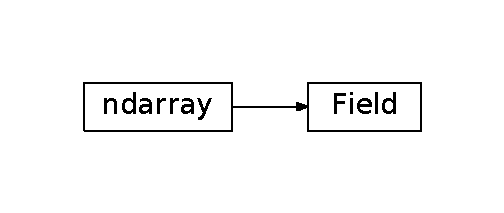
\includegraphics{inheritance-bd94d8d8d1fffd6b46be30171e123025249e6f21.pdf}
\phantomsection\label{api/climlab.domain:module-climlab.domain.field}\index{climlab.domain.field (module)}\index{Field (class in climlab.domain.field)}

\begin{fulllineitems}
\phantomsection\label{api/climlab.domain:climlab.domain.field.Field}\pysigline{\strong{class }\code{climlab.domain.field.}\bfcode{Field}}
Bases: \href{http://docs.scipy.org/doc/numpy/reference/generated/numpy.ndarray.html\#numpy.ndarray}{\code{numpy.ndarray}}

Custom class for climlab gridded quantities, called Field.

This class behaves exactly like \href{http://docs.scipy.org/doc/numpy/reference/generated/numpy.ndarray.html\#numpy.ndarray}{\code{numpy.ndarray}}
but every object has an attribute called \code{self.domain}
which is the domain associated with that field (e.g. state variables).

\textbf{Initialization parameters}

An instance of \code{Field} is initialized with the following 
arguments:
\begin{quote}\begin{description}
\item[{Parameters}] \leavevmode\begin{itemize}
\item {} 
\textbf{\texttt{input\_array}} (\href{http://docs.python.org/2.7/library/array.html\#module-array}{\emph{\texttt{array}}}) -- the array which the Field object should be 
initialized with

\item {} 
\textbf{\texttt{domain}} ({\hyperref[api/climlab.domain:climlab.domain.domain._Domain]{\emph{\code{\_Domain}}}} (\autopageref*{api/climlab.domain:climlab.domain.domain._Domain})) -- the domain associated with that field 
(e.g. state variables)

\end{itemize}

\end{description}\end{quote}

\textbf{Object attributes}

Following object attribute is generated during initialization:
\begin{quote}\begin{description}
\item[{Variables}] \leavevmode
{\hyperref[api/climlab.domain:module\string-climlab.domain.domain]{\emph{\textbf{\texttt{domain}}}}} (\autopageref*{api/climlab.domain:module-climlab.domain.domain}) ({\hyperref[api/climlab.domain:climlab.domain.domain._Domain]{\emph{\code{\_Domain}}}} (\autopageref*{api/climlab.domain:climlab.domain.domain._Domain})) -- the domain associated with that field 
(e.g. state variables)

\item[{Example}] \leavevmode
\begin{Verbatim}[commandchars=\\\{\}]
\PYG{g+gp}{\PYGZgt{}\PYGZgt{}\PYGZgt{} }\PYG{k+kn}{import} \PYG{n+nn}{climlab}
\PYG{g+gp}{\PYGZgt{}\PYGZgt{}\PYGZgt{} }\PYG{k+kn}{import} \PYG{n+nn}{numpy} \PYG{k+kn}{as} \PYG{n+nn}{np}
\PYG{g+gp}{\PYGZgt{}\PYGZgt{}\PYGZgt{} }\PYG{k+kn}{from} \PYG{n+nn}{climlab} \PYG{k+kn}{import} \PYG{n}{domain}
\PYG{g+gp}{\PYGZgt{}\PYGZgt{}\PYGZgt{} }\PYG{k+kn}{from} \PYG{n+nn}{climlab.domain} \PYG{k+kn}{import} \PYG{n}{field}

\PYG{g+gp}{\PYGZgt{}\PYGZgt{}\PYGZgt{} }\PYG{c+c1}{\PYGZsh{} distribution of state}
\PYG{g+gp}{\PYGZgt{}\PYGZgt{}\PYGZgt{} }\PYG{n}{distr} \PYG{o}{=} \PYG{n}{np}\PYG{o}{.}\PYG{n}{linspace}\PYG{p}{(}\PYG{l+m+mf}{0.}\PYG{p}{,} \PYG{l+m+mf}{10.}\PYG{p}{,} \PYG{l+m+mi}{30}\PYG{p}{)}
\PYG{g+gp}{\PYGZgt{}\PYGZgt{}\PYGZgt{} }\PYG{c+c1}{\PYGZsh{} domain creation}
\PYG{g+gp}{\PYGZgt{}\PYGZgt{}\PYGZgt{} }\PYG{n}{sfc}\PYG{p}{,} \PYG{n}{atm} \PYG{o}{=} \PYG{n}{domain}\PYG{o}{.}\PYG{n}{single\PYGZus{}column}\PYG{p}{(}\PYG{p}{)}
\PYG{g+gp}{\PYGZgt{}\PYGZgt{}\PYGZgt{} }\PYG{c+c1}{\PYGZsh{} build state of type Field}
\PYG{g+gp}{\PYGZgt{}\PYGZgt{}\PYGZgt{} }\PYG{n}{s} \PYG{o}{=} \PYG{n}{field}\PYG{o}{.}\PYG{n}{Field}\PYG{p}{(}\PYG{n}{distr}\PYG{p}{,} \PYG{n}{domain}\PYG{o}{=}\PYG{n}{atm}\PYG{p}{)}

\PYG{g+gp}{\PYGZgt{}\PYGZgt{}\PYGZgt{} }\PYG{k}{print} \PYG{n}{s}
\PYG{g+go}{[  0.           0.34482759   0.68965517   1.03448276   1.37931034}
\PYG{g+go}{   1.72413793   2.06896552   2.4137931    2.75862069   3.10344828}
\PYG{g+go}{   3.44827586   3.79310345   4.13793103   4.48275862   4.82758621}
\PYG{g+go}{   5.17241379   5.51724138   5.86206897   6.20689655   6.55172414}
\PYG{g+go}{   6.89655172   7.24137931   7.5862069    7.93103448   8.27586207}
\PYG{g+go}{   8.62068966   8.96551724   9.31034483   9.65517241  10.        ]}
\PYG{g+go}{   }
\PYG{g+gp}{\PYGZgt{}\PYGZgt{}\PYGZgt{} }\PYG{k}{print} \PYG{n}{s}\PYG{o}{.}\PYG{n}{domain}
\PYG{g+go}{climlab Domain object with domain\PYGZus{}type=atm and shape=(30,)}

\PYG{g+gp}{\PYGZgt{}\PYGZgt{}\PYGZgt{} }\PYG{c+c1}{\PYGZsh{} can slice this and it preserves the domain}
\PYG{g+gp}{\PYGZgt{}\PYGZgt{}\PYGZgt{} }\PYG{c+c1}{\PYGZsh{}  a more full\PYGZhy{}featured implementation would have intelligent}
\PYG{g+gp}{\PYGZgt{}\PYGZgt{}\PYGZgt{} }\PYG{c+c1}{\PYGZsh{}  slicing like in iris}
\PYG{g+gp}{\PYGZgt{}\PYGZgt{}\PYGZgt{} }\PYG{n}{s}\PYG{o}{.}\PYG{n}{shape} \PYG{o}{==} \PYG{n}{s}\PYG{o}{.}\PYG{n}{domain}\PYG{o}{.}\PYG{n}{shape}
\PYG{g+go}{True}
\PYG{g+gp}{\PYGZgt{}\PYGZgt{}\PYGZgt{} }\PYG{n}{s}\PYG{p}{[}\PYG{p}{:}\PYG{l+m+mi}{1}\PYG{p}{]}\PYG{o}{.}\PYG{n}{shape} \PYG{o}{==} \PYG{n}{s}\PYG{p}{[}\PYG{p}{:}\PYG{l+m+mi}{1}\PYG{p}{]}\PYG{o}{.}\PYG{n}{domain}\PYG{o}{.}\PYG{n}{shape}
\PYG{g+go}{False}

\PYG{g+gp}{\PYGZgt{}\PYGZgt{}\PYGZgt{} }\PYG{c+c1}{\PYGZsh{}  But some things work very well. E.g. new field creation:}
\PYG{g+gp}{\PYGZgt{}\PYGZgt{}\PYGZgt{} }\PYG{n}{s2} \PYG{o}{=} \PYG{n}{np}\PYG{o}{.}\PYG{n}{zeros\PYGZus{}like}\PYG{p}{(}\PYG{n}{s}\PYG{p}{)}

\PYG{g+gp}{\PYGZgt{}\PYGZgt{}\PYGZgt{} }\PYG{k}{print} \PYG{n}{s2}
\PYG{g+go}{[ 0.  0.  0.  0.  0.  0.  0.  0.  0.  0.  0.  0.  0.  0.  0.  0.  0.  0.}
\PYG{g+go}{  0.  0.  0.  0.  0.  0.  0.  0.  0.  0.  0.  0.]}
\PYG{g+go}{  }
\PYG{g+gp}{\PYGZgt{}\PYGZgt{}\PYGZgt{} }\PYG{k}{print} \PYG{n}{s2}\PYG{o}{.}\PYG{n}{domain}  
\PYG{g+go}{climlab Domain object with domain\PYGZus{}type=atm and shape=(30,)  }
\end{Verbatim}

\end{description}\end{quote}

\end{fulllineitems}

\index{global\_mean() (in module climlab.domain.field)}

\begin{fulllineitems}
\phantomsection\label{api/climlab.domain:climlab.domain.field.global_mean}\pysiglinewithargsret{\code{climlab.domain.field.}\bfcode{global\_mean}}{\emph{field}}{}
Calculates the latitude weighted global mean of a field 
with latitude dependence.
\begin{quote}\begin{description}
\item[{Parameters}] \leavevmode
\textbf{\texttt{field}} ({\hyperref[api/climlab.domain:climlab.domain.field.Field]{\emph{\emph{\texttt{Field}}}}} (\autopageref*{api/climlab.domain:climlab.domain.field.Field})) -- input field

\item[{Raises}] \leavevmode
\code{ValueError} if input field has no latitude axis

\item[{Returns}] \leavevmode
latitude weighted global mean of the field

\item[{Return type}] \leavevmode
\href{http://docs.python.org/2.7/library/functions.html\#float}{float}

\item[{Example}] \leavevmode
initial global mean temperature of EBM model:

\begin{Verbatim}[commandchars=\\\{\}]
\PYG{g+gp}{\PYGZgt{}\PYGZgt{}\PYGZgt{} }\PYG{k+kn}{import} \PYG{n+nn}{climlab}
\PYG{g+gp}{\PYGZgt{}\PYGZgt{}\PYGZgt{} }\PYG{k+kn}{from} \PYG{n+nn}{climlab.domain.field} \PYG{k+kn}{import} \PYG{n}{global\PYGZus{}mean}

\PYG{g+gp}{\PYGZgt{}\PYGZgt{}\PYGZgt{} }\PYG{n}{model} \PYG{o}{=} \PYG{n}{climlab}\PYG{o}{.}\PYG{n}{EBM}\PYG{p}{(}\PYG{p}{)}

\PYG{g+gp}{\PYGZgt{}\PYGZgt{}\PYGZgt{} }\PYG{n}{global\PYGZus{}mean}\PYG{p}{(}\PYG{n}{model}\PYG{o}{.}\PYG{n}{Ts}\PYG{p}{)}
\PYG{g+go}{Field(11.997968598413685)}
\end{Verbatim}

\end{description}\end{quote}

\end{fulllineitems}



\subsubsection{climlab.domain.initial module}
\label{api/climlab.domain:climlab-domain-initial-module}\label{api/climlab.domain:module-climlab.domain.initial}\index{climlab.domain.initial (module)}
Convenience routines for setting up initial conditions.
\index{column\_state() (in module climlab.domain.initial)}

\begin{fulllineitems}
\phantomsection\label{api/climlab.domain:climlab.domain.initial.column_state}\pysiglinewithargsret{\code{climlab.domain.initial.}\bfcode{column\_state}}{\emph{num\_lev=30}, \emph{num\_lat=1}, \emph{lev=None}, \emph{lat=None}, \emph{water\_depth=1.0}}{}
Sets up a state variable dictionary consisting of temperatures
for atmospheric column (\code{Tatm}) and surface mixed layer (\code{Ts}).

Surface temperature is always 288 K. Atmospheric temperature is initialized 
between 278 K at lowest altitude and 200 at top of atmosphere according to
the number of levels given.

\textbf{Function-call arguments}
\begin{quote}\begin{description}
\item[{Parameters}] \leavevmode\begin{itemize}
\item {} 
\textbf{\texttt{num\_lev}} (\href{http://docs.python.org/2.7/library/functions.html\#int}{\emph{\texttt{int}}}) -- number of pressure levels
(evenly spaced from surface to top of atmosphere) 
{[}default: 30{]}

\item {} 
\textbf{\texttt{num\_lat}} (\href{http://docs.python.org/2.7/library/functions.html\#int}{\emph{\texttt{int}}}) -- number of latitude points on the axis
{[}default: 1{]}

\item {} 
\textbf{\texttt{lev}} ({\hyperref[api/climlab.domain:climlab.domain.axis.Axis]{\emph{\code{Axis}}}} (\autopageref*{api/climlab.domain:climlab.domain.axis.Axis}) 
or pressure array) -- specification for height axis (optional)

\item {} 
\textbf{\texttt{lat}} (\href{http://docs.python.org/2.7/library/array.html\#module-array}{\emph{\texttt{array}}}) -- size of array determines dimension of latitude
(optional)

\item {} 
\textbf{\texttt{water\_depth}} (\href{http://docs.python.org/2.7/library/functions.html\#float}{\emph{\texttt{float}}}) -- \emph{irrelevant}

\end{itemize}

\item[{Returns}] \leavevmode
dictionary with two temperature 
{\hyperref[api/climlab.domain:climlab.domain.field.Field]{\emph{\code{Field}}}} (\autopageref*{api/climlab.domain:climlab.domain.field.Field}) 
for atmospheric column \code{Tatm} and 
surface mixed layer \code{Ts}

\item[{Return type}] \leavevmode
\href{http://docs.python.org/2.7/library/stdtypes.html\#dict}{dict}

\item[{Example}] \leavevmode
\begin{Verbatim}[commandchars=\\\{\}]
\PYG{g+gp}{\PYGZgt{}\PYGZgt{}\PYGZgt{} }\PYG{k+kn}{from} \PYG{n+nn}{climlab.domain} \PYG{k+kn}{import} \PYG{n}{initial}
\PYG{g+gp}{\PYGZgt{}\PYGZgt{}\PYGZgt{} }\PYG{n}{T\PYGZus{}dict} \PYG{o}{=} \PYG{n}{initial}\PYG{o}{.}\PYG{n}{column\PYGZus{}state}\PYG{p}{(}\PYG{p}{)}

\PYG{g+gp}{\PYGZgt{}\PYGZgt{}\PYGZgt{} }\PYG{k}{print} \PYG{n}{T\PYGZus{}dict}
\PYG{g+go}{\PYGZob{}\PYGZsq{}Tatm\PYGZsq{}: Field([ 200.        ,  202.68965517,  205.37931034,  208.06896552,}
\PYG{g+go}{        210.75862069,  213.44827586,  216.13793103,  218.82758621,}
\PYG{g+go}{        221.51724138,  224.20689655,  226.89655172,  229.5862069 ,}
\PYG{g+go}{        232.27586207,  234.96551724,  237.65517241,  240.34482759,}
\PYG{g+go}{        243.03448276,  245.72413793,  248.4137931 ,  251.10344828,}
\PYG{g+go}{        253.79310345,  256.48275862,  259.17241379,  261.86206897,}
\PYG{g+go}{        264.55172414,  267.24137931,  269.93103448,  272.62068966,}
\PYG{g+go}{        275.31034483,  278.        ]), \PYGZsq{}Ts\PYGZsq{}: Field([ 288.])\PYGZcb{}}
\end{Verbatim}

\end{description}\end{quote}

\end{fulllineitems}

\index{surface\_state() (in module climlab.domain.initial)}

\begin{fulllineitems}
\phantomsection\label{api/climlab.domain:climlab.domain.initial.surface_state}\pysiglinewithargsret{\code{climlab.domain.initial.}\bfcode{surface\_state}}{\emph{num\_lat=90}, \emph{water\_depth=10.0}, \emph{T0=12.0}, \emph{T2=-40.0}}{}
Sets up a state variable dictionary for a zonal-mean surface model
(e.g. basic EBM).

Returns a single state variable \emph{Ts}, the temperature of the surface 
mixed layer, initialized by a basic temperature and the second Legendre
polynomial.

\textbf{Function-call arguments}
\begin{quote}\begin{description}
\item[{Parameters}] \leavevmode\begin{itemize}
\item {} 
\textbf{\texttt{num\_lat}} (\href{http://docs.python.org/2.7/library/functions.html\#int}{\emph{\texttt{int}}}) -- number of latitude points on the axis
{[}default: 90{]}

\item {} 
\textbf{\texttt{water\_depth}} (\href{http://docs.python.org/2.7/library/functions.html\#float}{\emph{\texttt{float}}}) -- \emph{irrelevant}

\item {} 
\textbf{\texttt{T0}} (\href{http://docs.python.org/2.7/library/functions.html\#float}{\emph{\texttt{float}}}) -- 
base value for initial temperature
\begin{itemize}
\item {} 
unit \(^{\circ} \textrm{C}\)

\item {} 
default value: \code{12}

\end{itemize}


\item {} 
\textbf{\texttt{T2}} (\href{http://docs.python.org/2.7/library/functions.html\#float}{\emph{\texttt{float}}}) -- 
factor for 2nd Legendre polynomial 
{\hyperref[api/climlab.utils:climlab.utils.legendre.P2]{\emph{\code{P2}}}} (\autopageref*{api/climlab.utils:climlab.utils.legendre.P2}) 
to calculate initial temperature
\begin{itemize}
\item {} 
unit: dimensionless

\item {} 
default value: \code{-40}

\end{itemize}


\end{itemize}

\item[{Returns}] \leavevmode
dictionary with temperature 
{\hyperref[api/climlab.domain:climlab.domain.field.Field]{\emph{\code{Field}}}} (\autopageref*{api/climlab.domain:climlab.domain.field.Field}) 
for surface mixed layer \code{Ts}

\item[{Return type}] \leavevmode
\href{http://docs.python.org/2.7/library/stdtypes.html\#dict}{dict}

\item[{Example}] \leavevmode
\begin{Verbatim}[commandchars=\\\{\}]
\PYG{g+gp}{\PYGZgt{}\PYGZgt{}\PYGZgt{} }\PYG{k+kn}{from} \PYG{n+nn}{climlab.domain} \PYG{k+kn}{import} \PYG{n}{initial}
\PYG{g+gp}{\PYGZgt{}\PYGZgt{}\PYGZgt{} }\PYG{k+kn}{import} \PYG{n+nn}{numpy} \PYG{k+kn}{as} \PYG{n+nn}{np}

\PYG{g+gp}{\PYGZgt{}\PYGZgt{}\PYGZgt{} }\PYG{n}{T\PYGZus{}dict} \PYG{o}{=} \PYG{n}{initial}\PYG{o}{.}\PYG{n}{surface\PYGZus{}state}\PYG{p}{(}\PYG{n}{num\PYGZus{}lat}\PYG{o}{=}\PYG{l+m+mi}{36}\PYG{p}{)}

\PYG{g+gp}{\PYGZgt{}\PYGZgt{}\PYGZgt{} }\PYG{k}{print} \PYG{n}{np}\PYG{o}{.}\PYG{n}{squeeze}\PYG{p}{(}\PYG{n}{T\PYGZus{}dict}\PYG{p}{[}\PYG{l+s+s1}{\PYGZsq{}}\PYG{l+s+s1}{Ts}\PYG{l+s+s1}{\PYGZsq{}}\PYG{p}{]}\PYG{p}{)}
\PYG{g+go}{[\PYGZhy{}27.88584094 \PYGZhy{}26.97777479 \PYGZhy{}25.18923361 \PYGZhy{}22.57456133 \PYGZhy{}19.21320344}
\PYG{g+go}{ \PYGZhy{}15.20729309 \PYGZhy{}10.67854785  \PYGZhy{}5.76457135  \PYGZhy{}0.61467228   4.61467228}
\PYG{g+go}{   9.76457135  14.67854785  19.20729309  23.21320344  26.57456133}
\PYG{g+go}{  29.18923361  30.97777479  31.88584094  31.88584094  30.97777479}
\PYG{g+go}{  29.18923361  26.57456133  23.21320344  19.20729309  14.67854785}
\PYG{g+go}{   9.76457135   4.61467228  \PYGZhy{}0.61467228  \PYGZhy{}5.76457135 \PYGZhy{}10.67854785}
\PYG{g+go}{ \PYGZhy{}15.20729309 \PYGZhy{}19.21320344 \PYGZhy{}22.57456133 \PYGZhy{}25.18923361 \PYGZhy{}26.97777479}
\PYG{g+go}{ \PYGZhy{}27.88584094]}
\end{Verbatim}

\end{description}\end{quote}

\end{fulllineitems}



\subsection{climlab.dynamics package}
\label{api/climlab.dynamics:climlab-dynamics-package}\label{api/climlab.dynamics::doc}

\subsubsection{climlab.dynamics.budyko\_transport module}
\label{api/climlab.dynamics:climlab-dynamics-budyko-transport-module}
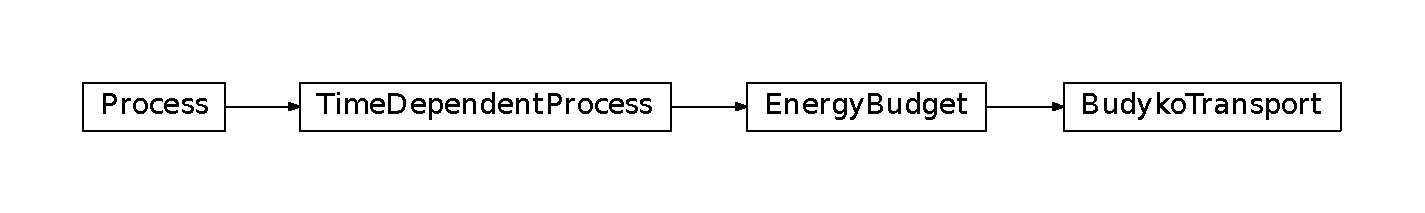
\includegraphics{inheritance-598e25126bb3e29c3e0d23aa40ddae14047c92c2.pdf}
\phantomsection\label{api/climlab.dynamics:module-climlab.dynamics.budyko_transport}\index{climlab.dynamics.budyko\_transport (module)}\index{BudykoTransport (class in climlab.dynamics.budyko\_transport)}

\begin{fulllineitems}
\phantomsection\label{api/climlab.dynamics:climlab.dynamics.budyko_transport.BudykoTransport}\pysiglinewithargsret{\strong{class }\code{climlab.dynamics.budyko\_transport.}\bfcode{BudykoTransport}}{\emph{b=3.81}, \emph{**kwargs}}{}
Bases: {\hyperref[api/climlab.process:climlab.process.energy_budget.EnergyBudget]{\emph{\code{climlab.process.energy\_budget.EnergyBudget}}}} (\autopageref*{api/climlab.process:climlab.process.energy_budget.EnergyBudget})

calculates the 1 dimensional heat transport as the difference 
between the local temperature and the global mean temperature.
\begin{quote}\begin{description}
\item[{Parameters}] \leavevmode
\textbf{\texttt{b}} (\href{http://docs.python.org/2.7/library/functions.html\#float}{\emph{\texttt{float}}}) -- 
budyko transport parameter
\begin{itemize}
\item {} 
unit: \(\textrm{W} / \left( \textrm{m}^2 \ ^{\circ} \textrm{C} \right)\)

\item {} 
default value: \code{3.81}

\end{itemize}


\end{description}\end{quote}

As BudykoTransport is a {\hyperref[api/climlab.process:climlab.process.process.Process]{\emph{\code{Process}}}} (\autopageref*{api/climlab.process:climlab.process.process.Process}) it needs
a state do be defined on. See example for details.

\textbf{Computation Details:}

In a global Energy Balance Model
\begin{gather}
\begin{split}C \frac{dT}{dt} = R\downarrow - R\uparrow - H\end{split}\notag
\end{gather}
with model state \(T\), the energy transport term \(H\) 
can be described as
\begin{gather}
\begin{split}H = b [T - \bar{T}]\end{split}\notag
\end{gather}
where \(T\) is a vector of the model temperature and \(\bar{T}\)
describes the mean value of \(T\).

For further information see {[}Budyko\_1969{]}.
\begin{quote}\begin{description}
\item[{Example}] \leavevmode
Budyko Transport as a standalone process:

\begin{Verbatim}[commandchars=\\\{\}]
\PYG{k+kn}{import} \PYG{n+nn}{climlab}
\PYG{k+kn}{from} \PYG{n+nn}{climlab.dynamics.budyko\PYGZus{}transport} \PYG{k+kn}{import} \PYG{n}{BudykoTransport}
\PYG{k+kn}{from} \PYG{n+nn}{climlab} \PYG{k+kn}{import} \PYG{n}{domain}
\PYG{k+kn}{from} \PYG{n+nn}{climlab.domain} \PYG{k+kn}{import} \PYG{n}{field}
\PYG{k+kn}{from} \PYG{n+nn}{climlab.utils.legendre} \PYG{k+kn}{import} \PYG{n}{P2}
\PYG{k+kn}{import} \PYG{n+nn}{numpy} \PYG{k+kn}{as} \PYG{n+nn}{np}
\PYG{k+kn}{import} \PYG{n+nn}{matplotlib.pyplot} \PYG{k+kn}{as} \PYG{n+nn}{plt}

\PYG{c+c1}{\PYGZsh{} create domain}
\PYG{n}{sfc} \PYG{o}{=} \PYG{n}{domain}\PYG{o}{.}\PYG{n}{zonal\PYGZus{}mean\PYGZus{}surface}\PYG{p}{(}\PYG{n}{num\PYGZus{}lat} \PYG{o}{=} \PYG{l+m+mi}{36}\PYG{p}{)}

\PYG{n}{lat} \PYG{o}{=} \PYG{n}{sfc}\PYG{o}{.}\PYG{n}{lat}\PYG{o}{.}\PYG{n}{points}
\PYG{n}{lat\PYGZus{}rad} \PYG{o}{=} \PYG{n}{np}\PYG{o}{.}\PYG{n}{deg2rad}\PYG{p}{(}\PYG{n}{lat}\PYG{p}{)}

\PYG{c+c1}{\PYGZsh{} define initial temperature distribution}
\PYG{n}{T0} \PYG{o}{=} \PYG{l+m+mf}{15.}
\PYG{n}{T2} \PYG{o}{=} \PYG{o}{\PYGZhy{}}\PYG{l+m+mf}{20.}
\PYG{n}{Ts} \PYG{o}{=} \PYG{n}{field}\PYG{o}{.}\PYG{n}{Field}\PYG{p}{(}\PYG{n}{T0} \PYG{o}{+} \PYG{n}{T2} \PYG{o}{*} \PYG{n}{P2}\PYG{p}{(}\PYG{n}{np}\PYG{o}{.}\PYG{n}{sin}\PYG{p}{(}\PYG{n}{lat\PYGZus{}rad}\PYG{p}{)}\PYG{p}{)}\PYG{p}{,} \PYG{n}{domain}\PYG{o}{=}\PYG{n}{sfc}\PYG{p}{)}

\PYG{c+c1}{\PYGZsh{} create BudykoTransport process}
\PYG{n}{budyko\PYGZus{}transp} \PYG{o}{=} \PYG{n}{BudykoTransport}\PYG{p}{(}\PYG{n}{state}\PYG{o}{=}\PYG{n}{Ts}\PYG{p}{)}

\PYG{c+c1}{\PYGZsh{}\PYGZsh{}\PYGZsh{} Integrate \PYGZam{} Plot \PYGZsh{}\PYGZsh{}\PYGZsh{}}

\PYG{n}{fig} \PYG{o}{=} \PYG{n}{plt}\PYG{o}{.}\PYG{n}{figure}\PYG{p}{(} \PYG{n}{figsize}\PYG{o}{=}\PYG{p}{(}\PYG{l+m+mi}{6}\PYG{p}{,}\PYG{l+m+mi}{4}\PYG{p}{)}\PYG{p}{)}
\PYG{n}{ax} \PYG{o}{=} \PYG{n}{fig}\PYG{o}{.}\PYG{n}{add\PYGZus{}subplot}\PYG{p}{(}\PYG{l+m+mi}{111}\PYG{p}{)}

\PYG{k}{for} \PYG{n}{i} \PYG{o+ow}{in} \PYG{n}{np}\PYG{o}{.}\PYG{n}{arange}\PYG{p}{(}\PYG{l+m+mi}{0}\PYG{p}{,}\PYG{l+m+mi}{3}\PYG{p}{,}\PYG{l+m+mi}{1}\PYG{p}{)}\PYG{p}{:}
    \PYG{n}{ax}\PYG{o}{.}\PYG{n}{plot}\PYG{p}{(}\PYG{n}{lat}\PYG{p}{,} \PYG{n}{budyko\PYGZus{}transp}\PYG{o}{.}\PYG{n}{default}\PYG{p}{,} \PYG{n}{label}\PYG{o}{=}\PYG{l+s+s1}{\PYGZsq{}}\PYG{l+s+s1}{day }\PYG{l+s+si}{\PYGZpc{}s}\PYG{l+s+s1}{\PYGZsq{}} \PYG{o}{\PYGZpc{}} \PYG{p}{(}\PYG{n}{i}\PYG{o}{*}\PYG{l+m+mi}{40}\PYG{p}{)}\PYG{p}{)}
    \PYG{n}{budyko\PYGZus{}transp}\PYG{o}{.}\PYG{n}{integrate\PYGZus{}days}\PYG{p}{(}\PYG{l+m+mf}{40.}\PYG{p}{)}

\PYG{n}{ax}\PYG{o}{.}\PYG{n}{set\PYGZus{}title}\PYG{p}{(}\PYG{l+s+s1}{\PYGZsq{}}\PYG{l+s+s1}{Standalone Budyko Transport}\PYG{l+s+s1}{\PYGZsq{}}\PYG{p}{)}
\PYG{n}{ax}\PYG{o}{.}\PYG{n}{set\PYGZus{}xlabel}\PYG{p}{(}\PYG{l+s+s1}{\PYGZsq{}}\PYG{l+s+s1}{latitude}\PYG{l+s+s1}{\PYGZsq{}}\PYG{p}{)}
\PYG{n}{ax}\PYG{o}{.}\PYG{n}{set\PYGZus{}xticks}\PYG{p}{(}\PYG{p}{[}\PYG{o}{\PYGZhy{}}\PYG{l+m+mi}{90}\PYG{p}{,}\PYG{o}{\PYGZhy{}}\PYG{l+m+mi}{60}\PYG{p}{,}\PYG{o}{\PYGZhy{}}\PYG{l+m+mi}{30}\PYG{p}{,}\PYG{l+m+mi}{0}\PYG{p}{,}\PYG{l+m+mi}{30}\PYG{p}{,}\PYG{l+m+mi}{60}\PYG{p}{,}\PYG{l+m+mi}{90}\PYG{p}{]}\PYG{p}{)}
\PYG{n}{ax}\PYG{o}{.}\PYG{n}{set\PYGZus{}ylabel}\PYG{p}{(}\PYG{l+s+s1}{\PYGZsq{}}\PYG{l+s+s1}{temperature (\PYGZdl{}\PYGZca{}\PYGZob{}}\PYG{l+s+s1}{\PYGZbs{}}\PYG{l+s+s1}{circ\PYGZcb{}\PYGZdl{}C)}\PYG{l+s+s1}{\PYGZsq{}}\PYG{p}{)}
\PYG{n}{ax}\PYG{o}{.}\PYG{n}{legend}\PYG{p}{(}\PYG{n}{loc}\PYG{o}{=}\PYG{l+s+s1}{\PYGZsq{}}\PYG{l+s+s1}{best}\PYG{l+s+s1}{\PYGZsq{}}\PYG{p}{)}
\PYG{n}{plt}\PYG{o}{.}\PYG{n}{show}\PYG{p}{(}\PYG{p}{)}
\end{Verbatim}

\includegraphics{{example_budyko_transport}.pdf}

\end{description}\end{quote}
\index{b (climlab.dynamics.budyko\_transport.BudykoTransport attribute)}

\begin{fulllineitems}
\phantomsection\label{api/climlab.dynamics:climlab.dynamics.budyko_transport.BudykoTransport.b}\pysigline{\bfcode{b}}
the budyko transport parameter in unit 
\(\frac{\textrm{W}}{\textrm{m}^2 \textrm{K}}\)
\begin{quote}\begin{description}
\item[{Getter}] \leavevmode
returns the budyko transport parameter

\item[{Setter}] \leavevmode
sets the budyko transport parameter

\item[{Type}] \leavevmode
float

\end{description}\end{quote}

\end{fulllineitems}


\end{fulllineitems}



\subsubsection{climlab.dynamics.diffusion module}
\label{api/climlab.dynamics:climlab-dynamics-diffusion-module}
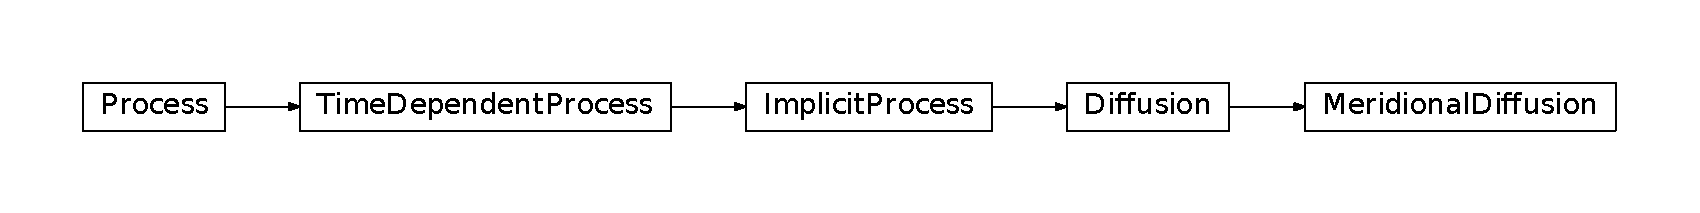
\includegraphics{inheritance-804892074707de77374c9484dbf91ce4dddd70eb.pdf}
\phantomsection\label{api/climlab.dynamics:module-climlab.dynamics.diffusion}\index{climlab.dynamics.diffusion (module)}\index{Diffusion (class in climlab.dynamics.diffusion)}

\begin{fulllineitems}
\phantomsection\label{api/climlab.dynamics:climlab.dynamics.diffusion.Diffusion}\pysiglinewithargsret{\strong{class }\code{climlab.dynamics.diffusion.}\bfcode{Diffusion}}{\emph{K=None}, \emph{diffusion\_axis=None}, \emph{use\_banded\_solver=False}, \emph{**kwargs}}{}
Bases: {\hyperref[api/climlab.process:climlab.process.implicit.ImplicitProcess]{\emph{\code{climlab.process.implicit.ImplicitProcess}}}} (\autopageref*{api/climlab.process:climlab.process.implicit.ImplicitProcess})

A parent class for one dimensional implicit diffusion modules.

Solves the one dimensional heat equation
\begin{gather}
\begin{split}\frac{dT}{dt} = \frac{d}{dy} \left[ K \cdot \frac{dT}{dy} \right]\end{split}\notag
\end{gather}
\textbf{Initialization parameters}
\begin{quote}\begin{description}
\item[{Parameters}] \leavevmode\begin{itemize}
\item {} 
\textbf{\texttt{K}} (\href{http://docs.python.org/2.7/library/functions.html\#float}{\emph{\texttt{float}}}) -- the diffusivity parameter in units of 
\(\frac{[\textrm{length}]^2}{\textrm{time}}\)
where length is the unit of the spatial axis
on which the diffusion is occuring.

\item {} 
\textbf{\texttt{diffusion\_axis}} (\href{http://docs.python.org/2.7/library/functions.html\#str}{\emph{\texttt{str}}}) -- dictionary key for axis on which the 
diffusion is occuring in process's domain
axes dictionary

\item {} 
\textbf{\texttt{use\_banded\_solver}} (\href{http://docs.python.org/2.7/library/functions.html\#bool}{\emph{\texttt{bool}}}) -- input flag, whether to use 
\href{http://docs.scipy.org/doc/scipy/reference/generated/scipy.linalg.solve\_banded.html\#scipy.linalg.solve\_banded}{\code{scipy.linalg.solve\_banded()}}
instead of \href{http://docs.scipy.org/doc/numpy/reference/generated/numpy.linalg.solve.html\#numpy.linalg.solve}{\code{numpy.linalg.solve()}}
{[}default: False{]}

\end{itemize}

\end{description}\end{quote}

\begin{notice}{note}{Note:}
The banded solver \href{http://docs.scipy.org/doc/scipy/reference/generated/scipy.linalg.solve\_banded.html\#scipy.linalg.solve\_banded}{\code{scipy.linalg.solve\_banded()}} is faster than 
\href{http://docs.scipy.org/doc/numpy/reference/generated/numpy.linalg.solve.html\#numpy.linalg.solve}{\code{numpy.linalg.solve()}} but only works for one dimensional diffusion.
\end{notice}

\textbf{Object attributes}

Additional to the parent class 
{\hyperref[api/climlab.process:climlab.process.implicit.ImplicitProcess]{\emph{\code{ImplicitProcess}}}} (\autopageref*{api/climlab.process:climlab.process.implicit.ImplicitProcess})
following object attributes are generated or modified during initialization:
\begin{quote}\begin{description}
\item[{Variables}] \leavevmode\begin{itemize}
\item {} 
\textbf{\texttt{param}} (\href{http://docs.python.org/2.7/library/stdtypes.html\#dict}{\emph{\texttt{dict}}}) -- parameter dictionary is extended by 
diffusivity parameter K (unit:
\(\frac{[\textrm{length}]^2}{\textrm{time}}\))

\item {} 
\textbf{\texttt{use\_banded\_solver}} (\href{http://docs.python.org/2.7/library/functions.html\#bool}{\emph{\texttt{bool}}}) -- input flag specifying numerical solving 
method (given during initialization)

\item {} 
\textbf{\texttt{diffusion\_axis}} (\href{http://docs.python.org/2.7/library/functions.html\#str}{\emph{\texttt{str}}}) -- dictionary key for axis where diffusion 
is occuring: 
specified during initialization
or output of method 
{\hyperref[api/climlab.dynamics:climlab.dynamics.diffusion._guess_diffusion_axis]{\emph{\code{\_guess\_diffusion\_axis()}}}} (\autopageref*{api/climlab.dynamics:climlab.dynamics.diffusion._guess_diffusion_axis})

\item {} 
\textbf{\texttt{K\_dimensionless}} (\href{http://docs.python.org/2.7/library/array.html\#module-array}{\emph{\texttt{array}}}) -- diffusion parameter K multiplied by the 
timestep and divided by mean of diffusion 
axis delta in the power of two. Array has 
the size of diffusion axis bounds.
\(K_{\textrm{dimensionless}}[i]= K \frac{\Delta t}{ \left(\overline{\Delta \textrm{bounds}} \right)^2}\)

\item {} 
\textbf{\texttt{diffTriDiag}} (\href{http://docs.python.org/2.7/library/array.html\#module-array}{\emph{\texttt{array}}}) -- tridiagonal diffusion matrix made by
{\hyperref[api/climlab.dynamics:climlab.dynamics.diffusion._make_diffusion_matrix]{\emph{\code{\_make\_diffusion\_matrix()}}}} (\autopageref*{api/climlab.dynamics:climlab.dynamics.diffusion._make_diffusion_matrix}) with input
\code{self.K\_dimensionless}

\end{itemize}

\item[{Example}] \leavevmode
Here is an example showing implementation of a vertical diffusion.
It shows that a subprocess can work on just a subset of the parent process
state variables.
\begin{quote}

\begin{Verbatim}[commandchars=\\\{\}]
\PYG{k+kn}{import} \PYG{n+nn}{climlab}
\PYG{k+kn}{from} \PYG{n+nn}{climlab.dynamics.diffusion} \PYG{k+kn}{import} \PYG{n}{Diffusion}
\PYG{k+kn}{import} \PYG{n+nn}{matplotlib.pyplot} \PYG{k+kn}{as} \PYG{n+nn}{plt}

\PYG{n}{c} \PYG{o}{=} \PYG{n}{climlab}\PYG{o}{.}\PYG{n}{GreyRadiationModel}\PYG{p}{(}\PYG{p}{)}
\PYG{n}{K} \PYG{o}{=} \PYG{l+m+mf}{0.5}
\PYG{n}{d} \PYG{o}{=} \PYG{n}{Diffusion}\PYG{p}{(}\PYG{n}{K}\PYG{o}{=}\PYG{n}{K}\PYG{p}{,} \PYG{n}{state} \PYG{o}{=} \PYG{p}{\PYGZob{}}\PYG{l+s+s1}{\PYGZsq{}}\PYG{l+s+s1}{Tatm}\PYG{l+s+s1}{\PYGZsq{}}\PYG{p}{:}\PYG{n}{c}\PYG{o}{.}\PYG{n}{state}\PYG{p}{[}\PYG{l+s+s1}{\PYGZsq{}}\PYG{l+s+s1}{Tatm}\PYG{l+s+s1}{\PYGZsq{}}\PYG{p}{]}\PYG{p}{\PYGZcb{}}\PYG{p}{,} \PYG{o}{*}\PYG{o}{*}\PYG{n}{c}\PYG{o}{.}\PYG{n}{param}\PYG{p}{)}

\PYG{n}{c}\PYG{o}{.}\PYG{n}{add\PYGZus{}subprocess}\PYG{p}{(}\PYG{l+s+s1}{\PYGZsq{}}\PYG{l+s+s1}{diffusion}\PYG{l+s+s1}{\PYGZsq{}}\PYG{p}{,}\PYG{n}{d}\PYG{p}{)}

\PYG{c+c1}{\PYGZsh{}\PYGZsh{}\PYGZsh{} Integrate \PYGZam{} Plot \PYGZsh{}\PYGZsh{}\PYGZsh{}}

\PYG{n}{fig} \PYG{o}{=} \PYG{n}{plt}\PYG{o}{.}\PYG{n}{figure}\PYG{p}{(} \PYG{n}{figsize}\PYG{o}{=}\PYG{p}{(}\PYG{l+m+mi}{6}\PYG{p}{,}\PYG{l+m+mi}{4}\PYG{p}{)}\PYG{p}{)}
\PYG{n}{ax} \PYG{o}{=} \PYG{n}{fig}\PYG{o}{.}\PYG{n}{add\PYGZus{}subplot}\PYG{p}{(}\PYG{l+m+mi}{111}\PYG{p}{)}

\PYG{n}{ax}\PYG{o}{.}\PYG{n}{plot}\PYG{p}{(}\PYG{n}{c}\PYG{o}{.}\PYG{n}{lev}\PYG{p}{,} \PYG{n}{c}\PYG{o}{.}\PYG{n}{state}\PYG{p}{[}\PYG{l+s+s1}{\PYGZsq{}}\PYG{l+s+s1}{Tatm}\PYG{l+s+s1}{\PYGZsq{}}\PYG{p}{]}\PYG{p}{,} \PYG{n}{label}\PYG{o}{=}\PYG{l+s+s1}{\PYGZsq{}}\PYG{l+s+s1}{step 0}\PYG{l+s+s1}{\PYGZsq{}}\PYG{p}{)}
\PYG{n}{c}\PYG{o}{.}\PYG{n}{step\PYGZus{}forward}\PYG{p}{(}\PYG{p}{)}
\PYG{n}{ax}\PYG{o}{.}\PYG{n}{plot}\PYG{p}{(}\PYG{n}{c}\PYG{o}{.}\PYG{n}{lev}\PYG{p}{,} \PYG{n}{c}\PYG{o}{.}\PYG{n}{state}\PYG{p}{[}\PYG{l+s+s1}{\PYGZsq{}}\PYG{l+s+s1}{Tatm}\PYG{l+s+s1}{\PYGZsq{}}\PYG{p}{]}\PYG{p}{,} \PYG{n}{label}\PYG{o}{=}\PYG{l+s+s1}{\PYGZsq{}}\PYG{l+s+s1}{step 1}\PYG{l+s+s1}{\PYGZsq{}}\PYG{p}{)}

\PYG{n}{ax}\PYG{o}{.}\PYG{n}{invert\PYGZus{}xaxis}\PYG{p}{(}\PYG{p}{)}
\PYG{n}{ax}\PYG{o}{.}\PYG{n}{set\PYGZus{}title}\PYG{p}{(}\PYG{l+s+s1}{\PYGZsq{}}\PYG{l+s+s1}{Diffusion subprocess}\PYG{l+s+s1}{\PYGZsq{}}\PYG{p}{)}
\PYG{n}{ax}\PYG{o}{.}\PYG{n}{set\PYGZus{}xlabel}\PYG{p}{(}\PYG{l+s+s1}{\PYGZsq{}}\PYG{l+s+s1}{level (mb)}\PYG{l+s+s1}{\PYGZsq{}}\PYG{p}{)}
\PYG{c+c1}{\PYGZsh{}ax.set\PYGZus{}xticks([])}
\PYG{n}{ax}\PYG{o}{.}\PYG{n}{set\PYGZus{}ylabel}\PYG{p}{(}\PYG{l+s+s1}{\PYGZsq{}}\PYG{l+s+s1}{temperature (K)}\PYG{l+s+s1}{\PYGZsq{}}\PYG{p}{)}
\PYG{n}{ax}\PYG{o}{.}\PYG{n}{legend}\PYG{p}{(}\PYG{n}{loc}\PYG{o}{=}\PYG{l+s+s1}{\PYGZsq{}}\PYG{l+s+s1}{best}\PYG{l+s+s1}{\PYGZsq{}}\PYG{p}{)}
\PYG{n}{plt}\PYG{o}{.}\PYG{n}{show}\PYG{p}{(}\PYG{p}{)}
\end{Verbatim}

\includegraphics{{example_diffusion}.pdf}
\end{quote}

\end{description}\end{quote}
\index{\_implicit\_solver() (climlab.dynamics.diffusion.Diffusion method)}

\begin{fulllineitems}
\phantomsection\label{api/climlab.dynamics:climlab.dynamics.diffusion.Diffusion._implicit_solver}\pysiglinewithargsret{\bfcode{\_implicit\_solver}}{}{}
Invertes and solves the matrix problem for diffusion matrix 
and temperature T.

The method is called by the 
{\hyperref[api/climlab.process:climlab.process.implicit.ImplicitProcess._compute]{\emph{\code{\_compute()}}}} (\autopageref*{api/climlab.process:climlab.process.implicit.ImplicitProcess._compute}) function 
of the {\hyperref[api/climlab.process:climlab.process.implicit.ImplicitProcess]{\emph{\code{ImplicitProcess}}}} (\autopageref*{api/climlab.process:climlab.process.implicit.ImplicitProcess}) class and 
solves the matrix problem
\begin{gather}
\begin{split}A \cdot T_{\textrm{new}} = T_{\textrm{old}}\end{split}\notag
\end{gather}
for diffusion matrix A and corresponding temperatures. 
\(T_{\textrm{old}}\) is in this case the current state variable 
which already has been adjusted by the explicit processes. 
\(T_{\textrm{new}}\) is the new state of the variable. To
derive the temperature tendency of the diffusion process the adjustment 
has to be calculated and muliplied with the timestep which is done by
the {\hyperref[api/climlab.process:climlab.process.implicit.ImplicitProcess._compute]{\emph{\code{\_compute()}}}} (\autopageref*{api/climlab.process:climlab.process.implicit.ImplicitProcess._compute}) 
function of the {\hyperref[api/climlab.process:climlab.process.implicit.ImplicitProcess]{\emph{\code{ImplicitProcess}}}} (\autopageref*{api/climlab.process:climlab.process.implicit.ImplicitProcess}) 
class.

This method calculates the matrix inversion for every state variable
and calling either \code{solve\_implicit\_banded()} or 
\href{http://docs.scipy.org/doc/numpy/reference/generated/numpy.linalg.solve.html\#numpy.linalg.solve}{\code{numpy.linalg.solve()}} dependent on the flag 
\code{self.use\_banded\_solver}.
\begin{quote}\begin{description}
\item[{Variables}] \leavevmode\begin{itemize}
\item {} 
\textbf{\texttt{state}} (\href{http://docs.python.org/2.7/library/stdtypes.html\#dict}{\emph{\texttt{dict}}}) -- method uses current state variables
but does not modify them

\item {} 
\textbf{\texttt{use\_banded\_solver}} (\href{http://docs.python.org/2.7/library/functions.html\#bool}{\emph{\texttt{bool}}}) -- input flag whether to use 
{\hyperref[api/climlab.dynamics:climlab.dynamics.diffusion._solve_implicit_banded]{\emph{\code{\_solve\_implicit\_banded()}}}} (\autopageref*{api/climlab.dynamics:climlab.dynamics.diffusion._solve_implicit_banded}) or 
\href{http://docs.scipy.org/doc/numpy/reference/generated/numpy.linalg.solve.html\#numpy.linalg.solve}{\code{numpy.linalg.solve()}} to do 
the matrix inversion

\item {} 
\textbf{\texttt{diffTriDiag}} (\href{http://docs.python.org/2.7/library/array.html\#module-array}{\emph{\texttt{array}}}) -- the diffusion matrix which is given 
with the current state variable to 
the method solving the matrix problem

\end{itemize}

\end{description}\end{quote}

\end{fulllineitems}


\end{fulllineitems}

\index{MeridionalDiffusion (class in climlab.dynamics.diffusion)}

\begin{fulllineitems}
\phantomsection\label{api/climlab.dynamics:climlab.dynamics.diffusion.MeridionalDiffusion}\pysiglinewithargsret{\strong{class }\code{climlab.dynamics.diffusion.}\bfcode{MeridionalDiffusion}}{\emph{K=None}, \emph{**kwargs}}{}
Bases: {\hyperref[api/climlab.dynamics:climlab.dynamics.diffusion.Diffusion]{\emph{\code{climlab.dynamics.diffusion.Diffusion}}}} (\autopageref*{api/climlab.dynamics:climlab.dynamics.diffusion.Diffusion})

A parent class for Meridional diffusion processes.

Calculates the energy transport in a diffusion like process along the
temperature gradient:
\begin{quote}
\begin{quote}
\begin{gather}
\begin{split}H(\varphi) = \frac{D}{\cos \varphi}\frac{\partial}{\partial \varphi} \left( \cos\varphi \frac{\partial T(\varphi)}{\partial \varphi} \right)\end{split}\notag
\end{gather}\end{quote}

for an Energy Balance Model whose Energy Budget can be noted as:
\begin{gather}
\begin{split}C(\varphi) \frac{dT(\varphi)}{dt} = R\downarrow (\varphi) - R\uparrow (\varphi) + H(\varphi)\end{split}\notag
\end{gather}\end{quote}

\textbf{Initialization parameters}

An instance of \code{MeridionalDiffusion} is initialized with the following 
arguments:
\begin{quote}\begin{description}
\item[{Parameters}] \leavevmode
\textbf{\texttt{K}} (\href{http://docs.python.org/2.7/library/functions.html\#float}{\emph{\texttt{float}}}) -- diffusion parameter in units of \(1/s\)

\end{description}\end{quote}

\textbf{Object attributes}

Additional to the parent class {\hyperref[api/climlab.dynamics:climlab.dynamics.diffusion.Diffusion]{\emph{\code{Diffusion}}}} (\autopageref*{api/climlab.dynamics:climlab.dynamics.diffusion.Diffusion})
which is initialized with \code{diffusion\_axis='lat'}, following object 
attributes are modified during initialization:
\begin{quote}\begin{description}
\item[{Variables}] \leavevmode\begin{itemize}
\item {} 
\textbf{\texttt{K\_dimensionless}} (\href{http://docs.python.org/2.7/library/array.html\#module-array}{\emph{\texttt{array}}}) -- As K\_dimensionless has been computed like
\(K_{\textrm{dimensionless}}= K \frac{\Delta t}{(\Delta \textrm{bounds})^2}\)
with \(K\) in units \(1/s\), 
the \(\Delta (\textrm{bounds})\) have to
be converted from \code{deg} to \code{rad} to make 
the array actually dimensionless. 
This is done during initialiation.

\item {} 
\textbf{\texttt{diffTriDiag}} (\href{http://docs.python.org/2.7/library/array.html\#module-array}{\emph{\texttt{array}}}) -- the diffusion matrix is recomputed with
appropriate weights for the meridional case
by {\hyperref[api/climlab.dynamics:climlab.dynamics.diffusion._make_meridional_diffusion_matrix]{\emph{\code{\_make\_meridional\_diffusion\_matrix()}}}} (\autopageref*{api/climlab.dynamics:climlab.dynamics.diffusion._make_meridional_diffusion_matrix})

\end{itemize}

\item[{Example}] \leavevmode
Meridional Diffusion of temperature
as a stand-alone process:

\begin{Verbatim}[commandchars=\\\{\}]
\PYG{k+kn}{import} \PYG{n+nn}{numpy} \PYG{k+kn}{as} \PYG{n+nn}{np}
\PYG{k+kn}{import} \PYG{n+nn}{climlab}
\PYG{k+kn}{from} \PYG{n+nn}{climlab.dynamics.diffusion} \PYG{k+kn}{import} \PYG{n}{MeridionalDiffusion}
\PYG{k+kn}{from} \PYG{n+nn}{climlab.utils} \PYG{k+kn}{import} \PYG{n}{legendre}

\PYG{n}{sfc} \PYG{o}{=} \PYG{n}{climlab}\PYG{o}{.}\PYG{n}{domain}\PYG{o}{.}\PYG{n}{zonal\PYGZus{}mean\PYGZus{}surface}\PYG{p}{(}\PYG{n}{num\PYGZus{}lat}\PYG{o}{=}\PYG{l+m+mi}{90}\PYG{p}{,} \PYG{n}{water\PYGZus{}depth}\PYG{o}{=}\PYG{l+m+mf}{10.}\PYG{p}{)}
\PYG{n}{lat} \PYG{o}{=} \PYG{n}{sfc}\PYG{o}{.}\PYG{n}{lat}\PYG{o}{.}\PYG{n}{points}
\PYG{n}{initial} \PYG{o}{=} \PYG{l+m+mf}{12.} \PYG{o}{\PYGZhy{}} \PYG{l+m+mf}{40.} \PYG{o}{*} \PYG{n}{legendre}\PYG{o}{.}\PYG{n}{P2}\PYG{p}{(}\PYG{n}{np}\PYG{o}{.}\PYG{n}{sin}\PYG{p}{(}\PYG{n}{np}\PYG{o}{.}\PYG{n}{deg2rad}\PYG{p}{(}\PYG{n}{lat}\PYG{p}{)}\PYG{p}{)}\PYG{p}{)}

\PYG{c+c1}{\PYGZsh{} make a copy of initial so that it remains unmodified}
\PYG{n}{Ts} \PYG{o}{=} \PYG{n}{climlab}\PYG{o}{.}\PYG{n}{Field}\PYG{p}{(}\PYG{n}{np}\PYG{o}{.}\PYG{n}{array}\PYG{p}{(}\PYG{n}{initial}\PYG{p}{)}\PYG{p}{,} \PYG{n}{domain}\PYG{o}{=}\PYG{n}{sfc}\PYG{p}{)}

\PYG{c+c1}{\PYGZsh{} thermal diffusivity in W/m**2/degC}
\PYG{n}{D} \PYG{o}{=} \PYG{l+m+mf}{0.55}

\PYG{c+c1}{\PYGZsh{} meridional diffusivity in 1/s}
\PYG{n}{K} \PYG{o}{=} \PYG{n}{D} \PYG{o}{/} \PYG{n}{sfc}\PYG{o}{.}\PYG{n}{heat\PYGZus{}capacity}
\PYG{n}{d} \PYG{o}{=} \PYG{n}{MeridionalDiffusion}\PYG{p}{(}\PYG{n}{state}\PYG{o}{=}\PYG{n}{Ts}\PYG{p}{,} \PYG{n}{K}\PYG{o}{=}\PYG{n}{K}\PYG{p}{)}

\PYG{n}{d}\PYG{o}{.}\PYG{n}{integrate\PYGZus{}years}\PYG{p}{(}\PYG{l+m+mf}{1.}\PYG{p}{)}

\PYG{k+kn}{import} \PYG{n+nn}{matplotlib.pyplot} \PYG{k+kn}{as} \PYG{n+nn}{plt}

\PYG{n}{fig} \PYG{o}{=} \PYG{n}{plt}\PYG{o}{.}\PYG{n}{figure}\PYG{p}{(} \PYG{n}{figsize}\PYG{o}{=}\PYG{p}{(}\PYG{l+m+mi}{6}\PYG{p}{,}\PYG{l+m+mi}{4}\PYG{p}{)}\PYG{p}{)}
\PYG{n}{ax} \PYG{o}{=} \PYG{n}{fig}\PYG{o}{.}\PYG{n}{add\PYGZus{}subplot}\PYG{p}{(}\PYG{l+m+mi}{111}\PYG{p}{)}
\PYG{n}{ax}\PYG{o}{.}\PYG{n}{set\PYGZus{}title}\PYG{p}{(}\PYG{l+s+s1}{\PYGZsq{}}\PYG{l+s+s1}{Example for Meridional Diffusion}\PYG{l+s+s1}{\PYGZsq{}}\PYG{p}{)}
\PYG{n}{ax}\PYG{o}{.}\PYG{n}{set\PYGZus{}xlabel}\PYG{p}{(}\PYG{l+s+s1}{\PYGZsq{}}\PYG{l+s+s1}{latitude}\PYG{l+s+s1}{\PYGZsq{}}\PYG{p}{)}
\PYG{n}{ax}\PYG{o}{.}\PYG{n}{set\PYGZus{}xticks}\PYG{p}{(}\PYG{p}{[}\PYG{o}{\PYGZhy{}}\PYG{l+m+mi}{90}\PYG{p}{,}\PYG{o}{\PYGZhy{}}\PYG{l+m+mi}{60}\PYG{p}{,}\PYG{o}{\PYGZhy{}}\PYG{l+m+mi}{30}\PYG{p}{,}\PYG{l+m+mi}{0}\PYG{p}{,}\PYG{l+m+mi}{30}\PYG{p}{,}\PYG{l+m+mi}{60}\PYG{p}{,}\PYG{l+m+mi}{90}\PYG{p}{]}\PYG{p}{)}
\PYG{n}{ax}\PYG{o}{.}\PYG{n}{set\PYGZus{}ylabel}\PYG{p}{(}\PYG{l+s+s1}{\PYGZsq{}}\PYG{l+s+s1}{temperature (\PYGZdl{}\PYGZca{}\PYGZob{}}\PYG{l+s+s1}{\PYGZbs{}}\PYG{l+s+s1}{circ\PYGZcb{}\PYGZdl{}C)}\PYG{l+s+s1}{\PYGZsq{}}\PYG{p}{)}
\PYG{n}{ax}\PYG{o}{.}\PYG{n}{plot}\PYG{p}{(}\PYG{n}{lat}\PYG{p}{,} \PYG{n}{initial}\PYG{p}{,} 	\PYG{n}{label}\PYG{o}{=}\PYG{l+s+s1}{\PYGZsq{}}\PYG{l+s+s1}{initial}\PYG{l+s+s1}{\PYGZsq{}}\PYG{p}{)}
\PYG{n}{ax}\PYG{o}{.}\PYG{n}{plot}\PYG{p}{(}\PYG{n}{lat}\PYG{p}{,} \PYG{n}{Ts}\PYG{p}{,} \PYG{n}{label}\PYG{o}{=}\PYG{l+s+s1}{\PYGZsq{}}\PYG{l+s+s1}{Ts (1yr)}\PYG{l+s+s1}{\PYGZsq{}}\PYG{p}{)}
\PYG{n}{ax}\PYG{o}{.}\PYG{n}{legend}\PYG{p}{(}\PYG{n}{loc}\PYG{o}{=}\PYG{l+s+s1}{\PYGZsq{}}\PYG{l+s+s1}{best}\PYG{l+s+s1}{\PYGZsq{}}\PYG{p}{)}
\PYG{n}{plt}\PYG{o}{.}\PYG{n}{show}\PYG{p}{(}\PYG{p}{)}
\end{Verbatim}

\includegraphics{{example_meridional_diffusion}.pdf}

\end{description}\end{quote}

\end{fulllineitems}

\index{\_guess\_diffusion\_axis() (in module climlab.dynamics.diffusion)}

\begin{fulllineitems}
\phantomsection\label{api/climlab.dynamics:climlab.dynamics.diffusion._guess_diffusion_axis}\pysiglinewithargsret{\code{climlab.dynamics.diffusion.}\bfcode{\_guess\_diffusion\_axis}}{\emph{process\_or\_domain}}{}
Scans given process, domain or dictionary of domains for a diffusion axis
and returns appropriate name.

In case only one axis with length \textgreater{} 1 in the process or set of domains 
exists, the name of that axis is returned. Otherwise an error is raised.
\begin{quote}\begin{description}
\item[{Parameters}] \leavevmode
\textbf{\texttt{process\_or\_domain}} ({\hyperref[api/climlab.process:climlab.process.process.Process]{\emph{\code{Process}}}} (\autopageref*{api/climlab.process:climlab.process.process.Process}),
{\hyperref[api/climlab.domain:climlab.domain.domain._Domain]{\emph{\code{\_Domain}}}} (\autopageref*{api/climlab.domain:climlab.domain.domain._Domain}) or
\href{http://docs.python.org/2.7/library/stdtypes.html\#dict}{\code{dict}} of domains) -- input from where diffusion axis should be guessed

\item[{Raises}] \leavevmode
\code{ValueError} if more than one diffusion axis is possible.

\item[{Returns}] \leavevmode
name of the diffusion axis

\item[{Return type}] \leavevmode
\href{http://docs.python.org/2.7/library/functions.html\#str}{str}

\end{description}\end{quote}

\end{fulllineitems}

\index{\_make\_diffusion\_matrix() (in module climlab.dynamics.diffusion)}

\begin{fulllineitems}
\phantomsection\label{api/climlab.dynamics:climlab.dynamics.diffusion._make_diffusion_matrix}\pysiglinewithargsret{\code{climlab.dynamics.diffusion.}\bfcode{\_make\_diffusion\_matrix}}{\emph{K}, \emph{weight1=None}, \emph{weight2=None}}{}
Builds the general diffusion matrix with dimension nxn.

\begin{notice}{note}{Note:}
\(n\)   = number of points of diffusion axis
\(n+1\) = number of bounts of diffusion axis
\end{notice}

\textbf{Function-all argument}
\begin{quote}\begin{description}
\item[{Parameters}] \leavevmode\begin{itemize}
\item {} 
\textbf{\texttt{K}} (\href{http://docs.python.org/2.7/library/array.html\#module-array}{\emph{\texttt{array}}}) -- dimensionless diffusivities at cell boundaries
\emph{(size: 1xn+1)}

\item {} 
\textbf{\texttt{weight1}} (\href{http://docs.python.org/2.7/library/array.html\#module-array}{\emph{\texttt{array}}}) -- weight\_1 \emph{(size: 1xn+1)}

\item {} 
\textbf{\texttt{weight2}} (\href{http://docs.python.org/2.7/library/array.html\#module-array}{\emph{\texttt{array}}}) -- weight\_2 \emph{(size: 1xn)}

\end{itemize}

\item[{Returns}] \leavevmode
completely listed tridiagonal diffusion matrix \emph{(size: nxn)}

\item[{Return type}] \leavevmode
\href{http://docs.python.org/2.7/library/array.html\#module-array}{array}

\end{description}\end{quote}

\begin{notice}{note}{Note:}
The elements of array K are acutally dimensionless:
\begin{gather}
\begin{split}K[i] = K_{\textrm{physical}}  \frac{\Delta t}{(\Delta y)^2}\end{split}\notag
\end{gather}
where \(K_{\textrm{physical}}\) is in unit \(\frac{\textrm{length}^2}{\textrm{time}}\)
\end{notice}

The diffusion matrix is build like the following
\begin{gather}
\begin{split}\textrm{diffTriDiag}= 
\left[ \begin{array}{cccccc}
1+\frac{s_1 }{w_{2,0}} & -\frac{s_1}{w_{2,0}} & 0 &  & ... & 0  \\
-\frac{s_1}{w_{2,1}} & 1+\frac{s_1 + s_2}{w_{2,1}} & -\frac{s_2}{w_{2,1}} & 0 & ... & 0 \\
0 & -\frac{s_2}{w_{2,2}}  & 1+\frac{s_2 + s_3}{w_{2,2}} & -\frac{s_3}{w_{2,2}} &... & 0  \\
  &  & \ddots & \ddots & \ddots & \\
0 & 0 & ... & -\frac{s_{n-2}}{w_{2,n-2}}  & 1+\frac{s_{n-2} + s_{n-1}}{w_{2,{n-2}}} & -\frac{s_{n-1}}{w_{2,{n-2}}} \\
0 & 0 & ... & 0 & -\frac{s_{n-1}}{w_{2,n-1}}  & 1+\frac{s_{n-1}}{w_{2,n-1}} \\
\end{array} \right] \end{split}\notag
\end{gather}
where
\begin{gather}
\begin{split}\begin{array}{lllllll}
     K   &= [K_0,     &K_1,    &K_2,    &...,&K_{n-1},  &K_{n}] \\
     w_1 &= [w_{1,0}, &w_{1,1},&w_{1,2},&...,&w_{1,n-1},&w_{1,n}] \\
     w_2 &= [w_{2,0}, &w_{2,1},&w_{2,2},&...,&w_{2,n-1}]
\end{array}    \end{split}\notag
\end{gather}
and following subsitute:
\begin{gather}
\begin{split}s_i = w_{1,i} K_i        \end{split}\notag
\end{gather}
\end{fulllineitems}

\index{\_make\_meridional\_diffusion\_matrix() (in module climlab.dynamics.diffusion)}

\begin{fulllineitems}
\phantomsection\label{api/climlab.dynamics:climlab.dynamics.diffusion._make_meridional_diffusion_matrix}\pysiglinewithargsret{\code{climlab.dynamics.diffusion.}\bfcode{\_make\_meridional\_diffusion\_matrix}}{\emph{K}, \emph{lataxis}}{}
Calls {\hyperref[api/climlab.dynamics:climlab.dynamics.diffusion._make_diffusion_matrix]{\emph{\code{\_make\_diffusion\_matrix()}}}} (\autopageref*{api/climlab.dynamics:climlab.dynamics.diffusion._make_diffusion_matrix}) with appropriate weights for 
the meridional diffusion case.
\begin{quote}\begin{description}
\item[{Parameters}] \leavevmode\begin{itemize}
\item {} 
\textbf{\texttt{K}} (\href{http://docs.python.org/2.7/library/array.html\#module-array}{\emph{\texttt{array}}}) -- dimensionless diffusivities at cell boundaries
of diffusion axis \code{lataxis}

\item {} 
\textbf{\texttt{lataxis}} ({\hyperref[api/climlab.domain:module\string-climlab.domain.axis]{\emph{\emph{\texttt{axis}}}}} (\autopageref*{api/climlab.domain:module-climlab.domain.axis})) -- latitude axis where diffusion is occuring

\end{itemize}

\end{description}\end{quote}

Weights are computed as the following:
\begin{gather}
\begin{split}\begin{array}{ll}
    w_1 &= \cos(\textrm{bounds}) \\
        &= \left[ \cos(b_0), \cos(b_1), \cos(b_2), \ ... \ , \cos(b_{n-1}), \cos(b_n) \right] \\
    w_2 &= \cos(\textrm{points}) \\
        &= \left[ \cos(p_0), \cos(p_1), \cos(p_2), \ ... \ , \cos(p_{n-1}) \right]
\end{array}\end{split}\notag
\end{gather}
when bounds and points from \code{lataxis} are written as
\begin{gather}
\begin{split}\begin{array}{ll}    
    \textrm{bounds}   &= [b_0, b_1, b_2, \ ... \ , b_{n-1}, b_{n}] \\
    \textrm{points}   &= [p_0, p_1, p_2, \ ... \ , p_{n-1}]
\end{array}\end{split}\notag
\end{gather}
Giving this input to {\hyperref[api/climlab.dynamics:climlab.dynamics.diffusion._make_diffusion_matrix]{\emph{\code{\_make\_diffusion\_matrix()}}}} (\autopageref*{api/climlab.dynamics:climlab.dynamics.diffusion._make_diffusion_matrix}) results in a matrix like:
\begin{gather}
\begin{split}\textrm{diffTriDiag}= 
\left[ \begin{array}{cccccc}
1+\frac{u_1 }{\cos(p_0)} & -\frac{u_1}{\cos(p_0)} & 0 &  & ... & 0  \\
-\frac{u_1}{\cos(p_1)} & 1+\frac{u_1 + u_2}{\cos(p_1)} & -\frac{u_2}{\cos(b_1)} & 0 & ... & 0 \\
0 & -\frac{u_2}{\cos(p_2)}  & 1+\frac{u_2 + u_3}{\cos(p_2)} & -\frac{u_3}{\cos(p_2)} &... & 0  \\
  &  & \ddots & \ddots & \ddots & \\
0 & 0 & ... & -\frac{u_{n-2}}{\cos(p_{n-2})}  & 1+\frac{u_{n-2} + u_{n-1}}{\cos(p_{n-2})} & -\frac{u_{n-1}}{\cos(p_{n-2})} \\
0 & 0 & ... & 0 & -\frac{u_{n-1}}{\cos(p_{n-1})}  & 1+\frac{u_{n-1}}{\cos(p_{n-1})} \\
\end{array} \right] \end{split}\notag
\end{gather}
with the substitue of:
\begin{gather}
\begin{split}u_i = \cos(b_i) K_i      \end{split}\notag
\end{gather}
\end{fulllineitems}

\index{\_solve\_implicit\_banded() (in module climlab.dynamics.diffusion)}

\begin{fulllineitems}
\phantomsection\label{api/climlab.dynamics:climlab.dynamics.diffusion._solve_implicit_banded}\pysiglinewithargsret{\code{climlab.dynamics.diffusion.}\bfcode{\_solve\_implicit\_banded}}{\emph{current}, \emph{banded\_matrix}}{}
Uses a banded solver for matrix inversion of a tridiagonal matrix.

Converts the complete listed tridiagonal matrix \emph{(nxn)} into a three row 
matrix \emph{(3xn)} and calls \href{http://docs.scipy.org/doc/scipy/reference/generated/scipy.linalg.solve\_banded.html\#scipy.linalg.solve\_banded}{\code{scipy.linalg.solve\_banded()}}.
\begin{quote}\begin{description}
\item[{Parameters}] \leavevmode\begin{itemize}
\item {} 
\textbf{\texttt{current}} (\href{http://docs.python.org/2.7/library/array.html\#module-array}{\emph{\texttt{array}}}) -- the current state of the variable for which
matrix inversion should be computed

\item {} 
\textbf{\texttt{banded\_matrix}} (\href{http://docs.python.org/2.7/library/array.html\#module-array}{\emph{\texttt{array}}}) -- complete diffusion matrix (\emph{dimension: nxn})

\end{itemize}

\item[{Returns}] \leavevmode
output of \href{http://docs.scipy.org/doc/scipy/reference/generated/scipy.linalg.solve\_banded.html\#scipy.linalg.solve\_banded}{\code{scipy.linalg.solve\_banded()}}

\item[{Return type}] \leavevmode
\href{http://docs.python.org/2.7/library/array.html\#module-array}{array}

\end{description}\end{quote}

\end{fulllineitems}



\subsection{climlab.model package}
\label{api/climlab.model:climlab-model-package}\label{api/climlab.model::doc}

\subsubsection{climlab.model.ebm module}
\label{api/climlab.model:climlab-model-ebm-module}
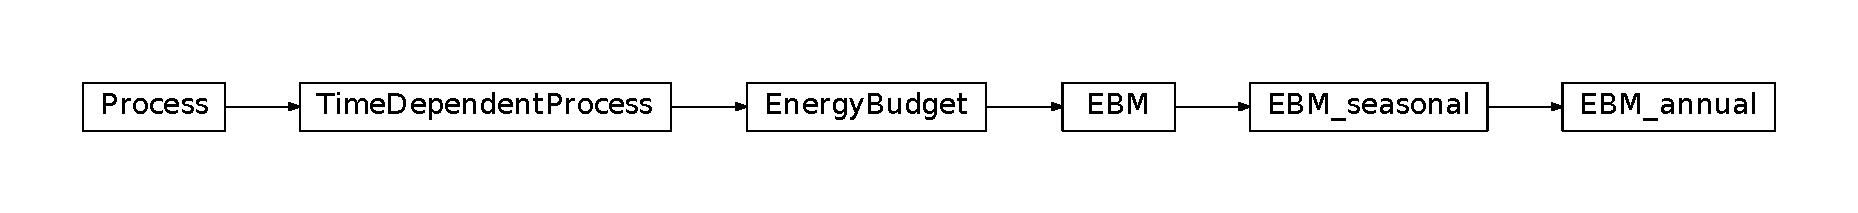
\includegraphics{inheritance-6f4ff43846d3dd82bca0c822ba5c6598e2c24b73.pdf}
\phantomsection\label{api/climlab.model:module-climlab.model.ebm}\index{climlab.model.ebm (module)}\index{EBM (class in climlab.model.ebm)}

\begin{fulllineitems}
\phantomsection\label{api/climlab.model:climlab.model.ebm.EBM}\pysiglinewithargsret{\strong{class }\code{climlab.model.ebm.}\bfcode{EBM}}{\emph{num\_lat=90}, \emph{S0=1365.2}, \emph{A=210.0}, \emph{B=2.0}, \emph{D=0.555}, \emph{water\_depth=10.0}, \emph{Tf=-10.0}, \emph{a0=0.3}, \emph{a2=0.078}, \emph{ai=0.62}, \emph{timestep=350632.51200000005}, \emph{T0=12.0}, \emph{T2=-40.0}, \emph{**kwargs}}{}
Bases: {\hyperref[api/climlab.process:climlab.process.energy_budget.EnergyBudget]{\emph{\code{climlab.process.energy\_budget.EnergyBudget}}}} (\autopageref*{api/climlab.process:climlab.process.energy_budget.EnergyBudget})

A parent class for all Energy-Balance-Model classes.

This class sets up a typical EnergyBalance Model with following subprocesses:
\begin{itemize}
\item {} 
Outgoing Longwave Radiation (OLR) parametrization through 
{\hyperref[api/climlab.radiation:climlab.radiation.AplusBT.AplusBT]{\emph{\code{AplusBT}}}} (\autopageref*{api/climlab.radiation:climlab.radiation.AplusBT.AplusBT})

\item {} 
solar insolation paramtrization through 
{\hyperref[api/climlab.radiation:climlab.radiation.insolation.P2Insolation]{\emph{\code{P2Insolation}}}} (\autopageref*{api/climlab.radiation:climlab.radiation.insolation.P2Insolation})

\item {} 
albedo parametrization in dependence of temperature through
{\hyperref[api/climlab.surface:climlab.surface.albedo.StepFunctionAlbedo]{\emph{\code{StepFunctionAlbedo}}}} (\autopageref*{api/climlab.surface:climlab.surface.albedo.StepFunctionAlbedo})

\item {} 
energy diffusion through 
{\hyperref[api/climlab.dynamics:climlab.dynamics.diffusion.MeridionalDiffusion]{\emph{\code{MeridionalDiffusion}}}} (\autopageref*{api/climlab.dynamics:climlab.dynamics.diffusion.MeridionalDiffusion})

\end{itemize}

\textbf{Initialization parameters}

An instance of \code{EBM} is initialized with the following 
arguments \emph{(for detailed information see Object attributes below)}:
\begin{quote}\begin{description}
\item[{Parameters}] \leavevmode\begin{itemize}
\item {} 
\textbf{\texttt{num\_lat}} (\href{http://docs.python.org/2.7/library/functions.html\#int}{\emph{\texttt{int}}}) -- 
number of equally spaced points for the 
latitue grid. Used for domain intialization of
{\hyperref[api/climlab.domain:climlab.domain.domain.zonal_mean_surface]{\emph{\code{zonal\_mean\_surface}}}} (\autopageref*{api/climlab.domain:climlab.domain.domain.zonal_mean_surface})
\begin{itemize}
\item {} 
default value: \code{90}

\end{itemize}


\item {} 
\textbf{\texttt{S0}} (\href{http://docs.python.org/2.7/library/functions.html\#float}{\emph{\texttt{float}}}) -- 
solar constant
\begin{itemize}
\item {} 
unit: \(\frac{\textrm{W}}{\textrm{m}^2}\)

\item {} 
default value: \code{1365.2}

\end{itemize}


\item {} 
\textbf{\texttt{A}} (\href{http://docs.python.org/2.7/library/functions.html\#float}{\emph{\texttt{float}}}) -- 
parameter for linear OLR parametrization
{\hyperref[api/climlab.radiation:climlab.radiation.AplusBT.AplusBT]{\emph{\code{AplusBT}}}} (\autopageref*{api/climlab.radiation:climlab.radiation.AplusBT.AplusBT})
\begin{itemize}
\item {} 
unit: \(\frac{\textrm{W}}{\textrm{m}^2}\)

\item {} 
default value: \code{210.0}

\end{itemize}


\item {} 
\textbf{\texttt{B}} (\href{http://docs.python.org/2.7/library/functions.html\#float}{\emph{\texttt{float}}}) -- 
parameter for linear OLR parametrization
{\hyperref[api/climlab.radiation:climlab.radiation.AplusBT.AplusBT]{\emph{\code{AplusBT}}}} (\autopageref*{api/climlab.radiation:climlab.radiation.AplusBT.AplusBT})
\begin{itemize}
\item {} 
unit: \(\frac{\textrm{W}}{\textrm{m}^2 \ ^{\circ} \textrm{C}}\)

\item {} 
default value: \code{2.0}

\end{itemize}


\item {} 
\textbf{\texttt{D}} (\href{http://docs.python.org/2.7/library/functions.html\#float}{\emph{\texttt{float}}}) -- 
diffusion parameter for Meridional Energy Diffusion
{\hyperref[api/climlab.dynamics:climlab.dynamics.diffusion.MeridionalDiffusion]{\emph{\code{MeridionalDiffusion}}}} (\autopageref*{api/climlab.dynamics:climlab.dynamics.diffusion.MeridionalDiffusion})
\begin{itemize}
\item {} 
unit: \(\frac{\textrm{W}}{\textrm{m}^2 \ ^{\circ} \textrm{C}}\)

\item {} 
default value: \code{0.555}

\end{itemize}


\item {} 
\textbf{\texttt{water\_depth}} (\href{http://docs.python.org/2.7/library/functions.html\#float}{\emph{\texttt{float}}}) -- 
depth of {\hyperref[api/climlab.domain:climlab.domain.domain.zonal_mean_surface]{\emph{\code{zonal\_mean\_surface}}}} (\autopageref*{api/climlab.domain:climlab.domain.domain.zonal_mean_surface})
domain, which the heat capacity is dependent on
\begin{itemize}
\item {} 
unit: meters

\item {} 
default value: \code{10.0}

\end{itemize}


\item {} 
\textbf{\texttt{Tf}} (\href{http://docs.python.org/2.7/library/functions.html\#float}{\emph{\texttt{float}}}) -- 
freezing temperature
\begin{itemize}
\item {} 
unit: \(^{\circ} \textrm{C}\)

\item {} 
default value: \code{-10.0}

\end{itemize}


\item {} 
\textbf{\texttt{a0}} (\href{http://docs.python.org/2.7/library/functions.html\#float}{\emph{\texttt{float}}}) -- 
base value for planetary albedo parametrization
{\hyperref[api/climlab.surface:climlab.surface.albedo.StepFunctionAlbedo]{\emph{\code{StepFunctionAlbedo}}}} (\autopageref*{api/climlab.surface:climlab.surface.albedo.StepFunctionAlbedo})
\begin{itemize}
\item {} 
unit: dimensionless

\item {} 
default value: \code{0.3}

\end{itemize}


\item {} 
\textbf{\texttt{a2}} (\href{http://docs.python.org/2.7/library/functions.html\#float}{\emph{\texttt{float}}}) -- 
parabolic value for planetary  albedo parametrization
{\hyperref[api/climlab.surface:climlab.surface.albedo.StepFunctionAlbedo]{\emph{\code{StepFunctionAlbedo}}}} (\autopageref*{api/climlab.surface:climlab.surface.albedo.StepFunctionAlbedo})
\begin{itemize}
\item {} 
unit: dimensionless

\item {} 
default value: \code{0.078}

\end{itemize}


\item {} 
\textbf{\texttt{ai}} (\href{http://docs.python.org/2.7/library/functions.html\#float}{\emph{\texttt{float}}}) -- 
value for ice albedo paramerization in
{\hyperref[api/climlab.surface:climlab.surface.albedo.StepFunctionAlbedo]{\emph{\code{StepFunctionAlbedo}}}} (\autopageref*{api/climlab.surface:climlab.surface.albedo.StepFunctionAlbedo})
\begin{itemize}
\item {} 
unit: dimensionless

\item {} 
default value: \code{0.62}

\end{itemize}


\item {} 
\textbf{\texttt{timestep}} (\href{http://docs.python.org/2.7/library/functions.html\#float}{\emph{\texttt{float}}}) -- 
specifies the EBM's timestep
\begin{itemize}
\item {} 
unit: seconds

\item {} 
default value: (365.2422 * 24 * 60 * 60 ) / 90

-\textgreater{} (90 timesteps per year)

\end{itemize}


\item {} 
\textbf{\texttt{T0}} (\href{http://docs.python.org/2.7/library/functions.html\#float}{\emph{\texttt{float}}}) -- 
base value for initial temperature
\begin{itemize}
\item {} 
unit \(^{\circ} \textrm{C}\)

\item {} 
default value: \code{12}

\end{itemize}


\item {} 
\textbf{\texttt{T2}} (\href{http://docs.python.org/2.7/library/functions.html\#float}{\emph{\texttt{float}}}) -- 
factor for 2nd Legendre polynomial 
{\hyperref[api/climlab.utils:climlab.utils.legendre.P2]{\emph{\code{P2}}}} (\autopageref*{api/climlab.utils:climlab.utils.legendre.P2}) 
to calculate initial temperature
\begin{itemize}
\item {} 
unit: dimensionless

\item {} 
default value: \code{40}

\end{itemize}


\end{itemize}

\end{description}\end{quote}

\textbf{Object attributes}

Additional to the parent class {\hyperref[api/climlab.process:climlab.process.energy_budget.EnergyBudget]{\emph{\code{EnergyBudget}}}} (\autopageref*{api/climlab.process:climlab.process.energy_budget.EnergyBudget})
following object attributes are generated and updated during initialization:
\begin{quote}\begin{description}
\item[{Variables}] \leavevmode\begin{itemize}
\item {} 
\textbf{\texttt{param}} (\href{http://docs.python.org/2.7/library/stdtypes.html\#dict}{\emph{\texttt{dict}}}) -- The parameter dictionary is updated with a couple 
of the initatilzation input arguments, namely
\code{'S0'}, \code{'A'}, \code{'B'}, \code{'D'}, \code{'Tf'}, 
\code{'water\_depth'}, \code{'a0'}, \code{'a2'} and \code{'ai'}.

\item {} 
\textbf{\texttt{domains}} (\href{http://docs.python.org/2.7/library/stdtypes.html\#dict}{\emph{\texttt{dict}}}) -- If the object's \code{domains} and the \code{state} 
dictionaries are empty during initialization 
a domain \code{sfc} is created through 
{\hyperref[api/climlab.domain:climlab.domain.domain.zonal_mean_surface]{\emph{\code{zonal\_mean\_surface()}}}} (\autopageref*{api/climlab.domain:climlab.domain.domain.zonal_mean_surface}).
In the meantime the object's \code{domains} and 
\code{state} dictionaries are updated.

\item {} 
\href{http://docs.python.org/2.7/library/subprocess.html\#module-subprocess}{\textbf{\texttt{subprocess}}} (\href{http://docs.python.org/2.7/library/stdtypes.html\#dict}{\emph{\texttt{dict}}}) -- Several subprocesses are created (see above) 
through calling 
{\hyperref[api/climlab.process:climlab.process.process.Process.add_subprocess]{\emph{\code{add\_subprocess()}}}} (\autopageref*{api/climlab.process:climlab.process.process.Process.add_subprocess})
and therefore the subprocess dictionary is updated.

\item {} 
\textbf{\texttt{topdown}} (\href{http://docs.python.org/2.7/library/functions.html\#bool}{\emph{\texttt{bool}}}) -- is set to \code{False} to call subprocess compute 
methods first.
See also 
{\hyperref[api/climlab.process:climlab.process.time_dependent_process.TimeDependentProcess]{\emph{\code{TimeDependentProcess}}}} (\autopageref*{api/climlab.process:climlab.process.time_dependent_process.TimeDependentProcess}).

\item {} 
\textbf{\texttt{diagnostics}} (\href{http://docs.python.org/2.7/library/stdtypes.html\#dict}{\emph{\texttt{dict}}}) -- is initialized with keys: \code{'OLR'}, \code{'ASR'},
\code{'net\_radiation'}, \code{'albedo'} and \code{'icelat'}
through 
{\hyperref[api/climlab.process:climlab.process.process.Process.init_diagnostic]{\emph{\code{init\_diagnostic()}}}} (\autopageref*{api/climlab.process:climlab.process.process.Process.init_diagnostic}).

\end{itemize}

\item[{Example}] \leavevmode
Creation and integration of the preconfigured Energy Balance Model:

\begin{Verbatim}[commandchars=\\\{\}]
\PYG{g+gp}{\PYGZgt{}\PYGZgt{}\PYGZgt{} }\PYG{k+kn}{import} \PYG{n+nn}{climlab}
\PYG{g+gp}{\PYGZgt{}\PYGZgt{}\PYGZgt{} }\PYG{n}{model} \PYG{o}{=} \PYG{n}{climlab}\PYG{o}{.}\PYG{n}{EBM}\PYG{p}{(}\PYG{p}{)}

\PYG{g+gp}{\PYGZgt{}\PYGZgt{}\PYGZgt{} }\PYG{n}{model}\PYG{o}{.}\PYG{n}{integrate\PYGZus{}years}\PYG{p}{(}\PYG{l+m+mf}{2.}\PYG{p}{)}
\PYG{g+go}{Integrating for 180 steps, 730.4844 days, or 2.0 years.}
\PYG{g+go}{Total elapsed time is 2.0 years.}
\end{Verbatim}

For more information how to use the EBM class, see the {\hyperref[tutorial:tutorial]{\emph{Tutorials}}} (\autopageref*{tutorial:tutorial}) 
chapter.

\end{description}\end{quote}
\index{diffusive\_heat\_transport() (climlab.model.ebm.EBM method)}

\begin{fulllineitems}
\phantomsection\label{api/climlab.model:climlab.model.ebm.EBM.diffusive_heat_transport}\pysiglinewithargsret{\bfcode{diffusive\_heat\_transport}}{}{}
Compute instantaneous diffusive heat transport in unit \(\textrm{PW}\)
on the staggered grid (bounds) through calculating:
\begin{gather}
\begin{split}H(\varphi) = - 2 \pi R^2 cos(\varphi) D \frac{dT}{d\varphi}
            \approx - 2 \pi R^2 cos(\varphi) D \frac{\Delta T}{\Delta \varphi}\end{split}\notag
\end{gather}\begin{quote}\begin{description}
\item[{Return type}] \leavevmode
array of size \code{np.size(self.lat\_bounds)}

\end{description}\end{quote}

\end{fulllineitems}

\index{global\_mean\_temperature() (climlab.model.ebm.EBM method)}

\begin{fulllineitems}
\phantomsection\label{api/climlab.model:climlab.model.ebm.EBM.global_mean_temperature}\pysiglinewithargsret{\bfcode{global\_mean\_temperature}}{}{}
Convenience method to compute global mean surface temperature.

Calls {\hyperref[api/climlab.domain:climlab.domain.field.global_mean]{\emph{\code{global\_mean()}}}} (\autopageref*{api/climlab.domain:climlab.domain.field.global_mean}) method which
for the object attriute \code{Ts} which calculates the latitude weighted
global mean of a field.
\begin{quote}\begin{description}
\item[{Example}] \leavevmode
Calculating the global mean temperature of initial EBM temperature:

\begin{Verbatim}[commandchars=\\\{\}]
\PYG{g+gp}{\PYGZgt{}\PYGZgt{}\PYGZgt{} }\PYG{k+kn}{import} \PYG{n+nn}{climlab}
\PYG{g+gp}{\PYGZgt{}\PYGZgt{}\PYGZgt{} }\PYG{n}{model} \PYG{o}{=} \PYG{n}{climlab}\PYG{o}{.}\PYG{n}{EBM}\PYG{p}{(}\PYG{n}{T0}\PYG{o}{=}\PYG{l+m+mf}{14.}\PYG{p}{,} \PYG{n}{T2}\PYG{o}{=}\PYG{o}{\PYGZhy{}}\PYG{l+m+mi}{25}\PYG{p}{)}

\PYG{g+gp}{\PYGZgt{}\PYGZgt{}\PYGZgt{} }\PYG{n}{model}\PYG{o}{.}\PYG{n}{global\PYGZus{}mean\PYGZus{}temperature}\PYG{p}{(}\PYG{p}{)}
\PYG{g+go}{Field(13.99873037400856)}
\end{Verbatim}

\end{description}\end{quote}

\end{fulllineitems}

\index{heat\_transport() (climlab.model.ebm.EBM method)}

\begin{fulllineitems}
\phantomsection\label{api/climlab.model:climlab.model.ebm.EBM.heat_transport}\pysiglinewithargsret{\bfcode{heat\_transport}}{}{}
Returns instantaneous heat transport in unit \(\textrm{PW}\)
on the staggered grid (bounds) through calling
{\hyperref[api/climlab.model:climlab.model.ebm.EBM.diffusive_heat_transport]{\emph{\code{diffusive\_heat\_transport()}}}} (\autopageref*{api/climlab.model:climlab.model.ebm.EBM.diffusive_heat_transport}).
\begin{quote}\begin{description}
\item[{Example}] \leavevmode
\begin{Verbatim}[commandchars=\\\{\}]
\PYG{k+kn}{import} \PYG{n+nn}{climlab}
\PYG{k+kn}{import} \PYG{n+nn}{matplotlib.pyplot} \PYG{k+kn}{as} \PYG{n+nn}{plt}

\PYG{c+c1}{\PYGZsh{} creating \PYGZam{} integrating model}
\PYG{n}{model} \PYG{o}{=} \PYG{n}{climlab}\PYG{o}{.}\PYG{n}{EBM}\PYG{p}{(}\PYG{p}{)}
\PYG{n}{model}\PYG{o}{.}\PYG{n}{step\PYGZus{}forward}\PYG{p}{(}\PYG{p}{)}

\PYG{c+c1}{\PYGZsh{} plot}
\PYG{n}{fig} \PYG{o}{=} \PYG{n}{plt}\PYG{o}{.}\PYG{n}{figure}\PYG{p}{(} \PYG{n}{figsize}\PYG{o}{=}\PYG{p}{(}\PYG{l+m+mi}{6}\PYG{p}{,}\PYG{l+m+mi}{4}\PYG{p}{)}\PYG{p}{)}
\PYG{n}{ax} \PYG{o}{=} \PYG{n}{fig}\PYG{o}{.}\PYG{n}{add\PYGZus{}subplot}\PYG{p}{(}\PYG{l+m+mi}{111}\PYG{p}{)}

\PYG{n}{bounds} \PYG{o}{=} \PYG{n}{model}\PYG{o}{.}\PYG{n}{domains}\PYG{p}{[}\PYG{l+s+s1}{\PYGZsq{}}\PYG{l+s+s1}{Ts}\PYG{l+s+s1}{\PYGZsq{}}\PYG{p}{]}\PYG{o}{.}\PYG{n}{axes}\PYG{p}{[}\PYG{l+s+s1}{\PYGZsq{}}\PYG{l+s+s1}{lat}\PYG{l+s+s1}{\PYGZsq{}}\PYG{p}{]}\PYG{o}{.}\PYG{n}{bounds}
\PYG{n}{ax}\PYG{o}{.}\PYG{n}{plot}\PYG{p}{(}\PYG{n}{bounds}\PYG{p}{,} \PYG{n}{model}\PYG{o}{.}\PYG{n}{heat\PYGZus{}transport}\PYG{p}{(}\PYG{p}{)}\PYG{p}{)}

\PYG{n}{ax}\PYG{o}{.}\PYG{n}{set\PYGZus{}title}\PYG{p}{(}\PYG{l+s+s1}{\PYGZsq{}}\PYG{l+s+s1}{heat transport}\PYG{l+s+s1}{\PYGZsq{}}\PYG{p}{)}
\PYG{n}{ax}\PYG{o}{.}\PYG{n}{set\PYGZus{}xlabel}\PYG{p}{(}\PYG{l+s+s1}{\PYGZsq{}}\PYG{l+s+s1}{latitude}\PYG{l+s+s1}{\PYGZsq{}}\PYG{p}{)}
\PYG{n}{ax}\PYG{o}{.}\PYG{n}{set\PYGZus{}xticks}\PYG{p}{(}\PYG{p}{[}\PYG{o}{\PYGZhy{}}\PYG{l+m+mi}{90}\PYG{p}{,}\PYG{o}{\PYGZhy{}}\PYG{l+m+mi}{60}\PYG{p}{,}\PYG{o}{\PYGZhy{}}\PYG{l+m+mi}{30}\PYG{p}{,}\PYG{l+m+mi}{0}\PYG{p}{,}\PYG{l+m+mi}{30}\PYG{p}{,}\PYG{l+m+mi}{60}\PYG{p}{,}\PYG{l+m+mi}{90}\PYG{p}{]}\PYG{p}{)}
\PYG{n}{ax}\PYG{o}{.}\PYG{n}{set\PYGZus{}ylabel}\PYG{p}{(}\PYG{l+s+s1}{\PYGZsq{}}\PYG{l+s+s1}{energy (PW)}\PYG{l+s+s1}{\PYGZsq{}}\PYG{p}{)}
\PYG{n}{plt}\PYG{o}{.}\PYG{n}{axhline}\PYG{p}{(}\PYG{n}{linewidth}\PYG{o}{=}\PYG{l+m+mi}{2}\PYG{p}{,} \PYG{n}{color}\PYG{o}{=}\PYG{l+s+s1}{\PYGZsq{}}\PYG{l+s+s1}{grey}\PYG{l+s+s1}{\PYGZsq{}}\PYG{p}{,} \PYG{n}{linestyle}\PYG{o}{=}\PYG{l+s+s1}{\PYGZsq{}}\PYG{l+s+s1}{dashed}\PYG{l+s+s1}{\PYGZsq{}}\PYG{p}{)}
\PYG{n}{plt}\PYG{o}{.}\PYG{n}{show}\PYG{p}{(}\PYG{p}{)}
\end{Verbatim}

\includegraphics{{example_EBM_heat_transport}.pdf}

\end{description}\end{quote}

\end{fulllineitems}

\index{heat\_transport\_convergence() (climlab.model.ebm.EBM method)}

\begin{fulllineitems}
\phantomsection\label{api/climlab.model:climlab.model.ebm.EBM.heat_transport_convergence}\pysiglinewithargsret{\bfcode{heat\_transport\_convergence}}{}{}
Returns instantaneous convergence of heat transport.
\begin{gather}
\begin{split}h(\varphi) = - \frac{1}{2 \pi R^2 cos(\varphi)} \frac{dH}{d\varphi} 
            \approx - \frac{1}{2 \pi R^2 cos(\varphi)} \frac{\Delta H}{\Delta \varphi} \end{split}\notag
\end{gather}
h is the \emph{dynamical heating rate} in unit \(\textrm{W}/ \textrm{m}^2\)
which is the convergence of energy transport into each latitude band,
namely the difference between what's coming in and what's going out.
\begin{quote}\begin{description}
\item[{Example}] \leavevmode
\begin{Verbatim}[commandchars=\\\{\}]
\PYG{k+kn}{import} \PYG{n+nn}{climlab}
\PYG{k+kn}{import} \PYG{n+nn}{matplotlib.pyplot} \PYG{k+kn}{as} \PYG{n+nn}{plt}

\PYG{c+c1}{\PYGZsh{} creating \PYGZam{} integrating model}
\PYG{n}{model} \PYG{o}{=} \PYG{n}{climlab}\PYG{o}{.}\PYG{n}{EBM}\PYG{p}{(}\PYG{p}{)}
\PYG{n}{model}\PYG{o}{.}\PYG{n}{integrate\PYGZus{}converge}\PYG{p}{(}\PYG{p}{)}

\PYG{c+c1}{\PYGZsh{} plot}
\PYG{n}{fig} \PYG{o}{=} \PYG{n}{plt}\PYG{o}{.}\PYG{n}{figure}\PYG{p}{(} \PYG{n}{figsize}\PYG{o}{=}\PYG{p}{(}\PYG{l+m+mi}{6}\PYG{p}{,}\PYG{l+m+mi}{4}\PYG{p}{)}\PYG{p}{)}
\PYG{n}{ax} \PYG{o}{=} \PYG{n}{fig}\PYG{o}{.}\PYG{n}{add\PYGZus{}subplot}\PYG{p}{(}\PYG{l+m+mi}{111}\PYG{p}{)}

\PYG{n}{ax}\PYG{o}{.}\PYG{n}{plot}\PYG{p}{(}\PYG{n}{model}\PYG{o}{.}\PYG{n}{lat}\PYG{p}{,} \PYG{n}{model}\PYG{o}{.}\PYG{n}{heat\PYGZus{}transport\PYGZus{}convergence}\PYG{p}{(}\PYG{p}{)}\PYG{p}{)}

\PYG{n}{ax}\PYG{o}{.}\PYG{n}{set\PYGZus{}title}\PYG{p}{(}\PYG{l+s+s1}{\PYGZsq{}}\PYG{l+s+s1}{heat transport convergence}\PYG{l+s+s1}{\PYGZsq{}}\PYG{p}{)}
\PYG{n}{ax}\PYG{o}{.}\PYG{n}{set\PYGZus{}xlabel}\PYG{p}{(}\PYG{l+s+s1}{\PYGZsq{}}\PYG{l+s+s1}{latitude}\PYG{l+s+s1}{\PYGZsq{}}\PYG{p}{)}
\PYG{n}{ax}\PYG{o}{.}\PYG{n}{set\PYGZus{}xticks}\PYG{p}{(}\PYG{p}{[}\PYG{o}{\PYGZhy{}}\PYG{l+m+mi}{90}\PYG{p}{,}\PYG{o}{\PYGZhy{}}\PYG{l+m+mi}{60}\PYG{p}{,}\PYG{o}{\PYGZhy{}}\PYG{l+m+mi}{30}\PYG{p}{,}\PYG{l+m+mi}{0}\PYG{p}{,}\PYG{l+m+mi}{30}\PYG{p}{,}\PYG{l+m+mi}{60}\PYG{p}{,}\PYG{l+m+mi}{90}\PYG{p}{]}\PYG{p}{)}
\PYG{n}{ax}\PYG{o}{.}\PYG{n}{set\PYGZus{}ylabel}\PYG{p}{(}\PYG{l+s+s1}{\PYGZsq{}}\PYG{l+s+s1}{energy (W/m\PYGZdl{}\PYGZca{}2\PYGZdl{})}\PYG{l+s+s1}{\PYGZsq{}}\PYG{p}{)}
\PYG{n}{plt}\PYG{o}{.}\PYG{n}{axhline}\PYG{p}{(}\PYG{n}{linewidth}\PYG{o}{=}\PYG{l+m+mi}{2}\PYG{p}{,} \PYG{n}{color}\PYG{o}{=}\PYG{l+s+s1}{\PYGZsq{}}\PYG{l+s+s1}{grey}\PYG{l+s+s1}{\PYGZsq{}}\PYG{p}{,} \PYG{n}{linestyle}\PYG{o}{=}\PYG{l+s+s1}{\PYGZsq{}}\PYG{l+s+s1}{dashed}\PYG{l+s+s1}{\PYGZsq{}}\PYG{p}{)}
\PYG{n}{plt}\PYG{o}{.}\PYG{n}{show}\PYG{p}{(}\PYG{p}{)}
\end{Verbatim}

\includegraphics{{example_EBM_heat_transport_convergence}.pdf}

\end{description}\end{quote}

\end{fulllineitems}

\index{inferred\_heat\_transport() (climlab.model.ebm.EBM method)}

\begin{fulllineitems}
\phantomsection\label{api/climlab.model:climlab.model.ebm.EBM.inferred_heat_transport}\pysiglinewithargsret{\bfcode{inferred\_heat\_transport}}{}{}
Calculates the inferred heat transport by integrating the TOA 
energy imbalance from pole to pole.

The method is calculating
\begin{gather}
\begin{split}H(\varphi) = 2 \pi R^2 \int_{-\pi/2}^{\varphi} cos\phi \ R_{TOA} d\phi\end{split}\notag
\end{gather}
where \(R_{TOA}\) is the net radiation at top of atmosphere.
\begin{quote}\begin{description}
\item[{Returns}] \leavevmode
total heat transport on the latitude grid in unit \(\textrm{PW}\)

\item[{Return type}] \leavevmode
array of size \code{np.size(self.lat\_lat)}

\item[{Example}] \leavevmode
\begin{Verbatim}[commandchars=\\\{\}]
\PYG{k+kn}{import} \PYG{n+nn}{climlab}
\PYG{k+kn}{import} \PYG{n+nn}{matplotlib.pyplot} \PYG{k+kn}{as} \PYG{n+nn}{plt}

\PYG{c+c1}{\PYGZsh{} creating \PYGZam{} integrating model}
\PYG{n}{model} \PYG{o}{=} \PYG{n}{climlab}\PYG{o}{.}\PYG{n}{EBM}\PYG{p}{(}\PYG{p}{)}
\PYG{n}{model}\PYG{o}{.}\PYG{n}{step\PYGZus{}forward}\PYG{p}{(}\PYG{p}{)}

\PYG{c+c1}{\PYGZsh{} plot}
\PYG{n}{fig} \PYG{o}{=} \PYG{n}{plt}\PYG{o}{.}\PYG{n}{figure}\PYG{p}{(} \PYG{n}{figsize}\PYG{o}{=}\PYG{p}{(}\PYG{l+m+mi}{6}\PYG{p}{,}\PYG{l+m+mi}{4}\PYG{p}{)}\PYG{p}{)}
\PYG{n}{ax} \PYG{o}{=} \PYG{n}{fig}\PYG{o}{.}\PYG{n}{add\PYGZus{}subplot}\PYG{p}{(}\PYG{l+m+mi}{111}\PYG{p}{)}

\PYG{n}{ax}\PYG{o}{.}\PYG{n}{plot}\PYG{p}{(}\PYG{n}{model}\PYG{o}{.}\PYG{n}{lat}\PYG{p}{,} \PYG{n}{model}\PYG{o}{.}\PYG{n}{inferred\PYGZus{}heat\PYGZus{}transport}\PYG{p}{(}\PYG{p}{)}\PYG{p}{)}

\PYG{n}{ax}\PYG{o}{.}\PYG{n}{set\PYGZus{}title}\PYG{p}{(}\PYG{l+s+s1}{\PYGZsq{}}\PYG{l+s+s1}{inferred heat transport}\PYG{l+s+s1}{\PYGZsq{}}\PYG{p}{)}
\PYG{n}{ax}\PYG{o}{.}\PYG{n}{set\PYGZus{}xlabel}\PYG{p}{(}\PYG{l+s+s1}{\PYGZsq{}}\PYG{l+s+s1}{latitude}\PYG{l+s+s1}{\PYGZsq{}}\PYG{p}{)}
\PYG{n}{ax}\PYG{o}{.}\PYG{n}{set\PYGZus{}xticks}\PYG{p}{(}\PYG{p}{[}\PYG{o}{\PYGZhy{}}\PYG{l+m+mi}{90}\PYG{p}{,}\PYG{o}{\PYGZhy{}}\PYG{l+m+mi}{60}\PYG{p}{,}\PYG{o}{\PYGZhy{}}\PYG{l+m+mi}{30}\PYG{p}{,}\PYG{l+m+mi}{0}\PYG{p}{,}\PYG{l+m+mi}{30}\PYG{p}{,}\PYG{l+m+mi}{60}\PYG{p}{,}\PYG{l+m+mi}{90}\PYG{p}{]}\PYG{p}{)}
\PYG{n}{ax}\PYG{o}{.}\PYG{n}{set\PYGZus{}ylabel}\PYG{p}{(}\PYG{l+s+s1}{\PYGZsq{}}\PYG{l+s+s1}{energy (PW)}\PYG{l+s+s1}{\PYGZsq{}}\PYG{p}{)}
\PYG{n}{plt}\PYG{o}{.}\PYG{n}{axhline}\PYG{p}{(}\PYG{n}{linewidth}\PYG{o}{=}\PYG{l+m+mi}{2}\PYG{p}{,} \PYG{n}{color}\PYG{o}{=}\PYG{l+s+s1}{\PYGZsq{}}\PYG{l+s+s1}{grey}\PYG{l+s+s1}{\PYGZsq{}}\PYG{p}{,} \PYG{n}{linestyle}\PYG{o}{=}\PYG{l+s+s1}{\PYGZsq{}}\PYG{l+s+s1}{dashed}\PYG{l+s+s1}{\PYGZsq{}}\PYG{p}{)}
\PYG{n}{plt}\PYG{o}{.}\PYG{n}{show}\PYG{p}{(}\PYG{p}{)}
\end{Verbatim}

\includegraphics{{example_EBM_inferred_heat_transport}.pdf}

\end{description}\end{quote}

\end{fulllineitems}


\end{fulllineitems}

\index{EBM\_annual (class in climlab.model.ebm)}

\begin{fulllineitems}
\phantomsection\label{api/climlab.model:climlab.model.ebm.EBM_annual}\pysiglinewithargsret{\strong{class }\code{climlab.model.ebm.}\bfcode{EBM\_annual}}{\emph{**kwargs}}{}
Bases: {\hyperref[api/climlab.model:climlab.model.ebm.EBM_seasonal]{\emph{\code{climlab.model.ebm.EBM\_seasonal}}}} (\autopageref*{api/climlab.model:climlab.model.ebm.EBM_seasonal})

A class that implements Energy Balance Models with annual mean insolation.

The annual solar distribution is calculated through averaging the 
{\hyperref[api/climlab.radiation:climlab.radiation.insolation.DailyInsolation]{\emph{\code{DailyInsolation}}}} (\autopageref*{api/climlab.radiation:climlab.radiation.insolation.DailyInsolation}) over time 
which has been used in used in the parent class
{\hyperref[api/climlab.model:climlab.model.ebm.EBM_seasonal]{\emph{\code{EBM\_seasonal}}}} (\autopageref*{api/climlab.model:climlab.model.ebm.EBM_seasonal}). That is done by the subprocess
{\hyperref[api/climlab.radiation:climlab.radiation.insolation.AnnualMeanInsolation]{\emph{\code{AnnualMeanInsolation}}}} (\autopageref*{api/climlab.radiation:climlab.radiation.insolation.AnnualMeanInsolation}) which is
more realistic than the {\hyperref[api/climlab.radiation:climlab.radiation.insolation.P2Insolation]{\emph{\code{P2Insolation}}}} (\autopageref*{api/climlab.radiation:climlab.radiation.insolation.P2Insolation})
module used in the classical {\hyperref[api/climlab.model:climlab.model.ebm.EBM]{\emph{\code{EBM}}}} (\autopageref*{api/climlab.model:climlab.model.ebm.EBM}) class.

According to the parent class {\hyperref[api/climlab.model:climlab.model.ebm.EBM_seasonal]{\emph{\code{EBM\_seasonal}}}} (\autopageref*{api/climlab.model:climlab.model.ebm.EBM_seasonal})
the model will not have an ice-albedo feedback, if albedo ice parameter
\code{'ai'} is not given. For details see there.

\textbf{Object attributes}

Following object attributes are updated during initialization:
\begin{quote}\begin{description}
\item[{Variables}] \leavevmode
\href{http://docs.python.org/2.7/library/subprocess.html\#module-subprocess}{\textbf{\texttt{subprocess}}} (\href{http://docs.python.org/2.7/library/stdtypes.html\#dict}{\emph{\texttt{dict}}}) -- suprocess \code{'insolation'} is overwritten by
{\hyperref[api/climlab.radiation:climlab.radiation.insolation.AnnualMeanInsolation]{\emph{\code{AnnualMeanInsolation}}}} (\autopageref*{api/climlab.radiation:climlab.radiation.insolation.AnnualMeanInsolation})

\item[{Example}] \leavevmode
The {\hyperref[api/climlab.model:climlab.model.ebm.EBM_annual]{\emph{\code{EBM\_annual}}}} (\autopageref*{api/climlab.model:climlab.model.ebm.EBM_annual}) class uses a different 
insolation subprocess than the {\hyperref[api/climlab.model:climlab.model.ebm.EBM]{\emph{\code{EBM}}}} (\autopageref*{api/climlab.model:climlab.model.ebm.EBM}) class:

\begin{Verbatim}[commandchars=\\\{\}]
\PYG{g+gp}{\PYGZgt{}\PYGZgt{}\PYGZgt{} }\PYG{k+kn}{import} \PYG{n+nn}{climlab}
\PYG{g+gp}{\PYGZgt{}\PYGZgt{}\PYGZgt{} }\PYG{n}{model\PYGZus{}annual} \PYG{o}{=} \PYG{n}{climlab}\PYG{o}{.}\PYG{n}{EBM\PYGZus{}annual}\PYG{p}{(}\PYG{p}{)}

\PYG{g+gp}{\PYGZgt{}\PYGZgt{}\PYGZgt{} }\PYG{k}{print} \PYG{n}{model\PYGZus{}annual}
\end{Verbatim}

\begin{Verbatim}[commandchars=\\\{\}]
 climlab Process of type \PYGZlt{}class \PYGZsq{}climlab.model.ebm.EBM\PYGZus{}annual\PYGZsq{}\PYGZgt{}. 
 State variables and domain shapes: 
   Ts: (90, 1) 
 The subprocess tree: 
 top: \PYGZlt{}class \PYGZsq{}climlab.model.ebm.EBM\PYGZus{}annual\PYGZsq{}\PYGZgt{}
    diffusion: \PYGZlt{}class \PYGZsq{}climlab.dynamics.diffusion.MeridionalDiffusion\PYGZsq{}\PYGZgt{}
    LW: \PYGZlt{}class \PYGZsq{}climlab.radiation.AplusBT.AplusBT\PYGZsq{}\PYGZgt{}
    albedo: \PYGZlt{}class \PYGZsq{}climlab.surface.albedo.P2Albedo\PYGZsq{}\PYGZgt{}
    insolation: \PYGZlt{}class \PYGZsq{}climlab.radiation.insolation.AnnualMeanInsolation\PYGZsq{}\PYGZgt{}
\end{Verbatim}

\end{description}\end{quote}

\end{fulllineitems}

\index{EBM\_seasonal (class in climlab.model.ebm)}

\begin{fulllineitems}
\phantomsection\label{api/climlab.model:climlab.model.ebm.EBM_seasonal}\pysiglinewithargsret{\strong{class }\code{climlab.model.ebm.}\bfcode{EBM\_seasonal}}{\emph{a0=0.33}, \emph{a2=0.25}, \emph{ai=None}, \emph{**kwargs}}{}
Bases: {\hyperref[api/climlab.model:climlab.model.ebm.EBM]{\emph{\code{climlab.model.ebm.EBM}}}} (\autopageref*{api/climlab.model:climlab.model.ebm.EBM})

A class that implements Energy Balance Models with realistic 
daily insolation.

This class is inherited from the general {\hyperref[api/climlab.model:climlab.model.ebm.EBM]{\emph{\code{EBM}}}} (\autopageref*{api/climlab.model:climlab.model.ebm.EBM})
class and uses the insolation subprocess 
{\hyperref[api/climlab.radiation:climlab.radiation.insolation.DailyInsolation]{\emph{\code{DailyInsolation}}}} (\autopageref*{api/climlab.radiation:climlab.radiation.insolation.DailyInsolation}) instead of 
{\hyperref[api/climlab.radiation:climlab.radiation.insolation.P2Insolation]{\emph{\code{P2Insolation}}}} (\autopageref*{api/climlab.radiation:climlab.radiation.insolation.P2Insolation}) to compute a
realisitc distribution of solar radiation on a daily basis.

If argument for ice albedo \code{'ai'} is not given, the model will not 
have an albedo feedback.

An instance of \code{EBM\_seasonal} is initialized with the following 
arguments:
\begin{quote}\begin{description}
\item[{Parameters}] \leavevmode\begin{itemize}
\item {} 
\textbf{\texttt{a0}} (\href{http://docs.python.org/2.7/library/functions.html\#float}{\emph{\texttt{float}}}) -- base value for planetary albedo parametrization
{\hyperref[api/climlab.surface:climlab.surface.albedo.StepFunctionAlbedo]{\emph{\code{StepFunctionAlbedo}}}} (\autopageref*{api/climlab.surface:climlab.surface.albedo.StepFunctionAlbedo})
{[}default: 0.33{]}

\item {} 
\textbf{\texttt{a2}} (\href{http://docs.python.org/2.7/library/functions.html\#float}{\emph{\texttt{float}}}) -- parabolic value for planetary  albedo parametrization
{\hyperref[api/climlab.surface:climlab.surface.albedo.StepFunctionAlbedo]{\emph{\code{StepFunctionAlbedo}}}} (\autopageref*{api/climlab.surface:climlab.surface.albedo.StepFunctionAlbedo})
{[}default: 0.25{]}

\item {} 
\textbf{\texttt{ai}} (\href{http://docs.python.org/2.7/library/functions.html\#float}{\emph{\texttt{float}}}) -- value for ice albedo paramerization in
{\hyperref[api/climlab.surface:climlab.surface.albedo.StepFunctionAlbedo]{\emph{\code{StepFunctionAlbedo}}}} (\autopageref*{api/climlab.surface:climlab.surface.albedo.StepFunctionAlbedo})
(optional)

\end{itemize}

\end{description}\end{quote}

\textbf{Object attributes}

Following object attributes are updated during initialization:
\begin{quote}\begin{description}
\item[{Variables}] \leavevmode\begin{itemize}
\item {} 
\textbf{\texttt{param}} (\href{http://docs.python.org/2.7/library/stdtypes.html\#dict}{\emph{\texttt{dict}}}) -- The parameter dictionary is updated with 
\code{'a0'} and \code{'a2'}.

\item {} 
\href{http://docs.python.org/2.7/library/subprocess.html\#module-subprocess}{\textbf{\texttt{subprocess}}} (\href{http://docs.python.org/2.7/library/stdtypes.html\#dict}{\emph{\texttt{dict}}}) -- suprocess \code{'insolation'} is overwritten by
{\hyperref[api/climlab.radiation:climlab.radiation.insolation.DailyInsolation]{\emph{\code{DailyInsolation}}}} (\autopageref*{api/climlab.radiation:climlab.radiation.insolation.DailyInsolation}).

\end{itemize}

\end{description}\end{quote}

\emph{if} \code{'ai'} \emph{is not given}:
\begin{quote}\begin{description}
\item[{Variables}] \leavevmode\begin{itemize}
\item {} 
\textbf{\texttt{param}} (\href{http://docs.python.org/2.7/library/stdtypes.html\#dict}{\emph{\texttt{dict}}}) -- \code{'ai'} and \code{'Tf'} are removed from the 
parameter dictionary (initialized by parent class
{\hyperref[api/climlab.model:climlab.model.ebm.EBM]{\emph{\code{EBM}}}} (\autopageref*{api/climlab.model:climlab.model.ebm.EBM}))

\item {} 
\href{http://docs.python.org/2.7/library/subprocess.html\#module-subprocess}{\textbf{\texttt{subprocess}}} (\href{http://docs.python.org/2.7/library/stdtypes.html\#dict}{\emph{\texttt{dict}}}) -- suprocess \code{'albedo'} is overwritten by
{\hyperref[api/climlab.surface:climlab.surface.albedo.P2Albedo]{\emph{\code{P2Albedo}}}} (\autopageref*{api/climlab.surface:climlab.surface.albedo.P2Albedo}).

\end{itemize}

\end{description}\end{quote}

\emph{if} \code{'ai'} \emph{is given}:
\begin{quote}\begin{description}
\item[{Variables}] \leavevmode\begin{itemize}
\item {} 
\textbf{\texttt{param}} (\href{http://docs.python.org/2.7/library/stdtypes.html\#dict}{\emph{\texttt{dict}}}) -- The parameter dictionary is updated with
\code{'ai'}.

\item {} 
\href{http://docs.python.org/2.7/library/subprocess.html\#module-subprocess}{\textbf{\texttt{subprocess}}} (\href{http://docs.python.org/2.7/library/stdtypes.html\#dict}{\emph{\texttt{dict}}}) -- suprocess \code{'albedo'} is overwritten by
{\hyperref[api/climlab.surface:climlab.surface.albedo.StepFunctionAlbedo]{\emph{\code{StepFunctionAlbedo}}}} (\autopageref*{api/climlab.surface:climlab.surface.albedo.StepFunctionAlbedo}) 
(which basically has been there before but now is 
updated with the new albedo parameter values).

\end{itemize}

\item[{Example}] \leavevmode
The annual distribution of solar insolation:

\begin{Verbatim}[commandchars=\\\{\}]
\PYG{k+kn}{import} \PYG{n+nn}{climlab}
\PYG{k+kn}{from} \PYG{n+nn}{climlab.utils} \PYG{k+kn}{import} \PYG{n}{constants} \PYG{k}{as} \PYG{n}{const}
\PYG{k+kn}{import} \PYG{n+nn}{numpy} \PYG{k+kn}{as} \PYG{n+nn}{np}
\PYG{k+kn}{import} \PYG{n+nn}{matplotlib.pyplot} \PYG{k+kn}{as} \PYG{n+nn}{plt}

\PYG{c+c1}{\PYGZsh{} creating model}
\PYG{n}{model} \PYG{o}{=} \PYG{n}{climlab}\PYG{o}{.}\PYG{n}{EBM\PYGZus{}seasonal}\PYG{p}{(}\PYG{p}{)}
\PYG{n}{model}\PYG{o}{.}\PYG{n}{step\PYGZus{}forward}\PYG{p}{(}\PYG{p}{)}

\PYG{n}{solar} \PYG{o}{=} \PYG{n}{model}\PYG{o}{.}\PYG{n}{subprocess}\PYG{p}{[}\PYG{l+s+s1}{\PYGZsq{}}\PYG{l+s+s1}{insolation}\PYG{l+s+s1}{\PYGZsq{}}\PYG{p}{]}\PYG{o}{.}\PYG{n}{insolation}

\PYG{c+c1}{\PYGZsh{} plot}
\PYG{n}{fig} \PYG{o}{=} \PYG{n}{plt}\PYG{o}{.}\PYG{n}{figure}\PYG{p}{(} \PYG{n}{figsize}\PYG{o}{=}\PYG{p}{(}\PYG{l+m+mi}{6}\PYG{p}{,}\PYG{l+m+mi}{4}\PYG{p}{)}\PYG{p}{)}
\PYG{n}{ax} \PYG{o}{=} \PYG{n}{fig}\PYG{o}{.}\PYG{n}{add\PYGZus{}subplot}\PYG{p}{(}\PYG{l+m+mi}{111}\PYG{p}{)}

\PYG{n}{season\PYGZus{}days} \PYG{o}{=} \PYG{n}{const}\PYG{o}{.}\PYG{n}{days\PYGZus{}per\PYGZus{}year}\PYG{o}{/}\PYG{l+m+mi}{4}

\PYG{k}{for} \PYG{n}{season} \PYG{o+ow}{in} \PYG{p}{[}\PYG{l+s+s1}{\PYGZsq{}}\PYG{l+s+s1}{winter}\PYG{l+s+s1}{\PYGZsq{}}\PYG{p}{,}\PYG{l+s+s1}{\PYGZsq{}}\PYG{l+s+s1}{spring}\PYG{l+s+s1}{\PYGZsq{}}\PYG{p}{,}\PYG{l+s+s1}{\PYGZsq{}}\PYG{l+s+s1}{summer}\PYG{l+s+s1}{\PYGZsq{}}\PYG{p}{,}\PYG{l+s+s1}{\PYGZsq{}}\PYG{l+s+s1}{autumn}\PYG{l+s+s1}{\PYGZsq{}}\PYG{p}{]}\PYG{p}{:}
    \PYG{n}{ax}\PYG{o}{.}\PYG{n}{plot}\PYG{p}{(}\PYG{n}{model}\PYG{o}{.}\PYG{n}{lat}\PYG{p}{,} \PYG{n}{solar}\PYG{p}{,} \PYG{n}{label}\PYG{o}{=}\PYG{n}{season}\PYG{p}{)}
    \PYG{n}{model}\PYG{o}{.}\PYG{n}{integrate\PYGZus{}days}\PYG{p}{(}\PYG{n}{season\PYGZus{}days}\PYG{p}{)}

\PYG{n}{ax}\PYG{o}{.}\PYG{n}{set\PYGZus{}title}\PYG{p}{(}\PYG{l+s+s1}{\PYGZsq{}}\PYG{l+s+s1}{seasonal solar distribution}\PYG{l+s+s1}{\PYGZsq{}}\PYG{p}{)}
\PYG{n}{ax}\PYG{o}{.}\PYG{n}{set\PYGZus{}xlabel}\PYG{p}{(}\PYG{l+s+s1}{\PYGZsq{}}\PYG{l+s+s1}{latitude}\PYG{l+s+s1}{\PYGZsq{}}\PYG{p}{)}
\PYG{n}{ax}\PYG{o}{.}\PYG{n}{set\PYGZus{}xticks}\PYG{p}{(}\PYG{p}{[}\PYG{o}{\PYGZhy{}}\PYG{l+m+mi}{90}\PYG{p}{,}\PYG{o}{\PYGZhy{}}\PYG{l+m+mi}{60}\PYG{p}{,}\PYG{o}{\PYGZhy{}}\PYG{l+m+mi}{30}\PYG{p}{,}\PYG{l+m+mi}{0}\PYG{p}{,}\PYG{l+m+mi}{30}\PYG{p}{,}\PYG{l+m+mi}{60}\PYG{p}{,}\PYG{l+m+mi}{90}\PYG{p}{]}\PYG{p}{)}
\PYG{n}{ax}\PYG{o}{.}\PYG{n}{set\PYGZus{}ylabel}\PYG{p}{(}\PYG{l+s+s1}{\PYGZsq{}}\PYG{l+s+s1}{solar insolation (W/m\PYGZdl{}\PYGZca{}2\PYGZdl{})}\PYG{l+s+s1}{\PYGZsq{}}\PYG{p}{)}
\PYG{n}{ax}\PYG{o}{.}\PYG{n}{legend}\PYG{p}{(}\PYG{n}{loc}\PYG{o}{=}\PYG{l+s+s1}{\PYGZsq{}}\PYG{l+s+s1}{best}\PYG{l+s+s1}{\PYGZsq{}}\PYG{p}{)}
\PYG{n}{plt}\PYG{o}{.}\PYG{n}{show}\PYG{p}{(}\PYG{p}{)}
\end{Verbatim}

\includegraphics{{example_EBM_seasonal}.pdf}

\end{description}\end{quote}

\end{fulllineitems}



\subsection{climlab.process package}
\label{api/climlab.process:climlab-process-package}\label{api/climlab.process::doc}

\subsubsection{climlab.process.diagnostic module}
\label{api/climlab.process:climlab-process-diagnostic-module}
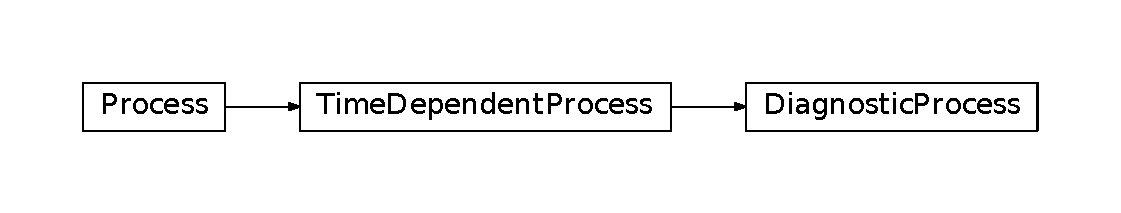
\includegraphics{inheritance-1888e33f5a851ed75afcf967b0ab7f3cd6fbbc2c.pdf}
\phantomsection\label{api/climlab.process:module-climlab.process.diagnostic}\index{climlab.process.diagnostic (module)}\index{DiagnosticProcess (class in climlab.process.diagnostic)}

\begin{fulllineitems}
\phantomsection\label{api/climlab.process:climlab.process.diagnostic.DiagnosticProcess}\pysiglinewithargsret{\strong{class }\code{climlab.process.diagnostic.}\bfcode{DiagnosticProcess}}{\emph{**kwargs}}{}
Bases: {\hyperref[api/climlab.process:climlab.process.time_dependent_process.TimeDependentProcess]{\emph{\code{climlab.process.time\_dependent\_process.TimeDependentProcess}}}} (\autopageref*{api/climlab.process:climlab.process.time_dependent_process.TimeDependentProcess})

A parent class for all processes that are strictly diagnostic, namely
no time dependence.

During initialization following attribute is set:
\begin{quote}\begin{description}
\item[{Variables}] \leavevmode
\textbf{\texttt{time\_type}} (\href{http://docs.python.org/2.7/library/functions.html\#str}{\emph{\texttt{str}}}) -- is set to \code{'diagnostic'}

\end{description}\end{quote}

\end{fulllineitems}



\subsubsection{climlab.process.energy\_budget module}
\label{api/climlab.process:climlab-process-energy-budget-module}
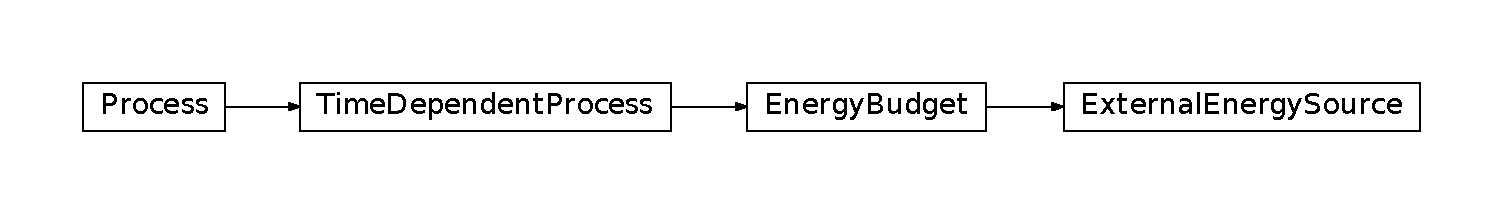
\includegraphics{inheritance-98fc96005ebee865666017a7ff9a04cb383ee609.pdf}
\phantomsection\label{api/climlab.process:module-climlab.process.energy_budget}\index{climlab.process.energy\_budget (module)}\index{EnergyBudget (class in climlab.process.energy\_budget)}

\begin{fulllineitems}
\phantomsection\label{api/climlab.process:climlab.process.energy_budget.EnergyBudget}\pysiglinewithargsret{\strong{class }\code{climlab.process.energy\_budget.}\bfcode{EnergyBudget}}{\emph{**kwargs}}{}
Bases: {\hyperref[api/climlab.process:climlab.process.time_dependent_process.TimeDependentProcess]{\emph{\code{climlab.process.time\_dependent\_process.TimeDependentProcess}}}} (\autopageref*{api/climlab.process:climlab.process.time_dependent_process.TimeDependentProcess})

A parent class for explicit energy budget processes.

This class solves equations that include a heat capacitiy term like
\(C \frac{dT}{dt} = \textrm{flux convergence}\)

In an Energy Balance Model with model state \(T\) this equation 
will look like this:
\begin{gather}
\begin{split}C \frac{dT}{dt} = R\downarrow - R\uparrow - H  \end{split}\notag\\\begin{split}\frac{dT}{dt} = \frac{R\downarrow}{C} - \frac{R\uparrow}{C} - \frac{H}{C}\end{split}\notag
\end{gather}
Every EnergyBudget object has a \code{heating\_rate} dictionary with items 
corresponding to each state variable. The heating rate accounts the actual 
heating of a subprocess, namely the contribution to the energy budget 
of \(R\downarrow, R\uparrow\) and \(H\) in this case.
The temperature tendencies for each subprocess are then calculated 
through dividing the heating rate by the heat capacitiy \(C\).

\textbf{Initialization parameters}

An instance of \code{EnergyBudget} is initialized with the forwarded 
keyword arguments \code{**kwargs} of the corresponding children classes.

\textbf{Object attributes}

Additional to the parent class 
\code{TimeDependentProcess}
following object attributes are generated or modified during initialization:
\begin{quote}\begin{description}
\item[{Variables}] \leavevmode\begin{itemize}
\item {} 
\textbf{\texttt{time\_type}} (\href{http://docs.python.org/2.7/library/functions.html\#str}{\emph{\texttt{str}}}) -- is set to \code{'explicit'}

\item {} 
\textbf{\texttt{heating\_rate}} (\href{http://docs.python.org/2.7/library/stdtypes.html\#dict}{\emph{\texttt{dict}}}) -- energy share for given subprocess in unit 
\(\textrm{W}/ \textrm{m}^2\) stored 
in a dictionary sorted by model states

\end{itemize}

\end{description}\end{quote}

\end{fulllineitems}

\index{ExternalEnergySource (class in climlab.process.energy\_budget)}

\begin{fulllineitems}
\phantomsection\label{api/climlab.process:climlab.process.energy_budget.ExternalEnergySource}\pysiglinewithargsret{\strong{class }\code{climlab.process.energy\_budget.}\bfcode{ExternalEnergySource}}{\emph{**kwargs}}{}
Bases: {\hyperref[api/climlab.process:climlab.process.energy_budget.EnergyBudget]{\emph{\code{climlab.process.energy\_budget.EnergyBudget}}}} (\autopageref*{api/climlab.process:climlab.process.energy_budget.EnergyBudget})

A fixed energy source or sink to be specified by the user.

\textbf{Object attributes}

Additional to the parent class {\hyperref[api/climlab.process:climlab.process.energy_budget.EnergyBudget]{\emph{\code{EnergyBudget}}}} (\autopageref*{api/climlab.process:climlab.process.energy_budget.EnergyBudget})
the following object attribute is modified during initialization:
\begin{quote}\begin{description}
\item[{Variables}] \leavevmode
\textbf{\texttt{heating\_rate}} (\href{http://docs.python.org/2.7/library/stdtypes.html\#dict}{\emph{\texttt{dict}}}) -- energy share dictionary for this subprocess
is set to zero for every model state.

\end{description}\end{quote}

After initialization the user should modify the fields in the 
\code{heating\_rate} dictionary, which contain heating rates in 
unit \(\textrm{W}/ \textrm{m}^2\) for all state variables.
\begin{quote}\begin{description}
\item[{Example}] \leavevmode
Creating an Energy Balance Model with a uniform external energy source
of \(10 \ \textrm{W}/ \textrm{m}^2\) for all latitudes:

\begin{Verbatim}[commandchars=\\\{\}]
\PYG{g+gp}{\PYGZgt{}\PYGZgt{}\PYGZgt{} }\PYG{k+kn}{import} \PYG{n+nn}{climlab}
\PYG{g+gp}{\PYGZgt{}\PYGZgt{}\PYGZgt{} }\PYG{k+kn}{from} \PYG{n+nn}{climlab.process.energy\PYGZus{}budget} \PYG{k+kn}{import} \PYG{n}{ExternalEnergySource}
\PYG{g+gp}{\PYGZgt{}\PYGZgt{}\PYGZgt{} }\PYG{k+kn}{import} \PYG{n+nn}{numpy} \PYG{k+kn}{as} \PYG{n+nn}{np}

\PYG{g+gp}{\PYGZgt{}\PYGZgt{}\PYGZgt{} }\PYG{c+c1}{\PYGZsh{} create model \PYGZam{} external energy subprocess}
\PYG{g+gp}{\PYGZgt{}\PYGZgt{}\PYGZgt{} }\PYG{n}{model} \PYG{o}{=} \PYG{n}{climlab}\PYG{o}{.}\PYG{n}{EBM}\PYG{p}{(}\PYG{n}{num\PYGZus{}lat}\PYG{o}{=}\PYG{l+m+mi}{36}\PYG{p}{)}
\PYG{g+gp}{\PYGZgt{}\PYGZgt{}\PYGZgt{} }\PYG{n}{ext\PYGZus{}en} \PYG{o}{=} \PYG{n}{ExternalEnergySource}\PYG{p}{(}\PYG{n}{state}\PYG{o}{=} \PYG{n}{model}\PYG{o}{.}\PYG{n}{state}\PYG{p}{,}\PYG{o}{*}\PYG{o}{*}\PYG{n}{model}\PYG{o}{.}\PYG{n}{param}\PYG{p}{)}

\PYG{g+gp}{\PYGZgt{}\PYGZgt{}\PYGZgt{} }\PYG{c+c1}{\PYGZsh{} modify external energy rate}
\PYG{g+gp}{\PYGZgt{}\PYGZgt{}\PYGZgt{} }\PYG{n}{ext\PYGZus{}en}\PYG{o}{.}\PYG{n}{heating\PYGZus{}rate}\PYG{o}{.}\PYG{n}{keys}\PYG{p}{(}\PYG{p}{)}
\PYG{g+go}{[\PYGZsq{}Ts\PYGZsq{}]}

\PYG{g+gp}{\PYGZgt{}\PYGZgt{}\PYGZgt{} }\PYG{n}{np}\PYG{o}{.}\PYG{n}{squeeze}\PYG{p}{(}\PYG{n}{ext\PYGZus{}en}\PYG{o}{.}\PYG{n}{heating\PYGZus{}rate}\PYG{p}{[}\PYG{l+s+s1}{\PYGZsq{}}\PYG{l+s+s1}{Ts}\PYG{l+s+s1}{\PYGZsq{}}\PYG{p}{]}\PYG{p}{)}
\PYG{g+go}{Field([\PYGZhy{}0., \PYGZhy{}0., \PYGZhy{}0., \PYGZhy{}0., \PYGZhy{}0., \PYGZhy{}0., \PYGZhy{}0., \PYGZhy{}0., \PYGZhy{}0.,  0.,  0.,  0.,  0.,}
\PYG{g+go}{        0.,  0.,  0.,  0.,  0.,  0.,  0.,  0.,  0.,  0.,  0.,  0.,  0.,}
\PYG{g+go}{        0., \PYGZhy{}0., \PYGZhy{}0., \PYGZhy{}0., \PYGZhy{}0., \PYGZhy{}0., \PYGZhy{}0., \PYGZhy{}0., \PYGZhy{}0., \PYGZhy{}0.])}

\PYG{g+gp}{\PYGZgt{}\PYGZgt{}\PYGZgt{} }\PYG{n}{ext\PYGZus{}en}\PYG{o}{.}\PYG{n}{heating\PYGZus{}rate}\PYG{p}{[}\PYG{l+s+s1}{\PYGZsq{}}\PYG{l+s+s1}{Ts}\PYG{l+s+s1}{\PYGZsq{}}\PYG{p}{]}\PYG{p}{[}\PYG{p}{:}\PYG{p}{]}\PYG{o}{=}\PYG{l+m+mi}{10}

\PYG{g+gp}{\PYGZgt{}\PYGZgt{}\PYGZgt{} }\PYG{n}{np}\PYG{o}{.}\PYG{n}{squeeze}\PYG{p}{(}\PYG{n}{ext\PYGZus{}en}\PYG{o}{.}\PYG{n}{heating\PYGZus{}rate}\PYG{p}{[}\PYG{l+s+s1}{\PYGZsq{}}\PYG{l+s+s1}{Ts}\PYG{l+s+s1}{\PYGZsq{}}\PYG{p}{]}\PYG{p}{)}
\PYG{g+go}{Field([ 10.,  10.,  10.,  10.,  10.,  10.,  10.,  10.,  10.,  10.,  10.,}
\PYG{g+go}{        10.,  10.,  10.,  10.,  10.,  10.,  10.,  10.,  10.,  10.,  10.,}
\PYG{g+go}{        10.,  10.,  10.,  10.,  10.,  10.,  10.,  10.,  10.,  10.,  10.,}
\PYG{g+go}{        10.,  10.,  10.])}

\PYG{g+gp}{\PYGZgt{}\PYGZgt{}\PYGZgt{} }\PYG{c+c1}{\PYGZsh{} add subprocess to model}
\PYG{g+gp}{\PYGZgt{}\PYGZgt{}\PYGZgt{} }\PYG{n}{model}\PYG{o}{.}\PYG{n}{add\PYGZus{}subprocess}\PYG{p}{(}\PYG{l+s+s1}{\PYGZsq{}}\PYG{l+s+s1}{ext\PYGZus{}energy}\PYG{l+s+s1}{\PYGZsq{}}\PYG{p}{,}\PYG{n}{ext\PYGZus{}en}\PYG{p}{)}

\PYG{g+gp}{\PYGZgt{}\PYGZgt{}\PYGZgt{} }\PYG{k}{print} \PYG{n}{model}
\PYG{g+go}{climlab Process of type \PYGZlt{}class \PYGZsq{}climlab.model.ebm.EBM\PYGZsq{}\PYGZgt{}. }
\PYG{g+go}{State variables and domain shapes: }
\PYG{g+go}{  Ts: (36, 1) }
\PYG{g+go}{The subprocess tree: }
\PYG{g+go}{top: \PYGZlt{}class \PYGZsq{}climlab.model.ebm.EBM\PYGZsq{}\PYGZgt{}}
\PYG{g+go}{   diffusion: \PYGZlt{}class \PYGZsq{}climlab.dynamics.diffusion.MeridionalDiffusion\PYGZsq{}\PYGZgt{}}
\PYG{g+go}{   LW: \PYGZlt{}class \PYGZsq{}climlab.radiation.AplusBT.AplusBT\PYGZsq{}\PYGZgt{}}
\PYG{g+go}{   ext\PYGZus{}energy: \PYGZlt{}class \PYGZsq{}climlab.process.energy\PYGZus{}budget.ExternalEnergySource\PYGZsq{}\PYGZgt{}}
\PYG{g+go}{   albedo: \PYGZlt{}class \PYGZsq{}climlab.surface.albedo.StepFunctionAlbedo\PYGZsq{}\PYGZgt{}}
\PYG{g+go}{      iceline: \PYGZlt{}class \PYGZsq{}climlab.surface.albedo.Iceline\PYGZsq{}\PYGZgt{}}
\PYG{g+go}{      cold\PYGZus{}albedo: \PYGZlt{}class \PYGZsq{}climlab.surface.albedo.ConstantAlbedo\PYGZsq{}\PYGZgt{}}
\PYG{g+go}{      warm\PYGZus{}albedo: \PYGZlt{}class \PYGZsq{}climlab.surface.albedo.P2Albedo\PYGZsq{}\PYGZgt{}}
\PYG{g+go}{   insolation: \PYGZlt{}class \PYGZsq{}climlab.radiation.insolation.P2Insolation\PYGZsq{}\PYGZgt{}}
\end{Verbatim}

\end{description}\end{quote}

\end{fulllineitems}



\subsubsection{climlab.process.implicit module}
\label{api/climlab.process:climlab-process-implicit-module}
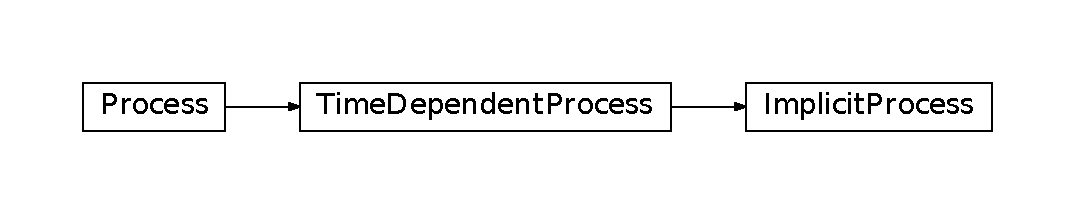
\includegraphics{inheritance-0ec5e793f32d044b3bed47f7343a17291cc60065.pdf}
\phantomsection\label{api/climlab.process:module-climlab.process.implicit}\index{climlab.process.implicit (module)}\index{ImplicitProcess (class in climlab.process.implicit)}

\begin{fulllineitems}
\phantomsection\label{api/climlab.process:climlab.process.implicit.ImplicitProcess}\pysiglinewithargsret{\strong{class }\code{climlab.process.implicit.}\bfcode{ImplicitProcess}}{\emph{**kwargs}}{}
Bases: {\hyperref[api/climlab.process:climlab.process.time_dependent_process.TimeDependentProcess]{\emph{\code{climlab.process.time\_dependent\_process.TimeDependentProcess}}}} (\autopageref*{api/climlab.process:climlab.process.time_dependent_process.TimeDependentProcess})

A parent class for modules that use implicit time discretization.

During initialization following attributes are intitialized:
\begin{quote}\begin{description}
\item[{Variables}] \leavevmode\begin{itemize}
\item {} 
\textbf{\texttt{time\_type}} (\href{http://docs.python.org/2.7/library/functions.html\#str}{\emph{\texttt{str}}}) -- is set to \code{'implicit'}

\item {} 
\textbf{\texttt{adjustment}} (\href{http://docs.python.org/2.7/library/stdtypes.html\#dict}{\emph{\texttt{dict}}}) -- the model state adjustments due to this implicit 
subprocess

\end{itemize}

\end{description}\end{quote}
\index{\_compute() (climlab.process.implicit.ImplicitProcess method)}

\begin{fulllineitems}
\phantomsection\label{api/climlab.process:climlab.process.implicit.ImplicitProcess._compute}\pysiglinewithargsret{\bfcode{\_compute}}{}{}
Computes the state variable tendencies in time for implicit processes.

To calculate the new state the \code{\_implicit\_solver()} method is 
called for daughter classes. This however returns the new state of the 
variables, not just the tendencies. Therefore, the adjustment is 
calculated which is the difference between the new and the old state 
and stored in the object's attribute adjustment.

Calculating the new model states through solving the matrix problem 
already includes the multiplication with the timestep. The derived 
adjustment is divided by the timestep to calculate the implicit 
subprocess tendencies, which can be handeled by the 
{\hyperref[api/climlab.process:climlab.process.time_dependent_process.TimeDependentProcess.compute]{\emph{\code{compute()}}}} (\autopageref*{api/climlab.process:climlab.process.time_dependent_process.TimeDependentProcess.compute})
method of the parent 
{\hyperref[api/climlab.process:climlab.process.time_dependent_process.TimeDependentProcess]{\emph{\code{TimeDependentProcess}}}} (\autopageref*{api/climlab.process:climlab.process.time_dependent_process.TimeDependentProcess}) class.
\begin{quote}\begin{description}
\item[{Variables}] \leavevmode
\textbf{\texttt{adjustment}} (\href{http://docs.python.org/2.7/library/stdtypes.html\#dict}{\emph{\texttt{dict}}}) -- holding all state variables' adjustments
of the implicit process which are the 
differences between the new states (which have 
been solved through matrix inversion) and the 
old states.

\end{description}\end{quote}

\end{fulllineitems}


\end{fulllineitems}



\subsubsection{climlab.process.process module}
\label{api/climlab.process:climlab-process-process-module}
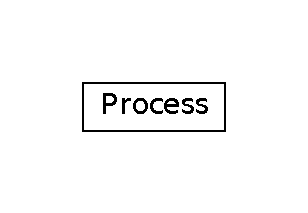
\includegraphics{inheritance-8eb24c41e1d3c85885c11e2e65fb208089ce0aa8.pdf}
\phantomsection\label{api/climlab.process:module-climlab.process.process}\index{climlab.process.process (module)}\index{Process (class in climlab.process.process)}

\begin{fulllineitems}
\phantomsection\label{api/climlab.process:climlab.process.process.Process}\pysiglinewithargsret{\strong{class }\code{climlab.process.process.}\bfcode{Process}}{\emph{state=None}, \emph{domains=None}, \emph{subprocess=None}, \emph{lat=None}, \emph{lev=None}, \emph{num\_lat=None}, \emph{num\_levels=None}, \emph{input=None}, \emph{**kwargs}}{}
Bases: \href{http://docs.python.org/2.7/library/functions.html\#object}{\code{object}}

A generic parent class for all climlab process objects.
Every process object has a set of state variables on a spatial grid.

For more general information about \emph{Processes} and their role in climlab,
see {\hyperref[architecture:process\string-architecture]{\emph{Process}}} (\autopageref*{architecture:process-architecture}) section climlab-architecture.

\textbf{Initialization parameters}

An instance of \code{Process} is initialized with the following 
arguments \emph{(for detailed information see Object attributes below)}:
\begin{quote}\begin{description}
\item[{Parameters}] \leavevmode\begin{itemize}
\item {} 
\textbf{\texttt{state}} ({\hyperref[api/climlab.domain:climlab.domain.field.Field]{\emph{\emph{\texttt{Field}}}}} (\autopageref*{api/climlab.domain:climlab.domain.field.Field})) -- spatial state variable for the process. 
Set to \code{None} if not specified.

\item {} 
\textbf{\texttt{domains}} ({\hyperref[api/climlab.domain:climlab.domain.domain._Domain]{\emph{\code{\_Domain}}}} (\autopageref*{api/climlab.domain:climlab.domain.domain._Domain}) or dict of 
{\hyperref[api/climlab.domain:climlab.domain.domain._Domain]{\emph{\code{\_Domain}}}} (\autopageref*{api/climlab.domain:climlab.domain.domain._Domain})) -- domain(s) for the process

\item {} 
\textbf{\texttt{subprocess}} ({\hyperref[api/climlab.process:climlab.process.process.Process]{\emph{\code{Process}}}} (\autopageref*{api/climlab.process:climlab.process.process.Process}) or dict of 
{\hyperref[api/climlab.process:climlab.process.process.Process]{\emph{\code{Process}}}} (\autopageref*{api/climlab.process:climlab.process.process.Process})) -- subprocess(es) of the process

\item {} 
\textbf{\texttt{lat}} (\href{http://docs.python.org/2.7/library/array.html\#module-array}{\emph{\texttt{array}}}) -- latitudinal points (optional)

\item {} 
\textbf{\texttt{lev}} -- altitudinal points (optional)

\item {} 
\textbf{\texttt{num\_lat}} (\href{http://docs.python.org/2.7/library/functions.html\#int}{\emph{\texttt{int}}}) -- number of latitudional points (optional)

\item {} 
\textbf{\texttt{num\_levels}} (\href{http://docs.python.org/2.7/library/functions.html\#int}{\emph{\texttt{int}}}) -- number of altitudinal points (optional)

\item {} 
\textbf{\texttt{input}} (\href{http://docs.python.org/2.7/library/stdtypes.html\#dict}{\emph{\texttt{dict}}}) -- collection of input quantities

\end{itemize}

\end{description}\end{quote}

\textbf{Object attributes}

Additional to the parent class {\hyperref[api/climlab.process:climlab.process.process.Process]{\emph{\code{Process}}}} (\autopageref*{api/climlab.process:climlab.process.process.Process})
following object attributes are generated during initialization:
\begin{quote}\begin{description}
\item[{Variables}] \leavevmode\begin{itemize}
\item {} 
\textbf{\texttt{domains}} (\href{http://docs.python.org/2.7/library/stdtypes.html\#dict}{\emph{\texttt{dict}}}) -- dictionary of process {\hyperref[api/climlab.domain:climlab.domain.domain._Domain]{\emph{\code{\_Domain}}}} (\autopageref*{api/climlab.domain:climlab.domain.domain._Domain})

\item {} 
\textbf{\texttt{state}} (\href{http://docs.python.org/2.7/library/stdtypes.html\#dict}{\emph{\texttt{dict}}}) -- dictionary of process states 
(of type {\hyperref[api/climlab.domain:climlab.domain.field.Field]{\emph{\code{Field}}}} (\autopageref*{api/climlab.domain:climlab.domain.field.Field}))

\item {} 
\textbf{\texttt{param}} (\href{http://docs.python.org/2.7/library/stdtypes.html\#dict}{\emph{\texttt{dict}}}) -- dictionary of model parameters which are given
through \code{**kwargs}

\item {} 
\textbf{\texttt{diagnostics}} (\href{http://docs.python.org/2.7/library/stdtypes.html\#dict}{\emph{\texttt{dict}}}) -- a dictionary with all diagnostic variables

\item {} 
\textbf{\texttt{\_input\_vars}} (\href{http://docs.python.org/2.7/library/stdtypes.html\#dict}{\emph{\texttt{dict}}}) -- collection of input quantities like boundary conditions
and other gridded quantities

\item {} 
\textbf{\texttt{creation\_date}} (\href{http://docs.python.org/2.7/library/functions.html\#str}{\emph{\texttt{str}}}) -- date and time when process was created

\item {} 
\href{http://docs.python.org/2.7/library/subprocess.html\#module-subprocess}{\textbf{\texttt{subprocess}}} (dict of {\hyperref[api/climlab.process:climlab.process.process.Process]{\emph{\code{Process}}}} (\autopageref*{api/climlab.process:climlab.process.process.Process})) -- dictionary of suprocesses of the process

\end{itemize}

\end{description}\end{quote}
\index{add\_input() (climlab.process.process.Process method)}

\begin{fulllineitems}
\phantomsection\label{api/climlab.process:climlab.process.process.Process.add_input}\pysiglinewithargsret{\bfcode{add\_input}}{\emph{inputlist}}{}
Updates the process's list of inputs.
\begin{quote}\begin{description}
\item[{Parameters}] \leavevmode
\textbf{\texttt{inputlist}} (\href{http://docs.python.org/2.7/library/functions.html\#list}{\emph{\texttt{list}}}) -- list of names of input variables

\end{description}\end{quote}

\end{fulllineitems}

\index{add\_subprocess() (climlab.process.process.Process method)}

\begin{fulllineitems}
\phantomsection\label{api/climlab.process:climlab.process.process.Process.add_subprocess}\pysiglinewithargsret{\bfcode{add\_subprocess}}{\emph{name}, \emph{proc}}{}
Adds a single subprocess to this process.
\begin{quote}\begin{description}
\item[{Parameters}] \leavevmode\begin{itemize}
\item {} 
\textbf{\texttt{name}} (\href{http://docs.python.org/2.7/library/string.html\#module-string}{\emph{\texttt{string}}}) -- name of the subprocess

\item {} 
\textbf{\texttt{proc}} ({\hyperref[api/climlab.process:climlab.process.process.Process]{\emph{\code{Process}}}} (\autopageref*{api/climlab.process:climlab.process.process.Process})) -- a Process object

\end{itemize}

\item[{Raises}] \leavevmode
\code{ValueError} 
if \code{proc} is not a process

\item[{Example}] \leavevmode
Replacing an albedo subprocess through adding a subprocess with 
same name:

\begin{Verbatim}[commandchars=\\\{\}]
\PYG{g+gp}{\PYGZgt{}\PYGZgt{}\PYGZgt{} }\PYG{k+kn}{from} \PYG{n+nn}{climlab.model.ebm} \PYG{k+kn}{import} \PYG{n}{EBM\PYGZus{}seasonal}
\PYG{g+gp}{\PYGZgt{}\PYGZgt{}\PYGZgt{} }\PYG{k+kn}{from} \PYG{n+nn}{climlab.surface.albedo} \PYG{k+kn}{import} \PYG{n}{StepFunctionAlbedo}

\PYG{g+gp}{\PYGZgt{}\PYGZgt{}\PYGZgt{} }\PYG{c+c1}{\PYGZsh{} creating EBM model}
\PYG{g+gp}{\PYGZgt{}\PYGZgt{}\PYGZgt{} }\PYG{n}{ebm\PYGZus{}s} \PYG{o}{=} \PYG{n}{EBM\PYGZus{}seasonal}\PYG{p}{(}\PYG{p}{)}

\PYG{g+gp}{\PYGZgt{}\PYGZgt{}\PYGZgt{} }\PYG{k}{print} \PYG{n}{ebm\PYGZus{}s}
\end{Verbatim}

\begin{Verbatim}[commandchars=\\\{\}]
climlab Process of type \PYGZlt{}class \PYGZsq{}climlab.model.ebm.EBM\PYGZus{}seasonal\PYGZsq{}\PYGZgt{}. 
State variables and domain shapes: 
  Ts: (90, 1) 
The subprocess tree: 
top: \PYGZlt{}class \PYGZsq{}climlab.model.ebm.EBM\PYGZus{}seasonal\PYGZsq{}\PYGZgt{}
   diffusion: \PYGZlt{}class \PYGZsq{}climlab.dynamics.diffusion.MeridionalDiffusion\PYGZsq{}\PYGZgt{}
   LW: \PYGZlt{}class \PYGZsq{}climlab.radiation.AplusBT.AplusBT\PYGZsq{}\PYGZgt{}
   albedo: \PYGZlt{}class \PYGZsq{}climlab.surface.albedo.P2Albedo\PYGZsq{}\PYGZgt{}
   insolation: \PYGZlt{}class \PYGZsq{}climlab.radiation.insolation.DailyInsolation\PYGZsq{}\PYGZgt{}
\end{Verbatim}

\begin{Verbatim}[commandchars=\\\{\}]
\PYG{g+gp}{\PYGZgt{}\PYGZgt{}\PYGZgt{} }\PYG{c+c1}{\PYGZsh{}  creating and adding albedo feedback subprocess}
\PYG{g+gp}{\PYGZgt{}\PYGZgt{}\PYGZgt{} }\PYG{n}{step\PYGZus{}albedo} \PYG{o}{=} \PYG{n}{StepFunctionAlbedo}\PYG{p}{(}\PYG{n}{state}\PYG{o}{=}\PYG{n}{ebm\PYGZus{}s}\PYG{o}{.}\PYG{n}{state}\PYG{p}{,} \PYG{o}{*}\PYG{o}{*}\PYG{n}{ebm\PYGZus{}s}\PYG{o}{.}\PYG{n}{param}\PYG{p}{)}
\PYG{g+gp}{\PYGZgt{}\PYGZgt{}\PYGZgt{} }\PYG{n}{ebm\PYGZus{}s}\PYG{o}{.}\PYG{n}{add\PYGZus{}subprocess}\PYG{p}{(}\PYG{l+s+s1}{\PYGZsq{}}\PYG{l+s+s1}{albedo}\PYG{l+s+s1}{\PYGZsq{}}\PYG{p}{,} \PYG{n}{step\PYGZus{}albedo}\PYG{p}{)}
\PYG{g+gp}{\PYGZgt{}\PYGZgt{}\PYGZgt{} }
\PYG{g+gp}{\PYGZgt{}\PYGZgt{}\PYGZgt{} }\PYG{k}{print} \PYG{n}{ebm\PYGZus{}s}
\end{Verbatim}

\begin{Verbatim}[commandchars=\\\{\}]
climlab Process of type \PYGZlt{}class \PYGZsq{}climlab.model.ebm.EBM\PYGZus{}seasonal\PYGZsq{}\PYGZgt{}. 
State variables and domain shapes: 
  Ts: (90, 1) 
The subprocess tree: 
top: \PYGZlt{}class \PYGZsq{}climlab.model.ebm.EBM\PYGZus{}seasonal\PYGZsq{}\PYGZgt{}
   diffusion: \PYGZlt{}class \PYGZsq{}climlab.dynamics.diffusion.MeridionalDiffusion\PYGZsq{}\PYGZgt{}
   LW: \PYGZlt{}class \PYGZsq{}climlab.radiation.AplusBT.AplusBT\PYGZsq{}\PYGZgt{}
   albedo: \PYGZlt{}class \PYGZsq{}climlab.surface.albedo.StepFunctionAlbedo\PYGZsq{}\PYGZgt{}
      iceline: \PYGZlt{}class \PYGZsq{}climlab.surface.albedo.Iceline\PYGZsq{}\PYGZgt{}
      cold\PYGZus{}albedo: \PYGZlt{}class \PYGZsq{}climlab.surface.albedo.ConstantAlbedo\PYGZsq{}\PYGZgt{}
      warm\PYGZus{}albedo: \PYGZlt{}class \PYGZsq{}climlab.surface.albedo.P2Albedo\PYGZsq{}\PYGZgt{}
   insolation: \PYGZlt{}class \PYGZsq{}climlab.radiation.insolation.DailyInsolation\PYGZsq{}\PYGZgt{}
\end{Verbatim}

\end{description}\end{quote}

\end{fulllineitems}

\index{add\_subprocesses() (climlab.process.process.Process method)}

\begin{fulllineitems}
\phantomsection\label{api/climlab.process:climlab.process.process.Process.add_subprocesses}\pysiglinewithargsret{\bfcode{add\_subprocesses}}{\emph{procdict}}{}
Adds a dictionary of subproceses to this process.

Calls {\hyperref[api/climlab.process:climlab.process.process.Process.add_subprocess]{\emph{\code{add\_subprocess()}}}} (\autopageref*{api/climlab.process:climlab.process.process.Process.add_subprocess}) for every process given in the 
input-dictionary. It can also pass a single process, which will 
be given the name \emph{default}.
\begin{quote}\begin{description}
\item[{Parameters}] \leavevmode
\textbf{\texttt{procdict}} (\href{http://docs.python.org/2.7/library/stdtypes.html\#dict}{\emph{\texttt{dict}}}) -- a dictionary with process names as keys

\end{description}\end{quote}

\end{fulllineitems}

\index{depth (climlab.process.process.Process attribute)}

\begin{fulllineitems}
\phantomsection\label{api/climlab.process:climlab.process.process.Process.depth}\pysigline{\bfcode{depth}}
Property of depth points of the process.
\begin{quote}\begin{description}
\item[{Getter}] \leavevmode
Returns the points of axis \code{'depth'} if availible in the
process's domains.

\item[{Type}] \leavevmode
array

\item[{Raises}] \leavevmode
\code{ValueError}
if no \code{'depth'} axis can be found.

\end{description}\end{quote}

\end{fulllineitems}

\index{depth\_bounds (climlab.process.process.Process attribute)}

\begin{fulllineitems}
\phantomsection\label{api/climlab.process:climlab.process.process.Process.depth_bounds}\pysigline{\bfcode{depth\_bounds}}
Property of depth bounds of the process.
\begin{quote}\begin{description}
\item[{Getter}] \leavevmode
Returns the bounds of axis \code{'depth'} if availible in the
process's domains.

\item[{Type}] \leavevmode
array

\item[{Raises}] \leavevmode
\code{ValueError}
if no \code{'depth'} axis can be found.

\end{description}\end{quote}

\end{fulllineitems}

\index{init\_diagnostic() (climlab.process.process.Process method)}

\begin{fulllineitems}
\phantomsection\label{api/climlab.process:climlab.process.process.Process.init_diagnostic}\pysiglinewithargsret{\bfcode{init\_diagnostic}}{\emph{name}, \emph{value=0.0}}{}
Defines a new diagnostic quantity called \code{name}
and initialize it with the given \code{value}.

Quantity is accessible and settable in two ways:
\begin{itemize}
\item {} 
as a process attribute, i.e. \code{proc.name}

\item {} 
as a member of the diagnostics dictionary, 
i.e. \code{proc.diagnostics{[}'name'{]}}

\end{itemize}
\begin{quote}\begin{description}
\item[{Parameters}] \leavevmode\begin{itemize}
\item {} 
\textbf{\texttt{name}} (\href{http://docs.python.org/2.7/library/functions.html\#str}{\emph{\texttt{str}}}) -- name of diagnostic quantity to be initialized

\item {} 
\textbf{\texttt{value}} (\href{http://docs.python.org/2.7/library/array.html\#module-array}{\emph{\texttt{array}}}) -- initial value for quantity - accepts also type
float, int, etc. {[}default: 0.{]}

\end{itemize}

\item[{Example}] \leavevmode
Add a diagnostic CO2 variable to an energy balance model:

\begin{Verbatim}[commandchars=\\\{\}]
\PYG{g+gp}{\PYGZgt{}\PYGZgt{}\PYGZgt{} }\PYG{k+kn}{import} \PYG{n+nn}{climlab}
\PYG{g+gp}{\PYGZgt{}\PYGZgt{}\PYGZgt{} }\PYG{n}{model} \PYG{o}{=} \PYG{n}{climlab}\PYG{o}{.}\PYG{n}{EBM}\PYG{p}{(}\PYG{p}{)}

\PYG{g+gp}{\PYGZgt{}\PYGZgt{}\PYGZgt{} }\PYG{c+c1}{\PYGZsh{} initialize CO2 variable with value 280 ppm}
\PYG{g+gp}{\PYGZgt{}\PYGZgt{}\PYGZgt{} }\PYG{n}{model}\PYG{o}{.}\PYG{n}{init\PYGZus{}diagnostic}\PYG{p}{(}\PYG{l+s+s1}{\PYGZsq{}}\PYG{l+s+s1}{CO2}\PYG{l+s+s1}{\PYGZsq{}}\PYG{p}{,}\PYG{l+m+mi}{280}\PYG{p}{)}

\PYG{g+gp}{\PYGZgt{}\PYGZgt{}\PYGZgt{} }\PYG{c+c1}{\PYGZsh{} access variable directly or through diagnostic dictionary}
\PYG{g+gp}{\PYGZgt{}\PYGZgt{}\PYGZgt{} }\PYG{n}{model}\PYG{o}{.}\PYG{n}{CO2}
\PYG{g+go}{280}
\PYG{g+gp}{\PYGZgt{}\PYGZgt{}\PYGZgt{} }\PYG{n}{model}\PYG{o}{.}\PYG{n}{diagnostics}\PYG{o}{.}\PYG{n}{keys}\PYG{p}{(}\PYG{p}{)}
\PYG{g+go}{[\PYGZsq{}ASR\PYGZsq{}, \PYGZsq{}CO2\PYGZsq{}, \PYGZsq{}net\PYGZus{}radiation\PYGZsq{}, \PYGZsq{}icelat\PYGZsq{}, \PYGZsq{}OLR\PYGZsq{}, \PYGZsq{}albedo\PYGZsq{}]}
\end{Verbatim}

\end{description}\end{quote}

\end{fulllineitems}

\index{input (climlab.process.process.Process attribute)}

\begin{fulllineitems}
\phantomsection\label{api/climlab.process:climlab.process.process.Process.input}\pysigline{\bfcode{input}}
dictionary with all input variables

That can be boundary conditions and other gridded quantities 
independent of the \emph{process}
\begin{quote}\begin{description}
\item[{Getter}] \leavevmode
Returns the content of \code{self.\_input\_vars}.

\item[{Type}] \leavevmode
dict

\end{description}\end{quote}

\end{fulllineitems}

\index{lat (climlab.process.process.Process attribute)}

\begin{fulllineitems}
\phantomsection\label{api/climlab.process:climlab.process.process.Process.lat}\pysigline{\bfcode{lat}}
Property of latitudinal points of the process.
\begin{quote}\begin{description}
\item[{Getter}] \leavevmode
Returns the points of axis \code{'lat'} if availible in the
process's domains.

\item[{Type}] \leavevmode
array

\item[{Raises}] \leavevmode
\code{ValueError}
if no \code{'lat'} axis can be found.

\end{description}\end{quote}

\end{fulllineitems}

\index{lat\_bounds (climlab.process.process.Process attribute)}

\begin{fulllineitems}
\phantomsection\label{api/climlab.process:climlab.process.process.Process.lat_bounds}\pysigline{\bfcode{lat\_bounds}}
Property of latitudinal bounds of the process.
\begin{quote}\begin{description}
\item[{Getter}] \leavevmode
Returns the bounds of axis \code{'lat'} if availible in the
process's domains.

\item[{Type}] \leavevmode
array

\item[{Raises}] \leavevmode
\code{ValueError}
if no \code{'lat'} axis can be found.

\end{description}\end{quote}

\end{fulllineitems}

\index{lev (climlab.process.process.Process attribute)}

\begin{fulllineitems}
\phantomsection\label{api/climlab.process:climlab.process.process.Process.lev}\pysigline{\bfcode{lev}}
Property of altitudinal points of the process.
\begin{quote}\begin{description}
\item[{Getter}] \leavevmode
Returns the points of axis \code{'lev'} if availible in the
process's domains.

\item[{Type}] \leavevmode
array

\item[{Raises}] \leavevmode
\code{ValueError}
if no \code{'lev'} axis can be found.

\end{description}\end{quote}

\end{fulllineitems}

\index{lev\_bounds (climlab.process.process.Process attribute)}

\begin{fulllineitems}
\phantomsection\label{api/climlab.process:climlab.process.process.Process.lev_bounds}\pysigline{\bfcode{lev\_bounds}}
Property of altitudinal bounds of the process.
\begin{quote}\begin{description}
\item[{Getter}] \leavevmode
Returns the bounds of axis \code{'lev'} if availible in the
process's domains.

\item[{Type}] \leavevmode
array

\item[{Raises}] \leavevmode
\code{ValueError}
if no \code{'lev'} axis can be found.

\end{description}\end{quote}

\end{fulllineitems}

\index{lon (climlab.process.process.Process attribute)}

\begin{fulllineitems}
\phantomsection\label{api/climlab.process:climlab.process.process.Process.lon}\pysigline{\bfcode{lon}}
Property of longitudinal points of the process.
\begin{quote}\begin{description}
\item[{Getter}] \leavevmode
Returns the points of axis \code{'lon'} if availible in the
process's domains.

\item[{Type}] \leavevmode
array

\item[{Raises}] \leavevmode
\code{ValueError}
if no \code{'lon'} axis can be found.

\end{description}\end{quote}

\end{fulllineitems}

\index{lon\_bounds (climlab.process.process.Process attribute)}

\begin{fulllineitems}
\phantomsection\label{api/climlab.process:climlab.process.process.Process.lon_bounds}\pysigline{\bfcode{lon\_bounds}}
Property of longitudinal bounds of the process.
\begin{quote}\begin{description}
\item[{Getter}] \leavevmode
Returns the bounds of axis \code{'lon'} if availible in the
process's domains.

\item[{Type}] \leavevmode
array

\item[{Raises}] \leavevmode
\code{ValueError}
if no \code{'lon'} axis can be found.

\end{description}\end{quote}

\end{fulllineitems}

\index{remove\_diagnostic() (climlab.process.process.Process method)}

\begin{fulllineitems}
\phantomsection\label{api/climlab.process:climlab.process.process.Process.remove_diagnostic}\pysiglinewithargsret{\bfcode{remove\_diagnostic}}{\emph{name}}{}
Removes a diagnostic from the \code{process.diagnostic} dictionary
and also delete the associated process attribute.
\begin{quote}\begin{description}
\item[{Parameters}] \leavevmode
\textbf{\texttt{name}} (\href{http://docs.python.org/2.7/library/functions.html\#str}{\emph{\texttt{str}}}) -- name of diagnostic quantity to be removed

\item[{Example}] \leavevmode
Remove diagnostic variable `icelat' from energy balance model:

\begin{Verbatim}[commandchars=\\\{\}]
\PYG{g+gp}{\PYGZgt{}\PYGZgt{}\PYGZgt{} }\PYG{k+kn}{import} \PYG{n+nn}{climlab}
\PYG{g+gp}{\PYGZgt{}\PYGZgt{}\PYGZgt{} }\PYG{n}{model} \PYG{o}{=} \PYG{n}{climlab}\PYG{o}{.}\PYG{n}{EBM}\PYG{p}{(}\PYG{p}{)}

\PYG{g+gp}{\PYGZgt{}\PYGZgt{}\PYGZgt{} }\PYG{c+c1}{\PYGZsh{} display all diagnostic variables}
\PYG{g+gp}{\PYGZgt{}\PYGZgt{}\PYGZgt{} }\PYG{n}{model}\PYG{o}{.}\PYG{n}{diagnostics}\PYG{o}{.}\PYG{n}{keys}\PYG{p}{(}\PYG{p}{)}
\PYG{g+go}{[\PYGZsq{}ASR\PYGZsq{}, \PYGZsq{}OLR\PYGZsq{}, \PYGZsq{}net\PYGZus{}radiation\PYGZsq{}, \PYGZsq{}albedo\PYGZsq{}, \PYGZsq{}icelat\PYGZsq{}]}

\PYG{g+gp}{\PYGZgt{}\PYGZgt{}\PYGZgt{} }\PYG{n}{model}\PYG{o}{.}\PYG{n}{remove\PYGZus{}diagnostic}\PYG{p}{(}\PYG{l+s+s1}{\PYGZsq{}}\PYG{l+s+s1}{icelat}\PYG{l+s+s1}{\PYGZsq{}}\PYG{p}{)}
\PYG{g+gp}{\PYGZgt{}\PYGZgt{}\PYGZgt{} }\PYG{n}{model}\PYG{o}{.}\PYG{n}{diagnostics}\PYG{o}{.}\PYG{n}{keys}\PYG{p}{(}\PYG{p}{)}
\PYG{g+go}{[\PYGZsq{}ASR\PYGZsq{}, \PYGZsq{}OLR\PYGZsq{}, \PYGZsq{}net\PYGZus{}radiation\PYGZsq{}, \PYGZsq{}albedo\PYGZsq{}]}

\PYG{g+gp}{\PYGZgt{}\PYGZgt{}\PYGZgt{} }\PYG{c+c1}{\PYGZsh{} Watch out for subprocesses that may still want }
\PYG{g+gp}{\PYGZgt{}\PYGZgt{}\PYGZgt{} } \PYG{c+c1}{\PYGZsh{} to access the diagnostic \PYGZsq{}icelat\PYGZsq{} variable !!!}
\end{Verbatim}

\end{description}\end{quote}

\end{fulllineitems}

\index{remove\_subprocess() (climlab.process.process.Process method)}

\begin{fulllineitems}
\phantomsection\label{api/climlab.process:climlab.process.process.Process.remove_subprocess}\pysiglinewithargsret{\bfcode{remove\_subprocess}}{\emph{name}}{}
Removes a single subprocess from this process.
\begin{quote}\begin{description}
\item[{Parameters}] \leavevmode
\textbf{\texttt{name}} (\href{http://docs.python.org/2.7/library/string.html\#module-string}{\emph{\texttt{string}}}) -- name of the subprocess

\item[{Example}] \leavevmode
Remove albedo subprocess from energy balance model:

\begin{Verbatim}[commandchars=\\\{\}]
\PYG{g+gp}{\PYGZgt{}\PYGZgt{}\PYGZgt{} }\PYG{k+kn}{import} \PYG{n+nn}{climlab}
\PYG{g+gp}{\PYGZgt{}\PYGZgt{}\PYGZgt{} }\PYG{n}{model} \PYG{o}{=} \PYG{n}{climlab}\PYG{o}{.}\PYG{n}{EBM}\PYG{p}{(}\PYG{p}{)}

\PYG{g+gp}{\PYGZgt{}\PYGZgt{}\PYGZgt{} }\PYG{k}{print} \PYG{n}{model}
\PYG{g+go}{climlab Process of type \PYGZlt{}class \PYGZsq{}climlab.model.ebm.EBM\PYGZsq{}\PYGZgt{}. }
\PYG{g+go}{State variables and domain shapes: }
\PYG{g+go}{  Ts: (90, 1) }
\PYG{g+go}{The subprocess tree: }
\PYG{g+go}{top: \PYGZlt{}class \PYGZsq{}climlab.model.ebm.EBM\PYGZsq{}\PYGZgt{}}
\PYG{g+go}{   diffusion: \PYGZlt{}class \PYGZsq{}climlab.dynamics.diffusion.MeridionalDiffusion\PYGZsq{}\PYGZgt{}}
\PYG{g+go}{   LW: \PYGZlt{}class \PYGZsq{}climlab.radiation.AplusBT.AplusBT\PYGZsq{}\PYGZgt{}}
\PYG{g+go}{   albedo: \PYGZlt{}class \PYGZsq{}climlab.surface.albedo.StepFunctionAlbedo\PYGZsq{}\PYGZgt{}}
\PYG{g+go}{      iceline: \PYGZlt{}class \PYGZsq{}climlab.surface.albedo.Iceline\PYGZsq{}\PYGZgt{}}
\PYG{g+go}{      cold\PYGZus{}albedo: \PYGZlt{}class \PYGZsq{}climlab.surface.albedo.ConstantAlbedo\PYGZsq{}\PYGZgt{}}
\PYG{g+go}{      warm\PYGZus{}albedo: \PYGZlt{}class \PYGZsq{}climlab.surface.albedo.P2Albedo\PYGZsq{}\PYGZgt{}}
\PYG{g+go}{   insolation: \PYGZlt{}class \PYGZsq{}climlab.radiation.insolation.P2Insolation\PYGZsq{}\PYGZgt{}}

\PYG{g+gp}{\PYGZgt{}\PYGZgt{}\PYGZgt{} }\PYG{n}{model}\PYG{o}{.}\PYG{n}{remove\PYGZus{}subprocess}\PYG{p}{(}\PYG{l+s+s1}{\PYGZsq{}}\PYG{l+s+s1}{albedo}\PYG{l+s+s1}{\PYGZsq{}}\PYG{p}{)}

\PYG{g+gp}{\PYGZgt{}\PYGZgt{}\PYGZgt{} }\PYG{k}{print} \PYG{n}{model}
\PYG{g+go}{climlab Process of type \PYGZlt{}class \PYGZsq{}climlab.model.ebm.EBM\PYGZsq{}\PYGZgt{}. }
\PYG{g+go}{State variables and domain shapes: }
\PYG{g+go}{  Ts: (90, 1) }
\PYG{g+go}{The subprocess tree: }
\PYG{g+go}{top: \PYGZlt{}class \PYGZsq{}climlab.model.ebm.EBM\PYGZsq{}\PYGZgt{}}
\PYG{g+go}{   diffusion: \PYGZlt{}class \PYGZsq{}climlab.dynamics.diffusion.MeridionalDiffusion\PYGZsq{}\PYGZgt{}}
\PYG{g+go}{   LW: \PYGZlt{}class \PYGZsq{}climlab.radiation.AplusBT.AplusBT\PYGZsq{}\PYGZgt{}}
\PYG{g+go}{   insolation: \PYGZlt{}class \PYGZsq{}climlab.radiation.insolation.P2Insolation\PYGZsq{}\PYGZgt{}}
\end{Verbatim}

\end{description}\end{quote}

\end{fulllineitems}

\index{set\_state() (climlab.process.process.Process method)}

\begin{fulllineitems}
\phantomsection\label{api/climlab.process:climlab.process.process.Process.set_state}\pysiglinewithargsret{\bfcode{set\_state}}{\emph{name}, \emph{value}}{}
Sets the variable \code{name} to a new state \code{value}.
\begin{quote}\begin{description}
\item[{Parameters}] \leavevmode\begin{itemize}
\item {} 
\textbf{\texttt{name}} (\href{http://docs.python.org/2.7/library/string.html\#module-string}{\emph{\texttt{string}}}) -- name of the state

\item {} 
\textbf{\texttt{value}} ({\hyperref[api/climlab.domain:climlab.domain.field.Field]{\emph{\code{Field}}}} (\autopageref*{api/climlab.domain:climlab.domain.field.Field}) or \emph{array}) -- state variable

\end{itemize}

\item[{Raises}] \leavevmode
\code{ValueError}
if state variable \code{value} is not having a domain.

\item[{Raises}] \leavevmode
\code{ValueError}
if shape mismatch between existing domain and 
new state variable.

\item[{Example}] \leavevmode
Resetting the surface temperature of an EBM to
\(-5 ^{\circ} \textrm{C}\) on all latitues:

\begin{Verbatim}[commandchars=\\\{\}]
\PYG{g+gp}{\PYGZgt{}\PYGZgt{}\PYGZgt{} }\PYG{k+kn}{import} \PYG{n+nn}{climlab}
\PYG{g+gp}{\PYGZgt{}\PYGZgt{}\PYGZgt{} }\PYG{k+kn}{from} \PYG{n+nn}{climlab} \PYG{k+kn}{import} \PYG{n}{Field}
\PYG{g+gp}{\PYGZgt{}\PYGZgt{}\PYGZgt{} }\PYG{k+kn}{import} \PYG{n+nn}{numpy} \PYG{k+kn}{as} \PYG{n+nn}{np}

\PYG{g+gp}{\PYGZgt{}\PYGZgt{}\PYGZgt{} }\PYG{c+c1}{\PYGZsh{} setup model}
\PYG{g+gp}{\PYGZgt{}\PYGZgt{}\PYGZgt{} }\PYG{n}{model} \PYG{o}{=} \PYG{n}{climlab}\PYG{o}{.}\PYG{n}{EBM}\PYG{p}{(}\PYG{n}{num\PYGZus{}lat}\PYG{o}{=}\PYG{l+m+mi}{36}\PYG{p}{)}

\PYG{g+gp}{\PYGZgt{}\PYGZgt{}\PYGZgt{} }\PYG{c+c1}{\PYGZsh{} create new temperature distribution}
\PYG{g+gp}{\PYGZgt{}\PYGZgt{}\PYGZgt{} }\PYG{n}{initial} \PYG{o}{=} \PYG{o}{\PYGZhy{}}\PYG{l+m+mi}{5} \PYG{o}{*} \PYG{n}{ones}\PYG{p}{(}\PYG{n}{size}\PYG{p}{(}\PYG{n}{model}\PYG{o}{.}\PYG{n}{lat}\PYG{p}{)}\PYG{p}{)}
\PYG{g+gp}{\PYGZgt{}\PYGZgt{}\PYGZgt{} }\PYG{n}{model}\PYG{o}{.}\PYG{n}{set\PYGZus{}state}\PYG{p}{(}\PYG{l+s+s1}{\PYGZsq{}}\PYG{l+s+s1}{Ts}\PYG{l+s+s1}{\PYGZsq{}}\PYG{p}{,} \PYG{n}{Field}\PYG{p}{(}\PYG{n}{initial}\PYG{p}{,} \PYG{n}{domain}\PYG{o}{=}\PYG{n}{model}\PYG{o}{.}\PYG{n}{domains}\PYG{p}{[}\PYG{l+s+s1}{\PYGZsq{}}\PYG{l+s+s1}{Ts}\PYG{l+s+s1}{\PYGZsq{}}\PYG{p}{]}\PYG{p}{)}\PYG{p}{)}

\PYG{g+gp}{\PYGZgt{}\PYGZgt{}\PYGZgt{} }\PYG{n}{np}\PYG{o}{.}\PYG{n}{squeeze}\PYG{p}{(}\PYG{n}{model}\PYG{o}{.}\PYG{n}{Ts}\PYG{p}{)}
\PYG{g+go}{Field([\PYGZhy{}5., \PYGZhy{}5., \PYGZhy{}5., \PYGZhy{}5., \PYGZhy{}5., \PYGZhy{}5., \PYGZhy{}5., \PYGZhy{}5., \PYGZhy{}5., \PYGZhy{}5., \PYGZhy{}5., \PYGZhy{}5., \PYGZhy{}5.,}
\PYG{g+go}{       \PYGZhy{}5., \PYGZhy{}5., \PYGZhy{}5., \PYGZhy{}5., \PYGZhy{}5., \PYGZhy{}5., \PYGZhy{}5., \PYGZhy{}5., \PYGZhy{}5., \PYGZhy{}5., \PYGZhy{}5., \PYGZhy{}5., \PYGZhy{}5.,}
\PYG{g+go}{       \PYGZhy{}5., \PYGZhy{}5., \PYGZhy{}5., \PYGZhy{}5., \PYGZhy{}5., \PYGZhy{}5., \PYGZhy{}5., \PYGZhy{}5., \PYGZhy{}5., \PYGZhy{}5.])}
\end{Verbatim}

\end{description}\end{quote}

\end{fulllineitems}


\end{fulllineitems}

\index{get\_axes() (in module climlab.process.process)}

\begin{fulllineitems}
\phantomsection\label{api/climlab.process:climlab.process.process.get_axes}\pysiglinewithargsret{\code{climlab.process.process.}\bfcode{get\_axes}}{\emph{process\_or\_domain}}{}
Returns a dictionary of all Axis in a domain or dictionary of domains.
\begin{quote}\begin{description}
\item[{Parameters}] \leavevmode
\textbf{\texttt{process\_or\_domain}} ({\hyperref[api/climlab.process:climlab.process.process.Process]{\emph{\code{Process}}}} (\autopageref*{api/climlab.process:climlab.process.process.Process}) or 
{\hyperref[api/climlab.domain:climlab.domain.domain._Domain]{\emph{\code{\_Domain}}}} (\autopageref*{api/climlab.domain:climlab.domain.domain._Domain})) -- a process or a domain object

\item[{Raises}] \leavevmode\begin{quote}\begin{description}
\item[{exc}] \leavevmode
\emph{TypeError} if input is not or not having a domain

\end{description}\end{quote}

\item[{Returns}] \leavevmode
dictionary of input's Axis

\item[{Return type}] \leavevmode
\href{http://docs.python.org/2.7/library/stdtypes.html\#dict}{dict}

\item[{Example}] \leavevmode
\begin{Verbatim}[commandchars=\\\{\}]
\PYG{g+gp}{\PYGZgt{}\PYGZgt{}\PYGZgt{} }\PYG{k+kn}{import} \PYG{n+nn}{climlab}
\PYG{g+gp}{\PYGZgt{}\PYGZgt{}\PYGZgt{} }\PYG{k+kn}{from} \PYG{n+nn}{climlab.process.process} \PYG{k+kn}{import} \PYG{n}{get\PYGZus{}axes}

\PYG{g+gp}{\PYGZgt{}\PYGZgt{}\PYGZgt{} }\PYG{n}{model} \PYG{o}{=} \PYG{n}{climlab}\PYG{o}{.}\PYG{n}{EBM}\PYG{p}{(}\PYG{p}{)}

\PYG{g+gp}{\PYGZgt{}\PYGZgt{}\PYGZgt{} }\PYG{n}{get\PYGZus{}axes}\PYG{p}{(}\PYG{n}{model}\PYG{p}{)}
\PYG{g+go}{\PYGZob{}\PYGZsq{}lat\PYGZsq{}: \PYGZlt{}climlab.domain.axis.Axis object at 0x7ff13b9dd2d0\PYGZgt{},}
\PYG{g+go}{ \PYGZsq{}depth\PYGZsq{}: \PYGZlt{}climlab.domain.axis.Axis object at 0x7ff13b9dd310\PYGZgt{}\PYGZcb{}}
\end{Verbatim}

\end{description}\end{quote}

\end{fulllineitems}

\index{process\_like() (in module climlab.process.process)}

\begin{fulllineitems}
\phantomsection\label{api/climlab.process:climlab.process.process.process_like}\pysiglinewithargsret{\code{climlab.process.process.}\bfcode{process\_like}}{\emph{proc}}{}
Copys the given process.

The creation date is updated.
\begin{quote}\begin{description}
\item[{Parameters}] \leavevmode
\textbf{\texttt{proc}} ({\hyperref[api/climlab.process:climlab.process.process.Process]{\emph{\code{Process}}}} (\autopageref*{api/climlab.process:climlab.process.process.Process})) -- process

\item[{Returns}] \leavevmode
new process identical to the given process

\item[{Return type}] \leavevmode
{\hyperref[api/climlab.process:climlab.process.process.Process]{\emph{\code{Process}}}} (\autopageref*{api/climlab.process:climlab.process.process.Process})

\item[{Example}] \leavevmode
\begin{Verbatim}[commandchars=\\\{\}]
\PYG{g+gp}{\PYGZgt{}\PYGZgt{}\PYGZgt{} }\PYG{k+kn}{import} \PYG{n+nn}{climlab}
\PYG{g+gp}{\PYGZgt{}\PYGZgt{}\PYGZgt{} }\PYG{k+kn}{from} \PYG{n+nn}{climlab.process.process} \PYG{k+kn}{import} \PYG{n}{process\PYGZus{}like}

\PYG{g+gp}{\PYGZgt{}\PYGZgt{}\PYGZgt{} }\PYG{n}{model} \PYG{o}{=} \PYG{n}{climlab}\PYG{o}{.}\PYG{n}{EBM}\PYG{p}{(}\PYG{p}{)}
\PYG{g+gp}{\PYGZgt{}\PYGZgt{}\PYGZgt{} }\PYG{n}{model}\PYG{o}{.}\PYG{n}{subprocess}\PYG{o}{.}\PYG{n}{keys}\PYG{p}{(}\PYG{p}{)}
\PYG{g+go}{[\PYGZsq{}diffusion\PYGZsq{}, \PYGZsq{}LW\PYGZsq{}, \PYGZsq{}albedo\PYGZsq{}, \PYGZsq{}insolation\PYGZsq{}]}

\PYG{g+gp}{\PYGZgt{}\PYGZgt{}\PYGZgt{} }\PYG{n}{albedo} \PYG{o}{=} \PYG{n}{model}\PYG{o}{.}\PYG{n}{subprocess}\PYG{p}{[}\PYG{l+s+s1}{\PYGZsq{}}\PYG{l+s+s1}{albedo}\PYG{l+s+s1}{\PYGZsq{}}\PYG{p}{]}
\PYG{g+gp}{\PYGZgt{}\PYGZgt{}\PYGZgt{} }\PYG{n}{albedo\PYGZus{}copy} \PYG{o}{=} \PYG{n}{process\PYGZus{}like}\PYG{p}{(}\PYG{n}{albedo}\PYG{p}{)}
\PYG{g+go}{ }
\PYG{g+gp}{\PYGZgt{}\PYGZgt{}\PYGZgt{} }\PYG{n}{albedo}\PYG{o}{.}\PYG{n}{creation\PYGZus{}date}
\PYG{g+go}{\PYGZsq{}Thu, 24 Mar 2016 01:32:25 +0000\PYGZsq{}}

\PYG{g+gp}{\PYGZgt{}\PYGZgt{}\PYGZgt{} }\PYG{n}{albedo\PYGZus{}copy}\PYG{o}{.}\PYG{n}{creation\PYGZus{}date}
\PYG{g+go}{\PYGZsq{}Thu, 24 Mar 2016 01:33:29 +0000\PYGZsq{}              }
\end{Verbatim}

\end{description}\end{quote}

\end{fulllineitems}



\subsubsection{climlab.process.time\_dependent\_process module}
\label{api/climlab.process:climlab-process-time-dependent-process-module}
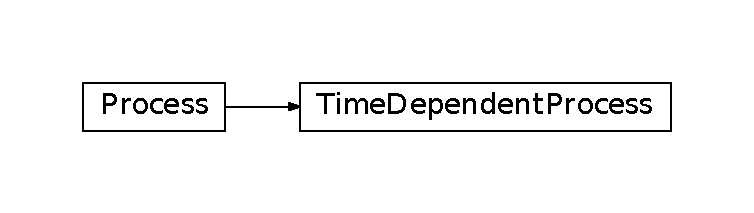
\includegraphics{inheritance-4aacab269f029f3f3453e58b89ba9679db78b256.pdf}
\phantomsection\label{api/climlab.process:module-climlab.process.time_dependent_process}\index{climlab.process.time\_dependent\_process (module)}\index{TimeDependentProcess (class in climlab.process.time\_dependent\_process)}

\begin{fulllineitems}
\phantomsection\label{api/climlab.process:climlab.process.time_dependent_process.TimeDependentProcess}\pysiglinewithargsret{\strong{class }\code{climlab.process.time\_dependent\_process.}\bfcode{TimeDependentProcess}}{\emph{time\_type='explicit'}, \emph{timestep=None}, \emph{topdown=True}, \emph{**kwargs}}{}
Bases: {\hyperref[api/climlab.process:climlab.process.process.Process]{\emph{\code{climlab.process.process.Process}}}} (\autopageref*{api/climlab.process:climlab.process.process.Process})

A generic parent class for all time-dependent processes.

\code{TimeDependentProcess} is a child of the 
{\hyperref[api/climlab.process:climlab.process.process.Process]{\emph{\code{Process}}}} (\autopageref*{api/climlab.process:climlab.process.process.Process}) class and therefore inherits
all those attributes.

\textbf{Initialization parameters}

An instance of \code{TimeDependentProcess} is initialized with the following 
arguments \emph{(for detailed information see Object attributes below)}:
\begin{quote}\begin{description}
\item[{Parameters}] \leavevmode\begin{itemize}
\item {} 
\textbf{\texttt{timestep}} (\href{http://docs.python.org/2.7/library/functions.html\#float}{\emph{\texttt{float}}}) -- specifies the timestep of the object (optional)

\item {} 
\textbf{\texttt{time\_type}} (\href{http://docs.python.org/2.7/library/functions.html\#str}{\emph{\texttt{str}}}) -- how time-dependent-process should be computed 
{[}default: `explicit'{]}

\item {} 
\textbf{\texttt{topdown}} (\href{http://docs.python.org/2.7/library/functions.html\#bool}{\emph{\texttt{bool}}}) -- whether geneterate \emph{process\_types} in regular or 
in reverse order {[}default: True{]}

\end{itemize}

\end{description}\end{quote}

\textbf{Object attributes}

Additional to the parent class {\hyperref[api/climlab.process:climlab.process.process.Process]{\emph{\code{Process}}}} (\autopageref*{api/climlab.process:climlab.process.process.Process})
following object attributes are generated during initialization:
\begin{quote}\begin{description}
\item[{Variables}] \leavevmode\begin{itemize}
\item {} 
\textbf{\texttt{has\_process\_type\_list}} (\href{http://docs.python.org/2.7/library/functions.html\#bool}{\emph{\texttt{bool}}}) -- information whether attribute \emph{process\_types} 
(which is needed for {\hyperref[api/climlab.process:climlab.process.time_dependent_process.TimeDependentProcess.compute]{\emph{\code{compute()}}}} (\autopageref*{api/climlab.process:climlab.process.time_dependent_process.TimeDependentProcess.compute}) and build in
\code{\_build\_process\_type\_list()})
exists or not. Attribute is set to \code{'False'} 
during initialization.

\item {} 
\textbf{\texttt{topdown}} (\href{http://docs.python.org/2.7/library/functions.html\#bool}{\emph{\texttt{bool}}}) -- information whether the list \emph{process\_types} (which 
contains all processes and sub-processes) should be 
generated in regular or in reverse order.
See \code{\_build\_process\_type\_list()}.

\item {} 
\textbf{\texttt{timeave}} (\href{http://docs.python.org/2.7/library/stdtypes.html\#dict}{\emph{\texttt{dict}}}) -- a time averaged collection of all states and diagnostic 
processes over the timeperiod that 
{\hyperref[api/climlab.process:climlab.process.time_dependent_process.TimeDependentProcess.integrate_years]{\emph{\code{integrate\_years()}}}} (\autopageref*{api/climlab.process:climlab.process.time_dependent_process.TimeDependentProcess.integrate_years}) has been called for last.

\item {} 
\textbf{\texttt{tendencies}} (\href{http://docs.python.org/2.7/library/stdtypes.html\#dict}{\emph{\texttt{dict}}}) -- computed difference in a timestep for each state. 
See {\hyperref[api/climlab.process:climlab.process.time_dependent_process.TimeDependentProcess.compute]{\emph{\code{compute()}}}} (\autopageref*{api/climlab.process:climlab.process.time_dependent_process.TimeDependentProcess.compute}) for details.

\item {} 
\textbf{\texttt{time\_type}} (\href{http://docs.python.org/2.7/library/functions.html\#str}{\emph{\texttt{str}}}) -- how time-dependent-process should be computed. 
Possible values are: \code{'explicit'}, \code{'implicit'},
\code{'diagnostic'}, \code{'adjustment'}.

\item {} 
\href{http://docs.python.org/2.7/library/time.html\#module-time}{\textbf{\texttt{time}}} (\href{http://docs.python.org/2.7/library/stdtypes.html\#dict}{\emph{\texttt{dict}}}) -- \begin{description}
\item[{a collection of all time-related attributes of the process. }] \leavevmode
The dictionary contains following items:

\end{description}
\begin{itemize}
\item {} 
\code{'timestep'}: see initialization parameter

\item {} 
\code{'num\_steps\_per\_year'}: see {\hyperref[api/climlab.process:climlab.process.time_dependent_process.TimeDependentProcess.set_timestep]{\emph{\code{set\_timestep()}}}} (\autopageref*{api/climlab.process:climlab.process.time_dependent_process.TimeDependentProcess.set_timestep}) and {\hyperref[api/climlab.process:climlab.process.time_dependent_process.TimeDependentProcess.timestep]{\emph{\code{timestep()}}}} (\autopageref*{api/climlab.process:climlab.process.time_dependent_process.TimeDependentProcess.timestep}) for details

\item {} 
\code{'day\_of\_year\_index'}: counter how many steps have been integrated in current year

\item {} 
\code{'steps'}: counter how many steps have been integrated in total

\item {} 
\code{'days\_elapsed'}: time counter for days

\item {} 
\code{'years\_elapsed'}: time counter for years

\item {} 
\code{'days\_of\_year'}: array which holds the number of numerical steps per year, expressed in days

\end{itemize}


\end{itemize}

\end{description}\end{quote}
\index{compute() (climlab.process.time\_dependent\_process.TimeDependentProcess method)}

\begin{fulllineitems}
\phantomsection\label{api/climlab.process:climlab.process.time_dependent_process.TimeDependentProcess.compute}\pysiglinewithargsret{\bfcode{compute}}{}{}
Computes the tendencies for all state variables given current state 
and specified input.

The function first computes all diagnostic processes. They don't produce 
any tendencies directly but they may effect the other processes (such as
change in solar distribution). Subsequently, all tendencies and 
diagnostics for all explicit processes are computed.

Tendencies due to implicit and adjustment processes need to be
calculated from a state that is already adjusted after explicit 
alteration. For that reason the explicit tendencies are applied to the 
states temporarily. Now all tendencies from implicit processes are 
calculated by matrix inversions and similar to the explicit tendencies,
the implicit ones are applied to the states temporarily. Subsequently,
all instantaneous adjustments are computed.

Then the changes that were made to the states from explicit and implicit 
processes are removed again as this 
{\hyperref[api/climlab.process:climlab.process.time_dependent_process.TimeDependentProcess.compute]{\emph{\code{compute()}}}} (\autopageref*{api/climlab.process:climlab.process.time_dependent_process.TimeDependentProcess.compute})
function is supposed to calculate only tendencies and not apply them 
to the states.

Finally, all calculated tendencies from all processes are collected 
for each state, summed up and stored in the dictionary 
\code{self.tendencies}, which is an attribute of the time-dependent-process 
object, for which the 
{\hyperref[api/climlab.process:climlab.process.time_dependent_process.TimeDependentProcess.compute]{\emph{\code{compute()}}}} (\autopageref*{api/climlab.process:climlab.process.time_dependent_process.TimeDependentProcess.compute})
method has been called.

\textbf{Object attributes}

During method execution following object attributes are modified:
\begin{quote}\begin{description}
\item[{Variables}] \leavevmode\begin{itemize}
\item {} 
\textbf{\texttt{tendencies}} (\href{http://docs.python.org/2.7/library/stdtypes.html\#dict}{\emph{\texttt{dict}}}) -- dictionary that holds tendencies for all states
is calculated for current timestep through 
adding up tendencies from explicit, implicit and
adjustment processes.

\item {} 
\textbf{\texttt{diagnostics}} (\href{http://docs.python.org/2.7/library/stdtypes.html\#dict}{\emph{\texttt{dict}}}) -- process diagnostic dictionary is updated 
by diagnostic dictionaries of subprocesses 
after computation of tendencies.

\end{itemize}

\end{description}\end{quote}

\end{fulllineitems}

\index{compute\_diagnostics() (climlab.process.time\_dependent\_process.TimeDependentProcess method)}

\begin{fulllineitems}
\phantomsection\label{api/climlab.process:climlab.process.time_dependent_process.TimeDependentProcess.compute_diagnostics}\pysiglinewithargsret{\bfcode{compute\_diagnostics}}{\emph{num\_iter=3}}{}
Compute all tendencies and diagnostics, but don't update model state.
By default it will call compute() 3 times to make sure all
subprocess coupling is accounted for. The number of iterations can
be changed with the input argument.

\end{fulllineitems}

\index{integrate\_converge() (climlab.process.time\_dependent\_process.TimeDependentProcess method)}

\begin{fulllineitems}
\phantomsection\label{api/climlab.process:climlab.process.time_dependent_process.TimeDependentProcess.integrate_converge}\pysiglinewithargsret{\bfcode{integrate\_converge}}{\emph{crit=0.0001}, \emph{verbose=True}}{}
Integrates the model until model states are converging.
\begin{quote}\begin{description}
\item[{Parameters}] \leavevmode\begin{itemize}
\item {} 
\textbf{\texttt{crit}} (\href{http://docs.python.org/2.7/library/functions.html\#float}{\emph{\texttt{float}}}) -- exit criteria for difference of iterated
solutions {[}default: 0.0001{]}

\item {} 
\textbf{\texttt{verbose}} (\href{http://docs.python.org/2.7/library/functions.html\#bool}{\emph{\texttt{bool}}}) -- information whether total elapsed time 
should be printed {[}default: True{]}

\end{itemize}

\item[{Example}] \leavevmode
\begin{Verbatim}[commandchars=\\\{\}]
\PYG{g+gp}{\PYGZgt{}\PYGZgt{}\PYGZgt{} }\PYG{k+kn}{import} \PYG{n+nn}{climlab}
\PYG{g+gp}{\PYGZgt{}\PYGZgt{}\PYGZgt{} }\PYG{n}{model} \PYG{o}{=} \PYG{n}{climlab}\PYG{o}{.}\PYG{n}{EBM}\PYG{p}{(}\PYG{p}{)}

\PYG{g+gp}{\PYGZgt{}\PYGZgt{}\PYGZgt{} }\PYG{n}{model}\PYG{o}{.}\PYG{n}{global\PYGZus{}mean\PYGZus{}temperature}\PYG{p}{(}\PYG{p}{)}
\PYG{g+go}{Field(11.997968598413685)}

\PYG{g+gp}{\PYGZgt{}\PYGZgt{}\PYGZgt{} }\PYG{n}{model}\PYG{o}{.}\PYG{n}{integrate\PYGZus{}converge}\PYG{p}{(}\PYG{p}{)}
\PYG{g+go}{Total elapsed time is 10.0 years.}

\PYG{g+gp}{\PYGZgt{}\PYGZgt{}\PYGZgt{} }\PYG{n}{model}\PYG{o}{.}\PYG{n}{global\PYGZus{}mean\PYGZus{}temperature}\PYG{p}{(}\PYG{p}{)}
\PYG{g+go}{Field(14.288155406577301)}
\end{Verbatim}

\end{description}\end{quote}

\end{fulllineitems}

\index{integrate\_days() (climlab.process.time\_dependent\_process.TimeDependentProcess method)}

\begin{fulllineitems}
\phantomsection\label{api/climlab.process:climlab.process.time_dependent_process.TimeDependentProcess.integrate_days}\pysiglinewithargsret{\bfcode{integrate\_days}}{\emph{days=1.0}, \emph{verbose=True}}{}
Integrates the model forward for a specified number of days.

It convertes the given number of days into years and calls 
{\hyperref[api/climlab.process:climlab.process.time_dependent_process.TimeDependentProcess.integrate_years]{\emph{\code{integrate\_years()}}}} (\autopageref*{api/climlab.process:climlab.process.time_dependent_process.TimeDependentProcess.integrate_years}).
\begin{quote}\begin{description}
\item[{Parameters}] \leavevmode\begin{itemize}
\item {} 
\textbf{\texttt{days}} (\href{http://docs.python.org/2.7/library/functions.html\#float}{\emph{\texttt{float}}}) -- integration time for the model in days      
{[}default: 1.0{]}

\item {} 
\textbf{\texttt{verbose}} (\href{http://docs.python.org/2.7/library/functions.html\#bool}{\emph{\texttt{bool}}}) -- information whether model time details 
should be printed {[}default: True{]}

\end{itemize}

\item[{Example}] \leavevmode
\begin{Verbatim}[commandchars=\\\{\}]
\PYG{g+gp}{\PYGZgt{}\PYGZgt{}\PYGZgt{} }\PYG{k+kn}{import} \PYG{n+nn}{climlab}
\PYG{g+gp}{\PYGZgt{}\PYGZgt{}\PYGZgt{} }\PYG{n}{model} \PYG{o}{=} \PYG{n}{climlab}\PYG{o}{.}\PYG{n}{EBM}\PYG{p}{(}\PYG{p}{)}

\PYG{g+gp}{\PYGZgt{}\PYGZgt{}\PYGZgt{} }\PYG{n}{model}\PYG{o}{.}\PYG{n}{global\PYGZus{}mean\PYGZus{}temperature}\PYG{p}{(}\PYG{p}{)}
\PYG{g+go}{Field(11.997968598413685)}

\PYG{g+gp}{\PYGZgt{}\PYGZgt{}\PYGZgt{} }\PYG{n}{model}\PYG{o}{.}\PYG{n}{integrate\PYGZus{}days}\PYG{p}{(}\PYG{l+m+mf}{80.}\PYG{p}{)}
\PYG{g+go}{Integrating for 19 steps, 80.0 days, or 0.219032740466 years.}
\PYG{g+go}{Total elapsed time is 0.211111111111 years.}
\PYG{g+go}{                }
\PYG{g+gp}{\PYGZgt{}\PYGZgt{}\PYGZgt{} }\PYG{n}{model}\PYG{o}{.}\PYG{n}{global\PYGZus{}mean\PYGZus{}temperature}\PYG{p}{(}\PYG{p}{)}
\PYG{g+go}{Field(11.873680783355553)}
\end{Verbatim}

\end{description}\end{quote}

\end{fulllineitems}

\index{integrate\_years() (climlab.process.time\_dependent\_process.TimeDependentProcess method)}

\begin{fulllineitems}
\phantomsection\label{api/climlab.process:climlab.process.time_dependent_process.TimeDependentProcess.integrate_years}\pysiglinewithargsret{\bfcode{integrate\_years}}{\emph{years=1.0}, \emph{verbose=True}}{}
Integrates the model by a given number of years.
\begin{quote}\begin{description}
\item[{Parameters}] \leavevmode\begin{itemize}
\item {} 
\textbf{\texttt{years}} (\href{http://docs.python.org/2.7/library/functions.html\#float}{\emph{\texttt{float}}}) -- integration time for the model in years     
{[}default: 1.0{]}

\item {} 
\textbf{\texttt{verbose}} (\href{http://docs.python.org/2.7/library/functions.html\#bool}{\emph{\texttt{bool}}}) -- information whether model time details 
should be printed {[}default: True{]}

\end{itemize}

\end{description}\end{quote}

It calls {\hyperref[api/climlab.process:climlab.process.time_dependent_process.TimeDependentProcess.step_forward]{\emph{\code{step\_forward()}}}} (\autopageref*{api/climlab.process:climlab.process.time_dependent_process.TimeDependentProcess.step_forward}) repetitively and calculates a time 
averaged value over the integrated period for every model state and all
diagnostics processes.
\begin{quote}\begin{description}
\item[{Example}] \leavevmode
\begin{Verbatim}[commandchars=\\\{\}]
\PYG{g+gp}{\PYGZgt{}\PYGZgt{}\PYGZgt{} }\PYG{k+kn}{import} \PYG{n+nn}{climlab}
\PYG{g+gp}{\PYGZgt{}\PYGZgt{}\PYGZgt{} }\PYG{n}{model} \PYG{o}{=} \PYG{n}{climlab}\PYG{o}{.}\PYG{n}{EBM}\PYG{p}{(}\PYG{p}{)}

\PYG{g+gp}{\PYGZgt{}\PYGZgt{}\PYGZgt{} }\PYG{n}{model}\PYG{o}{.}\PYG{n}{global\PYGZus{}mean\PYGZus{}temperature}\PYG{p}{(}\PYG{p}{)}
\PYG{g+go}{Field(11.997968598413685)}

\PYG{g+gp}{\PYGZgt{}\PYGZgt{}\PYGZgt{} }\PYG{n}{model}\PYG{o}{.}\PYG{n}{integrate\PYGZus{}years}\PYG{p}{(}\PYG{l+m+mf}{2.}\PYG{p}{)}
\PYG{g+go}{Integrating for 180 steps, 730.4844 days, or 2.0 years.}
\PYG{g+go}{Total elapsed time is 2.0 years.}
\PYG{g+go}{                                }
\PYG{g+gp}{\PYGZgt{}\PYGZgt{}\PYGZgt{} }\PYG{n}{model}\PYG{o}{.}\PYG{n}{global\PYGZus{}mean\PYGZus{}temperature}\PYG{p}{(}\PYG{p}{)}
\PYG{g+go}{Field(13.531055349437258)}
\end{Verbatim}

\end{description}\end{quote}

\end{fulllineitems}

\index{set\_timestep() (climlab.process.time\_dependent\_process.TimeDependentProcess method)}

\begin{fulllineitems}
\phantomsection\label{api/climlab.process:climlab.process.time_dependent_process.TimeDependentProcess.set_timestep}\pysiglinewithargsret{\bfcode{set\_timestep}}{\emph{timestep=86400.0}, \emph{num\_steps\_per\_year=None}}{}
Calculates the timestep in unit seconds
and calls the setter function of {\hyperref[api/climlab.process:climlab.process.time_dependent_process.TimeDependentProcess.timestep]{\emph{\code{timestep()}}}} (\autopageref*{api/climlab.process:climlab.process.time_dependent_process.TimeDependentProcess.timestep})
\begin{quote}\begin{description}
\item[{Parameters}] \leavevmode\begin{itemize}
\item {} 
\textbf{\texttt{timestep}} (\href{http://docs.python.org/2.7/library/functions.html\#float}{\emph{\texttt{float}}}) -- the amount of time over which 
{\hyperref[api/climlab.process:climlab.process.time_dependent_process.TimeDependentProcess.step_forward]{\emph{\code{step\_forward()}}}} (\autopageref*{api/climlab.process:climlab.process.time_dependent_process.TimeDependentProcess.step_forward}) is integrating 
in unit seconds {[}default: 24*60*60{]}

\item {} 
\textbf{\texttt{num\_steps\_per\_year}} (\href{http://docs.python.org/2.7/library/functions.html\#float}{\emph{\texttt{float}}}) -- a number of steps per calendar year 
(optional)

\end{itemize}

\end{description}\end{quote}

If the parameter \emph{num\_steps\_per\_year} is specified and not \code{None}, 
the timestep is calculated accordingly and therefore the given input
parameter \emph{timestep} is ignored.

\end{fulllineitems}

\index{step\_forward() (climlab.process.time\_dependent\_process.TimeDependentProcess method)}

\begin{fulllineitems}
\phantomsection\label{api/climlab.process:climlab.process.time_dependent_process.TimeDependentProcess.step_forward}\pysiglinewithargsret{\bfcode{step\_forward}}{}{}
Updates state variables with computed tendencies.

Calls the {\hyperref[api/climlab.process:climlab.process.time_dependent_process.TimeDependentProcess.compute]{\emph{\code{compute()}}}} (\autopageref*{api/climlab.process:climlab.process.time_dependent_process.TimeDependentProcess.compute}) method to get current tendencies for all
process states. Multiplied with the timestep and added up to the state
variables is updating all model states.
\begin{quote}\begin{description}
\item[{Example}] \leavevmode
\begin{Verbatim}[commandchars=\\\{\}]
\PYG{g+gp}{\PYGZgt{}\PYGZgt{}\PYGZgt{} }\PYG{k+kn}{import} \PYG{n+nn}{climlab}
\PYG{g+gp}{\PYGZgt{}\PYGZgt{}\PYGZgt{} }\PYG{n}{model} \PYG{o}{=} \PYG{n}{climlab}\PYG{o}{.}\PYG{n}{EBM}\PYG{p}{(}\PYG{p}{)}

\PYG{g+gp}{\PYGZgt{}\PYGZgt{}\PYGZgt{} }\PYG{c+c1}{\PYGZsh{} checking time step counter}
\PYG{g+gp}{\PYGZgt{}\PYGZgt{}\PYGZgt{} }\PYG{n}{model}\PYG{o}{.}\PYG{n}{time}\PYG{p}{[}\PYG{l+s+s1}{\PYGZsq{}}\PYG{l+s+s1}{steps}\PYG{l+s+s1}{\PYGZsq{}}\PYG{p}{]}
\PYG{g+go}{0}

\PYG{g+gp}{\PYGZgt{}\PYGZgt{}\PYGZgt{} }\PYG{c+c1}{\PYGZsh{} stepping the model forward}
\PYG{g+gp}{\PYGZgt{}\PYGZgt{}\PYGZgt{} }\PYG{n}{model}\PYG{o}{.}\PYG{n}{step\PYGZus{}forward}\PYG{p}{(}\PYG{p}{)}

\PYG{g+gp}{\PYGZgt{}\PYGZgt{}\PYGZgt{} }\PYG{c+c1}{\PYGZsh{} step counter increased}
\PYG{g+gp}{\PYGZgt{}\PYGZgt{}\PYGZgt{} }\PYG{n}{model}\PYG{o}{.}\PYG{n}{time}\PYG{p}{[}\PYG{l+s+s1}{\PYGZsq{}}\PYG{l+s+s1}{steps}\PYG{l+s+s1}{\PYGZsq{}}\PYG{p}{]}
\PYG{g+go}{1}
\end{Verbatim}

\end{description}\end{quote}

\end{fulllineitems}

\index{timestep (climlab.process.time\_dependent\_process.TimeDependentProcess attribute)}

\begin{fulllineitems}
\phantomsection\label{api/climlab.process:climlab.process.time_dependent_process.TimeDependentProcess.timestep}\pysigline{\bfcode{timestep}}
The amount of time over which {\hyperref[api/climlab.process:climlab.process.time_dependent_process.TimeDependentProcess.step_forward]{\emph{\code{step\_forward()}}}} (\autopageref*{api/climlab.process:climlab.process.time_dependent_process.TimeDependentProcess.step_forward}) is integrating in unit seconds.
\begin{quote}\begin{description}
\item[{Getter}] \leavevmode
Returns the object timestep which is stored in \code{self.param{[}'timestep'{]}}.

\item[{Setter}] \leavevmode
Sets the timestep to the given input. See also {\hyperref[api/climlab.process:climlab.process.time_dependent_process.TimeDependentProcess.set_timestep]{\emph{\code{set\_timestep()}}}} (\autopageref*{api/climlab.process:climlab.process.time_dependent_process.TimeDependentProcess.set_timestep}).

\item[{Type}] \leavevmode
float

\end{description}\end{quote}

\end{fulllineitems}


\end{fulllineitems}



\subsection{climlab.radiation package}
\label{api/climlab.radiation:climlab-radiation-package}\label{api/climlab.radiation::doc}

\subsubsection{climlab.radiation.AplusBT module}
\label{api/climlab.radiation:climlab-radiation-aplusbt-module}
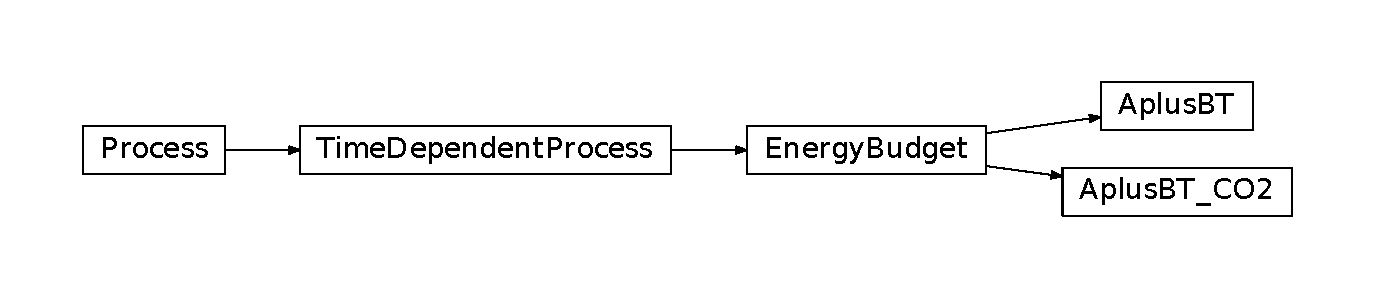
\includegraphics{inheritance-02be59372c5ce161a2b728197b304d7b4804f2e1.pdf}
\phantomsection\label{api/climlab.radiation:module-climlab.radiation.AplusBT}\index{climlab.radiation.AplusBT (module)}\index{AplusBT (class in climlab.radiation.AplusBT)}

\begin{fulllineitems}
\phantomsection\label{api/climlab.radiation:climlab.radiation.AplusBT.AplusBT}\pysiglinewithargsret{\strong{class }\code{climlab.radiation.AplusBT.}\bfcode{AplusBT}}{\emph{A=200.0}, \emph{B=2.0}, \emph{**kwargs}}{}
Bases: {\hyperref[api/climlab.process:climlab.process.energy_budget.EnergyBudget]{\emph{\code{climlab.process.energy\_budget.EnergyBudget}}}} (\autopageref*{api/climlab.process:climlab.process.energy_budget.EnergyBudget})

The simplest linear longwave radiation module.

Calculates the Outgoing Longwave Radation (OLR) \(R\uparrow\) as
\begin{gather}
\begin{split}R\uparrow = A + B \cdot T\end{split}\notag
\end{gather}
where \(T\) is the state variable.

Should be invoked with a single temperature state variable only.

\textbf{Initialization parameters}

An instance of \code{AplusBT} is initialized with the following 
arguments:
\begin{quote}\begin{description}
\item[{Parameters}] \leavevmode\begin{itemize}
\item {} 
\textbf{\texttt{A}} (\href{http://docs.python.org/2.7/library/functions.html\#float}{\emph{\texttt{float}}}) -- 
parameter for linear OLR parametrization
\begin{itemize}
\item {} 
unit: \(\frac{\textrm{W}}
{\textrm{m}^2}\)

\item {} 
default value: \code{200.0}

\end{itemize}


\item {} 
\textbf{\texttt{B}} (\href{http://docs.python.org/2.7/library/functions.html\#float}{\emph{\texttt{float}}}) -- 
parameter for linear OLR parametrization
\begin{itemize}
\item {} 
unit: \(\frac{\textrm{W}}
{\textrm{m}^2 \ ^{\circ} \textrm{C}}\)

\item {} 
default value: \code{2.0}

\end{itemize}


\end{itemize}

\end{description}\end{quote}

\textbf{Object attributes}

Additional to the parent class {\hyperref[api/climlab.process:climlab.process.energy_budget.EnergyBudget]{\emph{\code{EnergyBudget}}}} (\autopageref*{api/climlab.process:climlab.process.energy_budget.EnergyBudget})
following object attributes are generated or modified during initialization:
\begin{quote}\begin{description}
\item[{Variables}] \leavevmode\begin{itemize}
\item {} 
{\hyperref[api/climlab.radiation:climlab.radiation.AplusBT.AplusBT.A]{\emph{\textbf{\texttt{A}}}}} (\autopageref*{api/climlab.radiation:climlab.radiation.AplusBT.AplusBT.A}) (\href{http://docs.python.org/2.7/library/functions.html\#float}{\emph{\texttt{float}}}) -- calls the setter function of {\hyperref[api/climlab.radiation:climlab.radiation.AplusBT.AplusBT.A]{\emph{\code{A()}}}} (\autopageref*{api/climlab.radiation:climlab.radiation.AplusBT.AplusBT.A})

\item {} 
{\hyperref[api/climlab.radiation:climlab.radiation.AplusBT.AplusBT.B]{\emph{\textbf{\texttt{B}}}}} (\autopageref*{api/climlab.radiation:climlab.radiation.AplusBT.AplusBT.B}) (\href{http://docs.python.org/2.7/library/functions.html\#float}{\emph{\texttt{float}}}) -- calls the setter function of {\hyperref[api/climlab.radiation:climlab.radiation.AplusBT.AplusBT.B]{\emph{\code{B()}}}} (\autopageref*{api/climlab.radiation:climlab.radiation.AplusBT.AplusBT.B})

\item {} 
\textbf{\texttt{diagnostics}} (\href{http://docs.python.org/2.7/library/stdtypes.html\#dict}{\emph{\texttt{dict}}}) -- key \code{'OLR'} initialized with value:
{\hyperref[api/climlab.domain:climlab.domain.field.Field]{\emph{\code{Field}}}} (\autopageref*{api/climlab.domain:climlab.domain.field.Field}) of zeros
in size of \code{self.Ts}

\item {} 
{\hyperref[api/climlab.radiation:climlab.radiation.AplusBT.AplusBT.OLR]{\emph{\textbf{\texttt{OLR}}}}} (\autopageref*{api/climlab.radiation:climlab.radiation.AplusBT.AplusBT.OLR}) ({\hyperref[api/climlab.domain:climlab.domain.field.Field]{\emph{\emph{\texttt{Field}}}}} (\autopageref*{api/climlab.domain:climlab.domain.field.Field})) -- the subprocess attribute \code{self.OLR} is
created with correct dimensions

\end{itemize}

\end{description}\end{quote}

\begin{notice}{warning}{Warning:}
This module currently works only for a single state variable!
\end{notice}
\begin{quote}\begin{description}
\item[{Example}] \leavevmode
Simple linear radiation module (stand alone):

\begin{Verbatim}[commandchars=\\\{\}]
\PYG{g+gp}{\PYGZgt{}\PYGZgt{}\PYGZgt{} }\PYG{k+kn}{import} \PYG{n+nn}{climlab}

\PYG{g+gp}{\PYGZgt{}\PYGZgt{}\PYGZgt{} }\PYG{c+c1}{\PYGZsh{} create a column atmosphere and scalar surface}
\PYG{g+gp}{\PYGZgt{}\PYGZgt{}\PYGZgt{} }\PYG{n}{sfc}\PYG{p}{,} \PYG{n}{atm} \PYG{o}{=} \PYG{n}{climlab}\PYG{o}{.}\PYG{n}{domain}\PYG{o}{.}\PYG{n}{single\PYGZus{}column}\PYG{p}{(}\PYG{p}{)}  

\PYG{g+gp}{\PYGZgt{}\PYGZgt{}\PYGZgt{} }\PYG{c+c1}{\PYGZsh{} Create a state variable}
\PYG{g+gp}{\PYGZgt{}\PYGZgt{}\PYGZgt{} }\PYG{n}{Ts} \PYG{o}{=} \PYG{n}{climlab}\PYG{o}{.}\PYG{n}{Field}\PYG{p}{(}\PYG{l+m+mf}{15.}\PYG{p}{,} \PYG{n}{domain}\PYG{o}{=}\PYG{n}{sfc}\PYG{p}{)}

\PYG{g+gp}{\PYGZgt{}\PYGZgt{}\PYGZgt{} }\PYG{c+c1}{\PYGZsh{} Make a dictionary of state variables}
\PYG{g+gp}{\PYGZgt{}\PYGZgt{}\PYGZgt{} }\PYG{n}{s} \PYG{o}{=} \PYG{p}{\PYGZob{}}\PYG{l+s+s1}{\PYGZsq{}}\PYG{l+s+s1}{Ts}\PYG{l+s+s1}{\PYGZsq{}}\PYG{p}{:} \PYG{n}{Ts}\PYG{p}{\PYGZcb{}}

\PYG{g+gp}{\PYGZgt{}\PYGZgt{}\PYGZgt{} }\PYG{c+c1}{\PYGZsh{} create process}
\PYG{g+gp}{\PYGZgt{}\PYGZgt{}\PYGZgt{} }\PYG{n}{olr} \PYG{o}{=} \PYG{n}{climlab}\PYG{o}{.}\PYG{n}{radiation}\PYG{o}{.}\PYG{n}{AplusBT}\PYG{p}{(}\PYG{n}{state}\PYG{o}{=}\PYG{n}{s}\PYG{p}{)}

\PYG{g+gp}{\PYGZgt{}\PYGZgt{}\PYGZgt{} }\PYG{k}{print} \PYG{n}{olr}
\PYG{g+go}{climlab Process of type \PYGZlt{}class \PYGZsq{}climlab.radiation.AplusBT.AplusBT\PYGZsq{}\PYGZgt{}. }
\PYG{g+go}{State variables and domain shapes: }
\PYG{g+go}{  Ts: (1,) }
\PYG{g+go}{The subprocess tree: }
\PYG{g+go}{top: \PYGZlt{}class \PYGZsq{}climlab.radiation.AplusBT.AplusBT\PYGZsq{}\PYGZgt{}}

\PYG{g+gp}{\PYGZgt{}\PYGZgt{}\PYGZgt{} }\PYG{c+c1}{\PYGZsh{} to compute tendencies and diagnostics}
\PYG{g+gp}{\PYGZgt{}\PYGZgt{}\PYGZgt{} }\PYG{n}{olr}\PYG{o}{.}\PYG{n}{compute}\PYG{p}{(}\PYG{p}{)}

\PYG{g+gp}{\PYGZgt{}\PYGZgt{}\PYGZgt{} }\PYG{c+c1}{\PYGZsh{}  or to actually update the temperature}
\PYG{g+gp}{\PYGZgt{}\PYGZgt{}\PYGZgt{} }\PYG{n}{olr}\PYG{o}{.}\PYG{n}{step\PYGZus{}forward}\PYG{p}{(}\PYG{p}{)}

\PYG{g+gp}{\PYGZgt{}\PYGZgt{}\PYGZgt{} }\PYG{k}{print} \PYG{n}{olr}\PYG{o}{.}\PYG{n}{state}
\PYG{g+go}{\PYGZob{}\PYGZsq{}Ts\PYGZsq{}: Field([ 5.69123176])\PYGZcb{}}
\end{Verbatim}

\end{description}\end{quote}
\index{A (climlab.radiation.AplusBT.AplusBT attribute)}

\begin{fulllineitems}
\phantomsection\label{api/climlab.radiation:climlab.radiation.AplusBT.AplusBT.A}\pysigline{\bfcode{A}}
Property of AplusBT parameter A.
\begin{quote}\begin{description}
\item[{Getter}] \leavevmode
Returns the parameter A which is stored in attribute 
\code{self.\_A}

\item[{Setter}] \leavevmode\begin{itemize}
\item {} 
sets parameter A which is addressed as \code{self.\_A}
to the new value

\item {} 
updates the parameter dictionary \code{self.param{[}'A'{]}}

\end{itemize}

\item[{Type}] \leavevmode
float

\item[{Example}] \leavevmode
\begin{Verbatim}[commandchars=\\\{\}]
\PYG{g+gp}{\PYGZgt{}\PYGZgt{}\PYGZgt{} }\PYG{k+kn}{import} \PYG{n+nn}{climlab}
\PYG{g+gp}{\PYGZgt{}\PYGZgt{}\PYGZgt{} }\PYG{n}{model} \PYG{o}{=} \PYG{n}{climlab}\PYG{o}{.}\PYG{n}{EBM}\PYG{p}{(}\PYG{p}{)}

\PYG{g+gp}{\PYGZgt{}\PYGZgt{}\PYGZgt{} }\PYG{c+c1}{\PYGZsh{} getter}
\PYG{g+gp}{\PYGZgt{}\PYGZgt{}\PYGZgt{} }\PYG{n}{model}\PYG{o}{.}\PYG{n}{subprocess}\PYG{p}{[}\PYG{l+s+s1}{\PYGZsq{}}\PYG{l+s+s1}{LW}\PYG{l+s+s1}{\PYGZsq{}}\PYG{p}{]}\PYG{o}{.}\PYG{n}{A}
\PYG{g+go}{210.0}
\PYG{g+gp}{\PYGZgt{}\PYGZgt{}\PYGZgt{} }\PYG{c+c1}{\PYGZsh{} setter}
\PYG{g+gp}{\PYGZgt{}\PYGZgt{}\PYGZgt{} }\PYG{n}{model}\PYG{o}{.}\PYG{n}{subprocess}\PYG{p}{[}\PYG{l+s+s1}{\PYGZsq{}}\PYG{l+s+s1}{LW}\PYG{l+s+s1}{\PYGZsq{}}\PYG{p}{]}\PYG{o}{.}\PYG{n}{A} \PYG{o}{=} \PYG{l+m+mi}{220}
\PYG{g+gp}{\PYGZgt{}\PYGZgt{}\PYGZgt{} }\PYG{c+c1}{\PYGZsh{} getter again                }
\PYG{g+gp}{\PYGZgt{}\PYGZgt{}\PYGZgt{} }\PYG{n}{model}\PYG{o}{.}\PYG{n}{subprocess}\PYG{p}{[}\PYG{l+s+s1}{\PYGZsq{}}\PYG{l+s+s1}{LW}\PYG{l+s+s1}{\PYGZsq{}}\PYG{p}{]}\PYG{o}{.}\PYG{n}{A}
\PYG{g+go}{220}

\PYG{g+gp}{\PYGZgt{}\PYGZgt{}\PYGZgt{} }\PYG{c+c1}{\PYGZsh{} subprocess parameter dictionary}
\PYG{g+gp}{\PYGZgt{}\PYGZgt{}\PYGZgt{} }\PYG{n}{model}\PYG{o}{.}\PYG{n}{subprocess}\PYG{p}{[}\PYG{l+s+s1}{\PYGZsq{}}\PYG{l+s+s1}{LW}\PYG{l+s+s1}{\PYGZsq{}}\PYG{p}{]}\PYG{o}{.}\PYG{n}{param}\PYG{p}{[}\PYG{l+s+s1}{\PYGZsq{}}\PYG{l+s+s1}{A}\PYG{l+s+s1}{\PYGZsq{}}\PYG{p}{]}
\PYG{g+go}{220}
\end{Verbatim}

\end{description}\end{quote}

\end{fulllineitems}

\index{B (climlab.radiation.AplusBT.AplusBT attribute)}

\begin{fulllineitems}
\phantomsection\label{api/climlab.radiation:climlab.radiation.AplusBT.AplusBT.B}\pysigline{\bfcode{B}}
Property of AplusBT parameter B.
\begin{quote}\begin{description}
\item[{Getter}] \leavevmode
Returns the parameter B which is stored in attribute 
\code{self.\_B}

\item[{Setter}] \leavevmode\begin{itemize}
\item {} 
sets parameter B which is addressed as \code{self.\_B}
to the new value

\item {} 
updates the parameter dictionary \code{self.param{[}'B'{]}}

\end{itemize}

\item[{Type}] \leavevmode
float

\end{description}\end{quote}

\end{fulllineitems}

\index{OLR (climlab.radiation.AplusBT.AplusBT attribute)}

\begin{fulllineitems}
\phantomsection\label{api/climlab.radiation:climlab.radiation.AplusBT.AplusBT.OLR}\pysigline{\bfcode{OLR}}
\end{fulllineitems}


\end{fulllineitems}

\index{AplusBT\_CO2 (class in climlab.radiation.AplusBT)}

\begin{fulllineitems}
\phantomsection\label{api/climlab.radiation:climlab.radiation.AplusBT.AplusBT_CO2}\pysiglinewithargsret{\strong{class }\code{climlab.radiation.AplusBT.}\bfcode{AplusBT\_CO2}}{\emph{CO2=300.0}, \emph{**kwargs}}{}
Bases: {\hyperref[api/climlab.process:climlab.process.energy_budget.EnergyBudget]{\emph{\code{climlab.process.energy\_budget.EnergyBudget}}}} (\autopageref*{api/climlab.process:climlab.process.energy_budget.EnergyBudget})

Linear longwave radiation module considering CO2 concentration.

This radiation subprocess is based in the idea to linearize the Outgoing 
Longwave Radiation (OLR) emitted to space according to the surface temperature
(see {\hyperref[api/climlab.radiation:climlab.radiation.AplusBT.AplusBT]{\emph{\code{AplusBT}}}} (\autopageref*{api/climlab.radiation:climlab.radiation.AplusBT.AplusBT})).

To consider a the change of the greenhouse effect through range of
\(CO_2\) in the atmosphere, the parameters A and B are computed like
the following:
\begin{gather}
\begin{split}A(c) = -326.4 + 9.161 c - 3.164 c^2 + 0.5468 c^3            \end{split}\notag\\\begin{split}B(c) =  1.953 - 0.04866 c + 0.01309 c^2 - 0.002577 c^3\end{split}\notag
\end{gather}
where \(c=\log \frac{p}{300}\) and \(p\) represents 
the concentration of \(CO_2\) in the atmosphere.

For further reading see {[}Caldeira\_1992{]}.

\textbf{Initialization parameters}

An instance of \code{AplusBT\_CO2} is initialized with the following 
argument:
\begin{quote}\begin{description}
\item[{Parameters}] \leavevmode
\textbf{\texttt{CO2}} (\href{http://docs.python.org/2.7/library/functions.html\#float}{\emph{\texttt{float}}}) -- 
The concentration of \(CO_2\) in the atmosphere.
Referred to as \(p\) in the above given formulas.
\begin{itemize}
\item {} 
unit: \(\textrm{ppm}\) (parts per million)

\item {} 
default value: \code{300.0}

\end{itemize}


\end{description}\end{quote}

\textbf{Object attributes}

Additional to the parent class {\hyperref[api/climlab.process:climlab.process.energy_budget.EnergyBudget]{\emph{\code{EnergyBudget}}}} (\autopageref*{api/climlab.process:climlab.process.energy_budget.EnergyBudget})
following object attributes are generated or updated during initialization:
\begin{quote}\begin{description}
\item[{Variables}] \leavevmode\begin{itemize}
\item {} 
{\hyperref[api/climlab.radiation:climlab.radiation.AplusBT.AplusBT_CO2.CO2]{\emph{\textbf{\texttt{CO2}}}}} (\autopageref*{api/climlab.radiation:climlab.radiation.AplusBT.AplusBT_CO2.CO2}) (\href{http://docs.python.org/2.7/library/functions.html\#float}{\emph{\texttt{float}}}) -- calls the setter function of {\hyperref[api/climlab.radiation:climlab.radiation.AplusBT.AplusBT_CO2.CO2]{\emph{\code{CO2()}}}} (\autopageref*{api/climlab.radiation:climlab.radiation.AplusBT.AplusBT_CO2.CO2})

\item {} 
\textbf{\texttt{diagnostics}} (\href{http://docs.python.org/2.7/library/stdtypes.html\#dict}{\emph{\texttt{dict}}}) -- the subprocess's diagnostic dictionary 
\code{self.diagnostic} is initialized 
through calling 
\code{self.init\_diagnostic('OLR', 0. * self.Ts)}

\item {} 
{\hyperref[api/climlab.radiation:climlab.radiation.AplusBT.AplusBT.OLR]{\emph{\textbf{\texttt{OLR}}}}} (\autopageref*{api/climlab.radiation:climlab.radiation.AplusBT.AplusBT.OLR}) ({\hyperref[api/climlab.domain:climlab.domain.field.Field]{\emph{\emph{\texttt{Field}}}}} (\autopageref*{api/climlab.domain:climlab.domain.field.Field})) -- the subprocess attribute \code{self.OLR} is
created with correct dimensions

\end{itemize}

\item[{Example}] \leavevmode
Replacing an the regular AplusBT subprocess in an energy balance model:

\begin{Verbatim}[commandchars=\\\{\}]
\PYG{g+gp}{\PYGZgt{}\PYGZgt{}\PYGZgt{} }\PYG{k+kn}{import} \PYG{n+nn}{climlab}
\PYG{g+gp}{\PYGZgt{}\PYGZgt{}\PYGZgt{} }\PYG{k+kn}{from} \PYG{n+nn}{climlab.radiation.AplusBT} \PYG{k+kn}{import} \PYG{n}{AplusBT\PYGZus{}CO2}

\PYG{g+gp}{\PYGZgt{}\PYGZgt{}\PYGZgt{} }\PYG{c+c1}{\PYGZsh{} creating EBM model}
\PYG{g+gp}{\PYGZgt{}\PYGZgt{}\PYGZgt{} }\PYG{n}{model} \PYG{o}{=} \PYG{n}{climlab}\PYG{o}{.}\PYG{n}{EBM}\PYG{p}{(}\PYG{p}{)}
\PYG{g+go}{            }
\PYG{g+gp}{\PYGZgt{}\PYGZgt{}\PYGZgt{} }\PYG{k}{print} \PYG{n}{model}
\end{Verbatim}

\begin{Verbatim}[commandchars=\\\{\}]
climlab Process of type \PYGZlt{}class \PYGZsq{}climlab.model.ebm.EBM\PYGZsq{}\PYGZgt{}. 
State variables and domain shapes: 
  Ts: (90, 1) 
The subprocess tree: 
top: \PYGZlt{}class \PYGZsq{}climlab.model.ebm.EBM\PYGZsq{}\PYGZgt{}
   diffusion: \PYGZlt{}class \PYGZsq{}climlab.dynamics.diffusion.MeridionalDiffusion\PYGZsq{}\PYGZgt{}
   LW: \PYGZlt{}class \PYGZsq{}climlab.radiation.AplusBT.AplusBT\PYGZsq{}\PYGZgt{}
   albedo: \PYGZlt{}class \PYGZsq{}climlab.surface.albedo.StepFunctionAlbedo\PYGZsq{}\PYGZgt{}
      iceline: \PYGZlt{}class \PYGZsq{}climlab.surface.albedo.Iceline\PYGZsq{}\PYGZgt{}
      cold\PYGZus{}albedo: \PYGZlt{}class \PYGZsq{}climlab.surface.albedo.ConstantAlbedo\PYGZsq{}\PYGZgt{}
      warm\PYGZus{}albedo: \PYGZlt{}class \PYGZsq{}climlab.surface.albedo.P2Albedo\PYGZsq{}\PYGZgt{}
   insolation: \PYGZlt{}class \PYGZsq{}climlab.radiation.insolation.P2Insolation\PYGZsq{}\PYGZgt{}
\end{Verbatim}

\begin{Verbatim}[commandchars=\\\{\}]
\PYG{g+gp}{\PYGZgt{}\PYGZgt{}\PYGZgt{} }\PYG{c+c1}{\PYGZsh{}  creating and adding albedo feedback subprocess}
\PYG{g+gp}{\PYGZgt{}\PYGZgt{}\PYGZgt{} }\PYG{n}{LW\PYGZus{}CO2} \PYG{o}{=} \PYG{n}{AplusBT\PYGZus{}CO2}\PYG{p}{(}\PYG{n}{CO2}\PYG{o}{=}\PYG{l+m+mi}{400}\PYG{p}{,} \PYG{n}{state}\PYG{o}{=}\PYG{n}{model}\PYG{o}{.}\PYG{n}{state}\PYG{p}{,} \PYG{o}{*}\PYG{o}{*}\PYG{n}{model}\PYG{o}{.}\PYG{n}{param}\PYG{p}{)}

\PYG{g+gp}{\PYGZgt{}\PYGZgt{}\PYGZgt{} }\PYG{c+c1}{\PYGZsh{} overwriting old \PYGZsq{}LW\PYGZsq{} subprocess with same name  }
\PYG{g+gp}{\PYGZgt{}\PYGZgt{}\PYGZgt{} }\PYG{n}{model}\PYG{o}{.}\PYG{n}{add\PYGZus{}subprocess}\PYG{p}{(}\PYG{l+s+s1}{\PYGZsq{}}\PYG{l+s+s1}{LW}\PYG{l+s+s1}{\PYGZsq{}}\PYG{p}{,} \PYG{n}{LW\PYGZus{}CO2}\PYG{p}{)}

\PYG{g+gp}{\PYGZgt{}\PYGZgt{}\PYGZgt{} }\PYG{k}{print} \PYG{n}{model}
\end{Verbatim}

\begin{Verbatim}[commandchars=\\\{\}]
climlab Process of type \PYGZlt{}class \PYGZsq{}climlab.model.ebm.EBM\PYGZsq{}\PYGZgt{}. 
State variables and domain shapes: 
  Ts: (90, 1) 
The subprocess tree: 
top: \PYGZlt{}class \PYGZsq{}climlab.model.ebm.EBM\PYGZsq{}\PYGZgt{}
   diffusion: \PYGZlt{}class \PYGZsq{}climlab.dynamics.diffusion.MeridionalDiffusion\PYGZsq{}\PYGZgt{}
   LW: \PYGZlt{}class \PYGZsq{}climlab.radiation.AplusBT.AplusBT\PYGZus{}CO2\PYGZsq{}\PYGZgt{}
   albedo: \PYGZlt{}class \PYGZsq{}climlab.surface.albedo.StepFunctionAlbedo\PYGZsq{}\PYGZgt{}
      iceline: \PYGZlt{}class \PYGZsq{}climlab.surface.albedo.Iceline\PYGZsq{}\PYGZgt{}
      cold\PYGZus{}albedo: \PYGZlt{}class \PYGZsq{}climlab.surface.albedo.ConstantAlbedo\PYGZsq{}\PYGZgt{}
      warm\PYGZus{}albedo: \PYGZlt{}class \PYGZsq{}climlab.surface.albedo.P2Albedo\PYGZsq{}\PYGZgt{}
   insolation: \PYGZlt{}class \PYGZsq{}climlab.radiation.insolation.P2Insolation\PYGZsq{}\PYGZgt{}
\end{Verbatim}

\end{description}\end{quote}
\index{CO2 (climlab.radiation.AplusBT.AplusBT\_CO2 attribute)}

\begin{fulllineitems}
\phantomsection\label{api/climlab.radiation:climlab.radiation.AplusBT.AplusBT_CO2.CO2}\pysigline{\bfcode{CO2}}
Property of AplusBT\_CO2 parameter CO2.
\begin{quote}\begin{description}
\item[{Getter}] \leavevmode
Returns the CO2 concentration which is stored in attribute 
\code{self.\_CO2}

\item[{Setter}] \leavevmode\begin{itemize}
\item {} 
sets the CO2 concentration which is addressed as \code{self.\_CO2}
to the new value

\item {} 
updates the parameter dictionary \code{self.param{[}'CO2'{]}}

\end{itemize}

\item[{Type}] \leavevmode
float

\end{description}\end{quote}

\end{fulllineitems}


\end{fulllineitems}



\subsubsection{climlab.radiation.Boltzmann module}
\label{api/climlab.radiation:climlab-radiation-boltzmann-module}
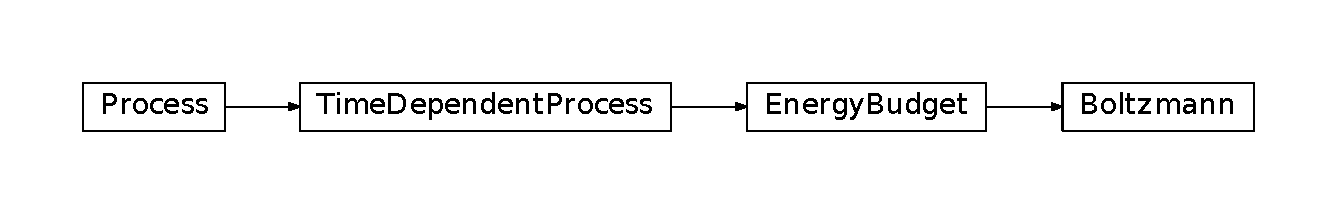
\includegraphics{inheritance-658ce4f2d58cd543b03b338809a90b211995f932.pdf}
\phantomsection\label{api/climlab.radiation:module-climlab.radiation.Boltzmann}\index{climlab.radiation.Boltzmann (module)}\index{Boltzmann (class in climlab.radiation.Boltzmann)}

\begin{fulllineitems}
\phantomsection\label{api/climlab.radiation:climlab.radiation.Boltzmann.Boltzmann}\pysiglinewithargsret{\strong{class }\code{climlab.radiation.Boltzmann.}\bfcode{Boltzmann}}{\emph{eps=0.65}, \emph{tau=0.95}, \emph{**kwargs}}{}
Bases: {\hyperref[api/climlab.process:climlab.process.energy_budget.EnergyBudget]{\emph{\code{climlab.process.energy\_budget.EnergyBudget}}}} (\autopageref*{api/climlab.process:climlab.process.energy_budget.EnergyBudget})

A class for black body radiation.

Implements a radiation subprocess which computes longwave radiation
with the Stefan-Boltzmann law for black/grey body radiation.

According to the Stefan Boltzmann law the total power radiated from an 
object with surface area \(A\) and temperature \(T\) (in unit Kelvin)
can be written as
\begin{gather}
\begin{split}P = A \varepsilon \sigma T^4\end{split}\notag
\end{gather}
where \(\varepsilon\) is the emissivity of the body.

As the {\hyperref[api/climlab.process:climlab.process.energy_budget.EnergyBudget]{\emph{\code{EnergyBudget}}}} (\autopageref*{api/climlab.process:climlab.process.energy_budget.EnergyBudget}) of the 
Energy Balance Model is accounted in unit \(\textrm{energy} / \textrm{area}\)
(\(\textrm{W}/ \textrm{m}^2\))
the energy budget equation looks like this:
\begin{gather}
\begin{split}C \frac{dT}{dt} = R\downarrow - R\uparrow - H  \end{split}\notag
\end{gather}
The {\hyperref[api/climlab.radiation:climlab.radiation.Boltzmann.Boltzmann]{\emph{\code{Boltzmann}}}} (\autopageref*{api/climlab.radiation:climlab.radiation.Boltzmann.Boltzmann}) radiation subprocess represents the outgoing radiation
\(R\uparrow\) which then can be written as
\begin{gather}
\begin{split}R\uparrow = \varepsilon \sigma T^4\end{split}\notag
\end{gather}
with state variable \(T\).

\textbf{Initialization parameters}

An instance of \code{Boltzmann} is initialized with the following 
arguments:
\begin{quote}\begin{description}
\item[{Parameters}] \leavevmode\begin{itemize}
\item {} 
\textbf{\texttt{eps}} (\href{http://docs.python.org/2.7/library/functions.html\#float}{\emph{\texttt{float}}}) -- emissivity of the planet's surface which is the
effectiveness in emitting energy as thermal radiation
{[}default: 0.65{]}

\item {} 
\textbf{\texttt{tau}} (\href{http://docs.python.org/2.7/library/functions.html\#float}{\emph{\texttt{float}}}) -- transmissivity of the planet's atmosphere which is the 
effectiveness in transmitting the longwave radiation
emitted from the surface {[}default: 0.95{]}

\end{itemize}

\end{description}\end{quote}

\textbf{Object attributes}

During initialization both arguments described above are created as object 
attributes which calls their setter function (see below).
\begin{quote}\begin{description}
\item[{Variables}] \leavevmode\begin{itemize}
\item {} 
{\hyperref[api/climlab.radiation:climlab.radiation.Boltzmann.Boltzmann.eps]{\emph{\textbf{\texttt{eps}}}}} (\autopageref*{api/climlab.radiation:climlab.radiation.Boltzmann.Boltzmann.eps}) (\href{http://docs.python.org/2.7/library/functions.html\#float}{\emph{\texttt{float}}}) -- calls the setter function of {\hyperref[api/climlab.radiation:climlab.radiation.Boltzmann.Boltzmann.eps]{\emph{\code{eps()}}}} (\autopageref*{api/climlab.radiation:climlab.radiation.Boltzmann.Boltzmann.eps})

\item {} 
{\hyperref[api/climlab.radiation:climlab.radiation.Boltzmann.Boltzmann.tau]{\emph{\textbf{\texttt{tau}}}}} (\autopageref*{api/climlab.radiation:climlab.radiation.Boltzmann.Boltzmann.tau}) (\href{http://docs.python.org/2.7/library/functions.html\#float}{\emph{\texttt{float}}}) -- calls the setter function of {\hyperref[api/climlab.radiation:climlab.radiation.Boltzmann.Boltzmann.tau]{\emph{\code{tau()}}}} (\autopageref*{api/climlab.radiation:climlab.radiation.Boltzmann.Boltzmann.tau})

\item {} 
\textbf{\texttt{diagnostics}} (\href{http://docs.python.org/2.7/library/stdtypes.html\#dict}{\emph{\texttt{dict}}}) -- the subprocess's diagnostic dictionary 
\code{self.diagnostic} is initialized 
through calling 
\code{self.init\_diagnostic('OLR', 0. * self.Ts)}

\item {} 
{\hyperref[api/climlab.radiation:climlab.radiation.AplusBT.AplusBT.OLR]{\emph{\textbf{\texttt{OLR}}}}} (\autopageref*{api/climlab.radiation:climlab.radiation.AplusBT.AplusBT.OLR}) ({\hyperref[api/climlab.domain:climlab.domain.field.Field]{\emph{\emph{\texttt{Field}}}}} (\autopageref*{api/climlab.domain:climlab.domain.field.Field})) -- the subprocess attribute \code{self.OLR} is
created with correct dimensions

\end{itemize}

\item[{Example}] \leavevmode
Replacing an the regular AplusBT subprocess in an energy balance model:

\begin{Verbatim}[commandchars=\\\{\}]
\PYG{g+gp}{\PYGZgt{}\PYGZgt{}\PYGZgt{} }\PYG{k+kn}{import} \PYG{n+nn}{climlab}
\PYG{g+gp}{\PYGZgt{}\PYGZgt{}\PYGZgt{} }\PYG{k+kn}{from} \PYG{n+nn}{climlab.radiation.Boltzmann} \PYG{k+kn}{import} \PYG{n}{Boltzmann}

\PYG{g+gp}{\PYGZgt{}\PYGZgt{}\PYGZgt{} }\PYG{c+c1}{\PYGZsh{} creating EBM model}
\PYG{g+gp}{\PYGZgt{}\PYGZgt{}\PYGZgt{} }\PYG{n}{model} \PYG{o}{=} \PYG{n}{climlab}\PYG{o}{.}\PYG{n}{EBM}\PYG{p}{(}\PYG{p}{)}
\PYG{g+go}{            }
\PYG{g+gp}{\PYGZgt{}\PYGZgt{}\PYGZgt{} }\PYG{k}{print} \PYG{n}{model}
\end{Verbatim}

\begin{Verbatim}[commandchars=\\\{\}]
climlab Process of type \PYGZlt{}class \PYGZsq{}climlab.model.ebm.EBM\PYGZsq{}\PYGZgt{}. 
State variables and domain shapes: 
  Ts: (90, 1) 
The subprocess tree: 
top: \PYGZlt{}class \PYGZsq{}climlab.model.ebm.EBM\PYGZsq{}\PYGZgt{}
   diffusion: \PYGZlt{}class \PYGZsq{}climlab.dynamics.diffusion.MeridionalDiffusion\PYGZsq{}\PYGZgt{}
   LW: \PYGZlt{}class \PYGZsq{}climlab.radiation.AplusBT.AplusBT\PYGZsq{}\PYGZgt{}
   albedo: \PYGZlt{}class \PYGZsq{}climlab.surface.albedo.StepFunctionAlbedo\PYGZsq{}\PYGZgt{}
      iceline: \PYGZlt{}class \PYGZsq{}climlab.surface.albedo.Iceline\PYGZsq{}\PYGZgt{}
      cold\PYGZus{}albedo: \PYGZlt{}class \PYGZsq{}climlab.surface.albedo.ConstantAlbedo\PYGZsq{}\PYGZgt{}
      warm\PYGZus{}albedo: \PYGZlt{}class \PYGZsq{}climlab.surface.albedo.P2Albedo\PYGZsq{}\PYGZgt{}
   insolation: \PYGZlt{}class \PYGZsq{}climlab.radiation.insolation.P2Insolation\PYGZsq{}\PYGZgt{}
\end{Verbatim}

\begin{Verbatim}[commandchars=\\\{\}]
\PYG{g+gp}{\PYGZgt{}\PYGZgt{}\PYGZgt{} }\PYG{c+c1}{\PYGZsh{}  creating and adding albedo feedback subprocess}
\PYG{g+gp}{\PYGZgt{}\PYGZgt{}\PYGZgt{} }\PYG{n}{LW\PYGZus{}boltz} \PYG{o}{=} \PYG{n}{Boltzmann}\PYG{p}{(}\PYG{n}{eps}\PYG{o}{=}\PYG{l+m+mf}{0.69}\PYG{p}{,} \PYG{n}{tau}\PYG{o}{=}\PYG{l+m+mf}{0.98}\PYG{p}{,} \PYG{n}{state}\PYG{o}{=}\PYG{n}{model}\PYG{o}{.}\PYG{n}{state}\PYG{p}{,} \PYG{o}{*}\PYG{o}{*}\PYG{n}{model}\PYG{o}{.}\PYG{n}{param}\PYG{p}{)}

\PYG{g+gp}{\PYGZgt{}\PYGZgt{}\PYGZgt{} }\PYG{c+c1}{\PYGZsh{} overwriting old \PYGZsq{}LW\PYGZsq{} subprocess with same name            }
\PYG{g+gp}{\PYGZgt{}\PYGZgt{}\PYGZgt{} }\PYG{n}{model}\PYG{o}{.}\PYG{n}{add\PYGZus{}subprocess}\PYG{p}{(}\PYG{l+s+s1}{\PYGZsq{}}\PYG{l+s+s1}{LW}\PYG{l+s+s1}{\PYGZsq{}}\PYG{p}{,} \PYG{n}{LW\PYGZus{}boltz}\PYG{p}{)}

\PYG{g+gp}{\PYGZgt{}\PYGZgt{}\PYGZgt{} }\PYG{k}{print} \PYG{n}{model}
\end{Verbatim}

\begin{Verbatim}[commandchars=\\\{\}]
climlab Process of type \PYGZlt{}class \PYGZsq{}climlab.model.ebm.EBM\PYGZsq{}\PYGZgt{}. 
State variables and domain shapes: 
  Ts: (90, 1) 
The subprocess tree: 
top: \PYGZlt{}class \PYGZsq{}climlab.model.ebm.EBM\PYGZsq{}\PYGZgt{}
   diffusion: \PYGZlt{}class \PYGZsq{}climlab.dynamics.diffusion.MeridionalDiffusion\PYGZsq{}\PYGZgt{}
   LW: \PYGZlt{}class \PYGZsq{}climlab.radiation.Boltzmann.Boltzmann\PYGZsq{}\PYGZgt{}
   albedo: \PYGZlt{}class \PYGZsq{}climlab.surface.albedo.StepFunctionAlbedo\PYGZsq{}\PYGZgt{}
      iceline: \PYGZlt{}class \PYGZsq{}climlab.surface.albedo.Iceline\PYGZsq{}\PYGZgt{}
      cold\PYGZus{}albedo: \PYGZlt{}class \PYGZsq{}climlab.surface.albedo.ConstantAlbedo\PYGZsq{}\PYGZgt{}
      warm\PYGZus{}albedo: \PYGZlt{}class \PYGZsq{}climlab.surface.albedo.P2Albedo\PYGZsq{}\PYGZgt{}
   insolation: \PYGZlt{}class \PYGZsq{}climlab.radiation.insolation.P2Insolation\PYGZsq{}\PYGZgt{}
\end{Verbatim}

\end{description}\end{quote}
\index{eps (climlab.radiation.Boltzmann.Boltzmann attribute)}

\begin{fulllineitems}
\phantomsection\label{api/climlab.radiation:climlab.radiation.Boltzmann.Boltzmann.eps}\pysigline{\bfcode{eps}}
Property of emissivity parameter.
\begin{quote}\begin{description}
\item[{Getter}] \leavevmode
Returns the albedo value which is stored in attribute 
\code{self.\_eps}

\item[{Setter}] \leavevmode\begin{itemize}
\item {} 
sets the emissivity which is addressed as \code{self.\_eps}
to the new value

\item {} 
updates the parameter dictionary \code{self.param{[}'eps'{]}}

\end{itemize}

\item[{Type}] \leavevmode
float

\end{description}\end{quote}

\end{fulllineitems}

\index{tau (climlab.radiation.Boltzmann.Boltzmann attribute)}

\begin{fulllineitems}
\phantomsection\label{api/climlab.radiation:climlab.radiation.Boltzmann.Boltzmann.tau}\pysigline{\bfcode{tau}}
Property of the transmissivity parameter.
\begin{quote}\begin{description}
\item[{Getter}] \leavevmode
Returns the albedo value which is stored in attribute 
\code{self.\_tau}

\item[{Setter}] \leavevmode\begin{itemize}
\item {} 
sets the emissivity which is addressed as \code{self.\_tau}
to the new value

\item {} 
updates the parameter dictionary \code{self.param{[}'tau'{]}}

\end{itemize}

\item[{Type}] \leavevmode
float

\end{description}\end{quote}

\end{fulllineitems}


\end{fulllineitems}



\subsubsection{climlab.radiation.insolation module}
\label{api/climlab.radiation:climlab-radiation-insolation-module}
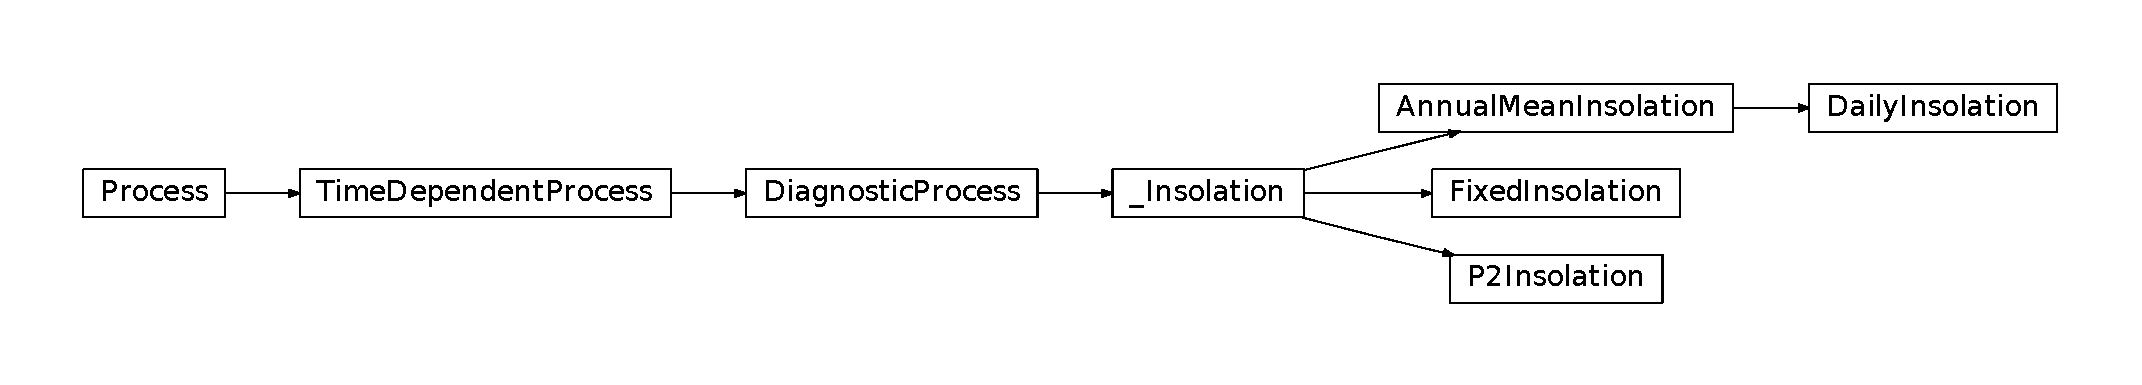
\includegraphics{inheritance-2fabe0d6f5c260b023f1582e871aa6d6b64a2ba8.pdf}
\phantomsection\label{api/climlab.radiation:module-climlab.radiation.insolation}\index{climlab.radiation.insolation (module)}\index{AnnualMeanInsolation (class in climlab.radiation.insolation)}

\begin{fulllineitems}
\phantomsection\label{api/climlab.radiation:climlab.radiation.insolation.AnnualMeanInsolation}\pysiglinewithargsret{\strong{class }\code{climlab.radiation.insolation.}\bfcode{AnnualMeanInsolation}}{\emph{S0=1365.2}, \emph{orb=\{`long\_peri': 281.37}, \emph{`ecc': 0.017236}, \emph{`obliquity': 23.446\}}, \emph{**kwargs}}{}
Bases: {\hyperref[api/climlab.radiation:climlab.radiation.insolation._Insolation]{\emph{\code{climlab.radiation.insolation.\_Insolation}}}} (\autopageref*{api/climlab.radiation:climlab.radiation.insolation._Insolation})

A class for latitudewise solar insolation averaged over a year.

This class computes the solar insolation for each day of the year and 
latitude specified in the domain on the basis of orbital parameters and 
astronomical formulas.

Therefore it uses the method {\hyperref[api/climlab.solar:climlab.solar.insolation.daily_insolation]{\emph{\code{daily\_insolation()}}}} (\autopageref*{api/climlab.solar:climlab.solar.insolation.daily_insolation}).
For details how the solar distribution is dependend on orbital parameters 
see there.

The mean over the year is calculated from data given by
{\hyperref[api/climlab.solar:climlab.solar.insolation.daily_insolation]{\emph{\code{daily\_insolation()}}}} (\autopageref*{api/climlab.solar:climlab.solar.insolation.daily_insolation}) and stored in the 
object's attribute \code{self.insolation}

\textbf{Initialization parameters}
\begin{quote}\begin{description}
\item[{Parameters}] \leavevmode\begin{itemize}
\item {} 
\textbf{\texttt{S0}} (\href{http://docs.python.org/2.7/library/functions.html\#float}{\emph{\texttt{float}}}) -- 
solar constant
\begin{itemize}
\item {} 
unit: \(\frac{\textrm{W}}{\textrm{m}^2}\)

\item {} 
default value: \code{1365.2}

\end{itemize}


\item {} 
\textbf{\texttt{orb}} (\href{http://docs.python.org/2.7/library/stdtypes.html\#dict}{\emph{\texttt{dict}}}) -- 
a dictionary with three orbital parameters (as provided by 
{\hyperref[api/climlab.solar:climlab.solar.orbital.OrbitalTable]{\emph{\code{OrbitalTable}}}} (\autopageref*{api/climlab.solar:climlab.solar.orbital.OrbitalTable})):
\begin{itemize}
\item {} 
\code{'ecc'} - eccentricity
\begin{itemize}
\item {} 
unit: dimensionless

\item {} 
default value: \code{0.017236}

\end{itemize}

\item {} 
\code{'long\_peri'} - longitude of perihelion (precession angle)
\begin{itemize}
\item {} 
unit: degrees

\item {} 
default value: \code{281.37}

\end{itemize}

\item {} 
\code{'obliquity'} - obliquity angle
\begin{itemize}
\item {} 
unit: degrees

\item {} 
default value: \code{23.446}

\end{itemize}

\end{itemize}


\end{itemize}

\end{description}\end{quote}

\textbf{Object attributes}

Additional to the parent class {\hyperref[api/climlab.radiation:climlab.radiation.insolation._Insolation]{\emph{\code{\_Insolation}}}} (\autopageref*{api/climlab.radiation:climlab.radiation.insolation._Insolation})
following object attributes are generated and updated during initialization:
\begin{quote}\begin{description}
\item[{Variables}] \leavevmode\begin{itemize}
\item {} 
{\hyperref[api/climlab.radiation:climlab.radiation.insolation.P2Insolation.insolation]{\emph{\textbf{\texttt{insolation}}}}} (\autopageref*{api/climlab.radiation:climlab.radiation.insolation.P2Insolation.insolation}) ({\hyperref[api/climlab.domain:climlab.domain.field.Field]{\emph{\emph{\texttt{Field}}}}} (\autopageref*{api/climlab.domain:climlab.domain.field.Field})) -- the solar distribution is calculated as a Field on 
the basis of the \code{self.domains{[}'default'{]}} domain
and stored in the attribute \code{self.insolation}.

\item {} 
{\hyperref[api/climlab.radiation:climlab.radiation.insolation.AnnualMeanInsolation.orb]{\emph{\textbf{\texttt{orb}}}}} (\autopageref*{api/climlab.radiation:climlab.radiation.insolation.AnnualMeanInsolation.orb}) (\href{http://docs.python.org/2.7/library/stdtypes.html\#dict}{\emph{\texttt{dict}}}) -- initialized with given argument \code{orb}

\end{itemize}

\item[{Example}] \leavevmode
Create regular EBM and replace standard insolation subprocess by 
\code{AnnualMeanInsolation}:

\begin{Verbatim}[commandchars=\\\{\}]
\PYG{g+gp}{\PYGZgt{}\PYGZgt{}\PYGZgt{} }\PYG{k+kn}{import} \PYG{n+nn}{climlab}
\PYG{g+gp}{\PYGZgt{}\PYGZgt{}\PYGZgt{} }\PYG{k+kn}{from} \PYG{n+nn}{climlab.radiation} \PYG{k+kn}{import} \PYG{n}{AnnualMeanInsolation}

\PYG{g+gp}{\PYGZgt{}\PYGZgt{}\PYGZgt{} }\PYG{c+c1}{\PYGZsh{} model creation}
\PYG{g+gp}{\PYGZgt{}\PYGZgt{}\PYGZgt{} }\PYG{n}{model} \PYG{o}{=} \PYG{n}{climlab}\PYG{o}{.}\PYG{n}{EBM}\PYG{p}{(}\PYG{p}{)}

\PYG{g+gp}{\PYGZgt{}\PYGZgt{}\PYGZgt{} }\PYG{k}{print} \PYG{n}{model}
\end{Verbatim}

\begin{Verbatim}[commandchars=\\\{\}]
climlab Process of type \PYGZlt{}class \PYGZsq{}climlab.model.ebm.EBM\PYGZsq{}\PYGZgt{}. 
State variables and domain shapes: 
  Ts: (90, 1) 
The subprocess tree: 
top: \PYGZlt{}class \PYGZsq{}climlab.model.ebm.EBM\PYGZsq{}\PYGZgt{}
   diffusion: \PYGZlt{}class \PYGZsq{}climlab.dynamics.diffusion.MeridionalDiffusion\PYGZsq{}\PYGZgt{}
   LW: \PYGZlt{}class \PYGZsq{}climlab.radiation.AplusBT.AplusBT\PYGZsq{}\PYGZgt{}
   albedo: \PYGZlt{}class \PYGZsq{}climlab.surface.albedo.StepFunctionAlbedo\PYGZsq{}\PYGZgt{}
      iceline: \PYGZlt{}class \PYGZsq{}climlab.surface.albedo.Iceline\PYGZsq{}\PYGZgt{}
      cold\PYGZus{}albedo: \PYGZlt{}class \PYGZsq{}climlab.surface.albedo.ConstantAlbedo\PYGZsq{}\PYGZgt{}
      warm\PYGZus{}albedo: \PYGZlt{}class \PYGZsq{}climlab.surface.albedo.P2Albedo\PYGZsq{}\PYGZgt{}
   insolation: \PYGZlt{}class \PYGZsq{}climlab.radiation.insolation.P2Insolation\PYGZsq{}\PYGZgt{}
\end{Verbatim}

\begin{Verbatim}[commandchars=\\\{\}]
\PYG{g+gp}{\PYGZgt{}\PYGZgt{}\PYGZgt{} }\PYG{c+c1}{\PYGZsh{} catch model domain for subprocess creation}
\PYG{g+gp}{\PYGZgt{}\PYGZgt{}\PYGZgt{} }\PYG{n}{sfc} \PYG{o}{=} \PYG{n}{model}\PYG{o}{.}\PYG{n}{domains}\PYG{p}{[}\PYG{l+s+s1}{\PYGZsq{}}\PYG{l+s+s1}{Ts}\PYG{l+s+s1}{\PYGZsq{}}\PYG{p}{]}

\PYG{g+gp}{\PYGZgt{}\PYGZgt{}\PYGZgt{} }\PYG{c+c1}{\PYGZsh{} create AnnualMeanInsolation subprocess }
\PYG{g+gp}{\PYGZgt{}\PYGZgt{}\PYGZgt{} }\PYG{n}{new\PYGZus{}insol} \PYG{o}{=} \PYG{n}{AnnualMeanInsolation}\PYG{p}{(}\PYG{n}{domains}\PYG{o}{=}\PYG{n}{sfc}\PYG{p}{,} \PYG{o}{*}\PYG{o}{*}\PYG{n}{model}\PYG{o}{.}\PYG{n}{param}\PYG{p}{)}

\PYG{g+gp}{\PYGZgt{}\PYGZgt{}\PYGZgt{} }\PYG{c+c1}{\PYGZsh{} add it to the model}
\PYG{g+gp}{\PYGZgt{}\PYGZgt{}\PYGZgt{} }\PYG{n}{model}\PYG{o}{.}\PYG{n}{add\PYGZus{}subprocess}\PYG{p}{(}\PYG{l+s+s1}{\PYGZsq{}}\PYG{l+s+s1}{insolation}\PYG{l+s+s1}{\PYGZsq{}}\PYG{p}{,}\PYG{n}{new\PYGZus{}insol}\PYG{p}{)}

\PYG{g+gp}{\PYGZgt{}\PYGZgt{}\PYGZgt{} }\PYG{k}{print} \PYG{n}{model}
\end{Verbatim}

\begin{Verbatim}[commandchars=\\\{\}]
climlab Process of type \PYGZlt{}class \PYGZsq{}climlab.model.ebm.EBM\PYGZsq{}\PYGZgt{}. 
State variables and domain shapes: 
  Ts: (90, 1) 
The subprocess tree: 
top: \PYGZlt{}class \PYGZsq{}climlab.model.ebm.EBM\PYGZsq{}\PYGZgt{}
   diffusion: \PYGZlt{}class \PYGZsq{}climlab.dynamics.diffusion.MeridionalDiffusion\PYGZsq{}\PYGZgt{}
   LW: \PYGZlt{}class \PYGZsq{}climlab.radiation.AplusBT.AplusBT\PYGZsq{}\PYGZgt{}
   albedo: \PYGZlt{}class \PYGZsq{}climlab.surface.albedo.StepFunctionAlbedo\PYGZsq{}\PYGZgt{}
      iceline: \PYGZlt{}class \PYGZsq{}climlab.surface.albedo.Iceline\PYGZsq{}\PYGZgt{}
      cold\PYGZus{}albedo: \PYGZlt{}class \PYGZsq{}climlab.surface.albedo.ConstantAlbedo\PYGZsq{}\PYGZgt{}
      warm\PYGZus{}albedo: \PYGZlt{}class \PYGZsq{}climlab.surface.albedo.P2Albedo\PYGZsq{}\PYGZgt{}
   insolation: \PYGZlt{}class \PYGZsq{}climlab.radiation.insolation.AnnualMeanInsolation\PYGZsq{}\PYGZgt{}
\end{Verbatim}

\end{description}\end{quote}
\index{orb (climlab.radiation.insolation.AnnualMeanInsolation attribute)}

\begin{fulllineitems}
\phantomsection\label{api/climlab.radiation:climlab.radiation.insolation.AnnualMeanInsolation.orb}\pysigline{\bfcode{orb}}
Property of dictionary for orbital parameters.

orb contains: (for more information see {\hyperref[api/climlab.solar:climlab.solar.orbital.OrbitalTable]{\emph{\code{OrbitalTable}}}} (\autopageref*{api/climlab.solar:climlab.solar.orbital.OrbitalTable}))
\begin{itemize}
\item {} 
\code{'ecc'} - eccentricity {[}unit: dimensionless{]}

\item {} 
\code{'long\_peri'} - longitude of perihelion (precession angle) {[}unit: degrees{]}

\item {} 
\code{'obliquity'} - obliquity angle {[}unit: degrees{]}

\end{itemize}
\begin{quote}\begin{description}
\item[{Getter}] \leavevmode
Returns the orbital dictionary which is stored in attribute 
\code{self.\_orb}.

\item[{Setter}] \leavevmode\begin{itemize}
\item {} 
sets orb which is addressed as \code{self.\_orb} to the new value

\item {} 
updates the parameter dictionary \code{self.param{[}'orb'{]}} and

\item {} 
calls method \code{\_compute\_fixed()}

\end{itemize}

\item[{Type}] \leavevmode
dict

\end{description}\end{quote}

\end{fulllineitems}


\end{fulllineitems}

\index{DailyInsolation (class in climlab.radiation.insolation)}

\begin{fulllineitems}
\phantomsection\label{api/climlab.radiation:climlab.radiation.insolation.DailyInsolation}\pysiglinewithargsret{\strong{class }\code{climlab.radiation.insolation.}\bfcode{DailyInsolation}}{\emph{S0=1365.2}, \emph{orb=\{`long\_peri': 281.37}, \emph{`ecc': 0.017236}, \emph{`obliquity': 23.446\}}, \emph{**kwargs}}{}
Bases: {\hyperref[api/climlab.radiation:climlab.radiation.insolation.AnnualMeanInsolation]{\emph{\code{climlab.radiation.insolation.AnnualMeanInsolation}}}} (\autopageref*{api/climlab.radiation:climlab.radiation.insolation.AnnualMeanInsolation})

A class to compute latitudewise daily solar insolation for specific 
days of the year.

This class computes the solar insolation on basis of orbital parameters and 
astronomical formulas.

Therefore it uses the method {\hyperref[api/climlab.solar:climlab.solar.insolation.daily_insolation]{\emph{\code{daily\_insolation()}}}} (\autopageref*{api/climlab.solar:climlab.solar.insolation.daily_insolation}).
For details how the solar distribution is dependend on orbital parameters 
see there.

\textbf{Initialization parameters}
\begin{quote}\begin{description}
\item[{Parameters}] \leavevmode\begin{itemize}
\item {} 
\textbf{\texttt{S0}} (\href{http://docs.python.org/2.7/library/functions.html\#float}{\emph{\texttt{float}}}) -- 
solar constant
\begin{itemize}
\item {} 
unit: \(\frac{\textrm{W}}{\textrm{m}^2}\)

\item {} 
default value: \code{1365.2}

\end{itemize}


\item {} 
\textbf{\texttt{orb}} (\href{http://docs.python.org/2.7/library/stdtypes.html\#dict}{\emph{\texttt{dict}}}) -- 
a dictionary with orbital parameters:
\begin{itemize}
\item {} 
\code{'ecc'} - eccentricity
\begin{itemize}
\item {} 
unit: dimensionless

\item {} 
default value: \code{0.017236}

\end{itemize}

\item {} 
\code{'long\_peri'} - longitude of perihelion (precession angle)
\begin{itemize}
\item {} 
unit: degrees

\item {} 
default value: \code{281.37}

\end{itemize}

\item {} 
\code{'obliquity'} - obliquity angle
\begin{itemize}
\item {} 
unit: degrees

\item {} 
default value: \code{23.446}

\end{itemize}

\end{itemize}


\end{itemize}

\end{description}\end{quote}

\textbf{Object attributes}

Additional to the parent class {\hyperref[api/climlab.radiation:climlab.radiation.insolation._Insolation]{\emph{\code{\_Insolation}}}} (\autopageref*{api/climlab.radiation:climlab.radiation.insolation._Insolation})
following object attributes are generated and updated during initialization:
\begin{quote}\begin{description}
\item[{Variables}] \leavevmode\begin{itemize}
\item {} 
{\hyperref[api/climlab.radiation:climlab.radiation.insolation.P2Insolation.insolation]{\emph{\textbf{\texttt{insolation}}}}} (\autopageref*{api/climlab.radiation:climlab.radiation.insolation.P2Insolation.insolation}) ({\hyperref[api/climlab.domain:climlab.domain.field.Field]{\emph{\emph{\texttt{Field}}}}} (\autopageref*{api/climlab.domain:climlab.domain.field.Field})) -- the solar distribution is calculated as a Field on 
the basis of the \code{self.domains{[}'default'{]}} domain
and stored in the attribute \code{self.insolation}.

\item {} 
{\hyperref[api/climlab.radiation:climlab.radiation.insolation.AnnualMeanInsolation.orb]{\emph{\textbf{\texttt{orb}}}}} (\autopageref*{api/climlab.radiation:climlab.radiation.insolation.AnnualMeanInsolation.orb}) (\href{http://docs.python.org/2.7/library/stdtypes.html\#dict}{\emph{\texttt{dict}}}) -- initialized with given argument \code{orb}

\end{itemize}

\item[{Example}] \leavevmode
Create regular EBM and replace standard insolation subprocess by 
\code{DailyInsolation}:

\begin{Verbatim}[commandchars=\\\{\}]
\PYG{g+gp}{\PYGZgt{}\PYGZgt{}\PYGZgt{} }\PYG{k+kn}{import} \PYG{n+nn}{climlab}
\PYG{g+gp}{\PYGZgt{}\PYGZgt{}\PYGZgt{} }\PYG{k+kn}{from} \PYG{n+nn}{climlab.radiation} \PYG{k+kn}{import} \PYG{n}{DailyInsolation}

\PYG{g+gp}{\PYGZgt{}\PYGZgt{}\PYGZgt{} }\PYG{c+c1}{\PYGZsh{} model creation}
\PYG{g+gp}{\PYGZgt{}\PYGZgt{}\PYGZgt{} }\PYG{n}{model} \PYG{o}{=} \PYG{n}{climlab}\PYG{o}{.}\PYG{n}{EBM}\PYG{p}{(}\PYG{p}{)}

\PYG{g+gp}{\PYGZgt{}\PYGZgt{}\PYGZgt{} }\PYG{k}{print} \PYG{n}{model}
\end{Verbatim}

\begin{Verbatim}[commandchars=\\\{\}]
climlab Process of type \PYGZlt{}class \PYGZsq{}climlab.model.ebm.EBM\PYGZsq{}\PYGZgt{}. 
State variables and domain shapes: 
  Ts: (90, 1) 
The subprocess tree: 
top: \PYGZlt{}class \PYGZsq{}climlab.model.ebm.EBM\PYGZsq{}\PYGZgt{}
   diffusion: \PYGZlt{}class \PYGZsq{}climlab.dynamics.diffusion.MeridionalDiffusion\PYGZsq{}\PYGZgt{}
   LW: \PYGZlt{}class \PYGZsq{}climlab.radiation.AplusBT.AplusBT\PYGZsq{}\PYGZgt{}
   albedo: \PYGZlt{}class \PYGZsq{}climlab.surface.albedo.StepFunctionAlbedo\PYGZsq{}\PYGZgt{}
      iceline: \PYGZlt{}class \PYGZsq{}climlab.surface.albedo.Iceline\PYGZsq{}\PYGZgt{}
      cold\PYGZus{}albedo: \PYGZlt{}class \PYGZsq{}climlab.surface.albedo.ConstantAlbedo\PYGZsq{}\PYGZgt{}
      warm\PYGZus{}albedo: \PYGZlt{}class \PYGZsq{}climlab.surface.albedo.P2Albedo\PYGZsq{}\PYGZgt{}
   insolation: \PYGZlt{}class \PYGZsq{}climlab.radiation.insolation.P2Insolation\PYGZsq{}\PYGZgt{}
\end{Verbatim}

\begin{Verbatim}[commandchars=\\\{\}]
\PYG{g+gp}{\PYGZgt{}\PYGZgt{}\PYGZgt{} }\PYG{c+c1}{\PYGZsh{} catch model domain for subprocess creation}
\PYG{g+gp}{\PYGZgt{}\PYGZgt{}\PYGZgt{} }\PYG{n}{sfc} \PYG{o}{=} \PYG{n}{model}\PYG{o}{.}\PYG{n}{domains}\PYG{p}{[}\PYG{l+s+s1}{\PYGZsq{}}\PYG{l+s+s1}{Ts}\PYG{l+s+s1}{\PYGZsq{}}\PYG{p}{]}

\PYG{g+gp}{\PYGZgt{}\PYGZgt{}\PYGZgt{} }\PYG{c+c1}{\PYGZsh{} create DailyInsolation subprocess and add it to the model}
\PYG{g+gp}{\PYGZgt{}\PYGZgt{}\PYGZgt{} }\PYG{n}{model}\PYG{o}{.}\PYG{n}{add\PYGZus{}subprocess}\PYG{p}{(}\PYG{l+s+s1}{\PYGZsq{}}\PYG{l+s+s1}{insolation}\PYG{l+s+s1}{\PYGZsq{}}\PYG{p}{,}\PYG{n}{DailyInsolation}\PYG{p}{(}\PYG{n}{domains}\PYG{o}{=}\PYG{n}{sfc}\PYG{p}{,} \PYG{o}{*}\PYG{o}{*}\PYG{n}{model}\PYG{o}{.}\PYG{n}{param}\PYG{p}{)}\PYG{p}{)}

\PYG{g+gp}{\PYGZgt{}\PYGZgt{}\PYGZgt{} }\PYG{k}{print} \PYG{n}{model}
\end{Verbatim}

\begin{Verbatim}[commandchars=\\\{\}]
climlab Process of type \PYGZlt{}class \PYGZsq{}climlab.model.ebm.EBM\PYGZsq{}\PYGZgt{}. 
State variables and domain shapes: 
  Ts: (90, 1) 
The subprocess tree: 
top: \PYGZlt{}class \PYGZsq{}climlab.model.ebm.EBM\PYGZsq{}\PYGZgt{}
   diffusion: \PYGZlt{}class \PYGZsq{}climlab.dynamics.diffusion.MeridionalDiffusion\PYGZsq{}\PYGZgt{}
   LW: \PYGZlt{}class \PYGZsq{}climlab.radiation.AplusBT.AplusBT\PYGZsq{}\PYGZgt{}
   albedo: \PYGZlt{}class \PYGZsq{}climlab.surface.albedo.StepFunctionAlbedo\PYGZsq{}\PYGZgt{}
      iceline: \PYGZlt{}class \PYGZsq{}climlab.surface.albedo.Iceline\PYGZsq{}\PYGZgt{}
      cold\PYGZus{}albedo: \PYGZlt{}class \PYGZsq{}climlab.surface.albedo.ConstantAlbedo\PYGZsq{}\PYGZgt{}
      warm\PYGZus{}albedo: \PYGZlt{}class \PYGZsq{}climlab.surface.albedo.P2Albedo\PYGZsq{}\PYGZgt{}
   insolation: \PYGZlt{}class \PYGZsq{}climlab.radiation.insolation.DailyInsolation\PYGZsq{}\PYGZgt{}
\end{Verbatim}

\end{description}\end{quote}
\index{insolation (climlab.radiation.insolation.DailyInsolation attribute)}

\begin{fulllineitems}
\phantomsection\label{api/climlab.radiation:climlab.radiation.insolation.DailyInsolation.insolation}\pysigline{\bfcode{insolation}}
\end{fulllineitems}


\end{fulllineitems}

\index{FixedInsolation (class in climlab.radiation.insolation)}

\begin{fulllineitems}
\phantomsection\label{api/climlab.radiation:climlab.radiation.insolation.FixedInsolation}\pysiglinewithargsret{\strong{class }\code{climlab.radiation.insolation.}\bfcode{FixedInsolation}}{\emph{S0=341.3}, \emph{**kwargs}}{}
Bases: {\hyperref[api/climlab.radiation:climlab.radiation.insolation._Insolation]{\emph{\code{climlab.radiation.insolation.\_Insolation}}}} (\autopageref*{api/climlab.radiation:climlab.radiation.insolation._Insolation})

A class for fixed insolation at each point of latitude off the domain.

The solar distribution for the whole domain is constant and specified by
a parameter.

\textbf{Initialization parameters}
\begin{quote}\begin{description}
\item[{Parameters}] \leavevmode
\textbf{\texttt{S0}} (\href{http://docs.python.org/2.7/library/functions.html\#float}{\emph{\texttt{float}}}) -- 
solar constant
\begin{itemize}
\item {} 
unit: \(\frac{\textrm{W}}{\textrm{m}^2}\)

\item {} 
default value: \code{const.S0/4 = 341.2}

\end{itemize}


\item[{Example}] \leavevmode
\begin{Verbatim}[commandchars=\\\{\}]
\PYG{g+gp}{\PYGZgt{}\PYGZgt{}\PYGZgt{} }\PYG{k+kn}{import} \PYG{n+nn}{climlab}
\PYG{g+gp}{\PYGZgt{}\PYGZgt{}\PYGZgt{} }\PYG{k+kn}{from} \PYG{n+nn}{climlab.radiation.insolation} \PYG{k+kn}{import} \PYG{n}{FixedInsolation}

\PYG{g+gp}{\PYGZgt{}\PYGZgt{}\PYGZgt{} }\PYG{n}{model} \PYG{o}{=} \PYG{n}{climlab}\PYG{o}{.}\PYG{n}{EBM}\PYG{p}{(}\PYG{p}{)}
\PYG{g+gp}{\PYGZgt{}\PYGZgt{}\PYGZgt{} }\PYG{n}{sfc} \PYG{o}{=} \PYG{n}{model}\PYG{o}{.}\PYG{n}{Ts}\PYG{o}{.}\PYG{n}{domain}

\PYG{g+gp}{\PYGZgt{}\PYGZgt{}\PYGZgt{} }\PYG{n}{fixed\PYGZus{}ins} \PYG{o}{=} \PYG{n}{FixedInsolation}\PYG{p}{(}\PYG{n}{S0}\PYG{o}{=}\PYG{l+m+mf}{340.0}\PYG{p}{,} \PYG{n}{domains}\PYG{o}{=}\PYG{n}{sfc}\PYG{p}{)}

\PYG{g+gp}{\PYGZgt{}\PYGZgt{}\PYGZgt{} }\PYG{k}{print} \PYG{n}{fixed\PYGZus{}ins}
\PYG{g+go}{climlab Process of type \PYGZlt{}class \PYGZsq{}climlab.radiation.insolation.FixedInsolation\PYGZsq{}\PYGZgt{}. }
\PYG{g+go}{State variables and domain shapes: }
\PYG{g+go}{The subprocess tree: }
\PYG{g+go}{top: \PYGZlt{}class \PYGZsq{}climlab.radiation.insolation.FixedInsolation\PYGZsq{}\PYGZgt{}}
\end{Verbatim}

\end{description}\end{quote}
\index{insolation (climlab.radiation.insolation.FixedInsolation attribute)}

\begin{fulllineitems}
\phantomsection\label{api/climlab.radiation:climlab.radiation.insolation.FixedInsolation.insolation}\pysigline{\bfcode{insolation}}
\end{fulllineitems}


\end{fulllineitems}

\index{P2Insolation (class in climlab.radiation.insolation)}

\begin{fulllineitems}
\phantomsection\label{api/climlab.radiation:climlab.radiation.insolation.P2Insolation}\pysiglinewithargsret{\strong{class }\code{climlab.radiation.insolation.}\bfcode{P2Insolation}}{\emph{S0=1365.2}, \emph{s2=-0.48}, \emph{**kwargs}}{}
Bases: {\hyperref[api/climlab.radiation:climlab.radiation.insolation._Insolation]{\emph{\code{climlab.radiation.insolation.\_Insolation}}}} (\autopageref*{api/climlab.radiation:climlab.radiation.insolation._Insolation})

A class for parabolic solar distribution over the domain's latitude 
on the basis of the second order Legendre Polynomial.

Calculates the latitude dependent solar distribution as
\begin{gather}
\begin{split}S(\varphi) = \frac{S_0}{4} \left( 1 + s_2 P_2(x) \right)\end{split}\notag
\end{gather}
where \(P_2(x) = \frac{1}{2} (3x^2 - 1)\) is the second order Legendre Polynomial
and \(x=sin(\varphi)\).

\textbf{Initialization parameters}
\begin{quote}\begin{description}
\item[{Parameters}] \leavevmode\begin{itemize}
\item {} 
\textbf{\texttt{S0}} (\href{http://docs.python.org/2.7/library/functions.html\#float}{\emph{\texttt{float}}}) -- 
solar constant
\begin{itemize}
\item {} 
unit: \(\frac{\textrm{W}}{\textrm{m}^2}\)

\item {} 
default value: \code{1365.2}

\end{itemize}


\item {} 
\textbf{\texttt{s2}} (\emph{\texttt{floar}}) -- 
factor for second legendre polynominal term
\begin{itemize}
\item {} 
default value: \code{-0.48}

\end{itemize}


\end{itemize}

\item[{Example}] \leavevmode
\begin{Verbatim}[commandchars=\\\{\}]
\PYG{g+gp}{\PYGZgt{}\PYGZgt{}\PYGZgt{} }\PYG{k+kn}{import} \PYG{n+nn}{climlab}
\PYG{g+gp}{\PYGZgt{}\PYGZgt{}\PYGZgt{} }\PYG{k+kn}{from} \PYG{n+nn}{climlab.radiation.insolation} \PYG{k+kn}{import} \PYG{n}{P2Insolation}

\PYG{g+gp}{\PYGZgt{}\PYGZgt{}\PYGZgt{} }\PYG{n}{model} \PYG{o}{=} \PYG{n}{climlab}\PYG{o}{.}\PYG{n}{EBM}\PYG{p}{(}\PYG{p}{)}
\PYG{g+gp}{\PYGZgt{}\PYGZgt{}\PYGZgt{} }\PYG{n}{sfc} \PYG{o}{=} \PYG{n}{model}\PYG{o}{.}\PYG{n}{Ts}\PYG{o}{.}\PYG{n}{domain}

\PYG{g+gp}{\PYGZgt{}\PYGZgt{}\PYGZgt{} }\PYG{n}{p2\PYGZus{}ins} \PYG{o}{=} \PYG{n}{P2Insolation}\PYG{p}{(}\PYG{n}{S0}\PYG{o}{=}\PYG{l+m+mf}{340.0}\PYG{p}{,} \PYG{n}{s2}\PYG{o}{=}\PYG{o}{\PYGZhy{}}\PYG{l+m+mf}{0.5}\PYG{p}{,} \PYG{n}{domains}\PYG{o}{=}\PYG{n}{sfc}\PYG{p}{)}

\PYG{g+gp}{\PYGZgt{}\PYGZgt{}\PYGZgt{} }\PYG{k}{print} \PYG{n}{p2\PYGZus{}ins}
\PYG{g+go}{climlab Process of type \PYGZlt{}class \PYGZsq{}climlab.radiation.insolation.P2Insolation\PYGZsq{}\PYGZgt{}. }
\PYG{g+go}{State variables and domain shapes: }
\PYG{g+go}{The subprocess tree: }
\PYG{g+go}{top: \PYGZlt{}class \PYGZsq{}climlab.radiation.insolation.P2Insolation\PYGZsq{}\PYGZgt{}    }
\end{Verbatim}

\end{description}\end{quote}
\index{insolation (climlab.radiation.insolation.P2Insolation attribute)}

\begin{fulllineitems}
\phantomsection\label{api/climlab.radiation:climlab.radiation.insolation.P2Insolation.insolation}\pysigline{\bfcode{insolation}}
\end{fulllineitems}

\index{s2 (climlab.radiation.insolation.P2Insolation attribute)}

\begin{fulllineitems}
\phantomsection\label{api/climlab.radiation:climlab.radiation.insolation.P2Insolation.s2}\pysigline{\bfcode{s2}}
Property of second legendre polynomial factor s2.

s2 in following equation:
\begin{gather}
\begin{split}S(\varphi) = \frac{S_0}{4} \left( 1 + s_2 P_2(x) \right)\end{split}\notag
\end{gather}\begin{quote}\begin{description}
\item[{Getter}] \leavevmode
Returns the s2 parameter which is stored in attribute \code{self.\_s2}.

\item[{Setter}] \leavevmode\begin{itemize}
\item {} 
sets s2 which is addressed as \code{self.\_S0} to the new value

\item {} 
updates the parameter dictionary \code{self.param{[}'s2'{]}} and

\item {} 
calls method \code{\_compute\_fixed()}

\end{itemize}

\item[{Type}] \leavevmode
float

\end{description}\end{quote}

\end{fulllineitems}


\end{fulllineitems}

\index{\_Insolation (class in climlab.radiation.insolation)}

\begin{fulllineitems}
\phantomsection\label{api/climlab.radiation:climlab.radiation.insolation._Insolation}\pysiglinewithargsret{\strong{class }\code{climlab.radiation.insolation.}\bfcode{\_Insolation}}{\emph{S0=1365.2}, \emph{**kwargs}}{}
Bases: {\hyperref[api/climlab.process:climlab.process.diagnostic.DiagnosticProcess]{\emph{\code{climlab.process.diagnostic.DiagnosticProcess}}}} (\autopageref*{api/climlab.process:climlab.process.diagnostic.DiagnosticProcess})

A private parent class for insolation processes.

Calling compute() will update self.insolation with current values.

\textbf{Initialization parameters}

An instance of \code{\_Insolation} is initialized with the following 
arguments \emph{(for detailed information see Object attributes below)}:
\begin{quote}\begin{description}
\item[{Parameters}] \leavevmode
\textbf{\texttt{S0}} (\href{http://docs.python.org/2.7/library/functions.html\#float}{\emph{\texttt{float}}}) -- 
solar constant
\begin{itemize}
\item {} 
unit: \(\frac{\textrm{W}}{\textrm{m}^2}\)

\item {} 
default value: \code{1365.2}

\end{itemize}


\end{description}\end{quote}

\textbf{Object attributes}

Additional to the parent class {\hyperref[api/climlab.process:climlab.process.diagnostic.DiagnosticProcess]{\emph{\code{DiagnosticProcess}}}} (\autopageref*{api/climlab.process:climlab.process.diagnostic.DiagnosticProcess})
following object attributes are generated and updated during initialization:
\begin{quote}\begin{description}
\item[{Variables}] \leavevmode\begin{itemize}
\item {} 
{\hyperref[api/climlab.radiation:climlab.radiation.insolation.P2Insolation.insolation]{\emph{\textbf{\texttt{insolation}}}}} (\autopageref*{api/climlab.radiation:climlab.radiation.insolation.P2Insolation.insolation}) ({\hyperref[api/climlab.domain:climlab.domain.field.Field]{\emph{\emph{\texttt{Field}}}}} (\autopageref*{api/climlab.domain:climlab.domain.field.Field})) -- the array is initialized with zeros of the size of
\code{self.domains{[}'sfc'{]}} or \code{self.domains{[}'default'{]}}.

\item {} 
{\hyperref[api/climlab.radiation:climlab.radiation.insolation._Insolation.S0]{\emph{\textbf{\texttt{S0}}}}} (\autopageref*{api/climlab.radiation:climlab.radiation.insolation._Insolation.S0}) (\href{http://docs.python.org/2.7/library/functions.html\#float}{\emph{\texttt{float}}}) -- initialized with given argument \code{S0}

\item {} 
\textbf{\texttt{diagnostics}} (\href{http://docs.python.org/2.7/library/stdtypes.html\#dict}{\emph{\texttt{dict}}}) -- key \code{'insolation'} initialized with value:
{\hyperref[api/climlab.domain:climlab.domain.field.Field]{\emph{\code{Field}}}} (\autopageref*{api/climlab.domain:climlab.domain.field.Field}) of zeros
in size of \code{self.domains{[}'sfc'{]}} or
\code{self.domains{[}'default'{]}}

\item {} 
{\hyperref[api/climlab.radiation:climlab.radiation.insolation.P2Insolation.insolation]{\emph{\textbf{\texttt{insolation}}}}} (\autopageref*{api/climlab.radiation:climlab.radiation.insolation.P2Insolation.insolation}) -- the subprocess attribute \code{self.insolation} is
created with correct dimensions

\end{itemize}

\end{description}\end{quote}

\begin{notice}{note}{Note:}
\code{self.insolation} should always be modified with 
\code{self.insolation{[}:{]} = ...} so that links to the insolation in other
processes will work.
\end{notice}
\index{S0 (climlab.radiation.insolation.\_Insolation attribute)}

\begin{fulllineitems}
\phantomsection\label{api/climlab.radiation:climlab.radiation.insolation._Insolation.S0}\pysigline{\bfcode{S0}}
Property of solar constant S0.

The parameter S0 is stored using a python property and can be changed through 
\code{self.S0 = newvalue} which will also update the parameter dictionary.

\begin{notice}{warning}{Warning:}
changing \code{self.param{[}'S0'{]}} will not work!
\end{notice}
\begin{quote}\begin{description}
\item[{Getter}] \leavevmode
Returns the S0 parameter which is stored in attribute \code{self.\_S0}.

\item[{Setter}] \leavevmode\begin{itemize}
\item {} 
sets S0 which is addressed as \code{self.\_S0} to the new value

\item {} 
updates the parameter dictionary \code{self.param{[}'S0'{]}} and

\item {} 
calls method \code{\_compute\_fixed()}

\end{itemize}

\item[{Type}] \leavevmode
float

\end{description}\end{quote}

\end{fulllineitems}


\end{fulllineitems}



\subsection{climlab.solar package}
\label{api/climlab.solar::doc}\label{api/climlab.solar:climlab-solar-package}

\subsubsection{climlab.solar.insolation module}
\label{api/climlab.solar:module-climlab.solar.insolation}\label{api/climlab.solar:climlab-solar-insolation-module}\index{climlab.solar.insolation (module)}
This module contains general-purpose routines for computing incoming
solar radiation at the top of the atmosphere.

Currently, only daily average insolation is computed.

\begin{notice}{note}{Note:}
Ported and modified from MATLAB code daily\_insolation.m

\emph{Original authors:}
\begin{quote}

Ian Eisenman and Peter Huybers, Harvard University, August 2006
\end{quote}

Available online at \href{http://eisenman.ucsd.edu/code/daily\_insolation.m}{http://eisenman.ucsd.edu/code/daily\_insolation.m}
\end{notice}

If using calendar days, solar longitude is found using an
approximate solution to the differential equation representing conservation
of angular momentum (Kepler's Second Law).  Given the orbital parameters
and solar longitude, daily average insolation is calculated exactly
following {[}Berger\_1978{]}. Further references: {[}Berger\_1991{]}.
\index{daily\_insolation() (in module climlab.solar.insolation)}

\begin{fulllineitems}
\phantomsection\label{api/climlab.solar:climlab.solar.insolation.daily_insolation}\pysiglinewithargsret{\code{climlab.solar.insolation.}\bfcode{daily\_insolation}}{\emph{lat}, \emph{day}, \emph{orb=\{`long\_peri': 281.37}, \emph{`ecc': 0.017236}, \emph{`obliquity': 23.446\}}, \emph{S0=None}, \emph{day\_type=1}}{}
Compute daily average insolation given latitude, time of year and orbital parameters.

Orbital parameters can be computed for any time in the last 5 Myears with
{\hyperref[api/climlab.solar:climlab.solar.orbital.OrbitalTable.lookup_parameters]{\emph{\code{lookup\_parameters()}}}} (\autopageref*{api/climlab.solar:climlab.solar.orbital.OrbitalTable.lookup_parameters}) (see example below).

\textbf{Function-call argument}
\begin{quote}\begin{description}
\item[{Parameters}] \leavevmode\begin{itemize}
\item {} 
\textbf{\texttt{lat}} (\href{http://docs.python.org/2.7/library/array.html\#module-array}{\emph{\texttt{array}}}) -- Latitude in degrees (-90 to 90).

\item {} 
\textbf{\texttt{day}} (\href{http://docs.python.org/2.7/library/array.html\#module-array}{\emph{\texttt{array}}}) -- Indicator of time of year. See argument \code{day\_type}
for details about format.

\item {} 
\textbf{\texttt{orb}} (\href{http://docs.python.org/2.7/library/stdtypes.html\#dict}{\emph{\texttt{dict}}}) -- 
a dictionary with three members (as provided by 
{\hyperref[api/climlab.solar:climlab.solar.orbital.OrbitalTable]{\emph{\code{OrbitalTable}}}} (\autopageref*{api/climlab.solar:climlab.solar.orbital.OrbitalTable}))
\begin{itemize}
\item {} 
\code{'ecc'} - eccentricity
\begin{itemize}
\item {} 
unit: dimensionless

\item {} 
default value: \code{0.017236}

\end{itemize}

\item {} 
\code{'long\_peri'} - longitude of perihelion (precession angle)
\begin{itemize}
\item {} 
unit: degrees

\item {} 
default value: \code{281.37}

\end{itemize}

\item {} 
\code{'obliquity'} - obliquity angle
\begin{itemize}
\item {} 
unit: degrees

\item {} 
default value: \code{23.446}

\end{itemize}

\end{itemize}


\item {} 
\textbf{\texttt{S0}} (\href{http://docs.python.org/2.7/library/functions.html\#float}{\emph{\texttt{float}}}) -- 
solar constant
\begin{itemize}
\item {} 
unit: \(\textrm{W}/\textrm{m}^2\)

\item {} 
default value: \code{1365.2}

\end{itemize}


\item {} 
\textbf{\texttt{day\_type}} (\href{http://docs.python.org/2.7/library/functions.html\#int}{\emph{\texttt{int}}}) -- 
Convention for specifying time of year (+/- 1,2) {[}optional{]}.
\begin{description}
\item[{\emph{day\_type=1} (default):}] \leavevmode
day input is calendar day (1-365.24), where day 1
is January first. The calendar is referenced to the 
vernal equinox which always occurs at day 80.

\item[{\emph{day\_type=2:} }] \leavevmode
day input is solar longitude (0-360 degrees). Solar
longitude is the angle of the Earth's orbit measured from spring
equinox (21 March). Note that calendar days and solar longitude are
not linearly related because, by Kepler's Second Law, Earth's
angular velocity varies according to its distance from the sun.

\end{description}


\end{itemize}

\item[{Raises}] \leavevmode
\code{ValueError}
if day\_type is neither 1 nor 2

\item[{Returns}] \leavevmode

Daily average solar radiation in unit 
\(\textrm{W}/\textrm{m}^2\).

Dimensions of output are \code{(lat.size, day.size, ecc.size)}


\item[{Return type}] \leavevmode
\href{http://docs.python.org/2.7/library/array.html\#module-array}{array}

\end{description}\end{quote}

Code is fully vectorized to handle array input for all arguments.

Orbital arguments should all have the same sizes.
This is automatic if computed from 
{\hyperref[api/climlab.solar:climlab.solar.orbital.OrbitalTable.lookup_parameters]{\emph{\code{lookup\_parameters()}}}} (\autopageref*{api/climlab.solar:climlab.solar.orbital.OrbitalTable.lookup_parameters})
\begin{quote}\begin{description}
\item[{Example}] \leavevmode
to compute the timeseries of insolation at 65N at summer
solstice over the past 5 Myears:

\begin{Verbatim}[commandchars=\\\{\}]
\PYG{k+kn}{from} \PYG{n+nn}{climlab.solar.orbital} \PYG{k+kn}{import} \PYG{n}{OrbitalTable}
\PYG{k+kn}{from} \PYG{n+nn}{climlab.solar.insolation} \PYG{k+kn}{import} \PYG{n}{daily\PYGZus{}insolation}

\PYG{c+c1}{\PYGZsh{} import orbital table}
\PYG{n}{table} \PYG{o}{=} \PYG{n}{OrbitalTable}\PYG{p}{(}\PYG{p}{)}

\PYG{c+c1}{\PYGZsh{} array with specified kyears }
\PYG{n}{years} \PYG{o}{=} \PYG{n}{np}\PYG{o}{.}\PYG{n}{linspace}\PYG{p}{(}\PYG{o}{\PYGZhy{}}\PYG{l+m+mi}{5000}\PYG{p}{,} \PYG{l+m+mi}{0}\PYG{p}{,} \PYG{l+m+mi}{5001}\PYG{p}{)}

\PYG{c+c1}{\PYGZsh{} orbital parameters for specified time}
\PYG{n}{orb} \PYG{o}{=} \PYG{n}{table}\PYG{o}{.}\PYG{n}{lookup\PYGZus{}parameters}\PYG{p}{(} \PYG{n}{years} \PYG{p}{)}

\PYG{c+c1}{\PYGZsh{} insolation values for past 5 Myears at 65N at summer solstice}
\PYG{n}{S65} \PYG{o}{=} \PYG{n}{daily\PYGZus{}insolation}\PYG{p}{(} \PYG{l+m+mi}{65}\PYG{p}{,} \PYG{l+m+mi}{172}\PYG{p}{,} \PYG{n}{orb} \PYG{p}{)}
\end{Verbatim}

For more information about computation of solar insolation see the
{\hyperref[tutorial:tutorial]{\emph{Tutorials}}} (\autopageref*{tutorial:tutorial}) chapter.

\end{description}\end{quote}

\end{fulllineitems}

\index{solar\_longitude() (in module climlab.solar.insolation)}

\begin{fulllineitems}
\phantomsection\label{api/climlab.solar:climlab.solar.insolation.solar_longitude}\pysiglinewithargsret{\code{climlab.solar.insolation.}\bfcode{solar\_longitude}}{\emph{day}, \emph{orb=\{`long\_peri': 281.37}, \emph{`ecc': 0.017236}, \emph{`obliquity': 23.446\}}, \emph{days\_per\_year=None}}{}
Estimates solar longitude from calendar day.

Method is using an approximation from {[}Berger\_1978{]} section 3
(lambda = 0 at spring equinox).

\textbf{Function-call arguments}
\begin{quote}\begin{description}
\item[{Parameters}] \leavevmode\begin{itemize}
\item {} 
\textbf{\texttt{day}} (\href{http://docs.python.org/2.7/library/array.html\#module-array}{\emph{\texttt{array}}}) -- Indicator of time of year.

\item {} 
\textbf{\texttt{orb}} (\href{http://docs.python.org/2.7/library/stdtypes.html\#dict}{\emph{\texttt{dict}}}) -- 
a dictionary with three members (as provided by 
{\hyperref[api/climlab.solar:climlab.solar.orbital.OrbitalTable]{\emph{\code{OrbitalTable}}}} (\autopageref*{api/climlab.solar:climlab.solar.orbital.OrbitalTable}))
\begin{itemize}
\item {} 
\code{'ecc'} - eccentricity
\begin{itemize}
\item {} 
unit: dimensionless

\item {} 
default value: \code{0.017236}

\end{itemize}

\item {} 
\code{'long\_peri'} - longitude of perihelion 
(precession angle)
\begin{itemize}
\item {} 
unit: degrees

\item {} 
default value: \code{281.37}

\end{itemize}

\item {} 
\code{'obliquity'} - obliquity angle
\begin{itemize}
\item {} 
unit: degrees

\item {} 
default value: \code{23.446}

\end{itemize}

\end{itemize}


\item {} 
\textbf{\texttt{days\_per\_year}} (\href{http://docs.python.org/2.7/library/functions.html\#float}{\emph{\texttt{float}}}) -- number of days in a year (optional) 
(default: 365.2422)
Reads the length of the year from 
{\hyperref[api/climlab.utils:module\string-climlab.utils.constants]{\emph{\code{constants}}}} (\autopageref*{api/climlab.utils:module-climlab.utils.constants}) if available.

\end{itemize}

\item[{Returns}] \leavevmode
solar longitude \code{lambda\_long}
in dimension{}`{}`( day.size, ecc.size ){}`{}`

\item[{Return type}] \leavevmode
\href{http://docs.python.org/2.7/library/array.html\#module-array}{array}

\end{description}\end{quote}

Works for both scalar and vector orbital parameters.

\end{fulllineitems}



\subsubsection{climlab.solar.orbital module}
\label{api/climlab.solar:climlab-solar-orbital-module}
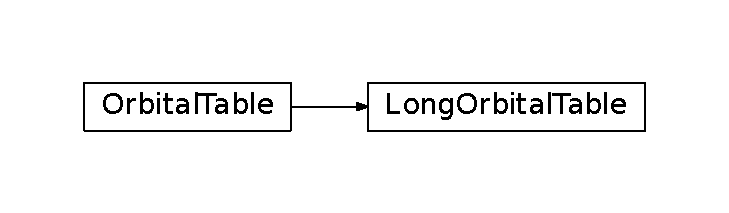
\includegraphics{inheritance-a4659f72efbfa1da05c43c93e29674e4f4358872.pdf}
\phantomsection\label{api/climlab.solar:module-climlab.solar.orbital}\index{climlab.solar.orbital (module)}
This module defines the class {\hyperref[api/climlab.solar:climlab.solar.orbital.OrbitalTable]{\emph{\code{OrbitalTable}}}} (\autopageref*{api/climlab.solar:climlab.solar.orbital.OrbitalTable}) which holds orbital data,
and includes a method {\hyperref[api/climlab.solar:climlab.solar.orbital.OrbitalTable.lookup_parameters]{\emph{\code{lookup\_parameters()}}}} (\autopageref*{api/climlab.solar:climlab.solar.orbital.OrbitalTable.lookup_parameters}) 
which interpolates the orbital data for a specific year 
(- works equally well for arrays of years).

The base class {\hyperref[api/climlab.solar:climlab.solar.orbital.OrbitalTable]{\emph{\code{OrbitalTable()}}}} (\autopageref*{api/climlab.solar:climlab.solar.orbital.OrbitalTable}) is designed to work with 5 Myears of orbital data
(\textbf{eccentricity, obliquity, and longitude of perihelion}) from {[}Berger\_1991{]}.

Data will be read from the file orbit91, which was originally obtained from
\href{ftp://ftp.ncdc.noaa.gov/pub/data/paleo/insolation/}{ftp://ftp.ncdc.noaa.gov/pub/data/paleo/insolation/}
If the file isn't found locally, the module will attempt to read it remotely
from the above URL.

A subclass {\hyperref[api/climlab.solar:climlab.solar.orbital.LongOrbitalTable]{\emph{\code{LongOrbitalTable()}}}} (\autopageref*{api/climlab.solar:climlab.solar.orbital.LongOrbitalTable}) works with La2004 orbital data for 
-51 to +21 Myears as calculated by {[}Laskar\_2004{]}.
See \href{http://vo.imcce.fr/insola/earth/online/earth/La2004/README.TXT}{http://vo.imcce.fr/insola/earth/online/earth/La2004/README.TXT}
\index{LongOrbitalTable (class in climlab.solar.orbital)}

\begin{fulllineitems}
\phantomsection\label{api/climlab.solar:climlab.solar.orbital.LongOrbitalTable}\pysigline{\strong{class }\code{climlab.solar.orbital.}\bfcode{LongOrbitalTable}}
Bases: {\hyperref[api/climlab.solar:climlab.solar.orbital.OrbitalTable]{\emph{\code{climlab.solar.orbital.OrbitalTable}}}} (\autopageref*{api/climlab.solar:climlab.solar.orbital.OrbitalTable})

Loads orbital parameter tables for -51 to +21 Myears.
\begin{description}
\item[{Based on calculations by {[}Laskar\_2004{]}}] \leavevmode
\href{http://vo.imcce.fr/insola/earth/online/earth/La2004/README.TXT}{http://vo.imcce.fr/insola/earth/online/earth/La2004/README.TXT}

\end{description}

Usage is identical to parent class {\hyperref[api/climlab.solar:climlab.solar.orbital.OrbitalTable]{\emph{\code{OrbitalTable()}}}} (\autopageref*{api/climlab.solar:climlab.solar.orbital.OrbitalTable}).

\end{fulllineitems}

\index{OrbitalTable (class in climlab.solar.orbital)}

\begin{fulllineitems}
\phantomsection\label{api/climlab.solar:climlab.solar.orbital.OrbitalTable}\pysigline{\strong{class }\code{climlab.solar.orbital.}\bfcode{OrbitalTable}}
Invoking OrbitalTable() will load 5 million years of orbital data
from {[}Berger\_1991{]} and compute linear interpolants.

The data can be accessed through the method {\hyperref[api/climlab.solar:climlab.solar.orbital.OrbitalTable.lookup_parameters]{\emph{\code{lookup\_parameters()}}}} (\autopageref*{api/climlab.solar:climlab.solar.orbital.OrbitalTable.lookup_parameters}).

\textbf{Object attributes}

Following object attributes are generated during initialization:
\begin{quote}\begin{description}
\item[{Variables}] \leavevmode\begin{itemize}
\item {} 
\textbf{\texttt{kyear}} (\href{http://docs.python.org/2.7/library/array.html\#module-array}{\emph{\texttt{array}}}) -- time table with negative values are before present 
(\emph{unit:} kyears)

\item {} 
\textbf{\texttt{ecc}} (\href{http://docs.python.org/2.7/library/array.html\#module-array}{\emph{\texttt{array}}}) -- eccentricity over time (\emph{unit:} dimensionless)

\item {} 
\textbf{\texttt{long\_peri}} (\href{http://docs.python.org/2.7/library/array.html\#module-array}{\emph{\texttt{array}}}) -- longitude of perihelion (precession angle) (\emph{unit:} degrees)

\item {} 
\textbf{\texttt{obliquity}} (\href{http://docs.python.org/2.7/library/array.html\#module-array}{\emph{\texttt{array}}}) -- obliquity angle (\emph{unit:} degrees)

\item {} 
\textbf{\texttt{kyear\_min}} (\href{http://docs.python.org/2.7/library/functions.html\#float}{\emph{\texttt{float}}}) -- minimum value of time table (\emph{unit:} kyears)

\item {} 
\textbf{\texttt{kyear\_max}} (\href{http://docs.python.org/2.7/library/functions.html\#float}{\emph{\texttt{float}}}) -- maximum value of time table (\emph{unit:} kyears)

\end{itemize}

\end{description}\end{quote}
\index{lookup\_parameters() (climlab.solar.orbital.OrbitalTable method)}

\begin{fulllineitems}
\phantomsection\label{api/climlab.solar:climlab.solar.orbital.OrbitalTable.lookup_parameters}\pysiglinewithargsret{\bfcode{lookup\_parameters}}{\emph{kyear=0}}{}
Look up orbital parameters for given kyear measured from present.

\begin{notice}{note}{Note:}
Input \code{kyear} is thousands of years after present.
For years before present, use \code{kyear \textless{} 0}.
\end{notice}

\textbf{Function-call argument}
\begin{quote}\begin{description}
\item[{Parameters}] \leavevmode
\textbf{\texttt{kyear}} (\href{http://docs.python.org/2.7/library/array.html\#module-array}{\emph{\texttt{array}}}) -- Time for which oribtal parameters should be given.     
Will handle scalar or vector input (for multiple years).
{[}default: 0{]}

\item[{Returns}] \leavevmode

a three-member dictionary of orbital parameters:
\begin{itemize}
\item {} 
\code{'ecc'}: eccentricity (dimensionless)

\item {} 
\code{'long\_peri'}: longitude of perihelion 
relative to vernal equinox (degrees)

\item {} 
\code{'obliquity'}: obliquity angle or axial tilt (degrees).

\end{itemize}

Each member is an array of same size as kyear.


\item[{Return type}] \leavevmode
\href{http://docs.python.org/2.7/library/stdtypes.html\#dict}{dict}

\end{description}\end{quote}

\end{fulllineitems}


\end{fulllineitems}



\subsubsection{climlab.solar.orbital\_cycles module}
\label{api/climlab.solar:climlab-solar-orbital-cycles-module}
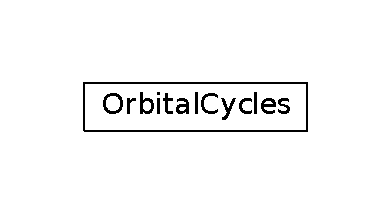
\includegraphics{inheritance-d20a99af4787ada459f19081acae8208cc46265a.pdf}
\phantomsection\label{api/climlab.solar:module-climlab.solar.orbital_cycles}\index{climlab.solar.orbital\_cycles (module)}\index{OrbitalCycles (class in climlab.solar.orbital\_cycles)}

\begin{fulllineitems}
\phantomsection\label{api/climlab.solar:climlab.solar.orbital_cycles.OrbitalCycles}\pysiglinewithargsret{\strong{class }\code{climlab.solar.orbital\_cycles.}\bfcode{OrbitalCycles}}{\emph{model}, \emph{kyear\_start=-20.0}, \emph{kyear\_stop=0.0}, \emph{segment\_length\_years=100.0}, \emph{orbital\_year\_factor=1.0}, \emph{verbose=True}}{}
Automatically integrates a process through changes in orbital parameters.

OrbitalCycles is a module for setting up long integrations of climlab 
processes over orbital cycles.

The duration between integration start and end time is partitioned in 
time segments over which the orbital parameters are held constant.
The process is integrated over every time segment and the process state
\code{Ts} is stored for each segment.

The storage arrays are saving:
\begin{itemize}
\item {} 
\textbf{current model state} at end of each segment

\item {} 
\textbf{model state averaged} over last integrated year of each segment

\item {} 
\textbf{global mean} of averaged model state over last integrated year 
of each segment

\end{itemize}

\begin{notice}{note}{Note:}
Input \code{kyear} is thousands of years after present.
For years before present, use \code{kyear \textless{} 0}.
\end{notice}

\textbf{Initialization parameters}
\begin{quote}\begin{description}
\item[{Parameters}] \leavevmode\begin{itemize}
\item {} 
\textbf{\texttt{model}} ({\hyperref[api/climlab.process:climlab.process.time_dependent_process.TimeDependentProcess]{\emph{\code{TimeDependentProcess}}}} (\autopageref*{api/climlab.process:climlab.process.time_dependent_process.TimeDependentProcess})) -- a time dependent process

\item {} 
\textbf{\texttt{kyear\_start}} (\href{http://docs.python.org/2.7/library/functions.html\#float}{\emph{\texttt{float}}}) -- 
integration start time.

As time reference
is present, argument should be \(<0\) 
for time before present.
\begin{itemize}
\item {} 
\emph{unit:} kiloyears

\item {} 
\emph{default value:} \code{-20.}

\end{itemize}


\item {} 
\textbf{\texttt{kyear\_stop}} (\href{http://docs.python.org/2.7/library/functions.html\#float}{\emph{\texttt{float}}}) -- 
integration stop time.

As time reference
is present, argument should be \(\le 0\) 
for time before present.
\begin{itemize}
\item {} 
\emph{unit:} kiloyears

\item {} 
\emph{default value:} \code{0.}

\end{itemize}


\item {} 
\textbf{\texttt{segment\_length\_years}} (\href{http://docs.python.org/2.7/library/functions.html\#float}{\emph{\texttt{float}}}) -- is the length of each integration with
fixed orbital parameters. {[}default: 100.{]}

\item {} 
\textbf{\texttt{orbital\_year\_factor}} (\href{http://docs.python.org/2.7/library/functions.html\#float}{\emph{\texttt{float}}}) -- is an optional speed-up to the orbital cycles.
{[}default: 1.{]}

\item {} 
\textbf{\texttt{verbose}} (\href{http://docs.python.org/2.7/library/functions.html\#bool}{\emph{\texttt{bool}}}) -- prints product of calculation and
information about computation progress
{[}default: True{]}

\end{itemize}

\end{description}\end{quote}

\textbf{Object attributes}

Following object attributes are generated during initialization:
\begin{quote}\begin{description}
\item[{Variables}] \leavevmode\begin{itemize}
\item {} 
\textbf{\texttt{model}} ({\hyperref[api/climlab.process:climlab.process.time_dependent_process.TimeDependentProcess]{\emph{\code{TimeDependentProcess}}}} (\autopageref*{api/climlab.process:climlab.process.time_dependent_process.TimeDependentProcess})) -- timedependent process to be integrated

\item {} 
\textbf{\texttt{kyear\_start}} (\href{http://docs.python.org/2.7/library/functions.html\#float}{\emph{\texttt{float}}}) -- integration start time

\item {} 
\textbf{\texttt{kyear\_stop}} (\href{http://docs.python.org/2.7/library/functions.html\#float}{\emph{\texttt{float}}}) -- integration stop time

\item {} 
\textbf{\texttt{segment\_length\_years}} (\href{http://docs.python.org/2.7/library/functions.html\#float}{\emph{\texttt{float}}}) -- length of each integration with
fixed orbital parameters

\item {} 
\textbf{\texttt{orbital\_year\_factor}} (\href{http://docs.python.org/2.7/library/functions.html\#float}{\emph{\texttt{float}}}) -- speed-up factor  to the orbital cycles

\item {} 
\textbf{\texttt{verbose}} (\href{http://docs.python.org/2.7/library/functions.html\#bool}{\emph{\texttt{bool}}}) -- print flag

\item {} 
\textbf{\texttt{num\_segments}} (\href{http://docs.python.org/2.7/library/functions.html\#int}{\emph{\texttt{int}}}) -- 
number of segments with fixed oribtal 
parameters, calculated through:
\begin{gather}
\begin{split}num_{seg} = \frac{-(kyear_{start}-kyear_{stop})*1000}{seg_{length} * orb_{factor}}\end{split}\notag
\end{gather}

\item {} 
\textbf{\texttt{T\_segments\_global}} (\href{http://docs.python.org/2.7/library/array.html\#module-array}{\emph{\texttt{array}}}) -- storage for global mean temperature
for final year of each segment

\item {} 
\textbf{\texttt{T\_segments}} (\href{http://docs.python.org/2.7/library/array.html\#module-array}{\emph{\texttt{array}}}) -- storage for actual temperature at end
of each segment

\item {} 
\textbf{\texttt{T\_segments\_annual}} (\href{http://docs.python.org/2.7/library/array.html\#module-array}{\emph{\texttt{array}}}) -- 
storage for timeaveraged temperature 
over last year of segment

dimension: (size(Ts), num\_segments)


\item {} 
\textbf{\texttt{orb\_kyear}} (\href{http://docs.python.org/2.7/library/array.html\#module-array}{\emph{\texttt{array}}}) -- integration start time of all segments

\item {} 
{\hyperref[api/climlab.radiation:climlab.radiation.insolation.AnnualMeanInsolation.orb]{\emph{\textbf{\texttt{orb}}}}} (\autopageref*{api/climlab.radiation:climlab.radiation.insolation.AnnualMeanInsolation.orb}) (\href{http://docs.python.org/2.7/library/stdtypes.html\#dict}{\emph{\texttt{dict}}}) -- orbital parameters for last integrated segment

\end{itemize}

\item[{Example}] \leavevmode
Integration of an energy balance model for 10,000 years with 
corresponding orbital parameters:

\begin{Verbatim}[commandchars=\\\{\}]
\PYG{k+kn}{from} \PYG{n+nn}{climlab.model.ebm} \PYG{k+kn}{import} \PYG{n}{EBM\PYGZus{}seasonal}
\PYG{k+kn}{from} \PYG{n+nn}{climlab.solar.orbital\PYGZus{}cycles} \PYG{k+kn}{import} \PYG{n}{OrbitalCycles}
\PYG{k+kn}{from} \PYG{n+nn}{climlab.surface.albedo} \PYG{k+kn}{import} \PYG{n}{StepFunctionAlbedo}
\PYG{n}{ebm} \PYG{o}{=} \PYG{n}{EBM\PYGZus{}seasonal}\PYG{p}{(}\PYG{p}{)}
\PYG{k}{print} \PYG{n}{ebm}

\PYG{c+c1}{\PYGZsh{}  add an albedo feedback}
\PYG{n}{albedo} \PYG{o}{=} \PYG{n}{StepFunctionAlbedo}\PYG{p}{(}\PYG{n}{state}\PYG{o}{=}\PYG{n}{ebm}\PYG{o}{.}\PYG{n}{state}\PYG{p}{,} \PYG{o}{*}\PYG{o}{*}\PYG{n}{ebm}\PYG{o}{.}\PYG{n}{param}\PYG{p}{)}
\PYG{n}{ebm}\PYG{o}{.}\PYG{n}{add\PYGZus{}subprocess}\PYG{p}{(}\PYG{l+s+s1}{\PYGZsq{}}\PYG{l+s+s1}{albedo}\PYG{l+s+s1}{\PYGZsq{}}\PYG{p}{,} \PYG{n}{albedo}\PYG{p}{)}

\PYG{c+c1}{\PYGZsh{}  start the integration}
\PYG{c+c1}{\PYGZsh{}  run for 10,000 orbital years, but only 1,000 model years}
\PYG{n}{experiment} \PYG{o}{=} \PYG{n}{OrbitalCycles}\PYG{p}{(}\PYG{n}{ebm}\PYG{p}{,} \PYG{n}{kyear\PYGZus{}start}\PYG{o}{=}\PYG{o}{\PYGZhy{}}\PYG{l+m+mi}{20}\PYG{p}{,} \PYG{n}{kyear\PYGZus{}stop}\PYG{o}{=}\PYG{o}{\PYGZhy{}}\PYG{l+m+mi}{10}\PYG{p}{,}                                                         \PYG{n}{orbital\PYGZus{}year\PYGZus{}factor}\PYG{o}{=}\PYG{l+m+mf}{10.}\PYG{p}{)}
\end{Verbatim}

\end{description}\end{quote}

\end{fulllineitems}



\subsection{climlab.surface package}
\label{api/climlab.surface:climlab-surface-package}\label{api/climlab.surface::doc}

\subsubsection{climlab.surface.albedo module}
\label{api/climlab.surface:climlab-surface-albedo-module}
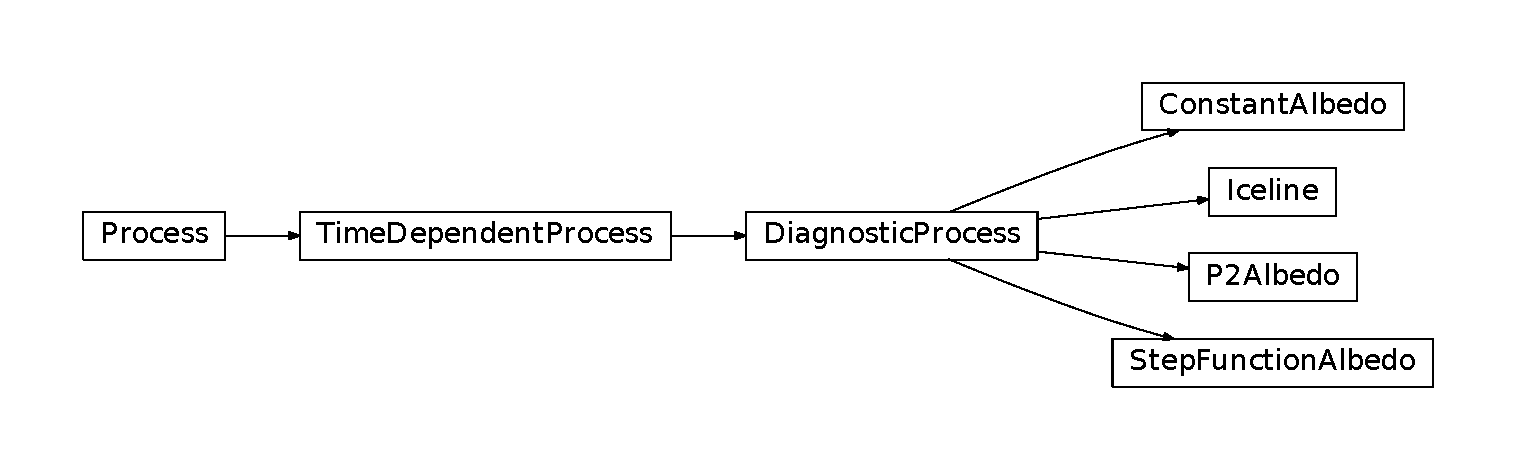
\includegraphics{inheritance-742cd8325d5c78229cd3bff3a540d679a72c377c.pdf}
\phantomsection\label{api/climlab.surface:module-climlab.surface.albedo}\index{climlab.surface.albedo (module)}\index{ConstantAlbedo (class in climlab.surface.albedo)}

\begin{fulllineitems}
\phantomsection\label{api/climlab.surface:climlab.surface.albedo.ConstantAlbedo}\pysiglinewithargsret{\strong{class }\code{climlab.surface.albedo.}\bfcode{ConstantAlbedo}}{\emph{albedo=0.33}, \emph{**kwargs}}{}
Bases: {\hyperref[api/climlab.process:climlab.process.diagnostic.DiagnosticProcess]{\emph{\code{climlab.process.diagnostic.DiagnosticProcess}}}} (\autopageref*{api/climlab.process:climlab.process.diagnostic.DiagnosticProcess})

A class for constant albedo values at all spatial points of the domain.

\textbf{Initialization parameters}
\begin{quote}\begin{description}
\item[{Parameters}] \leavevmode
\textbf{\texttt{albedo}} (\href{http://docs.python.org/2.7/library/functions.html\#float}{\emph{\texttt{float}}}) -- albedo values {[}default: 0.33{]}

\end{description}\end{quote}

\textbf{Object attributes}

Additional to the parent class 
{\hyperref[api/climlab.process:climlab.process.diagnostic.DiagnosticProcess]{\emph{\code{DiagnosticProcess}}}} (\autopageref*{api/climlab.process:climlab.process.diagnostic.DiagnosticProcess})
following object attributes are generated and updated during initialization:
\begin{quote}\begin{description}
\item[{Variables}] \leavevmode
{\hyperref[api/climlab.surface:climlab.surface.albedo.P2Albedo.albedo]{\emph{\textbf{\texttt{albedo}}}}} (\autopageref*{api/climlab.surface:climlab.surface.albedo.P2Albedo.albedo}) ({\hyperref[api/climlab.domain:climlab.domain.field.Field]{\emph{\emph{\texttt{Field}}}}} (\autopageref*{api/climlab.domain:climlab.domain.field.Field})) -- attribute to store the albedo value. 
During initialization the 
{\hyperref[api/climlab.surface:climlab.surface.albedo.ConstantAlbedo.albedo]{\emph{\code{albedo()}}}} (\autopageref*{api/climlab.surface:climlab.surface.albedo.ConstantAlbedo.albedo}) setter is called.

\item[{Example}] \leavevmode
Creation of a constant albedo subprocess on basis of an EBM domain:

\begin{Verbatim}[commandchars=\\\{\}]
\PYG{g+gp}{\PYGZgt{}\PYGZgt{}\PYGZgt{} }\PYG{k+kn}{import} \PYG{n+nn}{climlab}
\PYG{g+gp}{\PYGZgt{}\PYGZgt{}\PYGZgt{} }\PYG{k+kn}{from} \PYG{n+nn}{climlab.surface.albedo} \PYG{k+kn}{import} \PYG{n}{ConstantAlbedo}

\PYG{g+gp}{\PYGZgt{}\PYGZgt{}\PYGZgt{} }\PYG{c+c1}{\PYGZsh{} model creation}
\PYG{g+gp}{\PYGZgt{}\PYGZgt{}\PYGZgt{} }\PYG{n}{model} \PYG{o}{=} \PYG{n}{climlab}\PYG{o}{.}\PYG{n}{EBM}\PYG{p}{(}\PYG{p}{)}

\PYG{g+gp}{\PYGZgt{}\PYGZgt{}\PYGZgt{} }\PYG{n}{sfc} \PYG{o}{=} \PYG{n}{model}\PYG{o}{.}\PYG{n}{domains}\PYG{p}{[}\PYG{l+s+s1}{\PYGZsq{}}\PYG{l+s+s1}{Ts}\PYG{l+s+s1}{\PYGZsq{}}\PYG{p}{]}            

\PYG{g+gp}{\PYGZgt{}\PYGZgt{}\PYGZgt{} }\PYG{c+c1}{\PYGZsh{} subprocess creation}
\PYG{g+gp}{\PYGZgt{}\PYGZgt{}\PYGZgt{} }\PYG{n}{const\PYGZus{}alb} \PYG{o}{=} \PYG{n}{ConstantAlbedo}\PYG{p}{(}\PYG{n}{albedo}\PYG{o}{=}\PYG{l+m+mf}{0.3}\PYG{p}{,} \PYG{n}{domains}\PYG{o}{=}\PYG{n}{sfc}\PYG{p}{,} \PYG{o}{*}\PYG{o}{*}\PYG{n}{model}\PYG{o}{.}\PYG{n}{param}\PYG{p}{)}
\end{Verbatim}

\end{description}\end{quote}

Uniform prescribed albedo.
\index{albedo (climlab.surface.albedo.ConstantAlbedo attribute)}

\begin{fulllineitems}
\phantomsection\label{api/climlab.surface:climlab.surface.albedo.ConstantAlbedo.albedo}\pysigline{\bfcode{albedo}}
Property of albedo value.
\begin{quote}\begin{description}
\item[{Getter}] \leavevmode
Returns the albedo value which is stored in diagnostic dict 
\code{self.diagnostic{[}'albedo'{]}}

\item[{Setter}] \leavevmode\begin{itemize}
\item {} 
sets albedo which is addressed as \code{diagnostics{[}'albedo'{]}} 
to the new value through creating a Field on the basis 
of domain \code{self.domain{[}'default'{]}}

\item {} 
updates the parameter dictionary \code{self.param{[}'albedo'{]}}

\end{itemize}

\item[{Type}] \leavevmode
Field

\end{description}\end{quote}

\end{fulllineitems}


\end{fulllineitems}

\index{Iceline (class in climlab.surface.albedo)}

\begin{fulllineitems}
\phantomsection\label{api/climlab.surface:climlab.surface.albedo.Iceline}\pysiglinewithargsret{\strong{class }\code{climlab.surface.albedo.}\bfcode{Iceline}}{\emph{Tf=-10.0}, \emph{**kwargs}}{}
Bases: {\hyperref[api/climlab.process:climlab.process.diagnostic.DiagnosticProcess]{\emph{\code{climlab.process.diagnostic.DiagnosticProcess}}}} (\autopageref*{api/climlab.process:climlab.process.diagnostic.DiagnosticProcess})

A class for an Iceline subprocess.

Depending on a freezing temperature it calculates where on the domain the
surface is covered with ice, where there is no ice and on which latitude the ice-edge 
is placed.

\textbf{Initialization parameters}
\begin{quote}\begin{description}
\item[{Parameters}] \leavevmode
\textbf{\texttt{Tf}} (\href{http://docs.python.org/2.7/library/functions.html\#float}{\emph{\texttt{float}}}) -- 
freezing temperature where sea water freezes and
surface is covered with ice
\begin{itemize}
\item {} 
unit: \(^{\circ} \textrm{C}\)

\item {} 
default value: \code{-10}

\end{itemize}


\end{description}\end{quote}

\textbf{Object attributes}

Additional to the parent class 
{\hyperref[api/climlab.process:climlab.process.diagnostic.DiagnosticProcess]{\emph{\code{DiagnosticProcess}}}} (\autopageref*{api/climlab.process:climlab.process.diagnostic.DiagnosticProcess})
following object attributes are generated and updated during initialization:
\begin{quote}\begin{description}
\item[{Variables}] \leavevmode\begin{itemize}
\item {} 
\textbf{\texttt{param}} (\href{http://docs.python.org/2.7/library/stdtypes.html\#dict}{\emph{\texttt{dict}}}) -- The parameter dictionary is updated with the 
input argument \code{'Tf'}.

\item {} 
\textbf{\texttt{diagnostics}} (\href{http://docs.python.org/2.7/library/stdtypes.html\#dict}{\emph{\texttt{dict}}}) -- key \code{'icelat'} initialized

\item {} 
{\hyperref[api/climlab.surface:climlab.surface.albedo.Iceline.icelat]{\emph{\textbf{\texttt{icelat}}}}} (\autopageref*{api/climlab.surface:climlab.surface.albedo.Iceline.icelat}) (\href{http://docs.python.org/2.7/library/array.html\#module-array}{\emph{\texttt{array}}}) -- the subprocess attribute \code{self.icelat} is
created

\end{itemize}

\end{description}\end{quote}
\index{find\_icelines() (climlab.surface.albedo.Iceline method)}

\begin{fulllineitems}
\phantomsection\label{api/climlab.surface:climlab.surface.albedo.Iceline.find_icelines}\pysiglinewithargsret{\bfcode{find\_icelines}}{}{}
Finds iceline according to the surface temperature.

This method is called by the private function 
\code{\_compute()}
and updates following attributes according to the freezing temperature
\code{self.param{[}'Tf'{]}} and the surface temperature \code{self.param{[}'Ts'{]}}:

\textbf{Object attributes}
\begin{quote}\begin{description}
\item[{Variables}] \leavevmode\begin{itemize}
\item {} 
\textbf{\texttt{noice}} ({\hyperref[api/climlab.domain:climlab.domain.field.Field]{\emph{\emph{\texttt{Field}}}}} (\autopageref*{api/climlab.domain:climlab.domain.field.Field})) -- a Field of booleans which are \code{True} where
\(T_s \ge T_f\)

\item {} 
\textbf{\texttt{ice}} ({\hyperref[api/climlab.domain:climlab.domain.field.Field]{\emph{\emph{\texttt{Field}}}}} (\autopageref*{api/climlab.domain:climlab.domain.field.Field})) -- a Field of booleans which are \code{True} where
\(T_s < T_f\)

\item {} 
{\hyperref[api/climlab.surface:climlab.surface.albedo.Iceline.icelat]{\emph{\textbf{\texttt{icelat}}}}} (\autopageref*{api/climlab.surface:climlab.surface.albedo.Iceline.icelat}) (\href{http://docs.python.org/2.7/library/array.html\#module-array}{\emph{\texttt{array}}}) -- an array with two elements indicating the 
ice-edge latitudes

\item {} 
\textbf{\texttt{diagnostics}} (\href{http://docs.python.org/2.7/library/stdtypes.html\#dict}{\emph{\texttt{dict}}}) -- key \code{'icelat'} is updated according to object
attribute \code{self.icelat} during modification

\end{itemize}

\end{description}\end{quote}

\end{fulllineitems}

\index{icelat (climlab.surface.albedo.Iceline attribute)}

\begin{fulllineitems}
\phantomsection\label{api/climlab.surface:climlab.surface.albedo.Iceline.icelat}\pysigline{\bfcode{icelat}}
\end{fulllineitems}


\end{fulllineitems}

\index{P2Albedo (class in climlab.surface.albedo)}

\begin{fulllineitems}
\phantomsection\label{api/climlab.surface:climlab.surface.albedo.P2Albedo}\pysiglinewithargsret{\strong{class }\code{climlab.surface.albedo.}\bfcode{P2Albedo}}{\emph{a0=0.33}, \emph{a2=0.25}, \emph{**kwargs}}{}
Bases: {\hyperref[api/climlab.process:climlab.process.diagnostic.DiagnosticProcess]{\emph{\code{climlab.process.diagnostic.DiagnosticProcess}}}} (\autopageref*{api/climlab.process:climlab.process.diagnostic.DiagnosticProcess})

A class for parabolic distributed albedo values across the domain 
on basis of the second order Legendre Polynomial.

Calculates the latitude dependent albedo values as
\begin{gather}
\begin{split}\alpha(\varphi) = a_0 + a_2 P_2(x)\end{split}\notag
\end{gather}
where \(P_2(x) = \frac{1}{2} (3x^2 - 1)\) is the second order Legendre Polynomial
and \(x=sin(\varphi)\).

\textbf{Initialization parameters}
\begin{quote}\begin{description}
\item[{Parameters}] \leavevmode\begin{itemize}
\item {} 
\textbf{\texttt{a0}} (\href{http://docs.python.org/2.7/library/functions.html\#float}{\emph{\texttt{float}}}) -- basic parameter for albedo function {[}default: 0.33{]}

\item {} 
\textbf{\texttt{a2}} (\href{http://docs.python.org/2.7/library/functions.html\#float}{\emph{\texttt{float}}}) -- factor for second legendre polynominal term in albedo 
function {[}default: 0.25{]}

\end{itemize}

\end{description}\end{quote}

\textbf{Object attributes}

Additional to the parent class 
{\hyperref[api/climlab.process:climlab.process.diagnostic.DiagnosticProcess]{\emph{\code{DiagnosticProcess}}}} (\autopageref*{api/climlab.process:climlab.process.diagnostic.DiagnosticProcess})
following object attributes are generated and updated during initialization:
\begin{quote}\begin{description}
\item[{Variables}] \leavevmode\begin{itemize}
\item {} 
{\hyperref[api/climlab.surface:climlab.surface.albedo.P2Albedo.a0]{\emph{\textbf{\texttt{a0}}}}} (\autopageref*{api/climlab.surface:climlab.surface.albedo.P2Albedo.a0}) (\href{http://docs.python.org/2.7/library/functions.html\#float}{\emph{\texttt{float}}}) -- attribute to store the albedo parameter a0. 
During initialization the 
{\hyperref[api/climlab.surface:climlab.surface.albedo.P2Albedo.a0]{\emph{\code{a0()}}}} (\autopageref*{api/climlab.surface:climlab.surface.albedo.P2Albedo.a0}) setter is called.

\item {} 
{\hyperref[api/climlab.surface:climlab.surface.albedo.P2Albedo.a2]{\emph{\textbf{\texttt{a2}}}}} (\autopageref*{api/climlab.surface:climlab.surface.albedo.P2Albedo.a2}) (\href{http://docs.python.org/2.7/library/functions.html\#float}{\emph{\texttt{float}}}) -- attribute to store the albedo parameter a2. 
During initialization the 
{\hyperref[api/climlab.surface:climlab.surface.albedo.P2Albedo.a2]{\emph{\code{a2()}}}} (\autopageref*{api/climlab.surface:climlab.surface.albedo.P2Albedo.a2}) setter is called.

\item {} 
\textbf{\texttt{diagnostics}} (\href{http://docs.python.org/2.7/library/stdtypes.html\#dict}{\emph{\texttt{dict}}}) -- key \code{'albedo'} initialized

\item {} 
{\hyperref[api/climlab.surface:climlab.surface.albedo.P2Albedo.albedo]{\emph{\textbf{\texttt{albedo}}}}} (\autopageref*{api/climlab.surface:climlab.surface.albedo.P2Albedo.albedo}) ({\hyperref[api/climlab.domain:climlab.domain.field.Field]{\emph{\emph{\texttt{Field}}}}} (\autopageref*{api/climlab.domain:climlab.domain.field.Field})) -- the subprocess attribute \code{self.albedo} is
created with correct dimensions 
(according to \code{self.lat})

\end{itemize}

\item[{Example}] \leavevmode
Creation of a parabolic albedo subprocess on basis of an EBM domain:

\begin{Verbatim}[commandchars=\\\{\}]
\PYG{g+gp}{\PYGZgt{}\PYGZgt{}\PYGZgt{} }\PYG{k+kn}{import} \PYG{n+nn}{climlab}
\PYG{g+gp}{\PYGZgt{}\PYGZgt{}\PYGZgt{} }\PYG{k+kn}{from} \PYG{n+nn}{climlab.surface.albedo} \PYG{k+kn}{import} \PYG{n}{P2Albedo}

\PYG{g+gp}{\PYGZgt{}\PYGZgt{}\PYGZgt{} }\PYG{c+c1}{\PYGZsh{} model creation}
\PYG{g+gp}{\PYGZgt{}\PYGZgt{}\PYGZgt{} }\PYG{n}{model} \PYG{o}{=} \PYG{n}{climlab}\PYG{o}{.}\PYG{n}{EBM}\PYG{p}{(}\PYG{p}{)}

\PYG{g+gp}{\PYGZgt{}\PYGZgt{}\PYGZgt{} }\PYG{c+c1}{\PYGZsh{} modify a0 and a2 values in model parameter dictionary}
\PYG{g+gp}{\PYGZgt{}\PYGZgt{}\PYGZgt{} }\PYG{n}{model}\PYG{o}{.}\PYG{n}{param}\PYG{p}{[}\PYG{l+s+s1}{\PYGZsq{}}\PYG{l+s+s1}{a0}\PYG{l+s+s1}{\PYGZsq{}}\PYG{p}{]}\PYG{o}{=}\PYG{l+m+mf}{0.35}
\PYG{g+gp}{\PYGZgt{}\PYGZgt{}\PYGZgt{} }\PYG{n}{model}\PYG{o}{.}\PYG{n}{param}\PYG{p}{[}\PYG{l+s+s1}{\PYGZsq{}}\PYG{l+s+s1}{a2}\PYG{l+s+s1}{\PYGZsq{}}\PYG{p}{]}\PYG{o}{=} \PYG{l+m+mf}{0.10}

\PYG{g+gp}{\PYGZgt{}\PYGZgt{}\PYGZgt{} }\PYG{c+c1}{\PYGZsh{} subprocess creation}
\PYG{g+gp}{\PYGZgt{}\PYGZgt{}\PYGZgt{} }\PYG{n}{p2\PYGZus{}alb} \PYG{o}{=} \PYG{n}{P2Albedo}\PYG{p}{(}\PYG{n}{domains}\PYG{o}{=}\PYG{n}{model}\PYG{o}{.}\PYG{n}{domains}\PYG{p}{[}\PYG{l+s+s1}{\PYGZsq{}}\PYG{l+s+s1}{Ts}\PYG{l+s+s1}{\PYGZsq{}}\PYG{p}{]}\PYG{p}{,} \PYG{o}{*}\PYG{o}{*}\PYG{n}{model}\PYG{o}{.}\PYG{n}{param}\PYG{p}{)}

\PYG{g+gp}{\PYGZgt{}\PYGZgt{}\PYGZgt{} }\PYG{n}{p2\PYGZus{}alb}\PYG{o}{.}\PYG{n}{a0}
\PYG{g+go}{0.33}
\PYG{g+gp}{\PYGZgt{}\PYGZgt{}\PYGZgt{} }\PYG{n}{p2\PYGZus{}alb}\PYG{o}{.}\PYG{n}{a2}
\PYG{g+go}{0.1}
\end{Verbatim}

\end{description}\end{quote}
\index{a0 (climlab.surface.albedo.P2Albedo attribute)}

\begin{fulllineitems}
\phantomsection\label{api/climlab.surface:climlab.surface.albedo.P2Albedo.a0}\pysigline{\bfcode{a0}}
Property of albedo parameter a0.
\begin{quote}\begin{description}
\item[{Getter}] \leavevmode
Returns the albedo parameter value which is stored in attribute 
\code{self.\_a0}

\item[{Setter}] \leavevmode\begin{itemize}
\item {} 
sets albedo parameter which is addressed as \code{self.\_a0} 
to the new value

\item {} 
updates the parameter dictionary \code{self.param{[}'a0'{]}}

\item {} 
calls method \code{\_compute\_fixed()}

\end{itemize}

\item[{Type}] \leavevmode
float

\end{description}\end{quote}

\end{fulllineitems}

\index{a2 (climlab.surface.albedo.P2Albedo attribute)}

\begin{fulllineitems}
\phantomsection\label{api/climlab.surface:climlab.surface.albedo.P2Albedo.a2}\pysigline{\bfcode{a2}}
Property of albedo parameter a2.
\begin{quote}\begin{description}
\item[{Getter}] \leavevmode
Returns the albedo parameter value which is stored in attribute 
\code{self.\_a2}

\item[{Setter}] \leavevmode\begin{itemize}
\item {} 
sets albedo parameter which is addressed as \code{self.\_a2} 
to the new value

\item {} 
updates the parameter dictionary \code{self.param{[}'a2'{]}}

\item {} 
calls method \code{\_compute\_fixed()}

\end{itemize}

\item[{Type}] \leavevmode
float

\end{description}\end{quote}

\end{fulllineitems}

\index{albedo (climlab.surface.albedo.P2Albedo attribute)}

\begin{fulllineitems}
\phantomsection\label{api/climlab.surface:climlab.surface.albedo.P2Albedo.albedo}\pysigline{\bfcode{albedo}}
\end{fulllineitems}


\end{fulllineitems}

\index{StepFunctionAlbedo (class in climlab.surface.albedo)}

\begin{fulllineitems}
\phantomsection\label{api/climlab.surface:climlab.surface.albedo.StepFunctionAlbedo}\pysiglinewithargsret{\strong{class }\code{climlab.surface.albedo.}\bfcode{StepFunctionAlbedo}}{\emph{Tf=-10.0}, \emph{a0=0.3}, \emph{a2=0.078}, \emph{ai=0.62}, \emph{**kwargs}}{}
Bases: {\hyperref[api/climlab.process:climlab.process.diagnostic.DiagnosticProcess]{\emph{\code{climlab.process.diagnostic.DiagnosticProcess}}}} (\autopageref*{api/climlab.process:climlab.process.diagnostic.DiagnosticProcess})

A step function albedo suprocess.

This class itself defines three subprocesses that are created during 
initialization:
\begin{itemize}
\item {} 
\code{'iceline'} - {\hyperref[api/climlab.surface:climlab.surface.albedo.Iceline]{\emph{\code{Iceline}}}} (\autopageref*{api/climlab.surface:climlab.surface.albedo.Iceline})

\item {} 
\code{'warm\_albedo'} - {\hyperref[api/climlab.surface:climlab.surface.albedo.P2Albedo]{\emph{\code{P2Albedo}}}} (\autopageref*{api/climlab.surface:climlab.surface.albedo.P2Albedo})

\item {} 
\code{'cold\_albedo'} - {\hyperref[api/climlab.surface:climlab.surface.albedo.ConstantAlbedo]{\emph{\code{ConstantAlbedo}}}} (\autopageref*{api/climlab.surface:climlab.surface.albedo.ConstantAlbedo})

\end{itemize}

\textbf{Initialization parameters}
\begin{quote}\begin{description}
\item[{Parameters}] \leavevmode\begin{itemize}
\item {} 
\textbf{\texttt{Tf}} (\href{http://docs.python.org/2.7/library/functions.html\#float}{\emph{\texttt{float}}}) -- 
freezing temperature for Iceline subprocess
\begin{itemize}
\item {} 
unit: \(^{\circ} \textrm{C}\)

\item {} 
default value: \code{-10}

\end{itemize}


\item {} 
\textbf{\texttt{a0}} (\href{http://docs.python.org/2.7/library/functions.html\#float}{\emph{\texttt{float}}}) -- basic parameter for P2Albedo subprocess {[}default: 0.3{]}

\item {} 
\textbf{\texttt{a2}} (\href{http://docs.python.org/2.7/library/functions.html\#float}{\emph{\texttt{float}}}) -- factor for second legendre polynominal term in P2Albedo
subprocess {[}default: 0.078{]}

\item {} 
\textbf{\texttt{ai}} (\href{http://docs.python.org/2.7/library/functions.html\#float}{\emph{\texttt{float}}}) -- ice albedo value for ConstantAlbedo subprocess
{[}default: 0.62{]}

\end{itemize}

\end{description}\end{quote}

Additional to the parent class 
{\hyperref[api/climlab.process:climlab.process.diagnostic.DiagnosticProcess]{\emph{\code{DiagnosticProcess}}}} (\autopageref*{api/climlab.process:climlab.process.diagnostic.DiagnosticProcess})
following object attributes are generated/updated during initialization:
\begin{quote}\begin{description}
\item[{Variables}] \leavevmode\begin{itemize}
\item {} 
\textbf{\texttt{param}} (\href{http://docs.python.org/2.7/library/stdtypes.html\#dict}{\emph{\texttt{dict}}}) -- The parameter dictionary is updated with 
a couple of the initatilzation input 
arguments, namely \code{'Tf'}, \code{'a0'}, 
\code{'a2'} and \code{'ai'}.

\item {} 
\textbf{\texttt{topdown}} (\href{http://docs.python.org/2.7/library/functions.html\#bool}{\emph{\texttt{bool}}}) -- is set to \code{False} to call subprocess
compute method first

\item {} 
\textbf{\texttt{diagnostics}} (\href{http://docs.python.org/2.7/library/stdtypes.html\#dict}{\emph{\texttt{dict}}}) -- key \code{'albedo'} initialized

\item {} 
{\hyperref[api/climlab.surface:climlab.surface.albedo.P2Albedo.albedo]{\emph{\textbf{\texttt{albedo}}}}} (\autopageref*{api/climlab.surface:climlab.surface.albedo.P2Albedo.albedo}) ({\hyperref[api/climlab.domain:climlab.domain.field.Field]{\emph{\emph{\texttt{Field}}}}} (\autopageref*{api/climlab.domain:climlab.domain.field.Field})) -- the subprocess attribute \code{self.albedo} is
created

\end{itemize}

\item[{Example}] \leavevmode
Creation of a step albedo subprocess on basis of an EBM domain:

\begin{Verbatim}[commandchars=\\\{\}]
\PYG{g+gp}{\PYGZgt{}\PYGZgt{}\PYGZgt{} }\PYG{k+kn}{import} \PYG{n+nn}{climlab}
\PYG{g+gp}{\PYGZgt{}\PYGZgt{}\PYGZgt{} }\PYG{k+kn}{from} \PYG{n+nn}{climlab.surface.albedo} \PYG{k+kn}{import} \PYG{n}{StepFunctionAlbedo}
\PYG{g+gp}{\PYGZgt{}\PYGZgt{}\PYGZgt{} }
\PYG{g+gp}{\PYGZgt{}\PYGZgt{}\PYGZgt{} }\PYG{n}{model} \PYG{o}{=} \PYG{n}{climlab}\PYG{o}{.}\PYG{n}{EBM}\PYG{p}{(}\PYG{n}{a0}\PYG{o}{=}\PYG{l+m+mf}{0.29}\PYG{p}{,} \PYG{n}{a2}\PYG{o}{=}\PYG{l+m+mf}{0.1}\PYG{p}{,} \PYG{n}{ai}\PYG{o}{=}\PYG{l+m+mf}{0.65}\PYG{p}{,} \PYG{n}{Tf}\PYG{o}{=}\PYG{o}{\PYGZhy{}}\PYG{l+m+mi}{2}\PYG{p}{)}
\PYG{g+gp}{\PYGZgt{}\PYGZgt{}\PYGZgt{} }
\PYG{g+gp}{\PYGZgt{}\PYGZgt{}\PYGZgt{} }\PYG{n}{step\PYGZus{}alb} \PYG{o}{=} \PYG{n}{StepFunctionAlbedo}\PYG{p}{(}\PYG{n}{state}\PYG{o}{=} \PYG{n}{model}\PYG{o}{.}\PYG{n}{state}\PYG{p}{,} \PYG{o}{*}\PYG{o}{*}\PYG{n}{model}\PYG{o}{.}\PYG{n}{param}\PYG{p}{)}
\PYG{g+gp}{\PYGZgt{}\PYGZgt{}\PYGZgt{} }
\PYG{g+gp}{\PYGZgt{}\PYGZgt{}\PYGZgt{} }\PYG{k}{print} \PYG{n}{step\PYGZus{}alb}
\PYG{g+go}{climlab Process of type \PYGZlt{}class \PYGZsq{}climlab.surface.albedo.StepFunctionAlbedo\PYGZsq{}\PYGZgt{}. }
\PYG{g+go}{State variables and domain shapes: }
\PYG{g+go}{  Ts: (90, 1) }
\PYG{g+go}{The subprocess tree: }
\PYG{g+go}{top: \PYGZlt{}class \PYGZsq{}climlab.surface.albedo.StepFunctionAlbedo\PYGZsq{}\PYGZgt{}}
\PYG{g+go}{   iceline: \PYGZlt{}class \PYGZsq{}climlab.surface.albedo.Iceline\PYGZsq{}\PYGZgt{}}
\PYG{g+go}{   cold\PYGZus{}albedo: \PYGZlt{}class \PYGZsq{}climlab.surface.albedo.ConstantAlbedo\PYGZsq{}\PYGZgt{}}
\PYG{g+go}{   warm\PYGZus{}albedo: \PYGZlt{}class \PYGZsq{}climlab.surface.albedo.P2Albedo\PYGZsq{}\PYGZgt{}}
\end{Verbatim}

\end{description}\end{quote}
\index{albedo (climlab.surface.albedo.StepFunctionAlbedo attribute)}

\begin{fulllineitems}
\phantomsection\label{api/climlab.surface:climlab.surface.albedo.StepFunctionAlbedo.albedo}\pysigline{\bfcode{albedo}}
\end{fulllineitems}


\end{fulllineitems}



\subsection{climlab.utils package}
\label{api/climlab.utils::doc}\label{api/climlab.utils:climlab-utils-package}

\subsubsection{climlab.utils.attr\_dict module}
\label{api/climlab.utils:climlab-utils-attr-dict-module}
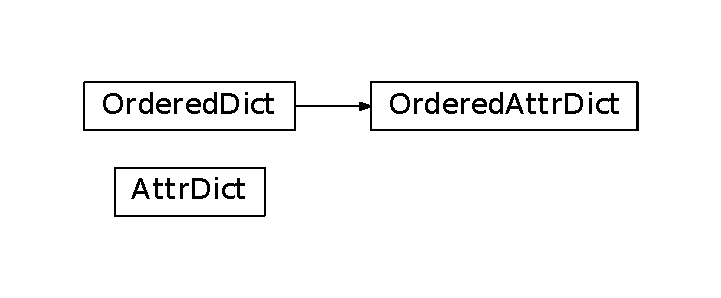
\includegraphics{inheritance-bef65cee25121f0f467c31bf205dd368e8cec68f.pdf}
\phantomsection\label{api/climlab.utils:module-climlab.utils.attr_dict}\index{climlab.utils.attr\_dict (module)}\index{AttrDict (class in climlab.utils.attr\_dict)}

\begin{fulllineitems}
\phantomsection\label{api/climlab.utils:climlab.utils.attr_dict.AttrDict}\pysiglinewithargsret{\strong{class }\code{climlab.utils.attr\_dict.}\bfcode{AttrDict}}{\emph{*args}, \emph{**kwargs}}{}
Bases: \href{http://docs.python.org/2.7/library/stdtypes.html\#dict}{\code{dict}}

Constructs a \href{http://docs.python.org/2.7/library/stdtypes.html\#dict}{\code{dict}} object with attribute access to data.

\end{fulllineitems}

\index{OrderedAttrDict (class in climlab.utils.attr\_dict)}

\begin{fulllineitems}
\phantomsection\label{api/climlab.utils:climlab.utils.attr_dict.OrderedAttrDict}\pysiglinewithargsret{\strong{class }\code{climlab.utils.attr\_dict.}\bfcode{OrderedAttrDict}}{\emph{*args}, \emph{**kwargs}}{}
Bases: \href{http://docs.python.org/2.7/library/collections.html\#collections.OrderedDict}{\code{collections.OrderedDict}}

Constructs an \href{http://docs.python.org/2.7/library/collections.html\#collections.OrderedDict}{\code{OrderedDict}} object with attribute access to data.

\end{fulllineitems}



\subsubsection{climlab.utils.constants module}
\label{api/climlab.utils:module-climlab.utils.constants}\label{api/climlab.utils:climlab-utils-constants-module}\index{climlab.utils.constants (module)}
Contains a collection of physical constants for the atmosphere and ocean.

\begin{Verbatim}[commandchars=\\\{\}]
\PYG{k+kn}{import} \PYG{n+nn}{numpy} \PYG{k+kn}{as} \PYG{n+nn}{np}

\PYG{n}{a} \PYG{o}{=} \PYG{l+m+mf}{6.373E6}      \PYG{c+c1}{\PYGZsh{} Radius of Earth (m)}
\PYG{n}{Lhvap} \PYG{o}{=} \PYG{l+m+mf}{2.5E6}    \PYG{c+c1}{\PYGZsh{} Latent heat of vaporization (J / kg)}
\PYG{n}{Lhsub} \PYG{o}{=} \PYG{l+m+mf}{2.834E6}   \PYG{c+c1}{\PYGZsh{} Latent heat of sublimation (J / kg)}
\PYG{n}{Lhfus} \PYG{o}{=} \PYG{n}{Lhsub} \PYG{o}{\PYGZhy{}} \PYG{n}{Lhvap}  \PYG{c+c1}{\PYGZsh{} Latent heat of fusion (J / kg)}
\PYG{n}{cp} \PYG{o}{=} \PYG{l+m+mf}{1004.}     \PYG{c+c1}{\PYGZsh{} specific heat at constant pressure for dry air (J / kg / K)}
\PYG{n}{Rd} \PYG{o}{=} \PYG{l+m+mf}{287.}         \PYG{c+c1}{\PYGZsh{} gas constant for dry air (J / kg / K)}
\PYG{n}{kappa} \PYG{o}{=} \PYG{n}{Rd} \PYG{o}{/} \PYG{n}{cp}
\PYG{n}{Rv} \PYG{o}{=} \PYG{l+m+mf}{461.5}       \PYG{c+c1}{\PYGZsh{} gas constant for water vapor (J / kg / K)}
\PYG{n}{cpv} \PYG{o}{=} \PYG{l+m+mf}{1875.}   \PYG{c+c1}{\PYGZsh{} specific heat at constant pressure for water vapor (J / kg / K)}
\PYG{n}{Omega} \PYG{o}{=} \PYG{l+m+mi}{2} \PYG{o}{*} \PYG{n}{np}\PYG{o}{.}\PYG{n}{math}\PYG{o}{.}\PYG{n}{pi} \PYG{o}{/} \PYG{l+m+mf}{24.} \PYG{o}{/} \PYG{l+m+mf}{3600.}  \PYG{c+c1}{\PYGZsh{} Earth\PYGZsq{}s rotation rate, (s**(\PYGZhy{}1))}
\PYG{n}{g} \PYG{o}{=} \PYG{l+m+mf}{9.8}          \PYG{c+c1}{\PYGZsh{} gravitational acceleration (m / s**2)}
\PYG{n}{kBoltzmann} \PYG{o}{=} \PYG{l+m+mf}{1.3806488E\PYGZhy{}23}  \PYG{c+c1}{\PYGZsh{} the Boltzmann constant (J / K)}
\PYG{n}{c\PYGZus{}light} \PYG{o}{=} \PYG{l+m+mf}{2.99792458E8}   \PYG{c+c1}{\PYGZsh{} speed of light (m/s)}
\PYG{n}{hPlanck} \PYG{o}{=} \PYG{l+m+mf}{6.62606957E\PYGZhy{}34}  \PYG{c+c1}{\PYGZsh{} Planck\PYGZsq{}s constant (J s)}
\PYG{c+c1}{\PYGZsh{} sigma = 5.67E\PYGZhy{}8  \PYGZsh{} Stefan\PYGZhy{}Boltzmann constant (W / m**2 / K**4)}
\PYG{c+c1}{\PYGZsh{}  sigma derived from fundamental constants}
\PYG{n}{sigma} \PYG{o}{=} \PYG{p}{(}\PYG{l+m+mi}{2}\PYG{o}{*}\PYG{n}{np}\PYG{o}{.}\PYG{n}{pi}\PYG{o}{*}\PYG{o}{*}\PYG{l+m+mi}{5} \PYG{o}{*} \PYG{n}{kBoltzmann}\PYG{o}{*}\PYG{o}{*}\PYG{l+m+mi}{4}\PYG{p}{)} \PYG{o}{/} \PYG{p}{(}\PYG{l+m+mi}{15} \PYG{o}{*} \PYG{n}{c\PYGZus{}light}\PYG{o}{*}\PYG{o}{*}\PYG{l+m+mi}{2} \PYG{o}{*} \PYG{n}{hPlanck}\PYG{o}{*}\PYG{o}{*}\PYG{l+m+mi}{3}\PYG{p}{)}

\PYG{n}{S0} \PYG{o}{=} \PYG{l+m+mf}{1365.2}       \PYG{c+c1}{\PYGZsh{} solar constant (W / m**2)}
\PYG{c+c1}{\PYGZsh{} value is consistent with Trenberth and Fasullo, Surveys of Geophysics 2012}

\PYG{n}{ps} \PYG{o}{=} \PYG{l+m+mf}{1000.}       \PYG{c+c1}{\PYGZsh{} approximate surface pressure (mb or hPa)}

\PYG{n}{rho\PYGZus{}w} \PYG{o}{=} \PYG{l+m+mf}{1000.}    \PYG{c+c1}{\PYGZsh{} density of water (kg / m**3)}
\PYG{n}{cw} \PYG{o}{=} \PYG{l+m+mf}{4181.3}      \PYG{c+c1}{\PYGZsh{} specific heat of liquid water (J / kg / K)}

\PYG{n}{tempCtoK} \PYG{o}{=} \PYG{l+m+mf}{273.15}   \PYG{c+c1}{\PYGZsh{} 0degC in Kelvin}
\PYG{n}{tempKtoC} \PYG{o}{=} \PYG{o}{\PYGZhy{}}\PYG{n}{tempCtoK}  \PYG{c+c1}{\PYGZsh{} 0 K in degC}
\PYG{n}{mb\PYGZus{}to\PYGZus{}Pa} \PYG{o}{=} \PYG{l+m+mf}{100.}  \PYG{c+c1}{\PYGZsh{} conversion factor from mb to Pa}

\PYG{c+c1}{\PYGZsh{}  Some useful time conversion factors}
\PYG{n}{seconds\PYGZus{}per\PYGZus{}minute} \PYG{o}{=} \PYG{l+m+mf}{60.}
\PYG{n}{minutes\PYGZus{}per\PYGZus{}hour} \PYG{o}{=} \PYG{l+m+mf}{60.}
\PYG{n}{hours\PYGZus{}per\PYGZus{}day} \PYG{o}{=} \PYG{l+m+mf}{24.}

\PYG{c+c1}{\PYGZsh{} the length of the \PYGZdq{}tropical year\PYGZdq{} \PYGZhy{}\PYGZhy{} time between vernal equinoxes}
\PYG{c+c1}{\PYGZsh{} This value is consistent with Berger (1978)}
\PYG{c+c1}{\PYGZsh{} \PYGZdq{}Long\PYGZhy{}Term Variations of Daily Insolation and Quaternary Climatic Changes\PYGZdq{}}
\PYG{n}{days\PYGZus{}per\PYGZus{}year} \PYG{o}{=} \PYG{l+m+mf}{365.2422}
\PYG{n}{seconds\PYGZus{}per\PYGZus{}hour} \PYG{o}{=} \PYG{n}{minutes\PYGZus{}per\PYGZus{}hour} \PYG{o}{*} \PYG{n}{seconds\PYGZus{}per\PYGZus{}minute}
\PYG{n}{minutes\PYGZus{}per\PYGZus{}day} \PYG{o}{=} \PYG{n}{hours\PYGZus{}per\PYGZus{}day} \PYG{o}{*} \PYG{n}{minutes\PYGZus{}per\PYGZus{}hour}
\PYG{n}{seconds\PYGZus{}per\PYGZus{}day} \PYG{o}{=} \PYG{n}{hours\PYGZus{}per\PYGZus{}day} \PYG{o}{*} \PYG{n}{seconds\PYGZus{}per\PYGZus{}hour}
\PYG{n}{seconds\PYGZus{}per\PYGZus{}year} \PYG{o}{=} \PYG{n}{seconds\PYGZus{}per\PYGZus{}day} \PYG{o}{*} \PYG{n}{days\PYGZus{}per\PYGZus{}year}
\PYG{n}{minutes\PYGZus{}per\PYGZus{}year} \PYG{o}{=} \PYG{n}{seconds\PYGZus{}per\PYGZus{}year} \PYG{o}{/} \PYG{n}{seconds\PYGZus{}per\PYGZus{}minute}
\PYG{n}{hours\PYGZus{}per\PYGZus{}year} \PYG{o}{=} \PYG{n}{seconds\PYGZus{}per\PYGZus{}year} \PYG{o}{/} \PYG{n}{seconds\PYGZus{}per\PYGZus{}hour}
\PYG{c+c1}{\PYGZsh{}  average lenghts of months based on dividing the year into 12 equal parts}
\PYG{n}{months\PYGZus{}per\PYGZus{}year} \PYG{o}{=} \PYG{l+m+mf}{12.}
\PYG{n}{seconds\PYGZus{}per\PYGZus{}month} \PYG{o}{=} \PYG{n}{seconds\PYGZus{}per\PYGZus{}year} \PYG{o}{/} \PYG{n}{months\PYGZus{}per\PYGZus{}year}
\PYG{n}{minutes\PYGZus{}per\PYGZus{}month} \PYG{o}{=} \PYG{n}{minutes\PYGZus{}per\PYGZus{}year} \PYG{o}{/} \PYG{n}{months\PYGZus{}per\PYGZus{}year}
\PYG{n}{hours\PYGZus{}per\PYGZus{}month} \PYG{o}{=} \PYG{n}{hours\PYGZus{}per\PYGZus{}year} \PYG{o}{/} \PYG{n}{months\PYGZus{}per\PYGZus{}year}
\PYG{n}{days\PYGZus{}per\PYGZus{}month} \PYG{o}{=} \PYG{n}{days\PYGZus{}per\PYGZus{}year} \PYG{o}{/} \PYG{n}{months\PYGZus{}per\PYGZus{}year}

\PYG{n}{area\PYGZus{}earth} \PYG{o}{=} \PYG{l+m+mi}{4} \PYG{o}{*} \PYG{n}{np}\PYG{o}{.}\PYG{n}{math}\PYG{o}{.}\PYG{n}{pi} \PYG{o}{*} \PYG{n}{a}\PYG{o}{*}\PYG{o}{*}\PYG{l+m+mi}{2}

\PYG{c+c1}{\PYGZsh{} present\PYGZhy{}day orbital parameters, in the same format generated by orbital.py}
\PYG{n}{orb\PYGZus{}present} \PYG{o}{=} \PYG{p}{\PYGZob{}}\PYG{l+s+s1}{\PYGZsq{}}\PYG{l+s+s1}{ecc}\PYG{l+s+s1}{\PYGZsq{}}\PYG{p}{:} \PYG{l+m+mf}{0.017236}\PYG{p}{,} \PYG{l+s+s1}{\PYGZsq{}}\PYG{l+s+s1}{long\PYGZus{}peri}\PYG{l+s+s1}{\PYGZsq{}}\PYG{p}{:} \PYG{l+m+mf}{281.37}\PYG{p}{,} \PYG{l+s+s1}{\PYGZsq{}}\PYG{l+s+s1}{obliquity}\PYG{l+s+s1}{\PYGZsq{}}\PYG{p}{:} \PYG{l+m+mf}{23.446}\PYG{p}{\PYGZcb{}}
\end{Verbatim}


\subsubsection{climlab.utils.heat\_capacity module}
\label{api/climlab.utils:module-climlab.utils.heat_capacity}\label{api/climlab.utils:climlab-utils-heat-capacity-module}\index{climlab.utils.heat\_capacity (module)}
Routines for calculating heat capacities for grid boxes.
\index{atmosphere() (in module climlab.utils.heat\_capacity)}

\begin{fulllineitems}
\phantomsection\label{api/climlab.utils:climlab.utils.heat_capacity.atmosphere}\pysiglinewithargsret{\code{climlab.utils.heat\_capacity.}\bfcode{atmosphere}}{\emph{dp}}{}
Returns heat capacity of a unit area of atmosphere, in units J /m**2 / K.
\begin{gather}
\begin{split}C_a = \frac{c_p \cdot dp \cdot f_{\textrm{mb-to-Pa}}}{g}\end{split}\notag
\end{gather}
where

\begin{tabulary}{\linewidth}{|L|L|L|L|}
\hline
\textsf{\relax 
variable
} & \textsf{\relax 
value
} & \textsf{\relax 
unit
} & \textsf{\relax 
description
}\\
\hline
\(C_a\)
 & 
\emph{output}
 & 
\(\textrm{J} / \textrm{m}^2 / \textrm{K}\)
 & 
heat capacity for atmospheric cell
\\
\hline
\(c_p\)
 & 
\(1004.\)
 & 
\(\textrm{J} / \textrm{kg} / \textrm{K}\)
 & 
specific heat at constant pressure for dry air
\\
\hline
\(dp\)
 & 
\emph{input}
 & 
\(\textrm{mb}\)
 & 
pressure for atmospheric cell
\\
\hline
\(f_{\textrm{mb-to-Pa}}\)
 & 
\(100\)
 & 
\(\textrm{Pa} / \textrm{mb}\)
 & 
conversion factor from mb to Pa
\\
\hline
\(g\)
 & 
\(9.8\)
 & 
\(\textrm{m} / \textrm{s}^2\)
 & 
gravitational acceleration
\\
\hline\end{tabulary}


\textbf{Function-call argument}
\begin{quote}\begin{description}
\item[{Parameters}] \leavevmode
\textbf{\texttt{dp}} (\href{http://docs.python.org/2.7/library/array.html\#module-array}{\emph{\texttt{array}}}) -- pressure intervals (\emph{unit:} mb)

\item[{Returns}] \leavevmode
the heat capacity for atmosphere cells correspoding to
pressure input (\emph{unit:} J /m**2 / K)

\item[{Return type}] \leavevmode
\href{http://docs.python.org/2.7/library/array.html\#module-array}{array}

\item[{Example}] \leavevmode
Calculate atmospheric heat capacity for pressure intervals of 
1, 10, 100 mb:

\begin{Verbatim}[commandchars=\\\{\}]
\PYG{g+gp}{\PYGZgt{}\PYGZgt{}\PYGZgt{} }\PYG{k+kn}{from} \PYG{n+nn}{climlab.utils} \PYG{k+kn}{import} \PYG{n}{heat\PYGZus{}capacity}

\PYG{g+gp}{\PYGZgt{}\PYGZgt{}\PYGZgt{} }\PYG{n}{pressure\PYGZus{}interval} \PYG{o}{=} \PYG{n}{array}\PYG{p}{(}\PYG{p}{[}\PYG{l+m+mi}{1}\PYG{p}{,}\PYG{l+m+mi}{10}\PYG{p}{,}\PYG{l+m+mi}{100}\PYG{p}{]}\PYG{p}{)} \PYG{c+c1}{\PYGZsh{} in mb}
\PYG{g+gp}{\PYGZgt{}\PYGZgt{}\PYGZgt{} }\PYG{n}{heat\PYGZus{}capacity}\PYG{o}{.}\PYG{n}{atmosphere}\PYG{p}{(}\PYG{n}{pressure\PYGZus{}interval}\PYG{p}{)} \PYG{c+c1}{\PYGZsh{} in J /m**2 / K}
\PYG{g+go}{array([   10244.89795918,   102448.97959184,  1024489.79591837])            }
\end{Verbatim}

\end{description}\end{quote}

\end{fulllineitems}

\index{ocean() (in module climlab.utils.heat\_capacity)}

\begin{fulllineitems}
\phantomsection\label{api/climlab.utils:climlab.utils.heat_capacity.ocean}\pysiglinewithargsret{\code{climlab.utils.heat\_capacity.}\bfcode{ocean}}{\emph{dz}}{}
Returns heat capacity of a unit area of water, in units J /m**2 / K.
\begin{gather}
\begin{split}C_o = \rho_w \cdot c_w \cdot dz\end{split}\notag
\end{gather}
where

\begin{tabulary}{\linewidth}{|L|L|L|L|}
\hline
\textsf{\relax 
variable
} & \textsf{\relax 
value
} & \textsf{\relax 
unit
} & \textsf{\relax 
description
}\\
\hline
\(C_o\)
 & 
\emph{output}
 & 
\(\textrm{J} / \textrm{m}^2 / \textrm{K}\)
 & 
heat capacity for oceanic cell
\\
\hline
\(c_w\)
 & 
\(4181.3\)
 & 
\(\textrm{J} / \textrm{kg} / \textrm{K}\)
 & 
specific heat of liquid water
\\
\hline
\(dz\)
 & 
\emph{input}
 & 
\(\textrm{m}\)
 & 
water depth of oceanic cell
\\
\hline
\(\rho_w\)
 & 
\(1000.\)
 & 
\(\textrm{kg} / \textrm{m}^3\)
 & 
density of water
\\
\hline\end{tabulary}


\textbf{Function-call argument}
\begin{quote}\begin{description}
\item[{Parameters}] \leavevmode
\textbf{\texttt{dz}} (\href{http://docs.python.org/2.7/library/array.html\#module-array}{\emph{\texttt{array}}}) -- water depth of ocean cells (\emph{unit:} m)

\item[{Returns}] \leavevmode
the heat capacity for ocean cells correspoding to
depth input (\emph{unit:} J /m**2 / K)

\item[{Return type}] \leavevmode
\href{http://docs.python.org/2.7/library/array.html\#module-array}{array}

\item[{Example}] \leavevmode
Calculate atmospheric heat capacity for pressure intervals of 
1, 10, 100 m:

\begin{Verbatim}[commandchars=\\\{\}]
\PYG{g+gp}{\PYGZgt{}\PYGZgt{}\PYGZgt{} }\PYG{k+kn}{from} \PYG{n+nn}{climlab.utils} \PYG{k+kn}{import} \PYG{n}{heat\PYGZus{}capacity}

\PYG{g+gp}{\PYGZgt{}\PYGZgt{}\PYGZgt{} }\PYG{n}{pressure\PYGZus{}interval} \PYG{o}{=} \PYG{n}{array}\PYG{p}{(}\PYG{p}{[}\PYG{l+m+mi}{1}\PYG{p}{,}\PYG{l+m+mi}{10}\PYG{p}{,}\PYG{l+m+mi}{100}\PYG{p}{]}\PYG{p}{)} \PYG{c+c1}{\PYGZsh{} in m}
\PYG{g+gp}{\PYGZgt{}\PYGZgt{}\PYGZgt{} }\PYG{n}{heat\PYGZus{}capacity}\PYG{o}{.}\PYG{n}{ocean}\PYG{p}{(}\PYG{n}{pressure\PYGZus{}interval}\PYG{p}{)} \PYG{c+c1}{\PYGZsh{} in J /m**2 / K}
\PYG{g+go}{array([  4.18130000e+06,   4.18130000e+07,   4.18130000e+08])           }
\end{Verbatim}

\end{description}\end{quote}

\end{fulllineitems}

\index{slab\_ocean() (in module climlab.utils.heat\_capacity)}

\begin{fulllineitems}
\phantomsection\label{api/climlab.utils:climlab.utils.heat_capacity.slab_ocean}\pysiglinewithargsret{\code{climlab.utils.heat\_capacity.}\bfcode{slab\_ocean}}{\emph{water\_depth}}{}
Returns heat capacity of a unit area slab of water, in units of J / m**2 / K.

Takes input argument \code{water\_depth} and calls {\hyperref[api/climlab.utils:climlab.utils.heat_capacity.ocean]{\emph{\code{ocean()}}}} (\autopageref*{api/climlab.utils:climlab.utils.heat_capacity.ocean})

\textbf{Function-call argument}
\begin{quote}\begin{description}
\item[{Parameters}] \leavevmode
\textbf{\texttt{float}} -- water depth of slab ocean (\emph{unit:} m)

\item[{Returns}] \leavevmode
the heat capacity for slab ocean cell (\emph{unit:} J / m**2 / K)

\item[{Return type}] \leavevmode
\href{http://docs.python.org/2.7/library/functions.html\#float}{float}

\end{description}\end{quote}

\end{fulllineitems}



\subsubsection{climlab.utils.legendre module}
\label{api/climlab.utils:module-climlab.utils.legendre}\label{api/climlab.utils:climlab-utils-legendre-module}\index{climlab.utils.legendre (module)}
Can calculate the first several Legendre polynomials, along with 
(some of) their first derivatives.
\index{P0() (in module climlab.utils.legendre)}

\begin{fulllineitems}
\phantomsection\label{api/climlab.utils:climlab.utils.legendre.P0}\pysiglinewithargsret{\code{climlab.utils.legendre.}\bfcode{P0}}{\emph{x}}{}~\begin{gather}
\begin{split}P_0 (x) = 1\end{split}\notag
\end{gather}
\end{fulllineitems}

\index{P1() (in module climlab.utils.legendre)}

\begin{fulllineitems}
\phantomsection\label{api/climlab.utils:climlab.utils.legendre.P1}\pysiglinewithargsret{\code{climlab.utils.legendre.}\bfcode{P1}}{\emph{x}}{}~\begin{gather}
\begin{split}P_1 (x) = 1\end{split}\notag
\end{gather}
\end{fulllineitems}

\index{P2() (in module climlab.utils.legendre)}

\begin{fulllineitems}
\phantomsection\label{api/climlab.utils:climlab.utils.legendre.P2}\pysiglinewithargsret{\code{climlab.utils.legendre.}\bfcode{P2}}{\emph{x}}{}
The second Legendre polynomial.
\begin{gather}
\begin{split}P_2(x) = \frac{1}{2} (3x^2 - 1)\end{split}\notag
\end{gather}
\end{fulllineitems}

\index{Pn() (in module climlab.utils.legendre)}

\begin{fulllineitems}
\phantomsection\label{api/climlab.utils:climlab.utils.legendre.Pn}\pysiglinewithargsret{\code{climlab.utils.legendre.}\bfcode{Pn}}{\emph{x}}{}
Calculate Legendre polyomials P0 to P28 and returns them 
in a dictionary \code{Pn}.
\begin{quote}\begin{description}
\item[{Parameters}] \leavevmode
\textbf{\texttt{x}} (\href{http://docs.python.org/2.7/library/functions.html\#float}{\emph{\texttt{float}}}) -- argument to calculate Legendre polynomials

\item[{Return Pn}] \leavevmode
dictionary which contains order of Legendre polynomials
(from 0 to 28) as keys and the corresponding evaluation
of Legendre polynomials as values.

\item[{Return type}] \leavevmode
\href{http://docs.python.org/2.7/library/stdtypes.html\#dict}{dict}

\end{description}\end{quote}

\end{fulllineitems}

\index{Pnprime() (in module climlab.utils.legendre)}

\begin{fulllineitems}
\phantomsection\label{api/climlab.utils:climlab.utils.legendre.Pnprime}\pysiglinewithargsret{\code{climlab.utils.legendre.}\bfcode{Pnprime}}{\emph{x}}{}
Calculates first derivatives of Legendre polynomials and returns them 
in a dictionary \code{Pnprime}.
\begin{quote}\begin{description}
\item[{Parameters}] \leavevmode
\textbf{\texttt{x}} (\href{http://docs.python.org/2.7/library/functions.html\#float}{\emph{\texttt{float}}}) -- argument to calculate first derivate of Legendre polynomials

\item[{Return Pn}] \leavevmode
dictionary which contains order of Legendre polynomials
(from 0 to 4 and even numbers until 14) as keys and 
the corresponding evaluation of first derivative of 
Legendre polynomials as values.

\item[{Return type}] \leavevmode
\href{http://docs.python.org/2.7/library/stdtypes.html\#dict}{dict}

\end{description}\end{quote}

\end{fulllineitems}



\subsubsection{climlab.utils.walk module}
\label{api/climlab.utils:module-climlab.utils.walk}\label{api/climlab.utils:climlab-utils-walk-module}\index{climlab.utils.walk (module)}\index{process\_tree() (in module climlab.utils.walk)}

\begin{fulllineitems}
\phantomsection\label{api/climlab.utils:climlab.utils.walk.process_tree}\pysiglinewithargsret{\code{climlab.utils.walk.}\bfcode{process\_tree}}{\emph{top}, \emph{name='top'}}{}
Creates a string representation of the process tree for process top.

This method uses the {\hyperref[api/climlab.utils:climlab.utils.walk.walk_processes]{\emph{\code{walk\_processes()}}}} (\autopageref*{api/climlab.utils:climlab.utils.walk.walk_processes}) method to create the process tree.
\begin{quote}\begin{description}
\item[{Parameters}] \leavevmode\begin{itemize}
\item {} 
\textbf{\texttt{top}} ({\hyperref[api/climlab.process:climlab.process.process.Process]{\emph{\code{Process}}}} (\autopageref*{api/climlab.process:climlab.process.process.Process})) -- top process for which process tree string should be 
created

\item {} 
\textbf{\texttt{name}} (\href{http://docs.python.org/2.7/library/functions.html\#str}{\emph{\texttt{str}}}) -- name of top process

\end{itemize}

\item[{Returns}] \leavevmode
string representation of the process tree

\item[{Return type}] \leavevmode
\href{http://docs.python.org/2.7/library/functions.html\#str}{str}

\item[{Example}] \leavevmode
\begin{Verbatim}[commandchars=\\\{\}]
\PYG{g+gp}{\PYGZgt{}\PYGZgt{}\PYGZgt{} }\PYG{k+kn}{import} \PYG{n+nn}{climlab}
\PYG{g+gp}{\PYGZgt{}\PYGZgt{}\PYGZgt{} }\PYG{k+kn}{from} \PYG{n+nn}{climlab.utils} \PYG{k+kn}{import} \PYG{n}{walk}

\PYG{g+gp}{\PYGZgt{}\PYGZgt{}\PYGZgt{} }\PYG{n}{model} \PYG{o}{=} \PYG{n}{climlab}\PYG{o}{.}\PYG{n}{EBM}\PYG{p}{(}\PYG{p}{)}
\PYG{g+gp}{\PYGZgt{}\PYGZgt{}\PYGZgt{} }\PYG{n}{proc\PYGZus{}tree\PYGZus{}str} \PYG{o}{=} \PYG{n}{walk}\PYG{o}{.}\PYG{n}{process\PYGZus{}tree}\PYG{p}{(}\PYG{n}{model}\PYG{p}{,} \PYG{n}{name}\PYG{o}{=}\PYG{l+s+s1}{\PYGZsq{}}\PYG{l+s+s1}{model}\PYG{l+s+s1}{\PYGZsq{}}\PYG{p}{)}

\PYG{g+gp}{\PYGZgt{}\PYGZgt{}\PYGZgt{} }\PYG{k}{print} \PYG{n}{proc\PYGZus{}tree\PYGZus{}str}
\PYG{g+go}{model: \PYGZlt{}class \PYGZsq{}climlab.model.ebm.EBM\PYGZsq{}\PYGZgt{}}
\PYG{g+go}{   diffusion: \PYGZlt{}class \PYGZsq{}climlab.dynamics.diffusion.MeridionalDiffusion\PYGZsq{}\PYGZgt{}}
\PYG{g+go}{   LW: \PYGZlt{}class \PYGZsq{}climlab.radiation.AplusBT.AplusBT\PYGZsq{}\PYGZgt{}}
\PYG{g+go}{   albedo: \PYGZlt{}class \PYGZsq{}climlab.surface.albedo.StepFunctionAlbedo\PYGZsq{}\PYGZgt{}}
\PYG{g+go}{      iceline: \PYGZlt{}class \PYGZsq{}climlab.surface.albedo.Iceline\PYGZsq{}\PYGZgt{}}
\PYG{g+go}{      cold\PYGZus{}albedo: \PYGZlt{}class \PYGZsq{}climlab.surface.albedo.ConstantAlbedo\PYGZsq{}\PYGZgt{}}
\PYG{g+go}{      warm\PYGZus{}albedo: \PYGZlt{}class \PYGZsq{}climlab.surface.albedo.P2Albedo\PYGZsq{}\PYGZgt{}}
\PYG{g+go}{   insolation: \PYGZlt{}class \PYGZsq{}climlab.radiation.insolation.P2Insolation\PYGZsq{}\PYGZgt{}}
\end{Verbatim}

\end{description}\end{quote}

\end{fulllineitems}

\index{walk\_processes() (in module climlab.utils.walk)}

\begin{fulllineitems}
\phantomsection\label{api/climlab.utils:climlab.utils.walk.walk_processes}\pysiglinewithargsret{\code{climlab.utils.walk.}\bfcode{walk\_processes}}{\emph{top}, \emph{topname='top'}, \emph{topdown=True}, \emph{ignoreFlag=False}}{}
Generator for recursive tree of climlab processes

Starts walking from climlab process \code{top} and generates a complete 
list of all processes and sub-processes that are managed from \code{top} process.
\code{level} indicades the rank of specific process in the process hierarchy:

\begin{notice}{note}{Note:}\begin{itemize}
\item {} \begin{description}
\item[{level 0: \code{top} process}] \leavevmode\begin{itemize}
\item {} \begin{description}
\item[{level 1: sub-processes of \code{top} process}] \leavevmode\begin{itemize}
\item {} 
level 2: sub-sub-processes of \code{top} process (=subprocesses of level 1 processes)

\end{itemize}

\end{description}

\end{itemize}

\end{description}

\end{itemize}
\end{notice}

The method is based on os.walk().
\begin{quote}\begin{description}
\item[{Parameters}] \leavevmode\begin{itemize}
\item {} 
\textbf{\texttt{top}} ({\hyperref[api/climlab.process:climlab.process.process.Process]{\emph{\code{Process}}}} (\autopageref*{api/climlab.process:climlab.process.process.Process})) -- top process from where walking should start

\item {} 
\textbf{\texttt{topname}} (\href{http://docs.python.org/2.7/library/functions.html\#str}{\emph{\texttt{str}}}) -- name of top process {[}default: `top'{]}

\item {} 
\textbf{\texttt{topdown}} (\href{http://docs.python.org/2.7/library/functions.html\#bool}{\emph{\texttt{bool}}}) -- whether geneterate \emph{process\_types} in regular or 
in reverse order {[}default: True{]}

\item {} 
\textbf{\texttt{ignoreFlag}} (\href{http://docs.python.org/2.7/library/functions.html\#bool}{\emph{\texttt{bool}}}) -- whether \code{topdown} flag should be ignored or not
{[}default: False{]}

\end{itemize}

\item[{Returns}] \leavevmode
name (str), proc (process), level (int)

\item[{Example}] \leavevmode
\begin{Verbatim}[commandchars=\\\{\}]
\PYG{g+gp}{\PYGZgt{}\PYGZgt{}\PYGZgt{} }\PYG{k+kn}{import} \PYG{n+nn}{climlab}
\PYG{g+gp}{\PYGZgt{}\PYGZgt{}\PYGZgt{} }\PYG{k+kn}{from} \PYG{n+nn}{climlab.utils} \PYG{k+kn}{import} \PYG{n}{walk}

\PYG{g+gp}{\PYGZgt{}\PYGZgt{}\PYGZgt{} }\PYG{n}{model} \PYG{o}{=} \PYG{n}{climlab}\PYG{o}{.}\PYG{n}{EBM}\PYG{p}{(}\PYG{p}{)}
\PYG{g+go}{            }
\PYG{g+gp}{\PYGZgt{}\PYGZgt{}\PYGZgt{} }\PYG{k}{for} \PYG{n}{name}\PYG{p}{,} \PYG{n}{proc}\PYG{p}{,} \PYG{n}{top\PYGZus{}proc} \PYG{o+ow}{in} \PYG{n}{walk}\PYG{o}{.}\PYG{n}{walk\PYGZus{}processes}\PYG{p}{(}\PYG{n}{model}\PYG{p}{)}\PYG{p}{:}
\PYG{g+gp}{... }    \PYG{k}{print} \PYG{n}{name}
\PYG{g+gp}{... }
\PYG{g+go}{top}
\PYG{g+go}{diffusion}
\PYG{g+go}{LW}
\PYG{g+go}{iceline}
\PYG{g+go}{cold\PYGZus{}albedo}
\PYG{g+go}{warm\PYGZus{}albedo}
\PYG{g+go}{albedo}
\PYG{g+go}{insolation}
\end{Verbatim}

\end{description}\end{quote}

\end{fulllineitems}



\section{Inheritance Diagram}
\label{api/climlab:inheritance-diagram}
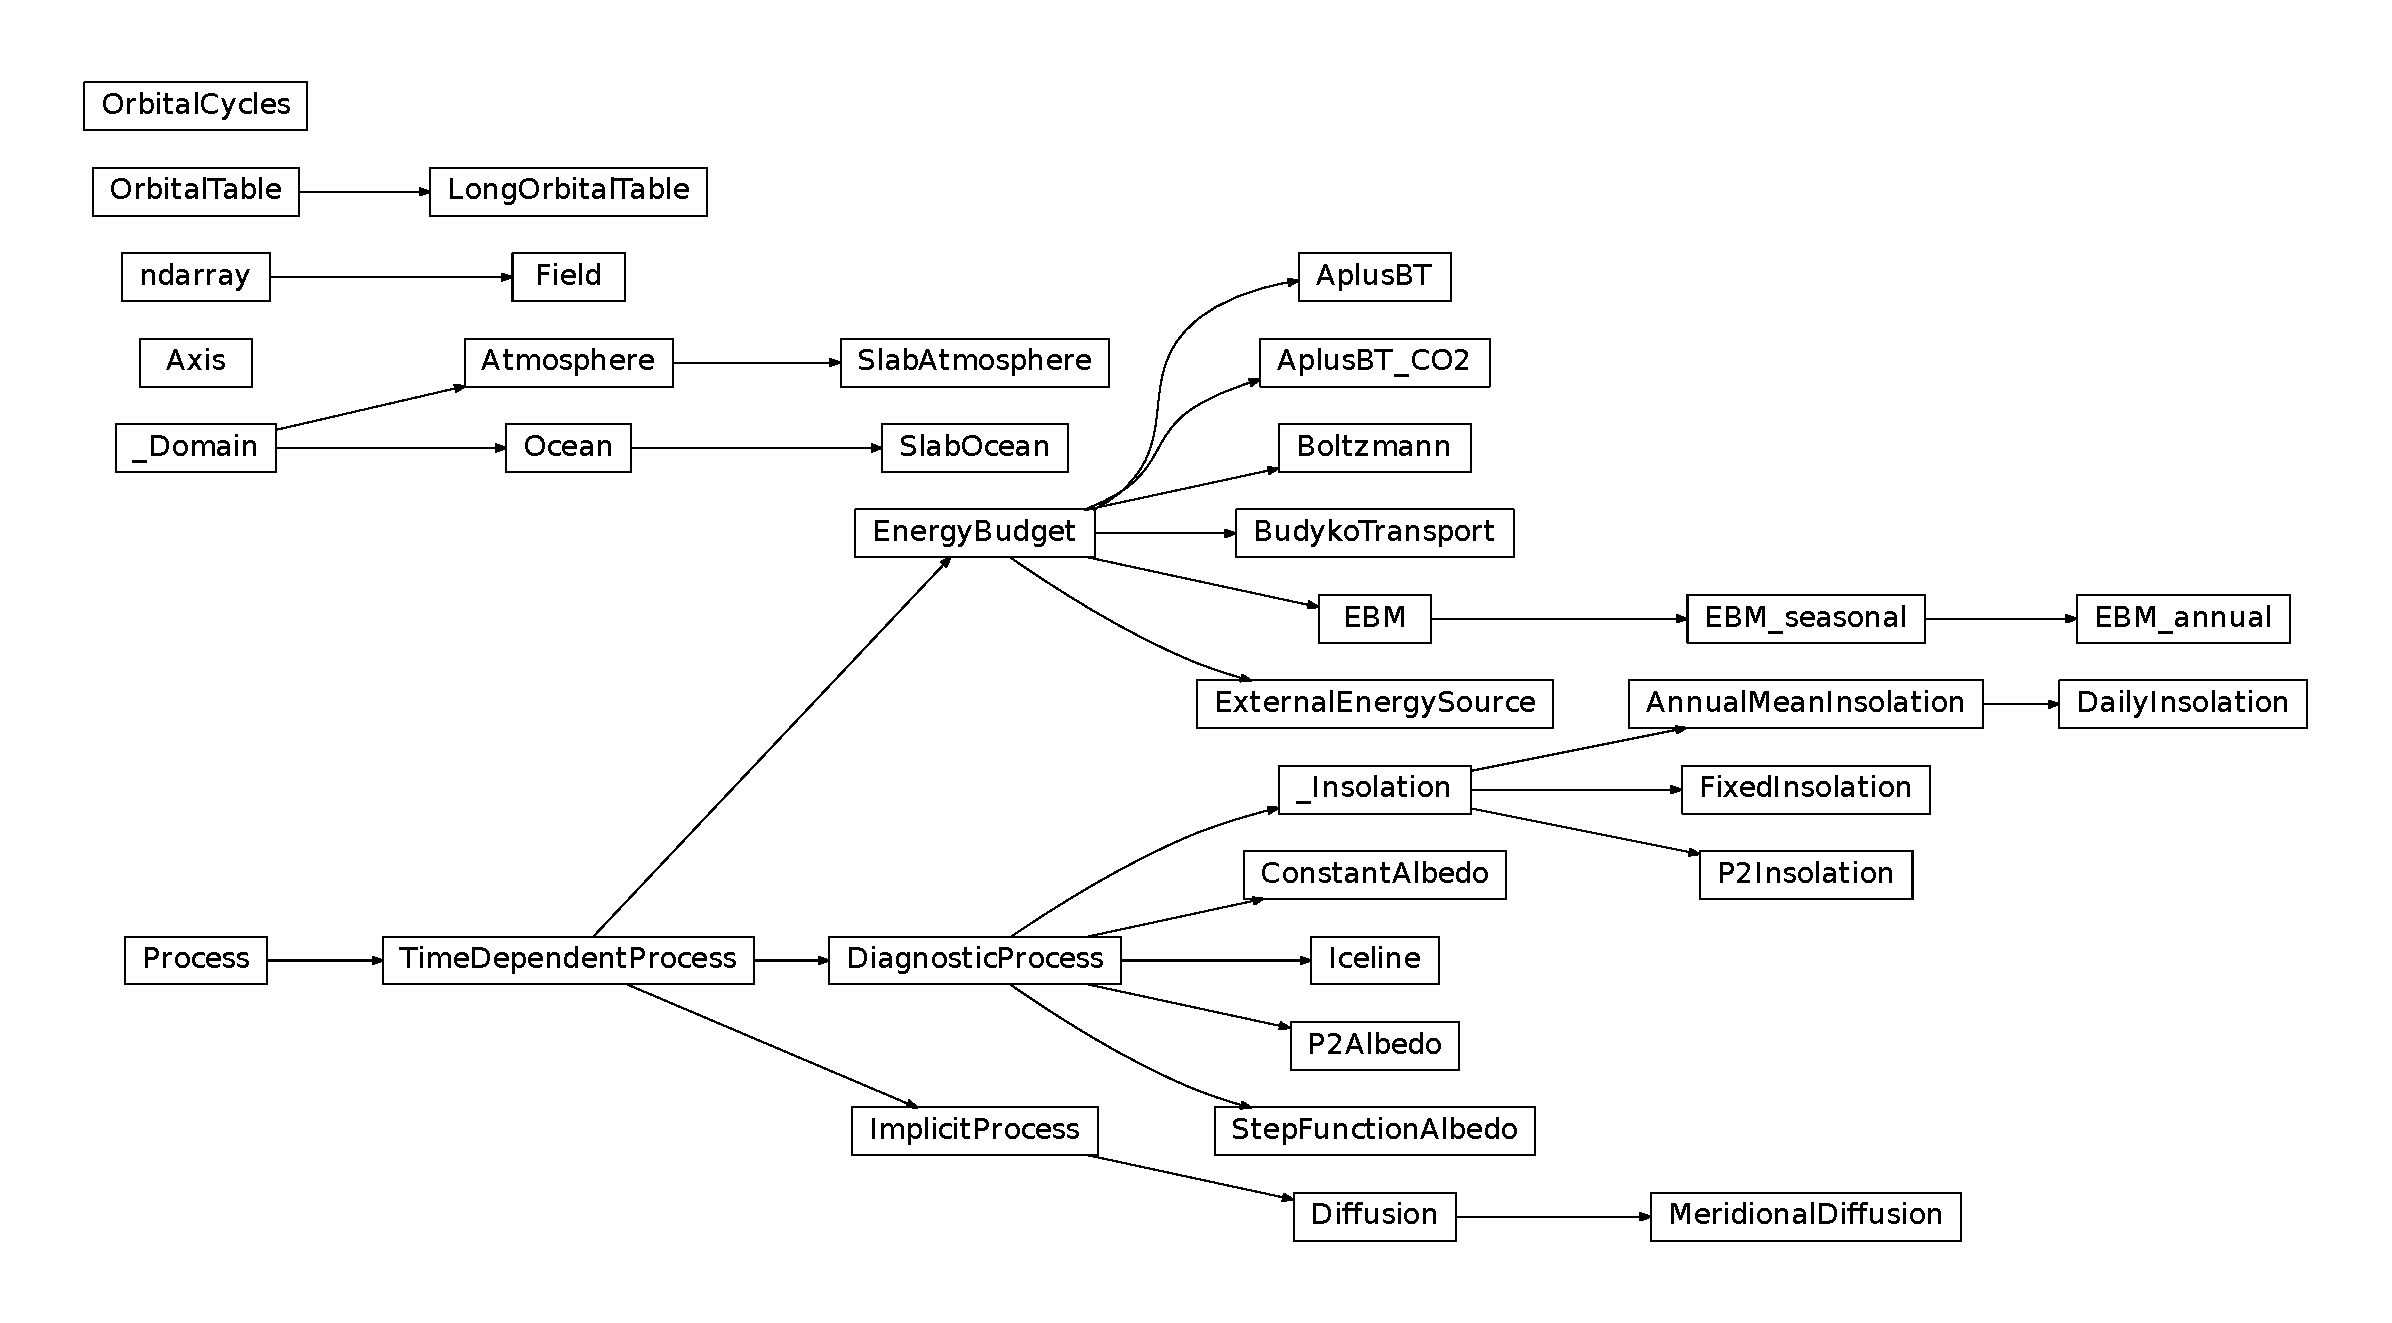
\includegraphics{inheritance-146680b39325a875f0dcfe7f223bdb8225716a47.pdf}


\chapter{References}
\label{references:references}\label{references::doc}\begin{itemize}
\item {} 
A. Berger. Long-term variations of daily insolation and quaternary climatic changes. \emph{Journal of Atmospheric Science}, 35(12):2362–2367, 1978.

\item {} 
A. Berger and M. F. Loutre. Insolation values for the climate of the last 10 million years. \emph{Quaternary Science Reviews}, 10(4):297–317, 1991.

\item {} 
M. I. Budyko. The effect of solar radiation variations on the climate of the earth. \emph{Tellus}, 21(5):611–619, 1969.

\item {} 
Ken Caldeira and James F. Kasting. Susceptibility of the early earth to irreversible glaciation caused by carbon dioxide clouds. \emph{Nature}, 359:226–228, 1992.

\item {} 
J. Laskar, P. Robutel, F. Joutel, M. Gastineau, A. C. M. Correia, and B. Levrard. A long-term numerical solution for the insolation quantities of the earth. \emph{Astronomy \& Astrophysics}, 428:261–285, 2004.

\end{itemize}


\chapter{License}
\label{license::doc}\label{license:license}

\section{climlab}
\label{license:climlab}
The climlab Python package is licensed under MIT License:

\begin{Verbatim}[commandchars=\\\{\}]
The MIT License (MIT)

Copyright (c) 2015 Brian E. J. Rose

Permission is hereby granted, free of charge, to any person obtaining a copy
of this software and associated documentation files (the \PYGZdq{}Software\PYGZdq{}), to deal
in the Software without restriction, including without limitation the rights
to use, copy, modify, merge, publish, distribute, sublicense, and/or sell
copies of the Software, and to permit persons to whom the Software is
furnished to do so, subject to the following conditions:

The above copyright notice and this permission notice shall be included in all
copies or substantial portions of the Software.

THE SOFTWARE IS PROVIDED \PYGZdq{}AS IS\PYGZdq{}, WITHOUT WARRANTY OF ANY KIND, EXPRESS OR
IMPLIED, INCLUDING BUT NOT LIMITED TO THE WARRANTIES OF MERCHANTABILITY,
FITNESS FOR A PARTICULAR PURPOSE AND NONINFRINGEMENT. IN NO EVENT SHALL THE
AUTHORS OR COPYRIGHT HOLDERS BE LIABLE FOR ANY CLAIM, DAMAGES OR OTHER
LIABILITY, WHETHER IN AN ACTION OF CONTRACT, TORT OR OTHERWISE, ARISING FROM,
OUT OF OR IN CONNECTION WITH THE SOFTWARE OR THE USE OR OTHER DEALINGS IN THE
SOFTWARE.
\end{Verbatim}


\section{Documentation}
\label{license:documentation}
The climlab Documentation is licensed under MIT License:

\begin{Verbatim}[commandchars=\\\{\}]
The MIT License (MIT)

Copyright (c) 2016 Moritz Kreuzer, Brian E. J. Rose

Permission is hereby granted, free of charge, to any person obtaining a copy
of this software and associated documentation files (the \PYGZdq{}Software\PYGZdq{}), to deal
in the Software without restriction, including without limitation the rights
to use, copy, modify, merge, publish, distribute, sublicense, and/or sell
copies of the Software, and to permit persons to whom the Software is
furnished to do so, subject to the following conditions:

The above copyright notice and this permission notice shall be included in all
copies or substantial portions of the Software.

THE SOFTWARE IS PROVIDED \PYGZdq{}AS IS\PYGZdq{}, WITHOUT WARRANTY OF ANY KIND, EXPRESS OR
IMPLIED, INCLUDING BUT NOT LIMITED TO THE WARRANTIES OF MERCHANTABILITY,
FITNESS FOR A PARTICULAR PURPOSE AND NONINFRINGEMENT. IN NO EVENT SHALL THE
AUTHORS OR COPYRIGHT HOLDERS BE LIABLE FOR ANY CLAIM, DAMAGES OR OTHER
LIABILITY, WHETHER IN AN ACTION OF CONTRACT, TORT OR OTHERWISE, ARISING FROM,
OUT OF OR IN CONNECTION WITH THE SOFTWARE OR THE USE OR OTHER DEALINGS IN THE
SOFTWARE.
\end{Verbatim}


\chapter{Contact}
\label{contact:contact}\label{contact::doc}

\section{climlab package}
\label{contact:climlab-package}
The climlab package has been developed by Brian Rose:
\begin{quote}

\begin{DUlineblock}{0em}
\item[] \textbf{Brian E. J. Rose}
\item[] Department of Atmospheric and Environmental Sciences
\item[] University at Albany
\item[] \href{mailto:brose@albany.edu}{brose@albany.edu}
\end{DUlineblock}
\end{quote}

Bug reports can be reported through the \href{https://github.com/brian-rose/climlab/issues}{issue tracker} on github.


\section{climlab documentation}
\label{contact:climlab-documentation}
The documentation has been built by Moritz Kreuzer using \href{http://www.sphinx-doc.org}{Sphinx}.
Based on some commentary strings in the source code and a couple of Jupyter Notebooks, this documentation has been developed.

Currently, it covers only the Energy Balance Model relevant parts of the package.
\begin{quote}

\begin{DUlineblock}{0em}
\item[] \textbf{Moritz Kreuzer}
\item[] Potsdam Institut for Climate Impact Research (PIK)
\item[] Potsdam, Germany
\item[] \href{mailto:kreuzer@pik-potsdam.de}{kreuzer@pik-potsdam.de}
\end{DUlineblock}
\end{quote}



\renewcommand{\indexname}{Index}

\end{document}
